\documentclass[11pt]{article}
\usepackage[margin=1in]{geometry}
\usepackage{booktabs}
\usepackage{tabularx}
\usepackage{array}
\usepackage{graphicx}
\usepackage{longtable}
\usepackage{hyperref}
\usepackage{xcolor}
\usepackage{setspace}
\setstretch{1.1}
\newcolumntype{Y}{>{\raggedright\arraybackslash}X}
\newcommand{\taxon}[1]{\emph{#1}}
\newcommand{\dcstsep}{/\allowbreak}
\newcommand{\agpantibioticstatus}{\texttt{Antibiotic\_\allowbreak Status}}
\title{Supplementary Materials\\Inflammatory Bowel Disease-Associated Dominance States in the Human Gut Microbiome}
\author{Pawel Gajer and Jacques Ravel}
\date{}
\newif\ifshowbuildstamp
\showbuildstampfalse
\providecommand{\manuscriptversion}{unversioned}
\providecommand{\manuscriptbuildnumber}{NA}
\providecommand{\manuscriptcommit}{unknown}
\providecommand{\manuscriptbuilddatetime}{unknown}
\InputIfFileExists{../build/manuscript_build_info.tex}{}{}

\begin{document}
\maketitle
\ifshowbuildstamp
\begin{center}
\footnotesize
Built \manuscriptbuilddatetime
\end{center}
\vspace{0.35em}
\fi

\section*{Supplementary Methods}

Outcome flags in the AGP discovery cohort were derived directly from the
\texttt{Phenotype} metadata field by fixed substring matching. The five
outcome variables analyzed in the main manuscript were IBS (\texttt{irritable bowel
syndrome}), IBD (\texttt{inflammatory bowel disease}), autoimmune disease
(\texttt{autoimmune}), acid reflux (\texttt{acid reflux}), and seasonal
allergies (\texttt{seasonal allergies}). For each outcome, samples
without the corresponding outcome-defining phrase served as controls.
These outcome flags were therefore not mutually exclusive across the
discovery cohort.

dCST construction was applied after the discovery feature-retention
filter described in the main manuscript. The labels should therefore be
read as retained-feature dominance states, not as claims about every raw
feature in the original table. Feature names use the deepest informative
SILVA annotation available for each retained feature, which is why the
tables include a mixture of species, genus, family, order, and unresolved
labels.

The AGP discovery phenotype labels are self-reported and do not provide a
uniform treatment-naive clinical IBD classification. IBD subtype, disease
activity, and detailed medication exposure were not consistently
available for adjusted discovery modeling. The coarser AGP
\agpantibioticstatus{} field was available for most age/sex/BMI
complete-case samples and was used in sensitivity analyses that either
added antibiotic status as a categorical covariate or excluded samples
reporting antibiotic use in the previous week, month, or six months. The
AGP associations are therefore interpreted as phenotype-screening
results and are paired with external validation rather than treated as
clinical estimates on their own.

The adjusted frequentist label-level analyses used logistic regression
with age, sex, and BMI as covariates. The adjusted Bayesian follow-up
used \texttt{arm::bayesglm} with the same covariate structure and the
package's default weakly informative prior. For each label we summarize
the adjusted Bayesian fit by the exponentiated coefficient estimate, an
approximate 95\% credible interval based on the posterior standard
error, and the posterior probability that the label coefficient exceeds
0. Unadjusted Bayesian prevalence contrasts were estimated separately
with a beta-binomial model using a Jeffreys prior,
\(\mathrm{Beta}(0.5,0.5)\). BH-adjusted frequentist results are treated
as the primary screen-level evidence, whereas Bayesian estimates are used
as complementary stabilized summaries for sparse labels.

External validation was evaluated in two complementary modes. In the
rebuilt-cohort mode, each external count matrix was filtered and
analyzed independently with the same absorb workflow used for the AGP
discovery cohort. In the direct AGP-derived label-transfer mode,
external samples were mapped onto the canonical local-QZA SILVA
AGP-derived absorb dCST hierarchy after aligning the external taxa to
the AGP retained-feature dictionary. Transfer used the corrected
nearest-lineage-set rule, under which samples are compared against all
realized AGP lineage sets at each nominal depth and stable terminal
lineages remain valid at later nominal depths. The first mode tests
whether disease-associated dominance structure is reproducible when
rebuilt within a cohort; the second tests portability of the
AGP-defined label dictionary itself. Because some external datasets have
repeated samples per subject, we also repeated leading validation tests
after retaining one detected sample per subject. For direct AGP-derived
label transfer, we additionally summarized root-overlap retention and
nominal depth-specific assignment rates by case/control status so that
label-transfer associations could be interpreted alongside transfer
coverage diagnostics.

Supplementary Tables S11A to S11D summarize the clinician-annotated IBD
validation cohorts, with Supplementary Table S11D reporting the exact
sample and subject counts after label filtering, raw
library-quality control, and AGP-overlap restriction. Supplementary
Tables S14A to S18H then organize the rebuilt-cohort and direct
AGP-derived validation associations by dataset and depth. In those
external tables, the frequentist columns report Fisher odds ratios,
exact p-values, and BH-adjusted q-values from the sample-level \(2 \times 2\)
contingency tables, whereas the Bayesian columns report the
corresponding Jeffreys-prior posterior median odds ratio and 95\%
credible interval from the same case/control counts.
Rendered supplement tables are unfiltered; the same full
machine-readable tables are written to the manuscript asset directory as
TSV files.

\section*{Supplementary Results}

\subsection*{AGP Discovery Cohort Setup and Hierarchy}

\noindent\textbf{Supplementary Table S1.} Case and control sample sizes
for the five AGP outcome indicators analyzed in the main manuscript.
Case definitions were derived by fixed substring matching of the AGP
\texttt{Phenotype} field as described in the Methods.

\begin{center}
\footnotesize
\begin{tabularx}{\textwidth}{@{} l r r r r @{}}
\toprule
Phenotype & Cases & Controls & Complete-case cases & Complete-case controls \\
\midrule
IBS & 4,053 & 20,368 & 3,815 & 18,186 \\
IBD & 1,238 & 23,183 & 1,177 & 20,824 \\
Autoimmune disease & 2,734 & 21,687 & 2,586 & 19,415 \\
Acid reflux & 3,444 & 20,977 & 3,237 & 18,764 \\
Seasonal allergies & 9,203 & 15,218 & 8,499 & 13,502 \\
\bottomrule
\end{tabularx}
\end{center}

\noindent\textbf{Supplementary Table S2.} Growth of the canonical
local-QZA SILVA AGP-derived absorb dCST hierarchy and divergence from
the pre-absorption rare-view assignments used during hierarchy
construction.

\begin{center}
\scriptsize
\begin{tabularx}{\textwidth}{@{} r r r r Y r r @{}}
\toprule
Depth & \(n_0\) & Named states & Median size & Largest state (size) & Assignments changed & Changed (\%) \\
\midrule
1 & 50 & 50 & 132.5 & \taxon{Bacteroides~dorei} (8,734) & 1,515 & 6.2 \\
2 & 25 & 158 & 93.5 & \shortstack[l]{\taxon{Bacteroides~dorei}\dcstsep\\\taxon{Faecalibacterium~prausnitzii} (2,320)} & 7,171 & 29.4 \\
3 & 25 & 219 & 92.0 & \shortstack[l]{\taxon{Segatella} sp.\dcstsep\taxon{Bacteroides~dorei}\dcstsep\\\taxon{Faecalibacterium~prausnitzii} (581)} & 14,676 & 60.1 \\
4 & 25 & 221 & 92.0 & \shortstack[l]{\taxon{Faecalibacterium~prausnitzii}\dcstsep\taxon{Agathobacter~faecis}\dcstsep\\\taxon{Bacteroides~dorei} (516)} & 15,687 & 64.2 \\
\bottomrule
\end{tabularx}
\end{center}

\noindent The paper-facing discovery hierarchy stops at depth 4 and uses
\(n_0 = 50, 25, 25, 25\). Because labels follow the deepest informative
retained-feature SILVA annotation, the hierarchy still contains a mix of
species-, genus-, family-, and order-level names, but the canonical
run no longer relies on the older finer-grained \(n_0\) schedule that
continued to depths 5 and 6.

\bigskip

\noindent\textbf{Supplementary Table S3.} Selected AGP self-reported
IBD absorb dominance-lineages highlighting agreement between
frequentist and Bayesian follow-up.

\begin{center}
\footnotesize
\begin{tabularx}{\textwidth}{@{} Y r r Y Y @{}}
\toprule
Label & Depth & \(n\) & Frequentist adjusted OR (95\% CI) & Bayesian adjusted OR (95\% CrI) \\
\midrule
\taxon{[Eubacterium]~eligens~group~eligens} & 1 & 111 & 73.91 (40.51--134.85) & 71.64 (39.60--129.61) \\
\taxon{Alistipes} sp. & 1 & 129 & 5.24 (3.35--8.22) & 5.15 (3.29--8.07) \\
\taxon{Segatella} sp. & 1 & 2,557 & 0.56 (0.45--0.71) & 0.57 (0.45--0.71) \\
\taxon{[Eubacterium]~eligens~group~eligens}\dcstsep\taxon{Bacteroides~dorei} & 2 & 111 & 73.91 (40.51--134.85) & 71.64 (39.60--129.61) \\
\taxon{Bacteroides~dorei}\dcstsep\taxon{[Eubacterium]~eligens~group~eligens} & 3 & 88 & 18.75 (11.82--29.75) & 18.37 (11.61--29.07) \\
\taxon{Alistipes} sp.\dcstsep\taxon{Bacteroides~dorei} & 4 & 129 & 5.24 (3.35--8.22) & 5.15 (3.29--8.07) \\
\bottomrule
\end{tabularx}
\end{center}

\subsection*{Additional AGP Discovery and Sensitivity Analyses}

\noindent\textbf{Acid reflux.} Acid reflux was the clearest additional
non-IBD gastrointestinal branch in the AGP screen. No depth-1 adjusted
label remained q-significant after BH correction, but the signal
sharpened into deeper \taxon{Segatella}- and
\taxon{Bacteroides~dorei}-centered contexts. The strongest adjusted
depth-4 label was
\taxon{Segatella} sp.\dcstsep\taxon{Bacteroides~dorei}\dcstsep\taxon{Faecalibacterium~prausnitzii}\dcstsep\taxon{Agathobacter~faecis}
(adjusted OR 2.21, global \(q = 5.93\times10^{-4}\)), with related
\taxon{Segatella}/\taxon{Bacteroides~dorei}/\taxon{Bacteroides~sartorii}
and \taxon{Bacteroides~dorei}/Rhodospirillales branches also enriched.
Bayesian follow-up retained the same direction across multiple depth-4
descendants after the frequentist screen thinned.
Because reflux symptoms are self-reported and likely influenced by diet,
medication, and upper-gastrointestinal factors, we regard this branch as
hypothesis-generating rather than disease-specific.

\medskip

\noindent\textbf{Seasonal allergies.} Seasonal allergies provided a
complementary immune-linked example outside the core inflammatory
phenotypes. In the canonical AGP rerun, the dominant pattern was
depletion of \taxon{Segatella} sp. and
\taxon{[Eubacterium]~eligens~group~eligens} together with enrichment of
\taxon{Bacteroides~dorei} and \taxon{Bacteroides} sp. At depth 1,
\taxon{Segatella} sp. was depleted (adjusted OR 0.74, global
\(q = 1.46\times10^{-7}\)) and
\taxon{[Eubacterium]~eligens~group~eligens} was likewise depleted,
whereas \taxon{Bacteroides~dorei} and \taxon{Bacteroides} sp. were
enriched. Bayesian follow-up preserved this paired pattern at greater
depth, but we interpret the branch as exploratory rather than as a
fully validated disease axis.

\medskip

\noindent\textbf{Supplementary Table S4.} Representative depth-2
expansions of common AGP-derived depth-1 parents. Shares are percentages
within the selected depth-1 parent and are shown here to give biological
context for the main-text transfer results, especially the
\taxon{Bacteroides~dorei}- and \taxon{Segatella}-linked states
discussed for the canonical AGP IBD follow-up and Halfvarson direct
transfer.

\begin{center}
\scriptsize
\begin{tabularx}{\textwidth}{@{} l Y Y @{}}
\toprule
Depth-1 parent & Representative depth-2 children in AGP & Why this parent is shown \\
\midrule
\taxon{Bacteroides~dorei} &
\taxon{Faecalibacterium~prausnitzii} (2,320; 26.6\%); \taxon{Bacteroides~ovatus} (957; 11.0\%); \taxon{Bacteroides} sp. (711; 8.1\%); \taxon{Agathobacter~faecis} (465; 5.3\%). &
This dominant AGP parent is ecologically heterogeneous. Its common children show that the \taxon{Bacteroides~dorei} state carried into Halfvarson transfer is not one uniform branch, but a family of related commensal contexts. \\
\taxon{Faecalibacterium~prausnitzii} &
\taxon{Bacteroides~dorei} (1,445; 39.0\%); \taxon{Agathobacter~faecis} (645; 17.4\%); \taxon{Segatella} sp. (165; 4.5\%); Christensenellaceae R-7 group sp. (157; 4.2\%). &
This parent most often resolves toward other anaerobe-rich contexts, which helps interpret repeated depletion of \taxon{Faecalibacterium}-centered states as loss of a broader commensal ecological setting rather than only one taxon. \\
\taxon{Segatella} sp. &
\taxon{Faecalibacterium~prausnitzii} (904; 35.4\%); \taxon{Bacteroides~dorei} (690; 27.0\%); Prevotellaceae fam. (253; 9.9\%); \taxon{Agathobacter~faecis} (121; 4.7\%). &
This parent is shown because \taxon{Segatella} depletion was the clearest Halfvarson transfer signal. Its children connect that depleted parent to both \taxon{Faecalibacterium}-rich and \taxon{Bacteroides~dorei}-rich backgrounds. \\
\taxon{Akkermansia~muciniphila} &
\taxon{Bacteroides~dorei} (428; 48.9\%); \taxon{Faecalibacterium~prausnitzii} (126; 14.4\%); UCG-002 sp. (84; 9.6\%); Clostridia UCG-014 ord. (75; 8.6\%). &
Included because \taxon{Akkermansia} depth-1 depletion also recurred in Halfvarson direct transfer, but its AGP child structure remains largely \taxon{Bacteroides~dorei}-linked rather than forming a separate enterobacterial branch. \\
\bottomrule
\end{tabularx}
\end{center}

\bigskip

\noindent\textbf{Supplementary Table S5.} Selected absorb-policy dCST
dominance-lineage follow-up summary across the main-text and
supplementary phenotype branches.

\begin{center}
\scriptsize
\begin{tabularx}{\textwidth}{@{} l Y Y Y @{}}
\toprule
Phenotype & Depthwise omnibus pattern & Representative adjusted labels & Interpretation \\
\midrule
IBD & Strongest omnibus signal in the AGP screen (Cramer's V 0.24 at depth 1, rising to 0.31 by depths 3--4). & Enriched \emph{[Eubacterium] eligens group eligens}, \emph{Alistipes} sp., \emph{Blautia} sp., and \emph{Bifidobacterium breve}; depleted \emph{Segatella} sp. and \emph{Faecalibacterium prausnitzii}; deeper \emph{Bacteroides dorei}-linked descendants recur. & Canonical AGP IBD follow-up is multistate rather than a single broad parent-lineage effect and is used mainly to define the transfer vocabulary. \\
IBS & More modest omnibus structure (Cramer's V 0.08 at depth 1 and 0.12 by depths 3--4). & Enriched \emph{Bacteroides cellulosilyticus} and Lachnospiraceae NK4A136 group bacterium; depleted \emph{Fenollaria} sp., with weaker negative follow-up for \emph{Faecalibacterium prausnitzii}. & Exploratory symptom-defined pattern remains weaker than IBD or autoimmune disease. \\
Autoimmune & Intermediate omnibus structure (Cramer's V 0.17 at depth 1 and 0.23 by depths 3--4). & Enriched \emph{[Eubacterium] eligens group eligens}, \emph{Bacteroides dorei}, and \emph{Alistipes} sp.; depleted \emph{Segatella} sp. & Robust non-IBD signal confirms that the hierarchy is not specific to one disease label. \\
Acid reflux & Weaker omnibus structure (Cramer's V 0.06 at depth 1 and 0.12 by depth 4). & No depth-1 adjusted label remained q-significant; deeper \emph{Segatella} sp./\emph{Bacteroides dorei}/\emph{Faecalibacterium prausnitzii}/\emph{Agathobacter faecis} and related \emph{Bacteroides dorei} contexts were enriched. & The reflux pattern is expressed mainly through deeper retained-feature contexts rather than one dominant depth-1 state. \\
Seasonal allergies & Broad exploratory structure across depths (Cramer's V 0.09 at depth 1 and 0.14 by depths 3--4). & Enriched \emph{Bacteroides dorei} and \emph{Bacteroides} sp.; depleted \emph{Segatella} sp. and \emph{[Eubacterium] eligens group eligens}. & The hierarchy captures a recurrent non-IBD phenotype pattern with both enriched and depleted states. \\
\bottomrule
\end{tabularx}
\end{center}

\bigskip

\noindent\textbf{Supplementary Figure S1.} AGP self-reported IBD
follow-up for representative absorb dCST dominance-lineages under the
canonical local-QZA SILVA hierarchy. Labels were selected from the
current AGP IBD follow-up to provide one representative adjusted state
per depth together with additional strong labels, while avoiding exact
duplicates of the same retained lineage across multiple depths.
Frequentist adjusted odds ratios are shown where the primary adjusted
screen was estimable; Bayesian adjusted odds ratios provide stabilized
directional summaries for the same selected labels. The dashed vertical
line marks an odds ratio of 1.

\begin{center}
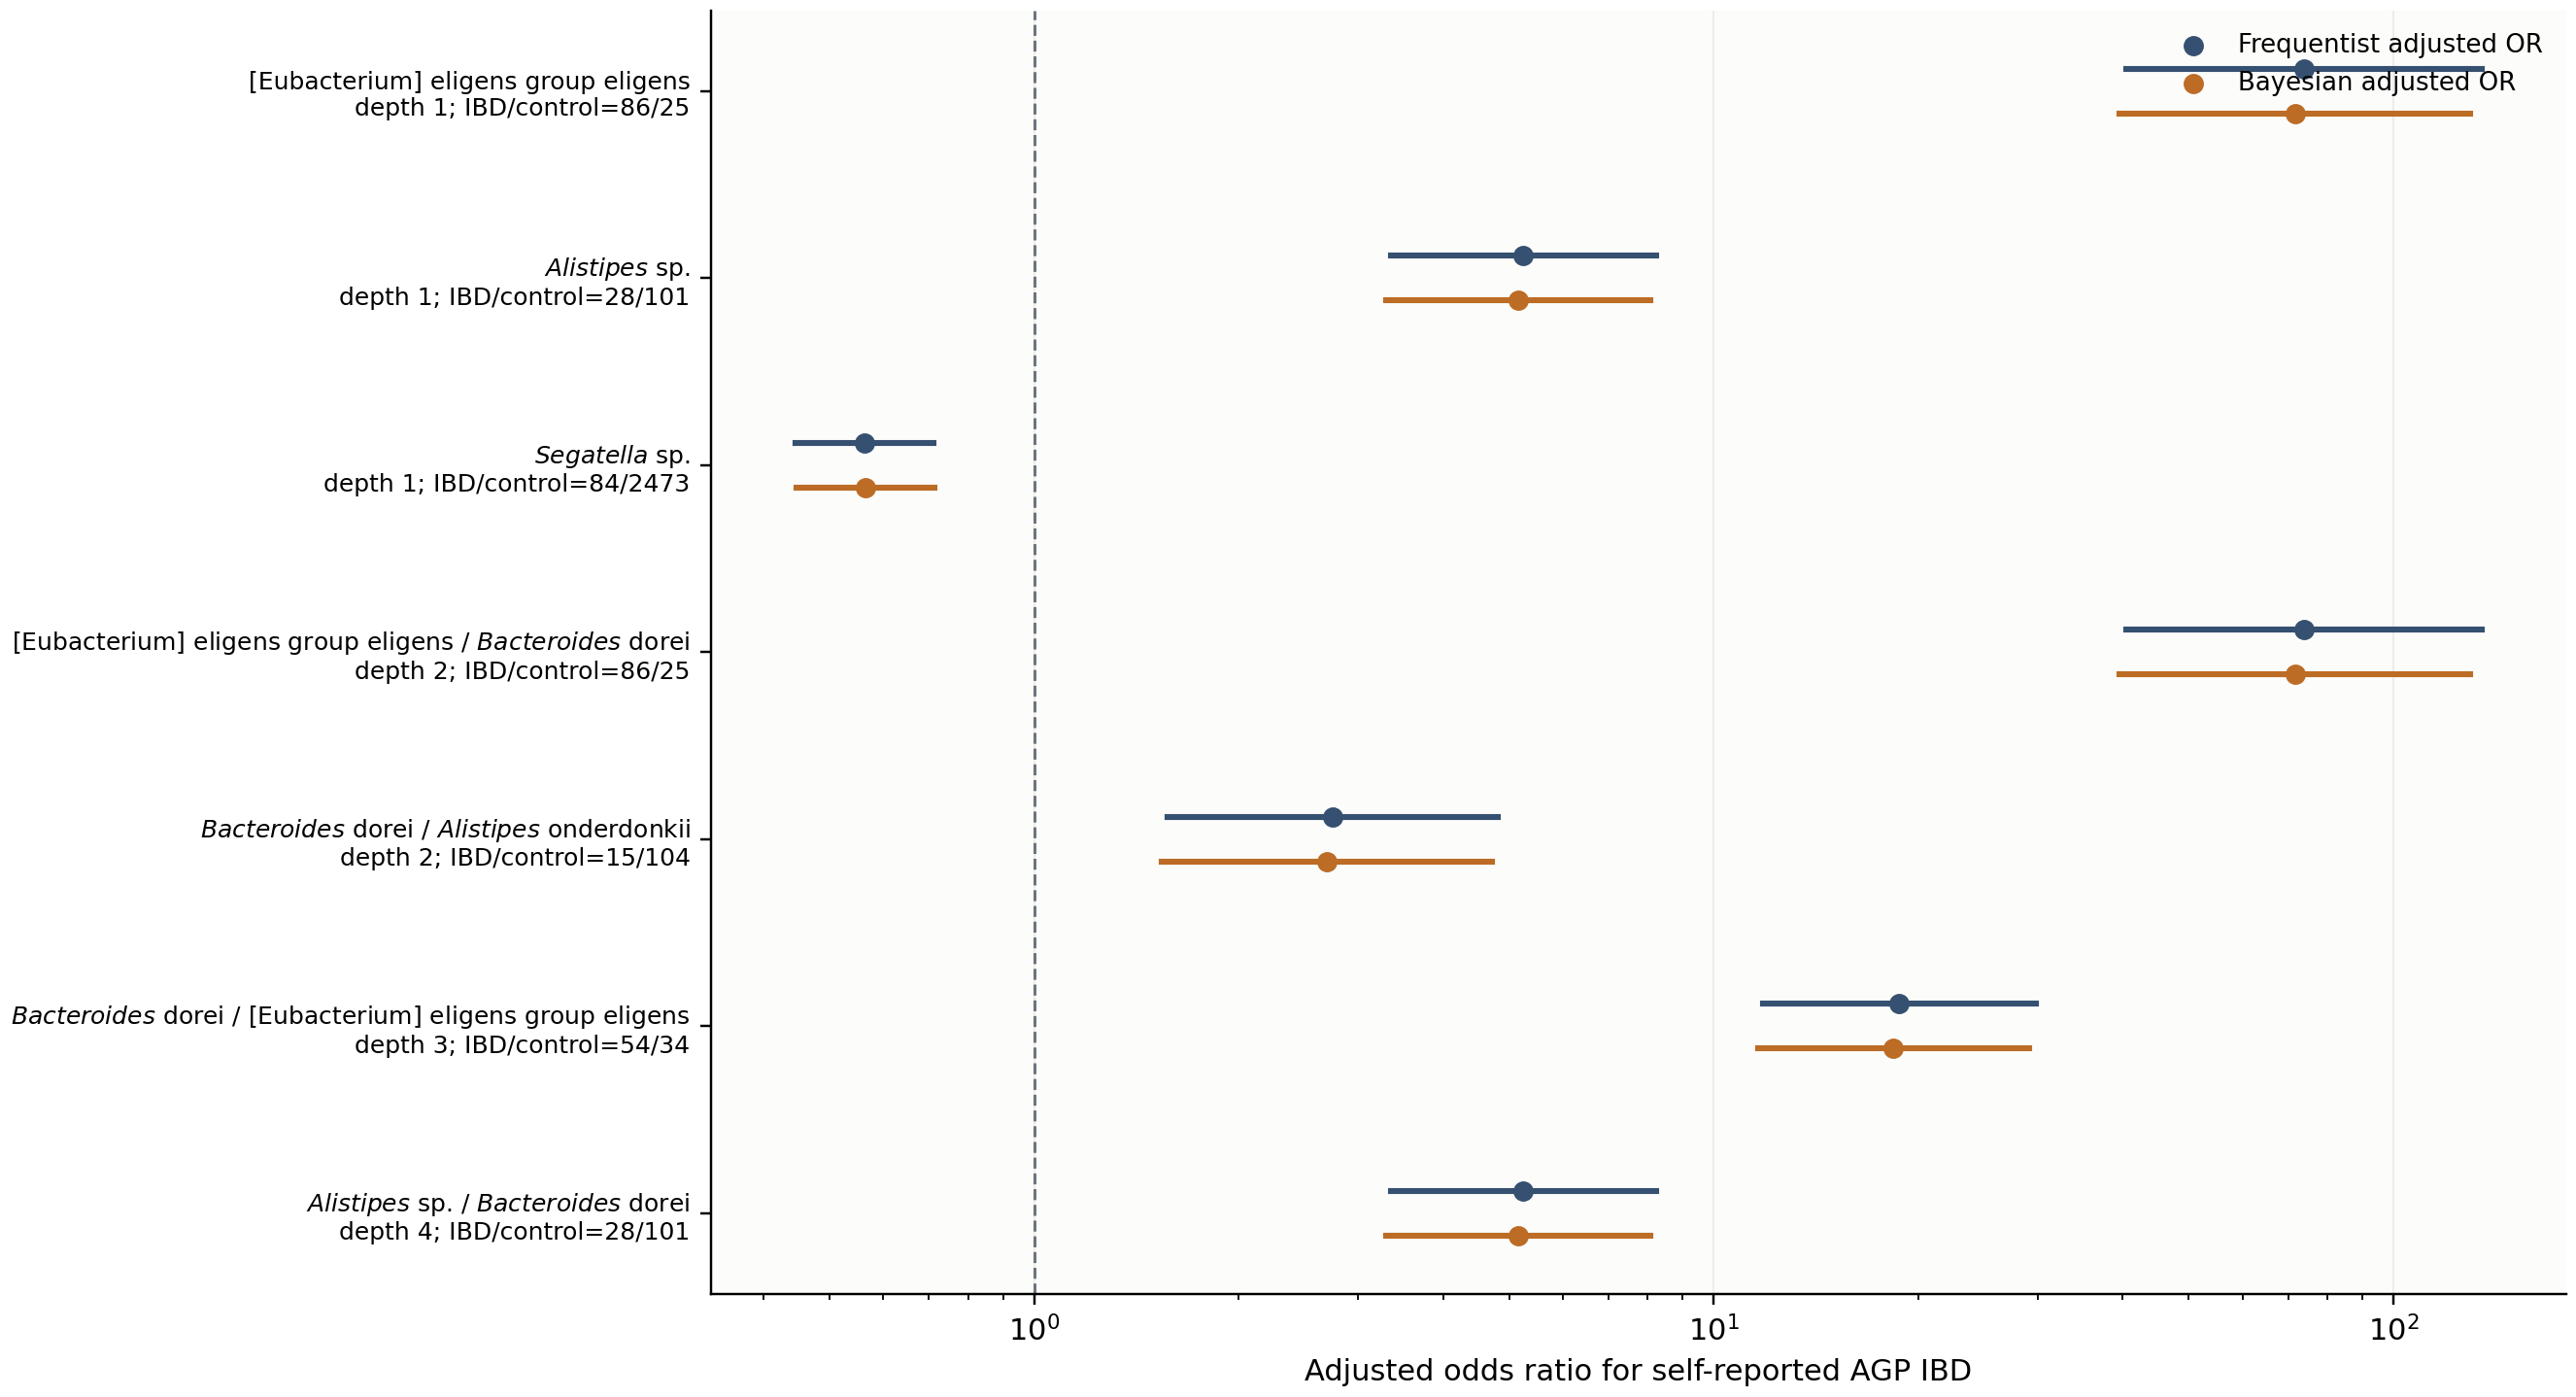
\includegraphics[width=0.92\textwidth]{../assets/figures/FIGURE_S1_agp_ibd_followup_states.png}
\end{center}

\bigskip

\noindent\textbf{Supplementary Table S6.} AGP self-reported IBD
sensitivity analysis after excluding non-IBD controls carrying any other AGP phenotype string
(IBS, autoimmune disease, acid reflux, or seasonal allergies). The
analysis retained all 1,238 IBD cases and 10,572 cleaner controls in
the canonical local-QZA AGP rerun.

\begin{center}
\footnotesize
\begin{tabularx}{\textwidth}{@{} Y r Y Y Y @{}}
\toprule
Label & Depth & Primary analysis & Cleaner-control sensitivity & Interpretation
 \\
\midrule
\emph{[Eubacterium] eligens group eligens} & 1 & 86/25; adjusted OR 73.9, q = 3.3e-44. & 86/15; adjusted OR 82.1, q = 1.3e-20. & Signal retained after cleaner-control restriction. \\
\emph{Alistipes sp.} & 1 & 28/101; adjusted OR 5.24, q = 5.9e-13. & 28/46; adjusted OR 5.21, q = 1.0e-09. & Signal retained after cleaner-control restriction. \\
\emph{Segatella sp.} & 1 & 84/2,473; adjusted OR 0.563, q = 1.5e-06. & 84/1,254; adjusted OR 0.512, q = 4.6e-08. & Signal retained after cleaner-control restriction. \\
\emph{[Eubacterium] eligens group eligens}\dcstsep \emph{Bacteroides dorei} & 2 & 86/25; adjusted OR 73.9, q = 3.3e-44. & 86/15; adjusted OR 82.1, q = 1.3e-20. & Signal retained after cleaner-control restriction. \\
\emph{Bacteroides dorei}\dcstsep \emph{[Eubacterium] eligens group eligens} & 3 & 54/34; adjusted OR 18.8, q = 2.9e-35. & 54/16; adjusted OR 16.7, q = 2.0e-19. & Signal retained after cleaner-control restriction. \\
\emph{Alistipes sp.}\dcstsep \emph{Bacteroides dorei} & 4 & 28/101; adjusted OR 5.24, q = 5.9e-13. & 28/46; adjusted OR 5.21, q = 1.0e-09. & Signal retained after cleaner-control restriction. \\
\bottomrule
\end{tabularx}
\end{center}


\bigskip

\noindent\textbf{Supplementary Table S7.} AGP retained-feature profiles
for selected self-reported IBD dCST dominance-lineages. Values are
median retained-feature relative abundances (\%) for the ordered
components of each selected label. ``Median all'' is the median among
all AGP samples assigned to the label, and ``Median IBD'' is the median
among AGP IBD-case samples assigned to the same label. This table is
intended to make clear that each dCST label is an ordered
retained-feature context rather than a statement that one taxon alone
is globally enriched in disease.

\begin{center}
\scriptsize
\begin{tabularx}{\textwidth}{@{} Y r r Y Y Y @{}}
\toprule
Label & Depth & IBD/control & Ordered retained features & Median all (\%) & Median IBD (\%)
 \\
\midrule
\emph{[Eubacterium] eligens group eligens} & 1 & 86/25 & \emph{[Eubacterium] eligens group eligens} & 100.0 & 100.0 \\
\emph{Alistipes sp.} & 1 & 28/101 & \emph{Alistipes sp.} & 100.0 & 100.0 \\
\emph{Segatella sp.} & 1 & 84/2,473 & \emph{Segatella sp.} & 100.0 & 100.0 \\
\emph{[Eubacterium] eligens group eligens}\dcstsep \emph{Bacteroides dorei} & 2 & 86/25 & \emph{[Eubacterium] eligens group eligens}; \emph{Bacteroides dorei} & 63.4; 36.6 & 59.6; 40.4 \\
\emph{Bacteroides dorei}\dcstsep \emph{[Eubacterium] eligens group eligens} & 3 & 54/34 & \emph{Bacteroides dorei}; \emph{[Eubacterium] eligens group eligens} & 63.9; 36.1 & 57.6; 42.4 \\
\emph{Alistipes sp.}\dcstsep \emph{Bacteroides dorei} & 4 & 28/101 & \emph{Alistipes sp.}; \emph{Bacteroides dorei} & 68.6; 31.4 & 65.2; 34.8 \\
\bottomrule
\end{tabularx}
\end{center}


\newpage

\noindent\textbf{Supplementary Table S8.} AGP antibiotic-status
sensitivity for selected self-reported IBD dCST dominance-lineages. Values are adjusted odds
ratios and selected-label BH-adjusted q-values. The three columns compare
the age/sex/BMI complete-case model, the same model with coarse AGP
antibiotic status added as a categorical covariate, and a
model excluding samples reporting antibiotic use in the previous week,
month, or six months.

\begin{center}
\scriptsize
\begin{tabularx}{\textwidth}{@{} Y r Y Y Y @{}}
\toprule
Label & Depth & Age/sex/BMI & Plus antibiotic status & Excluding recent antibiotics
 \\
\midrule
\emph{[Eubacterium] eligens group eligens} & 1 & OR 73.9; q = 3.3e-44 & OR 76.4; q = 9.4e-45 & OR 123; q = 7.8e-33 \\
\emph{Alistipes sp.} & 1 & OR 5.24; q = 5.9e-13 & OR 5.35; q = 3.6e-13 & OR 5.85; q = 3.1e-13 \\
\emph{Segatella sp.} & 1 & OR 0.563; q = 1.5e-06 & OR 0.558; q = 1.5e-06 & OR 0.488; q = 3.8e-07 \\
\emph{[Eubacterium] eligens group eligens}\dcstsep \emph{Bacteroides dorei} & 2 & OR 73.9; q = 3.3e-44 & OR 76.4; q = 9.4e-45 & OR 123; q = 7.8e-33 \\
\emph{Bacteroides dorei}\dcstsep \emph{[Eubacterium] eligens group eligens} & 3 & OR 18.8; q = 2.9e-35 & OR 19.3; q = 1.3e-35 & OR 22.4; q = 7.4e-34 \\
\emph{Alistipes sp.}\dcstsep \emph{Bacteroides dorei} & 4 & OR 5.24; q = 5.9e-13 & OR 5.35; q = 3.6e-13 & OR 5.85; q = 3.1e-13 \\
\bottomrule
\end{tabularx}
\end{center}


\bigskip

\subsection*{AGP Hierarchy Robustness and Taxonomic Transparency}

\noindent\textbf{Supplementary Table S9.} Absorb-policy robustness for
selected IBD labels. Values compare the absorb dCST view used in the
main manuscript with the pure-policy baseline before low-frequency
dominance patterns are absorbed into retained named states.

\begin{center}
\scriptsize
\begin{tabularx}{\textwidth}{@{} Y r Y Y @{}}
\toprule
Label & Depth & Absorb view & Pure-policy baseline
 \\
\midrule
\emph{[Eubacterium] eligens group eligens} & 1 & OR 69.1; q = 1.0e-88 & OR 74.6; q = 1.9e-85 \\
\emph{Alistipes sp.} & 1 & OR 5.29; q = 6.0e-11 & OR 5.42; q = 1.0e-10 \\
\emph{Segatella sp.} & 1 & OR 0.61; q = 5.6e-06 & OR 0.601; q = 5.4e-06 \\
\emph{[Eubacterium] eligens group eligens}\dcstsep \emph{Bacteroides dorei} & 2 & OR 69.1; q = 1.0e-88 & OR 173; q = 2.2e-42 \\
\emph{Bacteroides dorei}\dcstsep \emph{[Eubacterium] eligens group eligens} & 3 & OR 31; q = 4.0e-47 & OR 34.5; q = 1.9e-47 \\
\emph{Alistipes sp.}\dcstsep \emph{Bacteroides dorei} & 4 & OR 5.29; q = 6.0e-11 & OR 3.24; q = 0.027 \\
\bottomrule
\end{tabularx}
\end{center}


\bigskip

\noindent\textbf{Supplementary Table S10.} Taxonomic-rank transparency
for selected IBD label components. The dCST labels use the deepest
informative retained-feature annotation, so labels can mix taxonomic
ranks.

\begin{center}
\footnotesize
\begin{tabularx}{\textwidth}{@{} l l Y @{}}
\toprule
Component & Rank used by retained feature & SILVA lineage summary
 \\
\midrule
\emph{[Eubacterium] eligens group eligens} & Unresolved & [Eubacterium] eligens group eligens \\
\emph{Alistipes sp.} & Unresolved & Alistipes sp. \\
\emph{Segatella sp.} & Unresolved & Segatella sp. \\
\emph{Bacteroides dorei} & Unresolved & Bacteroides dorei \\
\bottomrule
\end{tabularx}
\end{center}


\subsection*{External IBD Validation Overview}

\noindent\textbf{Supplementary Table S11A.} Rebuilt-cohort external
validation summary. Each external cohort was analyzed independently with
the same absorb-policy dCST workflow used for the discovery cohort.

\begin{center}
\footnotesize
\begin{tabularx}{\textwidth}{@{} l l Y Y @{}}
\toprule
Cohort & Comparison & Best rebuilt signal & Interpretation
 \\
\midrule
Halfvarson 2017 & IBD vs healthy & \emph{Segatella sp.} (depth 1, q = 3.0e-09) & Corrected rebuilt pooled-IBD signal detected. \\
Halfvarson 2017 & Crohn vs healthy & \emph{Segatella sp.} (depth 1, q = 2.6e-05) & Corrected rebuilt Crohn signal detected. \\
Halfvarson 2017 & UC vs healthy & \emph{Bacteroides dorei} (depth 1, q = 3.3e-09) & Corrected rebuilt UC signal detected. \\
HMP2 / IBDMDB & IBD vs healthy & \taxon{Bacteroides}\dcstsep \taxon{Faecalibacterium} (depth 2, q = 0.240) & Directional only in rebuilt mode. \\
Gevers 2014 & Crohn vs healthy & \emph{Faecalibacterium prausnitzii} (depth 1, q = 0.305) & No corrected rebuilt signal. \\
PRJEB84421 & OFG vs healthy & \taxon{Faecalibacterium}\dcstsep \taxon{Bacteroides} (depth 2, q = 0.019) & Corrected rebuilt signal detected. \\
Jacobs 2023 IBS 250bp & IBS vs healthy & \emph{Faecalibacterium prausnitzii}\dcstsep \emph{Bacteroides dorei}\dcstsep \emph{Bacteroides ovatus} (depth 4, q = 0.564) & No corrected rebuilt signal. \\
\bottomrule
\end{tabularx}
\end{center}


\medskip

\noindent\textbf{Supplementary Table S11B.} Direct AGP-derived label-transfer
validation summary. External samples were mapped onto the canonical
local-QZA SILVA AGP-derived absorb dCST hierarchy with the corrected
nearest-lineage-set transfer rule, testing portability of the AGP label
dictionary in the shared taxonomy universe.

\begin{center}
\footnotesize
\begin{tabularx}{\textwidth}{@{} l l Y r Y @{}}
\toprule
Cohort & Comparison & Best AGP-derived label-transfer signal & Depth-2 coverage (\%) & Interpretation
 \\
\midrule
Halfvarson 2017 & IBD vs healthy & \emph{Segatella sp.} (depth 1, q = 1.3e-08) & 99.2 & Corrected AGP-derived pooled-IBD transfer detected. \\
Halfvarson 2017 & Crohn vs healthy & \emph{Segatella sp.} (depth 1, q = 4.1e-07) & 98.4 & Corrected AGP-derived Crohn transfer detected. \\
Halfvarson 2017 & UC vs healthy & \emph{Segatella sp.} (depth 1, q = 5.7e-08) & 100.0 & Corrected AGP-derived UC transfer detected. \\
HMP2 / IBDMDB & IBD vs healthy & \emph{Alistipes sp.} (depth 1, q = 0.742) & 0.0 & Limited mapping constrains transferred signal detection. \\
Gevers 2014 & Crohn vs healthy & \emph{Segatella sp.}\dcstsep \emph{Faecalibacterium prausnitzii}\dcstsep \emph{UCG-002 sp.} (depth 4, q = 0.757) & 86.6 & Samples map into the hierarchy, but no corrected transferred signal. \\
PRJEB84421 & OFG vs healthy & \emph{Blautia sp.} (depth 1, q = 0.002) & 34.7 & Corrected AGP-derived transfer detected. \\
Jacobs 2023 IBS 250bp & IBS vs healthy & \emph{Faecalibacterium prausnitzii}\dcstsep \emph{Akkermansia muciniphila} (depth 2, q = 0.925) & 90.0 & Samples map into the hierarchy, but no corrected transferred signal. \\
\bottomrule
\end{tabularx}
\end{center}


\medskip

\noindent\textbf{Supplementary Table S11C.} External-validation cohort
context for the secondary comparisons summarized in Supplementary Tables
S11A and S11B.

\input{../assets/tables/TABLE_S11C_external_validation_cohort_context.tex}

\medskip

\noindent\textbf{Supplementary Table S11D.} Sample and subject counts for
the clinician-annotated IBD validation cohorts emphasized in the main
text.

\begin{center}
\scriptsize
\begin{tabularx}{\textwidth}{@{} l l r r Y Y Y @{}}
\toprule
Cohort & Comparison & Samples & Subjects & Sample breakdown (CD / UC / healthy) & Subject breakdown (CD / UC / healthy) & Selection strategy
 \\
\midrule
Halfvarson 2017 & IBD vs healthy & 533 & 118 (99 repeated) & CD 200 / UC 279 / healthy 54 & CD 49 / UC 60 / healthy 9 & Primary sample-level analysis; first-sample and bootstrap subject-level sensitivity. \\
Halfvarson 2017 & Crohn vs healthy & 254 & 58 (47 repeated) & CD 200 / UC 0 / healthy 54 & CD 49 / UC 0 / healthy 9 & Primary sample-level analysis; first-sample and bootstrap subject-level sensitivity. \\
Halfvarson 2017 & UC vs healthy & 333 & 69 (61 repeated) & CD 0 / UC 279 / healthy 54 & CD 0 / UC 60 / healthy 9 & Primary sample-level analysis; first-sample and bootstrap subject-level sensitivity. \\
HMP2 / IBDMDB & IBD vs healthy & 166 & 81 (67 repeated) & CD 81 / UC 40 / healthy 45 & CD 37 / UC 22 / healthy 22 & Primary sample-level analysis; first-sample and bootstrap subject-level sensitivity. \\
HMP2 / IBDMDB & Crohn vs healthy & 126 & 59 (51 repeated) & CD 81 / UC 0 / healthy 45 & CD 37 / UC 0 / healthy 22 & Primary sample-level analysis; first-sample and bootstrap subject-level sensitivity. \\
HMP2 / IBDMDB & UC vs healthy & 85 & 44 (37 repeated) & CD 0 / UC 40 / healthy 45 & CD 0 / UC 22 / healthy 22 & Primary sample-level analysis; first-sample and bootstrap subject-level sensitivity. \\
Gevers 2014 & Crohn vs healthy & 396 & 363 (8 repeated) & CD 363 / UC 0 / healthy 33 & CD 331 / UC 0 / healthy 32 & All eligible filtered samples retained; repeated-subject burden is low. \\
\bottomrule
\end{tabularx}
\end{center}


\subsection*{External Validation Diagnostics}

\noindent\textbf{Supplementary Table S12.} Subject-level sensitivity and
bootstrap one-sample-per-subject consensus for external validation.
For each leading comparison, the first two numeric columns show the
sample-level BH-adjusted q-value followed by the corresponding q-value
after retaining the first detected sample per subject. The bootstrap
columns summarize \(B = 1000\) one-sample-per-subject resamples as the
percentage of iterations with \(q < 0.05\), the median adjusted
q-value, and the median Jeffreys-corrected odds ratio with its empirical
95\% percentile interval. In the main-text interpretation, recurrence
\(\geq 50\%\) is treated as the working threshold for subject-level
stability, 25\% to 50\% as suggestive, and \(< 25\%\) as weak with
respect to repeated-sample selection.

\begin{center}
\scriptsize
\begin{tabularx}{\textwidth}{@{} l l Y Y Y Y @{}}
\toprule
Cohort & Comparison & Rebuilt q (sample $\rightarrow$ first subject) & AGP-transfer q (sample $\rightarrow$ first subject) & Rebuilt bootstrap consensus & AGP-transfer bootstrap consensus
 \\
\midrule
Halfvarson 2017 & IBD vs healthy & 3.0e-09 $\rightarrow$ 0.219 & 1.3e-08 $\rightarrow$ 0.652 & 36.8\;(<0.05); med q 0.121; OR 0.171 [0.0753, 0.375] & 9.3\;(<0.05); med q 0.389; OR 0.157 [0.0752, 0.317] \\
Halfvarson 2017 & Crohn vs healthy & 2.6e-05 $\rightarrow$ 0.102 & 4.1e-07 $\rightarrow$ 0.429 & 31.2\;(<0.05); med q 0.102; OR 0.287 [0.122, 0.687] & 9.6\;(<0.05); med q 0.442; OR 0.151 [0.0616, 0.38] \\
Halfvarson 2017 & UC vs healthy & 3.3e-09 $\rightarrow$ 0.075 & 5.7e-08 $\rightarrow$ 0.511 & 58.3\;(<0.05); med q 0.035; OR 5.05 [2.32, 11.5] & 8.5\;(<0.05); med q 0.393; OR 0.171 [0.0652, 0.358] \\
HMP2 / IBDMDB & IBD vs healthy & 0.240 $\rightarrow$ 0.075 & 0.742 $\rightarrow$ 1.000 & 7.7\;(<0.05); med q 0.256; OR 0.433 [0.249, 0.664] & 0.0\;(<0.05); med q 1.000; OR 0.378 [0.12, 0.378] \\
Gevers 2014 & Crohn vs healthy & 0.305 $\rightarrow$ 0.291 & 0.757 $\rightarrow$ 0.787 & 0.0\;(<0.05); med q 0.295; OR 1.75 [1.71, 1.79] & 0.0\;(<0.05); med q 0.821; OR 0.113 [0.109, 0.114] \\
PRJEB84421 & OFG vs healthy & 0.019 $\rightarrow$ 0.019 & 0.002 $\rightarrow$ 0.002 & 100.0\;(<0.05); med q 0.019; OR 0.11 [0.11, 0.11] & 100.0\;(<0.05); med q 0.002; OR 33.5 [33.5, 33.5] \\
\bottomrule
\end{tabularx}
\end{center}


\bigskip

\noindent\textbf{Supplementary Table S13.} Overlap and nominal-assignment
audit for direct AGP-derived label transfer. Coverage is the percentage
of cases or controls assigned a valid AGP lineage set at the specified
nominal depth under the corrected nearest-lineage-set rule.

\begin{center}
\tiny
\begin{tabularx}{\textwidth}{@{} l r r r r Y @{}}
\toprule
Cohort comparison & Depth & Case coverage (\%) & Control coverage (\%) & Fisher p & Note
 \\
\midrule
Halfvarson 2017 IBD vs healthy & 2 & 99.2 & 100.0 & 1.000 & Approx. balanced \\
Halfvarson 2017 IBD vs healthy & 4 & 95.6 & 100.0 & 0.152 & Approx. balanced \\
Halfvarson 2017 UC vs healthy & 2 & 100.0 & 100.0 & 1.000 & Approx. balanced \\
Halfvarson 2017 UC vs healthy & 4 & 97.1 & 100.0 & 0.363 & Approx. balanced \\
HMP2 / IBDMDB IBD vs healthy & 2 & 0.0 & 0.0 & 1.000 & Approx. balanced \\
HMP2 / IBDMDB IBD vs healthy & 4 & 0.0 & 0.0 & 1.000 & Approx. balanced \\
Gevers 2014 Crohn vs healthy & 2 & 85.4 & 100.0 & 0.013 & Controls higher \\
PRJEB84421 OFG vs healthy & 2 & 48.3 & 15.0 & 0.031 & Cases higher \\
Jacobs 2023 IBS 250bp IBS vs healthy & 2 & 91.8 & 89.0 & 0.654 & Approx. balanced \\
\bottomrule
\end{tabularx}
\end{center}


\bigskip

\subsection*{Halfvarson Clinical Stratification Follow-up}

\noindent\textbf{Supplementary Table S13A.} Halfvarson UC extent follow-up. Cases were extensive UC samples (E3) and controls were distal UC samples (E1/E2). The sample-level follow-up included 120 extensive and 173 distal samples from 25 and 35 subjects, respectively. Each row shows the top q-ranked dCST at the specified depth in rebuilt-cohort or direct AGP-derived transfer mode.

\begin{center}
\scriptsize
\begin{tabularx}{\textwidth}{@{} l r r Y Y r r Y @{}}
\toprule
Mode & Depth & Positive/negative samples & Top dCST & Frequentist OR (95\% CI) & \(p\) & \(q\) & Bayesian OR (95\% CrI) \\
\midrule
Rebuilt & 1 & 120/173 & \emph{Bacteroides dorei} & OR 0.554 [0.276, 1.1] & 0.072 & 0.072 & OR 0.553 [0.29, 1.05] \\
Rebuilt & 2 & 120/173 & \emph{Segatella sp.}\dcstsep \emph{Faecalibacterium prausnitzii} & OR 1.81 [0.908, 3.62] & 0.072 & 0.237 & OR 1.81 [0.963, 3.47] \\
Rebuilt & 3 & 120/173 & \emph{Segatella sp.}\dcstsep \emph{Faecalibacterium prausnitzii}\dcstsep \emph{Escherichia-Shigella coli} & OR 0 [0, 0.622] & 0.006 & 0.089 & OR 0.0304 [0.000063, 0.374] \\
Rebuilt & 4 & 120/173 & \emph{Segatella sp.}\dcstsep \emph{Faecalibacterium prausnitzii}\dcstsep \emph{Escherichia-Shigella coli} & OR 0 [0, 0.622] & 0.006 & 0.108 & OR 0.0303 [0.0000718, 0.38] \\
AGP transfer & 1 & 120/173 & \emph{Faecalibacterium prausnitzii} & OR 2.75 [1.26, 6.24] & 0.006 & 0.186 & OR 2.75 [1.33, 5.76] \\
AGP transfer & 2 & 120/173 & \emph{Bacteroides dorei}\dcstsep \emph{Akkermansia muciniphila} & OR inf [1.74, inf] & 0.004 & 0.333 & OR 41.7 [3, 19020] \\
AGP transfer & 3 & 120/173 & \emph{Bacteroides dorei}\dcstsep \emph{Akkermansia muciniphila}\dcstsep \emph{Faecalibacterium prausnitzii} & OR inf [1.74, inf] & 0.004 & 0.442 & OR 40.7 [3.02, 21142] \\
AGP transfer & 4 & 115/170 & \emph{Bacteroides dorei}\dcstsep \emph{Akkermansia muciniphila}\dcstsep \emph{Faecalibacterium prausnitzii} & OR inf [1.79, inf] & 0.004 & 0.407 & OR 41.9 [3, 20321] \\
\bottomrule
\end{tabularx}
\end{center}
\bigskip

\noindent\textbf{Supplementary Table S13B.} Halfvarson Crohn disease location follow-up. Cases were ileal-involved Crohn samples (Montreal L1/L1+L4 and L3/L3+L4) and controls were colonic-only Crohn samples (Montreal L2). The sample-level follow-up included 133 ileal-involved and 77 colonic-only samples from 31 and 18 subjects, respectively. Each row shows the top q-ranked dCST at the specified depth in rebuilt-cohort or direct AGP-derived transfer mode.

\begin{center}
\scriptsize
\begin{tabularx}{\textwidth}{@{} l r r Y Y r r Y @{}}
\toprule
Mode & Depth & Positive/negative samples & Top dCST & Frequentist OR (95\% CI) & \(p\) & \(q\) & Bayesian OR (95\% CrI) \\
\midrule
Rebuilt & 1 & 133/77 & \emph{Bacteroides dorei} & OR 1.59 [0.795, 3.18] & 0.182 & 0.182 & OR 1.6 [0.831, 3.04] \\
Rebuilt & 2 & 133/77 & \emph{Bacteroides dorei}\dcstsep \emph{Faecalibacterium prausnitzii} & OR 0.179 [0.0737, 0.407] & 7.3e-06 & 4.4e-05 & OR 0.178 [0.0805, 0.374] \\
Rebuilt & 3 & 133/77 & \emph{Bacteroides dorei}\dcstsep \emph{Faecalibacterium prausnitzii}\dcstsep \emph{Bacteroides stercoris} & OR 0.179 [0.0737, 0.407] & 7.3e-06 & 6.6e-05 & OR 0.179 [0.0796, 0.378] \\
Rebuilt & 4 & 133/77 & \emph{Bacteroides dorei}\dcstsep \emph{Faecalibacterium prausnitzii}\dcstsep \emph{Bacteroides stercoris}\dcstsep \emph{Agathobacter faecis} & OR 0.194 [0.0518, 0.611] & 0.002 & 0.019 & OR 0.198 [0.0612, 0.551] \\
AGP transfer & 1 & 133/77 & \emph{Faecalibacterium prausnitzii} & OR 0.119 [0.0279, 0.391] & 4.2e-05 & 0.001 & OR 0.121 [0.0355, 0.343] \\
AGP transfer & 2 & 129/77 & \emph{Bacteroides ovatus}\dcstsep \emph{Bacteroides dorei} & OR inf [1.58, inf] & 0.008 & 0.297 & OR 32.5 [2.59, 15243] \\
AGP transfer & 3 & 124/76 & \emph{Bifidobacterium breve}\dcstsep \emph{Bacteroides dorei} & OR 8.72 [1.26, 378] & 0.019 & 0.569 & OR 7.49 [1.61, 87.2] \\
AGP transfer & 4 & 122/75 & \emph{Bifidobacterium breve}\dcstsep \emph{Bacteroides dorei} & OR 8.76 [1.26, 379] & 0.019 & 0.574 & OR 7.73 [1.63, 94.5] \\
\bottomrule
\end{tabularx}
\end{center}
\bigskip

\noindent\textbf{Supplementary Table S13C.} Halfvarson Crohn disease calprotectin follow-up. Cases were Crohn samples with fecal calprotectin $\geq 250$ \textmu g/g and controls were Crohn samples with fecal calprotectin $< 250$ \textmu g/g; this was used as a conservative high-inflammatory-burden split rather than a remission cut-off. The sample-level follow-up included 103 high- and 99 low-calprotectin samples across 49 Crohn subjects; 13 subjects contributed both high- and low-calprotectin samples over time. Each row shows the top q-ranked dCST at the specified depth in rebuilt-cohort or direct AGP-derived transfer mode.

\begin{center}
\scriptsize
\begin{tabularx}{\textwidth}{@{} l r r Y Y r r Y @{}}
\toprule
Mode & Depth & Positive/negative samples & Top dCST & Frequentist OR (95\% CI) & \(p\) & \(q\) & Bayesian OR (95\% CrI) \\
\midrule
Rebuilt & 1 & 103/99 & \emph{Bacteroides dorei} & OR 1.71 [0.853, 3.5] & 0.139 & 0.139 & OR 1.72 [0.896, 3.33] \\
Rebuilt & 2 & 103/99 & \emph{Bacteroides dorei}\dcstsep \emph{Bacteroides uniformis} & OR 2.55 [1.05, 6.7] & 0.029 & 0.176 & OR 2.55 [1.15, 6.15] \\
Rebuilt & 3 & 103/99 & \emph{Segatella sp.}\dcstsep \emph{Faecalibacterium prausnitzii}\dcstsep \emph{Escherichia-Shigella coli} & OR 0.145 [0.0153, 0.677] & 0.005 & 0.044 & OR 0.154 [0.0284, 0.557] \\
Rebuilt & 4 & 103/99 & \emph{Segatella sp.}\dcstsep \emph{Faecalibacterium prausnitzii}\dcstsep \emph{Escherichia-Shigella coli} & OR 0.145 [0.0153, 0.677] & 0.005 & 0.054 & OR 0.153 [0.0257, 0.569] \\
AGP transfer & 1 & 103/99 & \emph{Bacteroides fragilis} & OR 0.242 [0.0419, 0.954] & 0.027 & 0.477 & OR 0.25 [0.0583, 0.791] \\
AGP transfer & 2 & 102/96 & \emph{Segatella sp.}\dcstsep \emph{Bacteroides dorei} & OR 0.0966 [0.00217, 0.721] & 0.008 & 0.456 & OR 0.111 [0.00896, 0.547] \\
AGP transfer & 3 & 100/94 & \emph{Segatella sp.}\dcstsep \emph{Bacteroides dorei}\dcstsep \emph{Faecalibacterium prausnitzii} & OR 0.11 [0.00243, 0.845] & 0.016 & 1.000 & OR 0.126 [0.0107, 0.635] \\
AGP transfer & 4 & 97/94 & \emph{Segatella sp.}\dcstsep \emph{Bacteroides dorei}\dcstsep \emph{Faecalibacterium prausnitzii}\dcstsep \emph{Agathobacter faecis} & OR 0 [0, 0.799] & 0.013 & 0.941 & OR 0.0338 [0.0000714, 0.466] \\
\bottomrule
\end{tabularx}
\end{center}
\bigskip



\noindent\textbf{Supplementary Table S13D.} Subject-aware sensitivity for the Halfvarson clinical stratification follow-up. For UC extent and Crohn location, the case/control definition was fixed at the subject level and the qualifier columns summarize one-sample-per-subject sensitivity for the sample-level top label from Supplementary Tables S13A and S13B. For Crohn calprotectin, the primary analysis remained visit-level; the qualifier columns therefore summarize one-sample-per-subject sensitivity for the same sample-level top label, with high-versus-low status re-evaluated from the selected sample in each resample. The bootstrap column reports the percentage of one-sample-per-subject resamples with $q < 0.05$, together with the median adjusted q-value and the median Jeffreys-corrected odds ratio with its empirical 95\% percentile interval across \(B = 1000\) resamples.

\scriptsize
\setlength{\LTleft}{0pt}
\setlength{\LTright}{0pt}
\begin{longtable}{@{} p{0.12\textwidth} p{0.11\textwidth} p{0.05\textwidth} p{0.25\textwidth} p{0.17\textwidth} p{0.24\textwidth} @{}}
\toprule
Analysis & Mode & Depth & Sample-level top dCST & Sample $\rightarrow$ first-subject \(q\) & Bootstrap one-sample-per-subject consensus \\
\midrule
\endfirsthead
\toprule
Analysis & Mode & Depth & Sample-level top dCST & Sample $\rightarrow$ first-subject \(q\) & Bootstrap one-sample-per-subject consensus \\
\midrule
\endhead
\midrule
\multicolumn{6}{r}{\emph{Continued on next page}} \\
\midrule
\endfoot
\bottomrule
\endlastfoot
UC extent & Rebuilt & 1 & \emph{Bacteroides dorei} & 0.072 $\rightarrow$ 0.728 & 3.2\;(<0.05); med q 0.259; OR 0.429 [0.184, 0.683] \\
UC extent & Rebuilt & 2 & \emph{Segatella sp.}\dcstsep \emph{Faecalibacterium prausnitzii} & 0.237 $\rightarrow$ 1.000 & 0.2\;(<0.05); med q 0.872; OR 2.33 [1.47, 5.43] \\
UC extent & Rebuilt & 3 & \emph{Segatella sp.}\dcstsep \emph{Faecalibacterium prausnitzii}\dcstsep \emph{Escherichia-Shigella coli} & 0.089 $\rightarrow$ 0.817 & 0.0\;(<0.05); med q 1.000; OR 0.451 [0.263, 0.451] \\
UC extent & Rebuilt & 4 & \emph{Segatella sp.}\dcstsep \emph{Faecalibacterium prausnitzii}\dcstsep \emph{Escherichia-Shigella coli} & 0.108 $\rightarrow$ 0.942 & 0.0\;(<0.05); med q 1.000; OR 0.451 [0.263, 0.451] \\
UC extent & AGP transfer & 1 & \emph{Faecalibacterium prausnitzii} & 0.186 $\rightarrow$ 0.926 & 0.0\;(<0.05); med q 0.999; OR 2.45 [0.59, 11] \\
UC extent & AGP transfer & 2 & \emph{Bacteroides dorei}\dcstsep \emph{Akkermansia muciniphila} & 0.333 $\rightarrow$ 1.000 & 0.0\;(<0.05); med q 1.000; OR 4.35 [1.39, 11] \\
UC extent & AGP transfer & 3 & \emph{Bacteroides dorei}\dcstsep \emph{Akkermansia muciniphila}\dcstsep \emph{Faecalibacterium prausnitzii} & 0.442 $\rightarrow$ 1.000 & 0.0\;(<0.05); med q 1.000; OR 4.35 [1.39, 11] \\
UC extent & AGP transfer & 4 & \emph{Bacteroides dorei}\dcstsep \emph{Akkermansia muciniphila}\dcstsep \emph{Faecalibacterium prausnitzii} & 0.407 $\rightarrow$ 1.000 & 0.0\;(<0.05); med q 1.000; OR 4.35 [1.35, 10.7] \\
Crohn location & Rebuilt & 1 & \emph{Bacteroides dorei} & 0.182 $\rightarrow$ 0.708 & 0.0\;(<0.05); med q 0.743; OR 1.01 [0.462, 1.96] \\
Crohn location & Rebuilt & 2 & \emph{Bacteroides dorei}\dcstsep \emph{Faecalibacterium prausnitzii} & 4.4e-05 $\rightarrow$ 0.042 & 49.6\;(<0.05); med q 0.060; OR 0.13 [0.0243, 0.399] \\
Crohn location & Rebuilt & 3 & \emph{Bacteroides dorei}\dcstsep \emph{Faecalibacterium prausnitzii}\dcstsep \emph{Bacteroides stercoris} & 6.6e-05 $\rightarrow$ 0.064 & 33.9\;(<0.05); med q 0.093; OR 0.13 [0.0196, 0.396] \\
Crohn location & Rebuilt & 4 & \emph{Bacteroides dorei}\dcstsep \emph{Faecalibacterium prausnitzii}\dcstsep \emph{Bacteroides stercoris}\dcstsep \emph{Agathobacter faecis} & 0.019 $\rightarrow$ 0.487 & 2.3\;(<0.05); med q 0.491; OR 0.158 [0.0511, 0.574] \\
Crohn location & AGP transfer & 1 & \emph{Faecalibacterium prausnitzii} & 0.001 $\rightarrow$ 1.000 & 0.7\;(<0.05); med q 0.842; OR 0.158 [0.039, 0.593] \\
Crohn location & AGP transfer & 2 & \emph{Bacteroides ovatus}\dcstsep \emph{Bacteroides dorei} & 0.297 $\rightarrow$ 1.000 & 0.0\;(<0.05); med q 1.000; OR 3.14 [0.587, 6.28] \\
Crohn location & AGP transfer & 3 & \emph{Bifidobacterium breve}\dcstsep \emph{Bacteroides dorei} & 0.569 $\rightarrow$ 1.000 & 0.0\;(<0.05); med q 1.000; OR 2.52 [0.636, 7.98] \\
Crohn location & AGP transfer & 4 & \emph{Bifidobacterium breve}\dcstsep \emph{Bacteroides dorei} & 0.574 $\rightarrow$ 1.000 & 0.0\;(<0.05); med q 1.000; OR 2.37 [0.906, 7.55] \\
Crohn calprotectin & Rebuilt & 1 & \emph{Bacteroides dorei} & 0.139 $\rightarrow$ 1.000 & 0.2\;(<0.05); med q 0.725; OR 1.35 [0.558, 2.76] \\
Crohn calprotectin & Rebuilt & 2 & \emph{Bacteroides dorei}\dcstsep \emph{Bacteroides uniformis} & 0.176 $\rightarrow$ 0.616 & 11.4\;(<0.05); med q 0.370; OR 4.1 [1.65, 24.1] \\
Crohn calprotectin & Rebuilt & 3 & \emph{Segatella sp.}\dcstsep \emph{Faecalibacterium prausnitzii}\dcstsep \emph{Escherichia-Shigella coli} & 0.044 $\rightarrow$ 1.000 & 0.0\;(<0.05); med q 0.975; OR 0.488 [0.198, 3] \\
Crohn calprotectin & Rebuilt & 4 & \emph{Segatella sp.}\dcstsep \emph{Faecalibacterium prausnitzii}\dcstsep \emph{Escherichia-Shigella coli} & 0.054 $\rightarrow$ 1.000 & 0.0\;(<0.05); med q 1.000; OR 0.506 [0.198, 2.77] \\
Crohn calprotectin & AGP transfer & 1 & \emph{Bacteroides fragilis} & 0.477 $\rightarrow$ 1.000 & 0.0\;(<0.05); med q 1.000; OR 0.345 [0.0893, 1.13] \\
Crohn calprotectin & AGP transfer & 2 & \emph{Segatella sp.}\dcstsep \emph{Bacteroides dorei} & 0.456 $\rightarrow$ 1.000 & 0.0\;(<0.05); med q 1.000; OR 0.184 [0.104, 0.878] \\
Crohn calprotectin & AGP transfer & 3 & \emph{Segatella sp.}\dcstsep \emph{Bacteroides dorei}\dcstsep \emph{Faecalibacterium prausnitzii} & 1.000 $\rightarrow$ 1.000 & 0.0\;(<0.05); med q 1.000; OR 0.202 [0.13, 0.804] \\
Crohn calprotectin & AGP transfer & 4 & \emph{Segatella sp.}\dcstsep \emph{Bacteroides dorei}\dcstsep \emph{Faecalibacterium prausnitzii}\dcstsep \emph{Agathobacter faecis} & 0.941 $\rightarrow$ 1.000 & 0.0\;(<0.05); med q 1.000; OR 0.291 [0.143, 1.09] \\
\end{longtable}
\normalsize


\subsection*{Gevers Medication Stratification Follow-up}

\noindent\textbf{Supplementary Table S13E.} Exploratory Gevers medication follow-up. The first three analyses asked whether the pediatric Crohn portability boundary persisted after restricting the Gevers stool branch to samples explicitly flagged antibiotic-negative, mesalamine-negative, or steroid-negative. The next three analyses compared medication-positive with medication-negative Crohn-case samples among cases with known status for the same field. Biologics were not evaluable because no analyzed Gevers stool samples were flagged biologics-positive.

\noindent\textbf{Analysis:} Antibiotic-negative Gevers subset. The cohort was restricted to samples explicitly flagged antibiotic-negative, and Crohn disease was compared with healthy controls within that subset. The explicit antibiotic-negative subset contained 321 Crohn samples and 26 healthy-control samples.

\begin{center}
\scriptsize
\begin{tabularx}{\textwidth}{@{} l r r Y Y r r Y @{}}
\toprule
Mode & Depth & Positive/negative samples & Top dCST & Frequentist OR (95\% CI) & \(p\) & \(q\) & Bayesian OR (95\% CrI) \\
\midrule
Rebuilt & 1 & 206/26 & \emph{Faecalibacterium prausnitzii} & OR 2.76 [1.05, 8.1] & 0.036 & 0.107 & OR 2.74 [1.15, 7.19] \\
Rebuilt & 2 & 206/26 & \emph{Faecalibacterium prausnitzii}\dcstsep \emph{Dialister invisus} & OR 3.44 [0.802, 31.1] & 0.121 & 0.392 & OR 3.23 [0.944, 17.5] \\
Rebuilt & 3 & 206/26 & \emph{Blautia obeum}\dcstsep \emph{Bifidobacterium breve} & OR 0.285 [0.0843, 1.12] & 0.037 & 0.456 & OR 0.277 [0.0947, 0.913] \\
Rebuilt & 4 & 206/26 & \emph{Blautia obeum}\dcstsep \emph{Bifidobacterium breve} & OR 0.285 [0.0843, 1.12] & 0.037 & 0.456 & OR 0.28 [0.0967, 0.903] \\
AGP transfer & 1 & 206/26 & \emph{Segatella sp.} & OR 0.272 [0.057, 1.74] & 0.088 & 1.000 & OR 0.26 [0.0693, 1.18] \\
AGP transfer & 2 & 189/26 & \emph{Bacteroides dorei}\dcstsep \emph{Bifidobacterium breve} & OR 0 [0, 5.37] & 0.121 & 1.000 & OR 0.0261 [0.0000511, 0.785] \\
AGP transfer & 3 & 174/24 & \emph{Segatella sp.}\dcstsep \emph{Faecalibacterium prausnitzii}\dcstsep \emph{UCG-002 sp.} & OR 0.13 [0.00902, 1.88] & 0.073 & 1.000 & OR 0.128 [0.0171, 0.967] \\
AGP transfer & 4 & 173/24 & \emph{Segatella sp.}\dcstsep \emph{Faecalibacterium prausnitzii}\dcstsep \emph{UCG-002 sp.} & OR 0.131 [0.00908, 1.89] & 0.073 & 1.000 & OR 0.128 [0.0167, 0.999] \\
\bottomrule
\end{tabularx}
\end{center}
\bigskip

\noindent\textbf{Analysis:} Mesalamine-negative Gevers subset. The cohort was restricted to samples explicitly flagged mesalamine-negative, and Crohn disease was compared with healthy controls within that subset. The explicit mesalamine-negative subset contained 339 Crohn samples and 26 healthy-control samples.

\begin{center}
\scriptsize
\begin{tabularx}{\textwidth}{@{} l r r Y Y r r Y @{}}
\toprule
Mode & Depth & Positive/negative samples & Top dCST & Frequentist OR (95\% CI) & \(p\) & \(q\) & Bayesian OR (95\% CrI) \\
\midrule
Rebuilt & 1 & 224/26 & \emph{Faecalibacterium prausnitzii} & OR 2.75 [1.06, 8.07] & 0.036 & 0.109 & OR 2.73 [1.15, 7.11] \\
Rebuilt & 2 & 224/26 & \emph{Faecalibacterium prausnitzii}\dcstsep \emph{Dialister invisus} & OR 3.8 [0.893, 34.2] & 0.079 & 0.344 & OR 3.57 [1.05, 19.6] \\
Rebuilt & 3 & 224/26 & \emph{Blautia obeum}\dcstsep \emph{Bifidobacterium breve} & OR 0.282 [0.0847, 1.1] & 0.034 & 0.523 & OR 0.273 [0.0969, 0.883] \\
Rebuilt & 4 & 224/26 & \emph{Blautia obeum}\dcstsep \emph{Bifidobacterium breve} & OR 0.282 [0.0847, 1.1] & 0.034 & 0.523 & OR 0.275 [0.0951, 0.888] \\
AGP transfer & 1 & 224/26 & \emph{Segatella sp.} & OR 0.141 [0.0224, 1.02] & 0.026 & 0.715 & OR 0.137 [0.0307, 0.676] \\
AGP transfer & 2 & 198/26 & \emph{Segatella sp.}\dcstsep \emph{Faecalibacterium prausnitzii} & OR 0.187 [0.0204, 2.34] & 0.104 & 1.000 & OR 0.179 [0.0313, 1.24] \\
AGP transfer & 3 & 183/24 & \emph{Segatella sp.}\dcstsep \emph{Faecalibacterium prausnitzii}\dcstsep \emph{UCG-002 sp.} & OR 0.124 [0.00858, 1.79] & 0.067 & 1.000 & OR 0.121 [0.0162, 0.905] \\
AGP transfer & 4 & 182/24 & \emph{Segatella sp.}\dcstsep \emph{Faecalibacterium prausnitzii}\dcstsep \emph{UCG-002 sp.} & OR 0.125 [0.00863, 1.8] & 0.068 & 1.000 & OR 0.123 [0.0163, 0.916] \\
\bottomrule
\end{tabularx}
\end{center}
\bigskip

\noindent\textbf{Analysis:} Steroid-negative Gevers subset. The cohort was restricted to samples explicitly flagged steroid-negative, and Crohn disease was compared with healthy controls within that subset. The explicit steroid-negative subset contained 351 Crohn samples and 26 healthy-control samples.

\begin{center}
\scriptsize
\begin{tabularx}{\textwidth}{@{} l r r Y Y r r Y @{}}
\toprule
Mode & Depth & Positive/negative samples & Top dCST & Frequentist OR (95\% CI) & \(p\) & \(q\) & Bayesian OR (95\% CrI) \\
\midrule
Rebuilt & 1 & 236/26 & \emph{Faecalibacterium prausnitzii} & OR 2.85 [1.09, 8.32] & 0.022 & 0.067 & OR 2.83 [1.19, 7.32] \\
Rebuilt & 2 & 236/26 & \emph{Faecalibacterium prausnitzii}\dcstsep \emph{Dialister invisus} & OR 3.99 [0.941, 35.8] & 0.051 & 0.256 & OR 3.73 [1.1, 20.9] \\
Rebuilt & 3 & 236/26 & \emph{Blautia obeum}\dcstsep \emph{Bifidobacterium breve} & OR 0.287 [0.0874, 1.11] & 0.035 & 0.464 & OR 0.282 [0.0981, 0.915] \\
Rebuilt & 4 & 236/26 & \emph{Blautia obeum}\dcstsep \emph{Bifidobacterium breve} & OR 0.287 [0.0874, 1.11] & 0.035 & 0.464 & OR 0.28 [0.099, 0.897] \\
AGP transfer & 1 & 236/26 & \emph{Segatella sp.} & OR 0.168 [0.0304, 1.15] & 0.035 & 0.976 & OR 0.161 [0.0382, 0.8] \\
AGP transfer & 2 & 207/26 & \emph{Segatella sp.}\dcstsep \emph{Faecalibacterium prausnitzii} & OR 0.179 [0.0194, 2.24] & 0.097 & 1.000 & OR 0.175 [0.031, 1.19] \\
AGP transfer & 3 & 191/24 & \emph{Segatella sp.}\dcstsep \emph{Faecalibacterium prausnitzii}\dcstsep \emph{UCG-002 sp.} & OR 0.119 [0.00822, 1.71] & 0.062 & 1.000 & OR 0.118 [0.0157, 0.881] \\
AGP transfer & 4 & 190/24 & \emph{Segatella sp.}\dcstsep \emph{Faecalibacterium prausnitzii}\dcstsep \emph{UCG-002 sp.} & OR 0.119 [0.00826, 1.72] & 0.063 & 1.000 & OR 0.12 [0.0154, 0.926] \\
\bottomrule
\end{tabularx}
\end{center}
\bigskip

\noindent\textbf{Analysis:} Antibiotic-positive vs antibiotic-negative Crohn samples. Only Crohn-case samples with known antibiotic status were retained, and antibiotic-positive samples were compared with antibiotic-negative samples. Among Crohn-case samples with known antibiotic status, 49 were antibiotic-positive and 206 were antibiotic-negative.

\begin{center}
\scriptsize
\begin{tabularx}{\textwidth}{@{} l r r Y Y r r Y @{}}
\toprule
Mode & Depth & Positive/negative samples & Top dCST & Frequentist OR (95\% CI) & \(p\) & \(q\) & Bayesian OR (95\% CrI) \\
\midrule
Rebuilt & 1 & 49/206 & \emph{Blautia obeum} & OR 1.34 [0.625, 2.77] & 0.468 & 0.871 & OR 1.34 [0.666, 2.6] \\
Rebuilt & 2 & 49/206 & \emph{Blautia obeum} & OR 1.34 [0.625, 2.77] & 0.468 & 0.726 & OR 1.34 [0.675, 2.64] \\
Rebuilt & 3 & 49/206 & \emph{Faecalibacterium prausnitzii}\dcstsep \emph{Bacteroides vulgatus}\dcstsep \emph{Bacteroides fragilis} & OR 0 [0, 1.35] & 0.080 & 0.877 & OR 0.0668 [0.000131, 0.825] \\
Rebuilt & 4 & 49/206 & \emph{Faecalibacterium prausnitzii}\dcstsep \emph{Bacteroides vulgatus}\dcstsep \emph{Bacteroides fragilis} & OR 0 [0, 1.35] & 0.080 & 0.877 & OR 0.0694 [0.00013, 0.844] \\
AGP transfer & 1 & 49/206 & \emph{Enterococcus faecium} & OR 4.26 [1.6, 11.2] & 0.002 & 0.046 & OR 4.29 [1.77, 10] \\
AGP transfer & 2 & 34/189 & \emph{Enterococcus faecium} & OR 6.39 [2.31, 17.6] & 1.3e-04 & 0.005 & OR 6.49 [2.6, 16] \\
AGP transfer & 3 & 32/174 & \emph{Enterococcus faecium} & OR 6.4 [2.28, 17.9] & 1.5e-04 & 0.006 & OR 6.52 [2.6, 16.4] \\
AGP transfer & 4 & 32/173 & \emph{Enterococcus faecium} & OR 6.36 [2.27, 17.7] & 1.6e-04 & 0.006 & OR 6.41 [2.56, 16.2] \\
\bottomrule
\end{tabularx}
\end{center}
\bigskip

\noindent\textbf{Analysis:} Mesalamine-positive vs mesalamine-negative Crohn samples. Only Crohn-case samples with known mesalamine status were retained, and mesalamine-positive samples were compared with mesalamine-negative samples. Among Crohn-case samples with known mesalamine status, 31 were mesalamine-positive and 224 were mesalamine-negative.

\begin{center}
\scriptsize
\begin{tabularx}{\textwidth}{@{} l r r Y Y r r Y @{}}
\toprule
Mode & Depth & Positive/negative samples & Top dCST & Frequentist OR (95\% CI) & \(p\) & \(q\) & Bayesian OR (95\% CrI) \\
\midrule
Rebuilt & 1 & 31/224 & \emph{Blautia obeum} & OR 1.43 [0.564, 3.4] & 0.387 & 0.850 & OR 1.43 [0.618, 3.15] \\
Rebuilt & 2 & 31/224 & \emph{Faecalibacterium prausnitzii}\dcstsep \emph{Segatella sp.} & OR 3.51 [0.74, 13.7] & 0.058 & 0.292 & OR 3.6 [0.993, 11.6] \\
Rebuilt & 3 & 31/224 & \emph{Bacteroides vulgatus}\dcstsep \emph{[Ruminococcus] gnavus group gnavus} & OR 3.51 [0.74, 13.7] & 0.058 & 0.554 & OR 3.62 [0.989, 11.7] \\
Rebuilt & 4 & 31/224 & \emph{Bacteroides vulgatus}\dcstsep \emph{[Ruminococcus] gnavus group gnavus} & OR 3.51 [0.74, 13.7] & 0.058 & 0.554 & OR 3.61 [0.972, 11.8] \\
AGP transfer & 1 & 31/224 & \emph{Gemmiger sp.} & OR 6.41 [1.2, 31.8] & 0.015 & 0.423 & OR 6.5 [1.57, 25.1] \\
AGP transfer & 2 & 25/198 & \emph{Gemmiger sp.} & OR 7.23 [1.33, 36.6] & 0.011 & 0.224 & OR 7.43 [1.8, 29.6] \\
AGP transfer & 3 & 23/183 & \emph{Gemmiger sp.} & OR 7.36 [1.34, 37.6] & 0.010 & 0.232 & OR 7.56 [1.82, 29.8] \\
AGP transfer & 4 & 23/182 & \emph{Gemmiger sp.} & OR 7.32 [1.34, 37.3] & 0.011 & 0.231 & OR 7.42 [1.78, 30.1] \\
\bottomrule
\end{tabularx}
\end{center}
\bigskip

\noindent\textbf{Analysis:} Steroid-positive vs steroid-negative Crohn samples. Only Crohn-case samples with known steroid status were retained, and steroid-positive samples were compared with steroid-negative samples. Among Crohn-case samples with known steroid status, 19 were steroid-positive and 236 were steroid-negative.

\begin{center}
\scriptsize
\begin{tabularx}{\textwidth}{@{} l r r Y Y r r Y @{}}
\toprule
Mode & Depth & Positive/negative samples & Top dCST & Frequentist OR (95\% CI) & \(p\) & \(q\) & Bayesian OR (95\% CrI) \\
\midrule
Rebuilt & 1 & 19/236 & \emph{Faecalibacterium prausnitzii} & OR 0.556 [0.179, 1.59] & 0.244 & 0.419 & OR 0.556 [0.205, 1.41] \\
Rebuilt & 2 & 19/236 & \emph{Faecalibacterium prausnitzii}\dcstsep \emph{Dialister invisus} & OR 0 [0, 0.67] & 0.009 & 0.045 & OR 0.0357 [0.0000705, 0.436] \\
Rebuilt & 3 & 19/236 & \emph{Bacteroides vulgatus}\dcstsep \emph{[Ruminococcus] gnavus group gnavus} & OR 4.2 [0.676, 18.6] & 0.062 & 0.535 & OR 4.37 [0.969, 15.6] \\
Rebuilt & 4 & 19/236 & \emph{Bacteroides vulgatus}\dcstsep \emph{[Ruminococcus] gnavus group gnavus} & OR 4.2 [0.676, 18.6] & 0.062 & 0.535 & OR 4.33 [0.974, 15.7] \\
AGP transfer & 1 & 19/236 & \emph{Gemmiger sp.} & OR 7.07 [1.05, 37] & 0.022 & 0.640 & OR 7.47 [1.55, 30.7] \\
AGP transfer & 2 & 16/207 & \emph{Faecalibacterium prausnitzii}\dcstsep \emph{Bifidobacterium breve} & OR 6.46 [1.29, 27.1] & 0.012 & 0.373 & OR 6.7 [1.7, 23.2] \\
AGP transfer & 3 & 15/191 & \emph{Faecalibacterium prausnitzii}\dcstsep \emph{Bifidobacterium breve} & OR 6.47 [1.28, 27.5] & 0.012 & 0.415 & OR 6.69 [1.7, 24] \\
AGP transfer & 4 & 15/190 & \emph{Faecalibacterium prausnitzii}\dcstsep \emph{Bifidobacterium breve} & OR 6.43 [1.27, 27.4] & 0.012 & 0.411 & OR 6.69 [1.71, 23.9] \\
\bottomrule
\end{tabularx}
\end{center}
\bigskip



\subsection*{Halfvarson Calprotectin Threshold Sensitivity Follow-up}

\noindent\textbf{Supplementary Table S13H.} Thresholded sensitivity for the Halfvarson Crohn calprotectin follow-up. Using the joined Crohn-disease sample universe from the Halfvarson validation matrix, calprotectin was dichotomized at 250~\textmu g/g as a pragmatic high-inflammatory-burden contrast and each label panel was re-evaluated by Fisher's exact test. The table reports the top q-ranked label at each depth and mode.

\begin{center}
\scriptsize
\begin{tabularx}{\textwidth}{@{} l r Y r r Y r r @{}}
\toprule
Mode & Depth & Top dCST & High/low samples & Subjects & OR (95\% CI) & \(p\) & \(q\) \\
\midrule
Rebuilt & 1 & Bacteroides dorei & 103/99 & 49 & 1.715 [0.853, 3.500] & 0.1391 & 0.1391 \\
Rebuilt & 2 & Bacteroides dorei\dcstsep Bacteroides uniformis & 103/99 & 49 & 2.270 [0.956, 5.739] & 0.0513 & 0.2014 \\
Rebuilt & 3 & Segatella sp.\dcstsep Faecalibacterium prausnitzii\dcstsep Escherichia-Shigella coli & 103/99 & 49 & 0.145 [0.015, 0.677] & 0.0049 & 0.0440 \\
Rebuilt & 4 & Segatella sp.\dcstsep Faecalibacterium prausnitzii\dcstsep Escherichia-Shigella coli & 103/99 & 49 & 0.145 [0.015, 0.677] & 0.0049 & 0.0538 \\
AGP transfer & 1 & Bacteroides fragilis & 103/99 & 49 & 0.242 [0.042, 0.954] & 0.0267 & 0.1989 \\
AGP transfer & 2 & Segatella sp.\dcstsep Bacteroides dorei & 102/96 & 49 & 0.097 [0.002, 0.721] & 0.0081 & 0.1058 \\
AGP transfer & 3 & Segatella sp.\dcstsep Bacteroides dorei\dcstsep Faecalibacterium prausnitzii & 100/94 & 49 & 0.110 [0.002, 0.845] & 0.0159 & 0.1844 \\
AGP transfer & 4 & Segatella sp.\dcstsep Bacteroides dorei\dcstsep Faecalibacterium prausnitzii\dcstsep Agathobacter faecis & 97/94 & 48 & 0.000 [0.000, 0.799] & 0.0131 & 0.1438 \\
\bottomrule
\end{tabularx}
\end{center}
\bigskip



\noindent\textbf{Supplementary Table S13I.} Threshold-sweep sensitivity for the Halfvarson Crohn calprotectin follow-up. Using the same Crohn-disease sample universe as Supplementary Table S13H, calprotectin was dichotomized at 100, 150, 200, and 250~\textmu g/g and the top q-ranked label at each depth and mode was recorded. This sweep is intended to show whether the thresholded signal is concentrated only at clearly elevated calprotectin values or remains stable across lower clinical cut-offs.

\scriptsize
\setlength{\LTleft}{0pt}
\setlength{\LTright}{0pt}
\begin{longtable}{@{} r l r p{0.30\textwidth} r r p{0.20\textwidth} r r @{}}
\toprule
Threshold & Mode & Depth & Top dCST & High/low samples & Subjects & OR (95\% CI) & \(p\) & \(q\) \\
\midrule
\endfirsthead
\toprule
Threshold & Mode & Depth & Top dCST & High/low samples & Subjects & OR (95\% CI) & \(p\) & \(q\) \\
\midrule
\endhead
\midrule
\multicolumn{9}{r}{\emph{Continued on next page}} \\
\midrule
\endfoot
\bottomrule
\endlastfoot
100 & Rebuilt & 1 & Segatella sp. & 144/58 & 49 & 0.887 [0.419, 1.936] & 0.7207 & 0.7207 \\
100 & Rebuilt & 2 & Bacteroides dorei\dcstsep Bacteroides ovatus & 144/58 & 49 & 3.832 [1.098, 20.661] & 0.0242 & 0.1455 \\
100 & Rebuilt & 3 & Bacteroides dorei\dcstsep Bacteroides ovatus & 144/58 & 49 & 3.832 [1.098, 20.661] & 0.0242 & 0.2182 \\
100 & Rebuilt & 4 & Bacteroides dorei\dcstsep Bacteroides ovatus & 144/58 & 49 & 3.832 [1.098, 20.661] & 0.0242 & 0.2667 \\
100 & AGP transfer & 1 & Lachnospiraceae fam. & 144/58 & 49 & 0.250 [0.050, 1.100] & 0.0347 & 0.2406 \\
100 & AGP transfer & 2 & Lachnospiraceae fam.\dcstsep Faecalibacterium prausnitzii & 142/56 & 49 & 0.222 [0.033, 1.188] & 0.0422 & 0.2813 \\
100 & AGP transfer & 3 & Lachnospiraceae fam.\dcstsep Faecalibacterium prausnitzii\dcstsep Bacteroides dorei & 139/55 & 49 & 0.223 [0.033, 1.192] & 0.0426 & 0.3315 \\
100 & AGP transfer & 4 & Lachnospiraceae fam.\dcstsep Faecalibacterium prausnitzii\dcstsep Bacteroides dorei & 136/55 & 48 & 0.228 [0.034, 1.219] & 0.0455 & 0.3208 \\
150 & Rebuilt & 1 & Segatella sp. & 132/70 & 49 & 0.790 [0.387, 1.639] & 0.4948 & 0.4948 \\
150 & Rebuilt & 2 & Bacteroides dorei\dcstsep Bacteroides ovatus & 132/70 & 49 & 2.126 [0.782, 6.754] & 0.1366 & 0.7504 \\
150 & Rebuilt & 3 & Segatella sp.\dcstsep Faecalibacterium prausnitzii\dcstsep Escherichia-Shigella coli & 132/70 & 49 & 0.371 [0.101, 1.280] & 0.0829 & 0.6145 \\
150 & Rebuilt & 4 & Segatella sp.\dcstsep Faecalibacterium prausnitzii\dcstsep Escherichia-Shigella coli & 132/70 & 49 & 0.371 [0.101, 1.280] & 0.0829 & 0.7510 \\
150 & AGP transfer & 1 & Lachnospiraceae fam. & 132/70 & 49 & 0.335 [0.067, 1.471] & 0.0980 & 0.4140 \\
150 & AGP transfer & 2 & Bacteroides dorei\dcstsep Bacteroides ovatus & 131/67 & 49 & 3.562 [0.770, 33.483] & 0.0946 & 0.4743 \\
150 & AGP transfer & 3 & Lachnospiraceae fam.\dcstsep Faecalibacterium prausnitzii\dcstsep Bacteroides dorei & 128/66 & 49 & 0.295 [0.044, 1.572] & 0.1238 & 0.5483 \\
150 & AGP transfer & 4 & Lachnospiraceae fam.\dcstsep Faecalibacterium prausnitzii\dcstsep Bacteroides dorei & 125/66 & 48 & 0.302 [0.045, 1.611] & 0.1274 & 0.6760 \\
200 & Rebuilt & 1 & Segatella sp. & 114/88 & 49 & 0.542 [0.267, 1.088] & 0.0698 & 0.0698 \\
200 & Rebuilt & 2 & Segatella sp.\dcstsep Faecalibacterium prausnitzii & 114/88 & 49 & 0.542 [0.267, 1.088] & 0.0698 & 0.3056 \\
200 & Rebuilt & 3 & Segatella sp.\dcstsep Faecalibacterium prausnitzii\dcstsep Escherichia-Shigella coli & 114/88 & 49 & 0.191 [0.033, 0.754] & 0.0098 & 0.0878 \\
200 & Rebuilt & 4 & Segatella sp.\dcstsep Faecalibacterium prausnitzii\dcstsep Escherichia-Shigella coli & 114/88 & 49 & 0.191 [0.033, 0.754] & 0.0098 & 0.1073 \\
200 & AGP transfer & 1 & Lachnospiraceae fam. & 114/88 & 49 & 0.180 [0.018, 0.935] & 0.0222 & 0.1263 \\
200 & AGP transfer & 2 & Segatella sp.\dcstsep Bacteroides dorei & 113/85 & 49 & 0.076 [0.002, 0.569] & 0.0025 & 0.0319 \\
200 & AGP transfer & 3 & Segatella sp.\dcstsep Bacteroides dorei\dcstsep Faecalibacterium prausnitzii & 110/84 & 49 & 0.088 [0.002, 0.679] & 0.0110 & 0.1325 \\
200 & AGP transfer & 4 & Segatella sp.\dcstsep Bacteroides dorei\dcstsep Faecalibacterium prausnitzii\dcstsep Agathobacter faecis & 107/84 & 48 & 0.000 [0.000, 0.643] & 0.0065 & 0.0718 \\
250 & Rebuilt & 1 & Bacteroides dorei & 103/99 & 49 & 1.715 [0.853, 3.500] & 0.1391 & 0.1391 \\
250 & Rebuilt & 2 & Bacteroides dorei\dcstsep Bacteroides uniformis & 103/99 & 49 & 2.270 [0.956, 5.739] & 0.0513 & 0.2014 \\
250 & Rebuilt & 3 & Segatella sp.\dcstsep Faecalibacterium prausnitzii\dcstsep Escherichia-Shigella coli & 103/99 & 49 & 0.145 [0.015, 0.677] & 0.0049 & 0.0440 \\
250 & Rebuilt & 4 & Segatella sp.\dcstsep Faecalibacterium prausnitzii\dcstsep Escherichia-Shigella coli & 103/99 & 49 & 0.145 [0.015, 0.677] & 0.0049 & 0.0538 \\
250 & AGP transfer & 1 & Bacteroides fragilis & 103/99 & 49 & 0.242 [0.042, 0.954] & 0.0267 & 0.1989 \\
250 & AGP transfer & 2 & Segatella sp.\dcstsep Bacteroides dorei & 102/96 & 49 & 0.097 [0.002, 0.721] & 0.0081 & 0.1058 \\
250 & AGP transfer & 3 & Segatella sp.\dcstsep Bacteroides dorei\dcstsep Faecalibacterium prausnitzii & 100/94 & 49 & 0.110 [0.002, 0.845] & 0.0159 & 0.1844 \\
250 & AGP transfer & 4 & Segatella sp.\dcstsep Bacteroides dorei\dcstsep Faecalibacterium prausnitzii\dcstsep Agathobacter faecis & 97/94 & 48 & 0.000 [0.000, 0.799] & 0.0131 & 0.1438 \\
\end{longtable}
\normalsize


\clearpage

\begin{figure}[p]
\centering
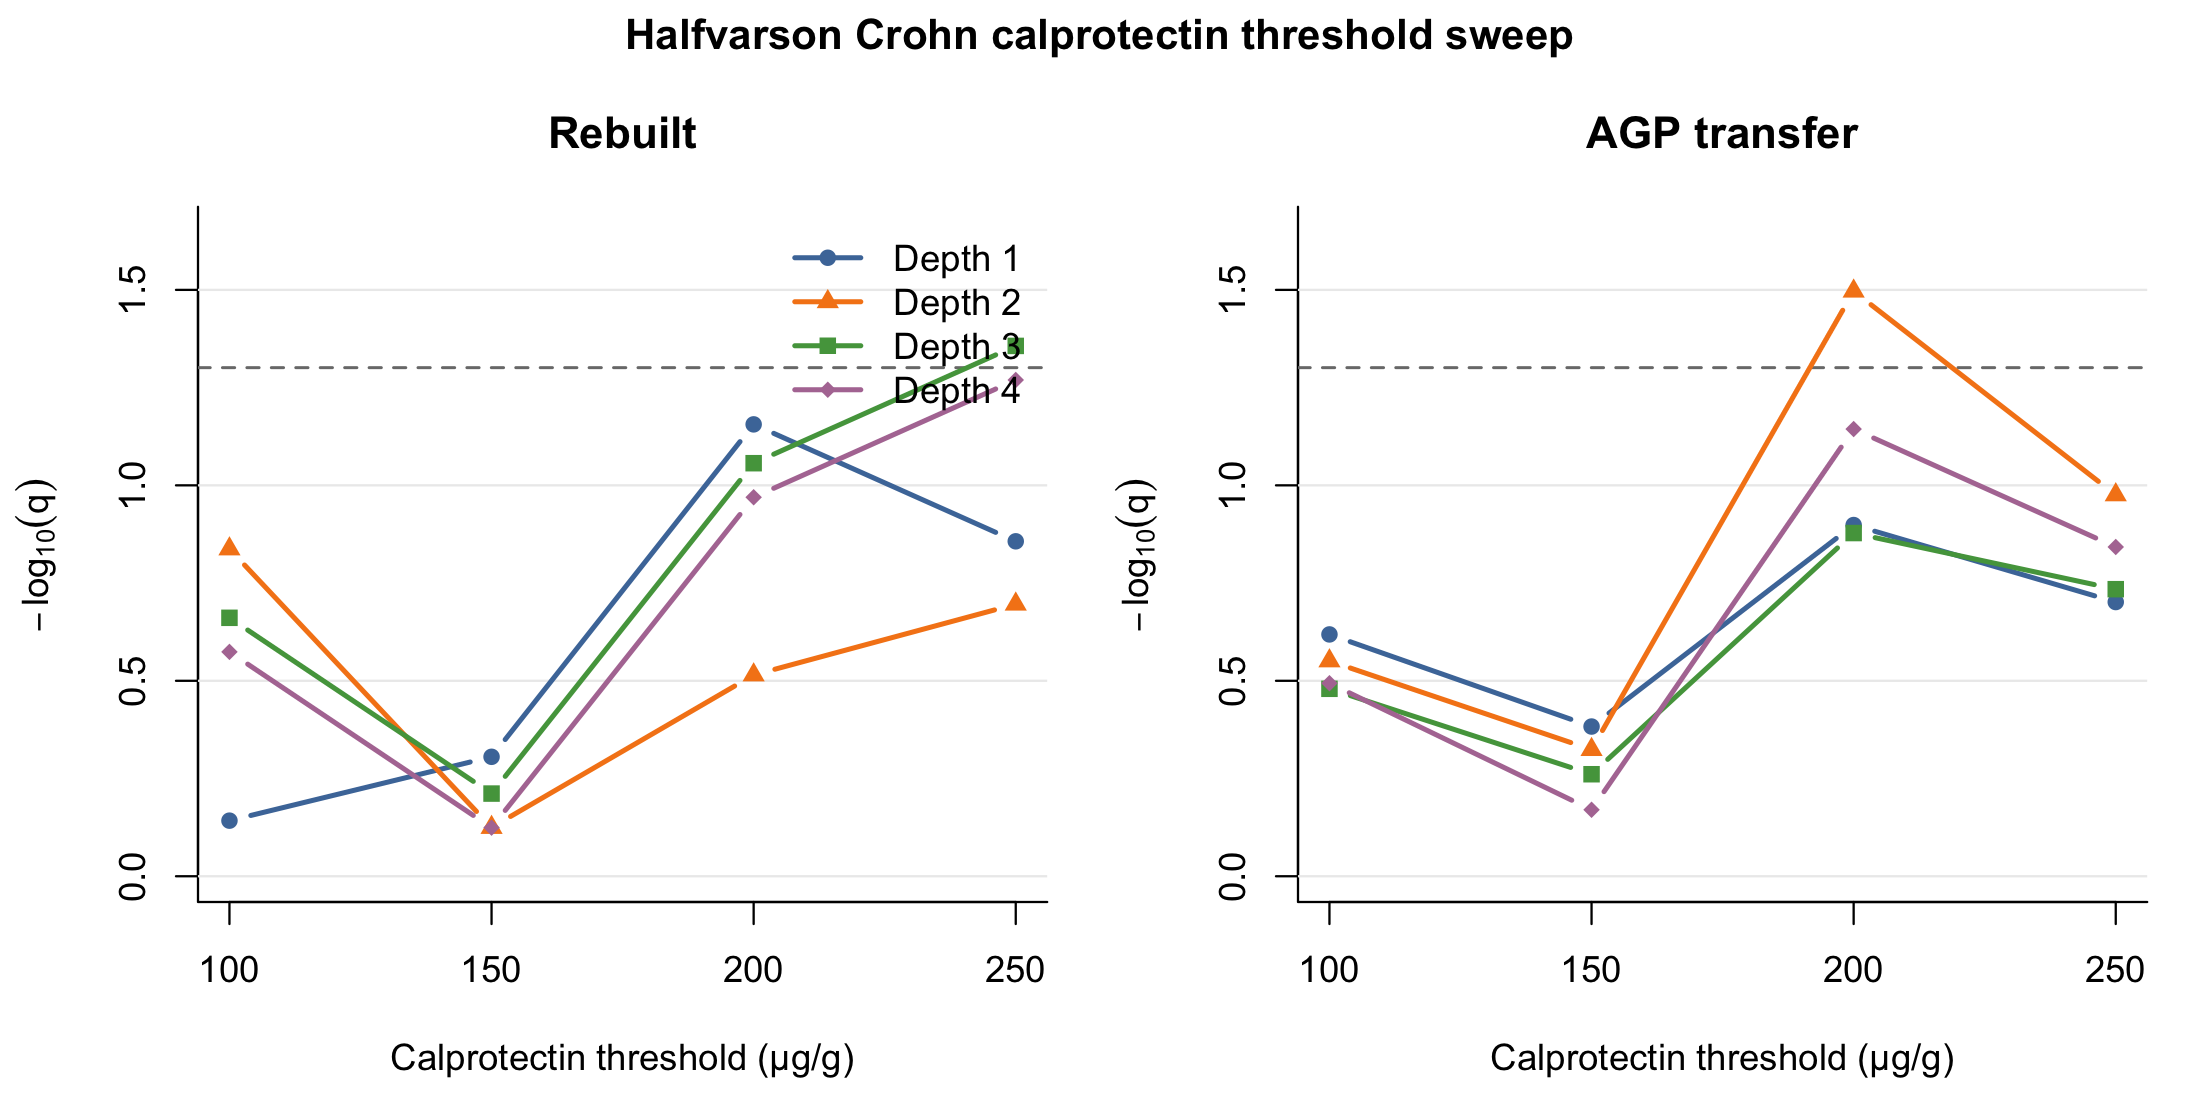
\includegraphics[width=0.94\textwidth]{../assets/figures/FIGURE_S2_halfvarson_calprotectin_threshold_sweep.png}

\medskip

\begin{minipage}{0.94\textwidth}
\small
\noindent\textbf{Supplementary Figure S2.} Threshold-sweep summary for
the Halfvarson Crohn calprotectin follow-up. Each point shows the
BH-adjusted \(q\)-value of the top-ranked label from Supplementary
Table~S13I after dichotomizing calprotectin at 100, 150, 200, or
250~\textmu g/g. The dashed horizontal line marks \(q = 0.05\). This
view is intended to make the threshold pattern readable at a glance:
the rebuilt signal is concentrated more toward the higher-burden end of
the sweep, whereas the AGP-transfer enterobacterial signal recurs at
multiple cut-offs.
\end{minipage}
\end{figure}

\clearpage

\clearpage
\section*{Supplementary Validation Dataset Appendices}

The appendices below organize the external association analyses by validation dataset. Each cohort appendix reports rebuilt-cohort absorb dCST associations followed by direct AGP-derived label-transfer associations across all analyzed depths. Frequentist columns report Fisher odds ratios from the sample-level 2x2 tables, and Bayesian columns report the corresponding Jeffreys-prior posterior median odds ratio and 95\% credible interval derived from the same case/control counts.

\subsection*{Appendix A. Halfvarson 2017}
Longitudinal stool cohort. Primary validation retained all AGP-overlap-filtered samples; one-sample-per-subject sensitivity retained the first available sample per participant.

\noindent\textit{Comparisons analyzed.} IBD vs healthy: 533 samples from 118 subjects (99 subjects with repeated samples); Crohn vs healthy: 254 samples from 58 subjects (47 subjects with repeated samples); UC vs healthy: 333 samples from 69 subjects (61 subjects with repeated samples).

\noindent\textit{Rebuilt-cohort absorb validation tables.}

\noindent\textbf{Supplementary Table S14A.} Rebuilt-cohort absorb dCST associations in Halfvarson 2017 at depth 1. All named absorb dCST labels at this depth are shown. Case/control totals were: IBD vs healthy 479/54; Crohn vs healthy 200/54; UC vs healthy 279/54.

\begingroup
\scriptsize
\setlength{\tabcolsep}{3pt}
\setlength{\LTleft}{0pt}
\setlength{\LTright}{0pt}
\begin{longtable}{@{} p{0.12\textwidth} p{0.26\textwidth} r r p{0.15\textwidth} p{0.07\textwidth} p{0.07\textwidth} p{0.15\textwidth} @{}}
\toprule
Comparison & dCST & Cases & Controls & Frequentist OR (95\% CI) & \(p\) & \(q\) & Bayesian OR (95\% CrI) \\
\midrule
\endfirsthead
\toprule
Comparison & dCST & Cases & Controls & Frequentist OR (95\% CI) & \(p\) & \(q\) & Bayesian OR (95\% CrI) \\
\midrule
\endhead
\bottomrule
\endfoot
IBD vs healthy & Segatella sp. & 70 & 29 & 0.148 (0.0816--0.267) & 6.00e-10 & 3.00e-09 & 0.148 (0.0812--0.266) \\
IBD vs healthy & Bacteroides dorei & 192 & 10 & 2.94 (1.45--5.99) & 0.00173 & 0.00434 & 2.91 (1.49--6.13) \\
IBD vs healthy & Escherichia-Shigella coli & 55 & 0 & NA & 0.00355 & 0.00592 & 31.5 (2.67--1.47e+04) \\
IBD vs healthy & \taxon{Faecalibacterium prausnitzii} & 97 & 9 & 1.27 (0.6--2.69) & 0.595 & 0.743 & 1.26 (0.619--2.78) \\
IBD vs healthy & Bacteroides uniformis & 65 & 6 & 1.26 (0.517--3.05) & 0.832 & 0.832 & 1.22 (0.553--3.3) \\
Crohn vs healthy & Segatella sp. & 49 & 30 & 0.26 (0.139--0.486) & 2.60e-05 & 2.60e-05 & 0.262 (0.139--0.483) \\
Crohn vs healthy & Bacteroides dorei & 151 & 24 & 3.85 (2.06--7.2) & 2.60e-05 & 2.60e-05 & 3.87 (2.1--7.26) \\
UC vs healthy & Bacteroides dorei & 235 & 24 & 6.68 (3.57--12.5) & 3.26e-09 & 3.26e-09 & 6.66 (3.63--12.6) \\
UC vs healthy & Segatella sp. & 44 & 30 & 0.15 (0.0801--0.28) & 3.26e-09 & 3.26e-09 & 0.15 (0.0797--0.277) \\
\end{longtable}
\endgroup
\bigskip

\noindent\textbf{Supplementary Table S14B.} Rebuilt-cohort absorb dCST associations in Halfvarson 2017 at depth 2. All named absorb dCST labels at this depth are shown. Case/control totals were: IBD vs healthy 479/54; Crohn vs healthy 200/54; UC vs healthy 279/54.

\begingroup
\scriptsize
\setlength{\tabcolsep}{3pt}
\setlength{\LTleft}{0pt}
\setlength{\LTright}{0pt}
\begin{longtable}{@{} p{0.12\textwidth} p{0.26\textwidth} r r p{0.15\textwidth} p{0.07\textwidth} p{0.07\textwidth} p{0.15\textwidth} @{}}
\toprule
Comparison & dCST & Cases & Controls & Frequentist OR (95\% CI) & \(p\) & \(q\) & Bayesian OR (95\% CrI) \\
\midrule
\endfirsthead
\toprule
Comparison & dCST & Cases & Controls & Frequentist OR (95\% CI) & \(p\) & \(q\) & Bayesian OR (95\% CrI) \\
\midrule
\endhead
\bottomrule
\endfoot
IBD vs healthy & Segatella sp.\dcstsep \taxon{Faecalibacterium prausnitzii} & 70 & 29 & 0.148 (0.0816--0.267) & 6.00e-10 & 4.20e-09 & 0.148 (0.0818--0.266) \\
IBD vs healthy & Bacteroides dorei\dcstsep Bacteroides ovatus & 58 & 0 & NA & 0.00217 & 0.00758 & 32.7 (2.84--1.57e+04) \\
IBD vs healthy & Escherichia-Shigella coli & 55 & 0 & NA & 0.00355 & 0.00829 & 31.3 (2.71--1.54e+04) \\
IBD vs healthy & Bacteroides dorei\dcstsep \taxon{Faecalibacterium prausnitzii} & 68 & 2 & 4.3 (1.02--18.1) & 0.0316 & 0.0552 & 3.96 (1.25--21.2) \\
IBD vs healthy & \taxon{Faecalibacterium prausnitzii}\dcstsep Bacteroides stercoris & 97 & 9 & 1.27 (0.6--2.69) & 0.595 & 0.832 & 1.25 (0.621--2.75) \\
IBD vs healthy & Bacteroides uniformis & 65 & 6 & 1.26 (0.517--3.05) & 0.832 & 0.836 & 1.22 (0.552--3.22) \\
IBD vs healthy & Bacteroides dorei\dcstsep Bacteroides uniformis & 66 & 8 & 0.919 (0.415--2.03) & 0.836 & 0.836 & 0.91 (0.43--2.13) \\
Crohn vs healthy & Segatella sp.\dcstsep \taxon{Faecalibacterium prausnitzii} & 49 & 30 & 0.26 (0.139--0.486) & 2.60e-05 & 1.56e-04 & 0.26 (0.138--0.486) \\
Crohn vs healthy & Bacteroides dorei\dcstsep Escherichia-Shigella coli & 39 & 0 & NA & 6.30e-05 & 1.89e-04 & 59.5 (4.96--2.78e+04) \\
Crohn vs healthy & Bacteroides dorei\dcstsep Bacteroides ovatus & 28 & 0 & NA & 0.00111 & 0.00223 & 40 (3.33--1.93e+04) \\
Crohn vs healthy & Bacteroides dorei\dcstsep Bifidobacterium breve & 20 & 1 & 5.89 (0.772--44.9) & 0.0547 & 0.0821 & 5.08 (1.11--61.1) \\
Crohn vs healthy & Bacteroides dorei\dcstsep Bacteroides uniformis & 29 & 13 & 0.535 (0.256--1.12) & 0.101 & 0.122 & 0.532 (0.259--1.14) \\
Crohn vs healthy & Bacteroides dorei\dcstsep \taxon{Faecalibacterium prausnitzii} & 35 & 10 & 0.933 (0.429--2.03) & 0.843 & 0.843 & 0.925 (0.438--2.08) \\
UC vs healthy & Segatella sp.\dcstsep \taxon{Faecalibacterium prausnitzii} & 44 & 30 & 0.15 (0.0801--0.28) & 3.26e-09 & 1.96e-08 & 0.15 (0.0796--0.277) \\
UC vs healthy & Bacteroides dorei\dcstsep Agathobacter faecis & 32 & 0 & NA & 0.00432 & 0.0129 & 30.6 (2.53--1.39e+04) \\
UC vs healthy & Bacteroides dorei\dcstsep \taxon{Faecalibacterium prausnitzii} & 92 & 8 & 2.83 (1.28--6.24) & 0.00887 & 0.0177 & 2.8 (1.35--6.51) \\
UC vs healthy & Bacteroides dorei\dcstsep Bacteroides stercoris & 26 & 0 & NA & 0.0119 & 0.0179 & 24.6 (2.05--9.64e+03) \\
UC vs healthy & Bacteroides dorei\dcstsep Akkermansia muciniphila & 11 & 7 & 0.276 (0.102--0.747) & 0.0151 & 0.0181 & 0.272 (0.104--0.766) \\
UC vs healthy & Bacteroides dorei\dcstsep Bacteroides uniformis & 74 & 9 & 1.8 (0.841--3.87) & 0.168 & 0.168 & 1.77 (0.871--3.96) \\
\end{longtable}
\endgroup
\bigskip

\noindent\textbf{Supplementary Table S14C.} Rebuilt-cohort absorb dCST associations in Halfvarson 2017 at depth 3. All named absorb dCST labels at this depth are shown. Case/control totals were: IBD vs healthy 479/54; Crohn vs healthy 200/54; UC vs healthy 279/54.

\begingroup
\scriptsize
\setlength{\tabcolsep}{3pt}
\setlength{\LTleft}{0pt}
\setlength{\LTright}{0pt}
\begin{longtable}{@{} p{0.12\textwidth} p{0.26\textwidth} r r p{0.15\textwidth} p{0.07\textwidth} p{0.07\textwidth} p{0.15\textwidth} @{}}
\toprule
Comparison & dCST & Cases & Controls & Frequentist OR (95\% CI) & \(p\) & \(q\) & Bayesian OR (95\% CrI) \\
\midrule
\endfirsthead
\toprule
Comparison & dCST & Cases & Controls & Frequentist OR (95\% CI) & \(p\) & \(q\) & Bayesian OR (95\% CrI) \\
\midrule
\endhead
\bottomrule
\endfoot
IBD vs healthy & Segatella sp.\dcstsep \taxon{Faecalibacterium prausnitzii}\dcstsep Bifidobacterium breve & 11 & 11 & 0.0919 (0.0376--0.224) & 1.27e-06 & 2.67e-05 & 0.091 (0.0373--0.225) \\
IBD vs healthy & Segatella sp.\dcstsep \taxon{Faecalibacterium prausnitzii}\dcstsep Prevotellaceae fam. & 12 & 8 & 0.148 (0.0575--0.38) & 3.22e-04 & 0.00338 & 0.146 (0.0579--0.384) \\
IBD vs healthy & Bacteroides dorei\dcstsep Bacteroides ovatus\dcstsep Bifidobacterium breve & 58 & 0 & NA & 0.00217 & 0.0152 & 32.9 (2.86--1.33e+04) \\
IBD vs healthy & Bacteroides uniformis\dcstsep Akkermansia muciniphila & 5 & 4 & 0.132 (0.0343--0.507) & 0.0081 & 0.0425 & 0.131 (0.0349--0.526) \\
IBD vs healthy & Segatella sp.\dcstsep \taxon{Faecalibacterium prausnitzii}\dcstsep Bacteroides dorei & 35 & 10 & 0.347 (0.161--0.748) & 0.0162 & 0.0679 & 0.342 (0.166--0.776) \\
IBD vs healthy & Escherichia-Shigella coli\dcstsep Bacteroides ovatus & 31 & 0 & NA & 0.0612 & 0.214 & 16.8 (1.41--7.96e+03) \\
IBD vs healthy & Bacteroides dorei\dcstsep \taxon{Faecalibacterium prausnitzii}\dcstsep Agathobacter faecis & 39 & 1 & 4.7 (0.632--34.9) & 0.108 & 0.323 & 4.02 (0.937--46) \\
IBD vs healthy & \taxon{Faecalibacterium prausnitzii}\dcstsep Bacteroides stercoris\dcstsep UCG-002 sp. & 16 & 4 & 0.432 (0.139--1.34) & 0.134 & 0.329 & 0.418 (0.151--1.43) \\
IBD vs healthy & Bacteroides uniformis\dcstsep Bacteroides dorei & 23 & 0 & NA & 0.153 & 0.329 & 11.9 (1.04--5.51e+03) \\
IBD vs healthy & Escherichia-Shigella coli\dcstsep Bacteroides fragilis & 24 & 0 & NA & 0.157 & 0.329 & 12.8 (1.04--5.37e+03) \\
IBD vs healthy & \taxon{Faecalibacterium prausnitzii}\dcstsep Bacteroides stercoris\dcstsep Agathobacter faecis & 31 & 1 & 3.67 (0.491--27.4) & 0.235 & 0.449 & 3.14 (0.715--36.9) \\
IBD vs healthy & Bacteroides dorei\dcstsep \taxon{Faecalibacterium prausnitzii}\dcstsep Bacteroides uniformis & 29 & 1 & 3.42 (0.456--25.6) & 0.346 & 0.606 & 2.9 (0.667--31.2) \\
IBD vs healthy & Bacteroides uniformis\dcstsep Bacteroides ovatus & 15 & 0 & NA & 0.384 & 0.62 & 7.54 (0.644--3.82e+03) \\
IBD vs healthy & Bacteroides dorei\dcstsep Bacteroides uniformis\dcstsep Bacteroides ovatus & 37 & 6 & 0.67 (0.269--1.67) & 0.425 & 0.637 & 0.656 (0.283--1.73) \\
IBD vs healthy & \taxon{Faecalibacterium prausnitzii}\dcstsep Bacteroides stercoris\dcstsep Bacteroides dorei & 33 & 2 & 1.92 (0.449--8.25) & 0.563 & 0.766 & 1.78 (0.541--9.85) \\
IBD vs healthy & Bacteroides uniformis\dcstsep Bacteroides stercoris & 9 & 0 & NA & 0.608 & 0.766 & 4.58 (0.357--2.22e+03) \\
IBD vs healthy & Segatella sp.\dcstsep \taxon{Faecalibacterium prausnitzii}\dcstsep Escherichia-Shigella coli & 12 & 0 & NA & 0.621 & 0.766 & 6.12 (0.493--2.87e+03) \\
IBD vs healthy & Bacteroides uniformis\dcstsep \taxon{Faecalibacterium prausnitzii} & 13 & 2 & 0.725 (0.159--3.3) & 0.657 & 0.766 & 0.679 (0.183--3.86) \\
IBD vs healthy & Bacteroides dorei\dcstsep Bacteroides uniformis\dcstsep Bacteroides stercoris & 21 & 1 & 2.43 (0.32--18.4) & 0.715 & 0.79 & 2.07 (0.463--24) \\
IBD vs healthy & Bacteroides dorei\dcstsep Bacteroides uniformis\dcstsep Bacteroides eggerthii & 8 & 1 & 0.9 (0.11--7.34) & 1 & 1 & 0.767 (0.156--9.16) \\
IBD vs healthy & \taxon{Faecalibacterium prausnitzii}\dcstsep Bacteroides stercoris\dcstsep Bifidobacterium breve & 17 & 2 & 0.957 (0.215--4.26) & 1 & 1 & 0.874 (0.259--5.01) \\
Crohn vs healthy & Bacteroides dorei\dcstsep Escherichia-Shigella coli & 39 & 0 & NA & 6.30e-05 & 5.67e-04 & 57.7 (5.12--2.33e+04) \\
Crohn vs healthy & Bacteroides dorei\dcstsep Bacteroides ovatus & 28 & 0 & NA & 0.00111 & 0.0046 & 38.5 (3.3--1.76e+04) \\
Crohn vs healthy & Segatella sp.\dcstsep \taxon{Faecalibacterium prausnitzii}\dcstsep Bifidobacterium breve & 13 & 12 & 0.243 (0.104--0.571) & 0.00153 & 0.0046 & 0.243 (0.102--0.578) \\
Crohn vs healthy & Segatella sp.\dcstsep \taxon{Faecalibacterium prausnitzii}\dcstsep Prevotellaceae fam. & 6 & 8 & 0.178 (0.0588--0.538) & 0.00272 & 0.00613 & 0.18 (0.0571--0.537) \\
Crohn vs healthy & Segatella sp.\dcstsep \taxon{Faecalibacterium prausnitzii}\dcstsep Bacteroides dorei & 15 & 10 & 0.357 (0.15--0.847) & 0.0356 & 0.064 & 0.353 (0.152--0.87) \\
Crohn vs healthy & Segatella sp.\dcstsep \taxon{Faecalibacterium prausnitzii}\dcstsep Escherichia-Shigella coli & 15 & 0 & NA & 0.046 & 0.069 & 19.3 (1.6--8.86e+03) \\
Crohn vs healthy & Bacteroides dorei\dcstsep Bifidobacterium breve & 20 & 1 & 5.89 (0.772--44.9) & 0.0547 & 0.0704 & 5.01 (1.12--56.8) \\
Crohn vs healthy & Bacteroides dorei\dcstsep Bacteroides uniformis & 29 & 13 & 0.535 (0.256--1.12) & 0.101 & 0.114 & 0.534 (0.256--1.13) \\
Crohn vs healthy & Bacteroides dorei\dcstsep \taxon{Faecalibacterium prausnitzii}\dcstsep Bacteroides stercoris & 35 & 10 & 0.933 (0.429--2.03) & 0.843 & 0.843 & 0.921 (0.438--2.1) \\
UC vs healthy & Segatella sp.\dcstsep \taxon{Faecalibacterium prausnitzii}\dcstsep Bifidobacterium breve & 4 & 12 & 0.0509 (0.0157--0.165) & 1.17e-07 & 1.64e-06 & 0.0524 (0.0148--0.155) \\
UC vs healthy & Segatella sp.\dcstsep \taxon{Faecalibacterium prausnitzii}\dcstsep Prevotellaceae fam. & 8 & 8 & 0.17 (0.0607--0.475) & 0.00132 & 0.00712 & 0.17 (0.0602--0.475) \\
UC vs healthy & Bacteroides dorei\dcstsep Bacteroides uniformis\dcstsep Bacteroides ovatus & 37 & 0 & NA & 0.00153 & 0.00712 & 35.7 (3.18--1.69e+04) \\
UC vs healthy & Bacteroides dorei\dcstsep Agathobacter faecis & 32 & 0 & NA & 0.00432 & 0.0151 & 31.4 (2.62--1.68e+04) \\
UC vs healthy & Bacteroides dorei\dcstsep \taxon{Faecalibacterium prausnitzii}\dcstsep Bacteroides uniformis & 70 & 5 & 3.28 (1.26--8.57) & 0.0118 & 0.0278 & 3.19 (1.35--9.35) \\
UC vs healthy & Bacteroides dorei\dcstsep Bacteroides stercoris\dcstsep Bacteroides uniformis & 26 & 0 & NA & 0.0119 & 0.0278 & 24.6 (2.08--1.03e+04) \\
UC vs healthy & Bacteroides dorei\dcstsep Akkermansia muciniphila & 11 & 7 & 0.276 (0.102--0.747) & 0.0151 & 0.0302 & 0.274 (0.104--0.78) \\
UC vs healthy & Segatella sp.\dcstsep \taxon{Faecalibacterium prausnitzii}\dcstsep Bacteroides dorei & 22 & 10 & 0.377 (0.167--0.849) & 0.0225 & 0.0394 & 0.374 (0.171--0.862) \\
UC vs healthy & Bacteroides dorei\dcstsep Bacteroides uniformis\dcstsep \taxon{Faecalibacterium prausnitzii} & 19 & 8 & 0.42 (0.174--1.02) & 0.0582 & 0.0905 & 0.416 (0.178--1.05) \\
UC vs healthy & Bacteroides dorei\dcstsep Bacteroides uniformis\dcstsep Bacteroides eggerthii & 8 & 0 & NA & 0.363 & 0.479 & 7.4 (0.558--3.34e+03) \\
UC vs healthy & Segatella sp.\dcstsep \taxon{Faecalibacterium prausnitzii}\dcstsep Escherichia-Shigella coli & 10 & 0 & NA & 0.376 & 0.479 & 9.11 (0.718--4.55e+03) \\
UC vs healthy & Bacteroides dorei\dcstsep \taxon{Faecalibacterium prausnitzii}\dcstsep Bacteroides thetaiotaomicron & 12 & 1 & 2.38 (0.303--18.7) & 0.701 & 0.818 & 2.04 (0.428--24.4) \\
UC vs healthy & Bacteroides dorei\dcstsep Bacteroides uniformis\dcstsep Bacteroides cellulosilyticus & 10 & 1 & 1.97 (0.247--15.7) & 1 & 1 & 1.7 (0.35--20.2) \\
UC vs healthy & Bacteroides dorei\dcstsep \taxon{Faecalibacterium prausnitzii}\dcstsep Muribaculaceae fam. & 10 & 2 & 0.967 (0.206--4.54) & 1 & 1 & 0.899 (0.24--5.17) \\
\end{longtable}
\endgroup
\bigskip

\noindent\textbf{Supplementary Table S14D.} Rebuilt-cohort absorb dCST associations in Halfvarson 2017 at depth 4. All named absorb dCST labels at this depth are shown. Case/control totals were: IBD vs healthy 479/54; Crohn vs healthy 200/54; UC vs healthy 279/54.

\begingroup
\scriptsize
\setlength{\tabcolsep}{3pt}
\setlength{\LTleft}{0pt}
\setlength{\LTright}{0pt}
\begin{longtable}{@{} p{0.12\textwidth} p{0.26\textwidth} r r p{0.15\textwidth} p{0.07\textwidth} p{0.07\textwidth} p{0.15\textwidth} @{}}
\toprule
Comparison & dCST & Cases & Controls & Frequentist OR (95\% CI) & \(p\) & \(q\) & Bayesian OR (95\% CrI) \\
\midrule
\endfirsthead
\toprule
Comparison & dCST & Cases & Controls & Frequentist OR (95\% CI) & \(p\) & \(q\) & Bayesian OR (95\% CrI) \\
\midrule
\endhead
\bottomrule
\endfoot
IBD vs healthy & Segatella sp.\dcstsep \taxon{Faecalibacterium prausnitzii}\dcstsep Bifidobacterium breve & 11 & 11 & 0.0919 (0.0376--0.224) & 1.27e-06 & 2.67e-05 & 0.092 (0.0371--0.226) \\
IBD vs healthy & Segatella sp.\dcstsep \taxon{Faecalibacterium prausnitzii}\dcstsep Prevotellaceae fam. & 12 & 8 & 0.148 (0.0575--0.38) & 3.22e-04 & 0.00338 & 0.148 (0.0584--0.39) \\
IBD vs healthy & Bacteroides dorei\dcstsep Bacteroides ovatus\dcstsep Bifidobacterium breve & 58 & 0 & NA & 0.00217 & 0.0152 & 33.7 (2.85--1.55e+04) \\
IBD vs healthy & Bacteroides uniformis\dcstsep Akkermansia muciniphila & 5 & 4 & 0.132 (0.0343--0.507) & 0.0081 & 0.0425 & 0.131 (0.035--0.512) \\
IBD vs healthy & Segatella sp.\dcstsep \taxon{Faecalibacterium prausnitzii}\dcstsep Bacteroides dorei & 35 & 10 & 0.347 (0.161--0.748) & 0.0162 & 0.0679 & 0.343 (0.165--0.757) \\
IBD vs healthy & Escherichia-Shigella coli\dcstsep Bacteroides ovatus & 31 & 0 & NA & 0.0612 & 0.214 & 16.8 (1.39--8.15e+03) \\
IBD vs healthy & Bacteroides dorei\dcstsep \taxon{Faecalibacterium prausnitzii}\dcstsep Agathobacter faecis & 39 & 1 & 4.7 (0.632--34.9) & 0.108 & 0.323 & 3.97 (0.931--45.4) \\
IBD vs healthy & \taxon{Faecalibacterium prausnitzii}\dcstsep Bacteroides stercoris\dcstsep UCG-002 sp. & 16 & 4 & 0.432 (0.139--1.34) & 0.134 & 0.329 & 0.422 (0.153--1.45) \\
IBD vs healthy & Bacteroides uniformis\dcstsep Bacteroides dorei & 23 & 0 & NA & 0.153 & 0.329 & 11.8 (1.03--6.34e+03) \\
IBD vs healthy & Escherichia-Shigella coli\dcstsep Bacteroides fragilis & 24 & 0 & NA & 0.157 & 0.329 & 12.7 (1.08--5.97e+03) \\
IBD vs healthy & \taxon{Faecalibacterium prausnitzii}\dcstsep Bacteroides stercoris\dcstsep Agathobacter faecis & 31 & 1 & 3.67 (0.491--27.4) & 0.235 & 0.449 & 3.18 (0.714--35.6) \\
IBD vs healthy & Bacteroides dorei\dcstsep \taxon{Faecalibacterium prausnitzii}\dcstsep Bacteroides uniformis & 29 & 1 & 3.42 (0.456--25.6) & 0.346 & 0.606 & 2.93 (0.672--32.7) \\
IBD vs healthy & Bacteroides uniformis\dcstsep Bacteroides ovatus & 15 & 0 & NA & 0.384 & 0.62 & 7.77 (0.635--3.99e+03) \\
IBD vs healthy & Bacteroides dorei\dcstsep Bacteroides uniformis\dcstsep Bacteroides ovatus\dcstsep Bacteroides cellulosilyticus & 37 & 6 & 0.67 (0.269--1.67) & 0.425 & 0.637 & 0.654 (0.286--1.78) \\
IBD vs healthy & \taxon{Faecalibacterium prausnitzii}\dcstsep Bacteroides stercoris\dcstsep Bacteroides dorei & 33 & 2 & 1.92 (0.449--8.25) & 0.563 & 0.766 & 1.78 (0.542--9.32) \\
IBD vs healthy & Bacteroides uniformis\dcstsep Bacteroides stercoris & 9 & 0 & NA & 0.608 & 0.766 & 4.61 (0.361--2.22e+03) \\
IBD vs healthy & Segatella sp.\dcstsep \taxon{Faecalibacterium prausnitzii}\dcstsep Escherichia-Shigella coli\dcstsep Bacteroides dorei & 12 & 0 & NA & 0.621 & 0.766 & 6.19 (0.519--3.25e+03) \\
IBD vs healthy & Bacteroides uniformis\dcstsep \taxon{Faecalibacterium prausnitzii} & 13 & 2 & 0.725 (0.159--3.3) & 0.657 & 0.766 & 0.678 (0.188--3.93) \\
IBD vs healthy & Bacteroides dorei\dcstsep Bacteroides uniformis\dcstsep Bacteroides stercoris & 21 & 1 & 2.43 (0.32--18.4) & 0.715 & 0.79 & 2.07 (0.465--23.2) \\
IBD vs healthy & Bacteroides dorei\dcstsep Bacteroides uniformis\dcstsep Bacteroides eggerthii & 8 & 1 & 0.9 (0.11--7.34) & 1 & 1 & 0.777 (0.159--9.49) \\
IBD vs healthy & \taxon{Faecalibacterium prausnitzii}\dcstsep Bacteroides stercoris\dcstsep Bifidobacterium breve & 17 & 2 & 0.957 (0.215--4.26) & 1 & 1 & 0.899 (0.256--4.98) \\
Crohn vs healthy & Bacteroides dorei\dcstsep Bacteroides ovatus & 28 & 0 & NA & 0.00111 & 0.0071 & 38.4 (3.25--1.75e+04) \\
Crohn vs healthy & Segatella sp.\dcstsep \taxon{Faecalibacterium prausnitzii}\dcstsep Bifidobacterium breve & 13 & 12 & 0.243 (0.104--0.571) & 0.00153 & 0.0071 & 0.242 (0.104--0.573) \\
Crohn vs healthy & Bacteroides dorei\dcstsep Escherichia-Shigella coli\dcstsep Bacteroides ovatus & 27 & 0 & NA & 0.00194 & 0.0071 & 38.2 (3.15--1.72e+04) \\
Crohn vs healthy & Segatella sp.\dcstsep \taxon{Faecalibacterium prausnitzii}\dcstsep Prevotellaceae fam. & 6 & 8 & 0.178 (0.0588--0.538) & 0.00272 & 0.00749 & 0.178 (0.058--0.541) \\
Crohn vs healthy & Segatella sp.\dcstsep \taxon{Faecalibacterium prausnitzii}\dcstsep Bacteroides dorei & 15 & 10 & 0.357 (0.15--0.847) & 0.0356 & 0.0783 & 0.356 (0.154--0.857) \\
Crohn vs healthy & Segatella sp.\dcstsep \taxon{Faecalibacterium prausnitzii}\dcstsep Escherichia-Shigella coli & 15 & 0 & NA & 0.046 & 0.0843 & 19.5 (1.59--1.02e+04) \\
Crohn vs healthy & Bacteroides dorei\dcstsep Bifidobacterium breve & 20 & 1 & 5.89 (0.772--44.9) & 0.0547 & 0.086 & 5.02 (1.1--59.5) \\
Crohn vs healthy & Bacteroides dorei\dcstsep Escherichia-Shigella coli\dcstsep Bacteroides fragilis & 12 & 0 & NA & 0.0758 & 0.104 & 15 (1.25--8.23e+03) \\
Crohn vs healthy & Bacteroides dorei\dcstsep Bacteroides uniformis & 29 & 13 & 0.535 (0.256--1.12) & 0.101 & 0.124 & 0.533 (0.259--1.13) \\
Crohn vs healthy & Bacteroides dorei\dcstsep \taxon{Faecalibacterium prausnitzii}\dcstsep Bacteroides stercoris\dcstsep Agathobacter faecis & 17 & 8 & 0.534 (0.217--1.31) & 0.197 & 0.217 & 0.53 (0.222--1.36) \\
Crohn vs healthy & Bacteroides dorei\dcstsep \taxon{Faecalibacterium prausnitzii}\dcstsep Bacteroides stercoris\dcstsep Bacteroides ovatus & 18 & 2 & 2.57 (0.578--11.4) & 0.263 & 0.263 & 2.38 (0.685--13.2) \\
UC vs healthy & Segatella sp.\dcstsep \taxon{Faecalibacterium prausnitzii}\dcstsep Bifidobacterium breve & 4 & 12 & 0.0509 (0.0157--0.165) & 1.17e-07 & 1.99e-06 & 0.0526 (0.0147--0.156) \\
UC vs healthy & Segatella sp.\dcstsep \taxon{Faecalibacterium prausnitzii}\dcstsep Prevotellaceae fam. & 8 & 8 & 0.17 (0.0607--0.475) & 0.00132 & 0.00865 & 0.169 (0.0603--0.478) \\
UC vs healthy & Bacteroides dorei\dcstsep Bacteroides uniformis\dcstsep Bacteroides ovatus & 37 & 0 & NA & 0.00153 & 0.00865 & 36.2 (3.14--1.56e+04) \\
UC vs healthy & Bacteroides dorei\dcstsep Agathobacter faecis\dcstsep \taxon{Faecalibacterium prausnitzii} & 32 & 0 & NA & 0.00432 & 0.0183 & 31.1 (2.72--1.48e+04) \\
UC vs healthy & Bacteroides dorei\dcstsep Bacteroides stercoris\dcstsep Bacteroides uniformis\dcstsep \taxon{Faecalibacterium prausnitzii} & 26 & 0 & NA & 0.0119 & 0.0406 & 25.2 (2.12--1.13e+04) \\
UC vs healthy & Bacteroides dorei\dcstsep Akkermansia muciniphila & 11 & 7 & 0.276 (0.102--0.747) & 0.0151 & 0.0428 & 0.275 (0.105--0.774) \\
UC vs healthy & Segatella sp.\dcstsep \taxon{Faecalibacterium prausnitzii}\dcstsep Bacteroides dorei & 22 & 10 & 0.377 (0.167--0.849) & 0.0225 & 0.0547 & 0.374 (0.171--0.87) \\
UC vs healthy & Bacteroides dorei\dcstsep \taxon{Faecalibacterium prausnitzii}\dcstsep Bacteroides uniformis\dcstsep Bifidobacterium breve & 22 & 0 & NA & 0.0323 & 0.0686 & 20.2 (1.7--8.31e+03) \\
UC vs healthy & Bacteroides dorei\dcstsep Bacteroides uniformis\dcstsep \taxon{Faecalibacterium prausnitzii} & 19 & 8 & 0.42 (0.174--1.02) & 0.0582 & 0.11 & 0.419 (0.178--1.03) \\
UC vs healthy & Bacteroides dorei\dcstsep Bacteroides uniformis\dcstsep Bacteroides eggerthii & 8 & 0 & NA & 0.363 & 0.581 & 7.3 (0.546--3.65e+03) \\
UC vs healthy & Segatella sp.\dcstsep \taxon{Faecalibacterium prausnitzii}\dcstsep Escherichia-Shigella coli & 10 & 0 & NA & 0.376 & 0.581 & 9.08 (0.713--3.88e+03) \\
UC vs healthy & Bacteroides dorei\dcstsep \taxon{Faecalibacterium prausnitzii}\dcstsep Bacteroides uniformis\dcstsep Bacteroides ovatus & 15 & 1 & 3.01 (0.389--23.3) & 0.485 & 0.687 & 2.61 (0.578--28.8) \\
UC vs healthy & Bacteroides dorei\dcstsep \taxon{Faecalibacterium prausnitzii}\dcstsep Bacteroides uniformis\dcstsep Bacteroides sp. & 6 & 0 & NA & 0.595 & 0.778 & 5.47 (0.399--2.62e+03) \\
UC vs healthy & Bacteroides dorei\dcstsep \taxon{Faecalibacterium prausnitzii}\dcstsep Bacteroides thetaiotaomicron & 12 & 1 & 2.38 (0.303--18.7) & 0.701 & 0.852 & 2.04 (0.422--24.7) \\
UC vs healthy & Bacteroides dorei\dcstsep \taxon{Faecalibacterium prausnitzii}\dcstsep Bacteroides uniformis\dcstsep UCG-002 sp. & 27 & 4 & 1.34 (0.449--4) & 0.799 & 0.906 & 1.29 (0.491--4.44) \\
UC vs healthy & Bacteroides dorei\dcstsep Bacteroides uniformis\dcstsep Bacteroides cellulosilyticus\dcstsep Bacteroides ovatus & 10 & 1 & 1.97 (0.247--15.7) & 1 & 1 & 1.72 (0.347--20.2) \\
UC vs healthy & Bacteroides dorei\dcstsep \taxon{Faecalibacterium prausnitzii}\dcstsep Muribaculaceae fam. & 10 & 2 & 0.967 (0.206--4.54) & 1 & 1 & 0.902 (0.239--5.08) \\
\end{longtable}
\endgroup
\bigskip

\noindent\textit{Direct AGP-derived label transfer tables.}

\noindent\textbf{Supplementary Table S14E.} Direct AGP-derived absorb dCST label-transfer associations in Halfvarson 2017 at depth 1. All mapped AGP-derived absorb dCST labels at this depth are shown. Mapped case/control totals at this depth were: IBD vs healthy 479/54; Crohn vs healthy 200/54; UC vs healthy 279/54.

\begingroup
\scriptsize
\setlength{\tabcolsep}{3pt}
\setlength{\LTleft}{0pt}
\setlength{\LTright}{0pt}
\begin{longtable}{@{} p{0.12\textwidth} p{0.26\textwidth} r r p{0.15\textwidth} p{0.07\textwidth} p{0.07\textwidth} p{0.15\textwidth} @{}}
\toprule
Comparison & dCST & Cases & Controls & Frequentist OR (95\% CI) & \(p\) & \(q\) & Bayesian OR (95\% CrI) \\
\midrule
\endfirsthead
\toprule
Comparison & dCST & Cases & Controls & Frequentist OR (95\% CI) & \(p\) & \(q\) & Bayesian OR (95\% CrI) \\
\midrule
\endhead
\bottomrule
\endfoot
IBD vs healthy & Segatella sp. & 63 & 28 & 0.141 (0.0775--0.255) & 3.88e-10 & 1.28e-08 & 0.141 (0.077--0.255) \\
IBD vs healthy & Bacteroides dorei & 152 & 4 & 5.81 (2.06--16.4) & 6.10e-05 & 0.00101 & 5.58 (2.29--18) \\
IBD vs healthy & Akkermansia muciniphila & 8 & 7 & 0.114 (0.0396--0.328) & 2.55e-04 & 0.0028 & 0.113 (0.0396--0.334) \\
IBD vs healthy & Prevotellaceae fam. & 2 & 3 & 0.0713 (0.0116--0.437) & 0.00851 & 0.0702 & 0.0735 (0.011--0.418) \\
IBD vs healthy & Bacteroides ovatus & 25 & 0 & NA & 0.0965 & 0.637 & 12.6 (1.12--5.73e+03) \\
IBD vs healthy & Bacteroides fragilis & 17 & 0 & NA & 0.241 & 1 & 9.11 (0.741--4.27e+03) \\
IBD vs healthy & Agathobacter faecis & 19 & 0 & NA & 0.242 & 1 & 9.9 (0.837--4.49e+03) \\
IBD vs healthy & Christensenellaceae R-7 group sp. & 4 & 1 & 0.446 (0.049--4.07) & 0.415 & 1 & 0.394 (0.066--4.57) \\
IBD vs healthy & Muribaculaceae fam. & 5 & 1 & 0.559 (0.0641--4.88) & 0.475 & 1 & 0.488 (0.0858--6.5) \\
IBD vs healthy & Bifidobacterium breve & 26 & 1 & 3.04 (0.405--22.9) & 0.506 & 1 & 2.61 (0.592--29.9) \\
IBD vs healthy & Bacteroides sp. & 9 & 0 & NA & 0.608 & 1 & 4.66 (0.369--2.11e+03) \\
IBD vs healthy & Lachnospiraceae fam. & 12 & 0 & NA & 0.621 & 1 & 6.18 (0.499--2.43e+03) \\
IBD vs healthy & UCG-002 sp. & 16 & 2 & 0.898 (0.201--4.02) & 0.702 & 1 & 0.838 (0.241--4.76) \\
IBD vs healthy & \taxon{Faecalibacterium prausnitzii} & 51 & 6 & 0.953 (0.389--2.34) & 0.82 & 1 & 0.939 (0.411--2.52) \\
IBD vs healthy & Akkermansia sp. & 6 & 0 & NA & 1 & 1 & 3.12 (0.228--1.27e+03) \\
IBD vs healthy & Alistipes onderdonkii & 2 & 0 & NA & 1 & 1 & 1.07 (0.0567--519) \\
IBD vs healthy & Bacteroides caccae & 5 & 0 & NA & 1 & 1 & 2.55 (0.185--1.3e+03) \\
IBD vs healthy & Bacteroides cellulosilyticus & 3 & 0 & NA & 1 & 1 & 1.58 (0.0949--789) \\
IBD vs healthy & Bacteroides eggerthii & 4 & 0 & NA & 1 & 1 & 2.11 (0.136--907) \\
IBD vs healthy & Bacteroides sartorii & 2 & 0 & NA & 1 & 1 & 1.09 (0.0558--564) \\
IBD vs healthy & Bacteroides thetaiotaomicron & 2 & 0 & NA & 1 & 1 & 1.09 (0.0573--576) \\
IBD vs healthy & Blautia sp. & 13 & 1 & 1.48 (0.19--11.5) & 1 & 1 & 1.28 (0.277--14.9) \\
IBD vs healthy & CAG-352 bromii & 6 & 0 & NA & 1 & 1 & 3.17 (0.231--1.59e+03) \\
IBD vs healthy & Clostridia UCG-014 ord. & 3 & 0 & NA & 1 & 1 & 1.58 (0.0955--766) \\
IBD vs healthy & Enterobacterales ord. & 1 & 0 & NA & 1 & 1 & 0.581 (0.0195--285) \\
IBD vs healthy & Enterobacteriaceae fam. & 1 & 0 & NA & 1 & 1 & 0.558 (0.0187--267) \\
IBD vs healthy & Enterococcus faecium & 1 & 0 & NA & 1 & 1 & 0.569 (0.0186--304) \\
IBD vs healthy & Gemmiger formicilis & 3 & 0 & NA & 1 & 1 & 1.55 (0.0953--659) \\
IBD vs healthy & Gemmiger sp. & 3 & 0 & NA & 1 & 1 & 1.56 (0.0958--706) \\
IBD vs healthy & Parabacteroides distasonis & 3 & 0 & NA & 1 & 1 & 1.59 (0.0954--783) \\
IBD vs healthy & Prevotellaceae NK3B31 group sp. & 1 & 0 & NA & 1 & 1 & 0.578 (0.0193--324) \\
IBD vs healthy & Ruminococcus bromii & 4 & 0 & NA & 1 & 1 & 2.1 (0.133--1.02e+03) \\
IBD vs healthy & [Eubacterium] coprostanoligenes group fam. & 7 & 0 & NA & 1 & 1 & 3.63 (0.269--1.77e+03) \\
Crohn vs healthy & Segatella sp. & 27 & 28 & 0.145 (0.0741--0.283) & 1.63e-08 & 4.06e-07 & 0.145 (0.0728--0.281) \\
Crohn vs healthy & Akkermansia muciniphila & 3 & 7 & 0.102 (0.0255--0.41) & 9.88e-04 & 0.0124 & 0.105 (0.024--0.374) \\
Crohn vs healthy & Bacteroides dorei & 49 & 4 & 4.06 (1.39--11.8) & 0.00458 & 0.0382 & 3.89 (1.51--13.1) \\
Crohn vs healthy & Prevotellaceae fam. & 1 & 3 & 0.0854 (0.0087--0.839) & 0.0312 & 0.192 & 0.0948 (0.00729--0.649) \\
Crohn vs healthy & Bacteroides fragilis & 14 & 0 & NA & 0.0455 & 0.192 & 17.9 (1.48--8.61e+03) \\
Crohn vs healthy & Bacteroides ovatus & 15 & 0 & NA & 0.046 & 0.192 & 19.8 (1.55--9.28e+03) \\
Crohn vs healthy & Bifidobacterium breve & 20 & 1 & 5.89 (0.772--44.9) & 0.0547 & 0.196 & 4.98 (1.12--55.8) \\
Crohn vs healthy & Lachnospiraceae fam. & 11 & 0 & NA & 0.127 & 0.398 & 14 (1.18--6.42e+03) \\
Crohn vs healthy & Muribaculaceae fam. & 0 & 1 & NA & 0.213 & 0.591 & 0.0514 (9.61e-05--1.6) \\
Crohn vs healthy & Christensenellaceae R-7 group sp. & 1 & 1 & 0.266 (0.0164--4.33) & 0.381 & 0.952 & 0.267 (0.0165--4.08) \\
Crohn vs healthy & Blautia sp. & 10 & 1 & 2.79 (0.349--22.3) & 0.466 & 1 & 2.42 (0.494--27.2) \\
Crohn vs healthy & [Eubacterium] coprostanoligenes group fam. & 4 & 0 & NA & 0.581 & 1 & 5.07 (0.344--2.11e+03) \\
Crohn vs healthy & UCG-002 sp. & 5 & 2 & 0.667 (0.126--3.53) & 0.643 & 1 & 0.636 (0.143--3.93) \\
Crohn vs healthy & \taxon{Faecalibacterium prausnitzii} & 19 & 6 & 0.84 (0.318--2.22) & 0.797 & 1 & 0.827 (0.332--2.29) \\
Crohn vs healthy & Agathobacter faecis & 2 & 0 & NA & 1 & 1 & 2.65 (0.136--1.18e+03) \\
Crohn vs healthy & Alistipes onderdonkii & 1 & 0 & NA & 1 & 1 & 1.4 (0.0458--767) \\
Crohn vs healthy & Bacteroides caccae & 1 & 0 & NA & 1 & 1 & 1.38 (0.0447--641) \\
Crohn vs healthy & Bacteroides eggerthii & 3 & 0 & NA & 1 & 1 & 3.74 (0.226--1.68e+03) \\
Crohn vs healthy & Bacteroides sp. & 3 & 0 & NA & 1 & 1 & 3.92 (0.233--1.8e+03) \\
Crohn vs healthy & CAG-352 bromii & 2 & 0 & NA & 1 & 1 & 2.56 (0.141--1.24e+03) \\
Crohn vs healthy & Clostridia UCG-014 ord. & 2 & 0 & NA & 1 & 1 & 2.62 (0.134--1.29e+03) \\
Crohn vs healthy & Enterococcus faecium & 1 & 0 & NA & 1 & 1 & 1.33 (0.0483--687) \\
Crohn vs healthy & Gemmiger formicilis & 3 & 0 & NA & 1 & 1 & 3.83 (0.232--1.98e+03) \\
Crohn vs healthy & Gemmiger sp. & 1 & 0 & NA & 1 & 1 & 1.38 (0.0447--616) \\
Crohn vs healthy & Parabacteroides distasonis & 2 & 0 & NA & 1 & 1 & 2.58 (0.13--1.39e+03) \\
UC vs healthy & Segatella sp. & 36 & 28 & 0.138 (0.0727--0.26) & 1.83e-09 & 5.66e-08 & 0.138 (0.0722--0.259) \\
UC vs healthy & Bacteroides dorei & 103 & 4 & 7.32 (2.57--20.8) & 5.24e-06 & 8.12e-05 & 7.03 (2.86--22.2) \\
UC vs healthy & Akkermansia muciniphila & 5 & 7 & 0.123 (0.0373--0.402) & 8.45e-04 & 0.00873 & 0.124 (0.0366--0.399) \\
UC vs healthy & Prevotellaceae fam. & 1 & 3 & 0.0612 (0.00624--0.6) & 0.0144 & 0.111 & 0.0693 (0.00551--0.498) \\
UC vs healthy & Agathobacter faecis & 17 & 0 & NA & 0.086 & 0.533 & 15.8 (1.28--7.18e+03) \\
UC vs healthy & Bacteroides ovatus & 10 & 0 & NA & 0.376 & 1 & 9.45 (0.715--3.95e+03) \\
UC vs healthy & Blautia sp. & 3 & 1 & 0.576 (0.0588--5.64) & 0.509 & 1 & 0.528 (0.0737--6.55) \\
UC vs healthy & Christensenellaceae R-7 group sp. & 3 & 1 & 0.576 (0.0588--5.64) & 0.509 & 1 & 0.519 (0.0752--6.77) \\
UC vs healthy & Akkermansia sp. & 6 & 0 & NA & 0.595 & 1 & 5.33 (0.389--2.36e+03) \\
UC vs healthy & Bacteroides sp. & 6 & 0 & NA & 0.595 & 1 & 5.42 (0.39--2.43e+03) \\
UC vs healthy & Alistipes onderdonkii & 1 & 0 & NA & 1 & 1 & 0.972 (0.0321--462) \\
UC vs healthy & Bacteroides caccae & 4 & 0 & NA & 1 & 1 & 3.57 (0.238--2.01e+03) \\
UC vs healthy & Bacteroides cellulosilyticus & 3 & 0 & NA & 1 & 1 & 2.75 (0.168--1.21e+03) \\
UC vs healthy & Bacteroides eggerthii & 1 & 0 & NA & 1 & 1 & 1.03 (0.0333--537) \\
UC vs healthy & Bacteroides fragilis & 3 & 0 & NA & 1 & 1 & 2.69 (0.169--1.22e+03) \\
UC vs healthy & Bacteroides sartorii & 2 & 0 & NA & 1 & 1 & 1.8 (0.0935--908) \\
UC vs healthy & Bacteroides thetaiotaomicron & 2 & 0 & NA & 1 & 1 & 1.84 (0.0977--827) \\
UC vs healthy & Bifidobacterium breve & 6 & 1 & 1.16 (0.137--9.87) & 1 & 1 & 0.999 (0.191--11.2) \\
UC vs healthy & CAG-352 bromii & 4 & 0 & NA & 1 & 1 & 3.51 (0.245--1.83e+03) \\
UC vs healthy & Clostridia UCG-014 ord. & 1 & 0 & NA & 1 & 1 & 1.02 (0.0329--478) \\
UC vs healthy & Enterobacterales ord. & 1 & 0 & NA & 1 & 1 & 0.984 (0.0313--422) \\
UC vs healthy & Enterobacteriaceae fam. & 1 & 0 & NA & 1 & 1 & 0.986 (0.0338--504) \\
UC vs healthy & \taxon{Faecalibacterium prausnitzii} & 32 & 6 & 1.04 (0.411--2.61) & 1 & 1 & 1.02 (0.431--2.79) \\
UC vs healthy & Gemmiger sp. & 2 & 0 & NA & 1 & 1 & 1.84 (0.0969--799) \\
UC vs healthy & Lachnospiraceae fam. & 1 & 0 & NA & 1 & 1 & 1.01 (0.032--545) \\
UC vs healthy & Muribaculaceae fam. & 5 & 1 & 0.967 (0.111--8.45) & 1 & 1 & 0.841 (0.147--9.87) \\
UC vs healthy & Parabacteroides distasonis & 1 & 0 & NA & 1 & 1 & 1.03 (0.0328--532) \\
UC vs healthy & Prevotellaceae NK3B31 group sp. & 1 & 0 & NA & 1 & 1 & 0.987 (0.0337--600) \\
UC vs healthy & Ruminococcus bromii & 4 & 0 & NA & 1 & 1 & 3.6 (0.241--1.91e+03) \\
UC vs healthy & UCG-002 sp. & 11 & 2 & 1.07 (0.23--4.96) & 1 & 1 & 0.993 (0.273--5.71) \\
UC vs healthy & [Eubacterium] coprostanoligenes group fam. & 3 & 0 & NA & 1 & 1 & 2.69 (0.164--1.21e+03) \\
\end{longtable}
\endgroup
\bigskip

\noindent\textbf{Supplementary Table S14F.} Direct AGP-derived absorb dCST label-transfer associations in Halfvarson 2017 at depth 2. All mapped AGP-derived absorb dCST labels at this depth are shown. Mapped case/control totals at this depth were: IBD vs healthy 475/54; Crohn vs healthy 196/54; UC vs healthy 279/54.

\begingroup
\scriptsize
\setlength{\tabcolsep}{3pt}
\setlength{\LTleft}{0pt}
\setlength{\LTright}{0pt}
\begin{longtable}{@{} p{0.12\textwidth} p{0.26\textwidth} r r p{0.15\textwidth} p{0.07\textwidth} p{0.07\textwidth} p{0.15\textwidth} @{}}
\toprule
Comparison & dCST & Cases & Controls & Frequentist OR (95\% CI) & \(p\) & \(q\) & Bayesian OR (95\% CrI) \\
\midrule
\endfirsthead
\toprule
Comparison & dCST & Cases & Controls & Frequentist OR (95\% CI) & \(p\) & \(q\) & Bayesian OR (95\% CrI) \\
\midrule
\endhead
\bottomrule
\endfoot
IBD vs healthy & Segatella sp.\dcstsep \taxon{Faecalibacterium prausnitzii} & 31 & 18 & 0.14 (0.0713--0.274) & 1.01e-07 & 9.43e-06 & 0.139 (0.0721--0.277) \\
IBD vs healthy & Akkermansia muciniphila\dcstsep UCG-002 sp. & 2 & 5 & 0.0414 (0.00783--0.219) & 1.67e-04 & 0.00775 & 0.0436 (0.00719--0.196) \\
IBD vs healthy & Prevotellaceae fam.\dcstsep Bacteroides dorei & 2 & 3 & 0.0719 (0.0117--0.44) & 0.0087 & 0.27 & 0.0742 (0.011--0.419) \\
IBD vs healthy & Segatella sp.\dcstsep Prevotellaceae fam. & 7 & 4 & 0.187 (0.0529--0.661) & 0.0186 & 0.433 & 0.184 (0.0551--0.691) \\
IBD vs healthy & Bacteroides dorei\dcstsep Bacteroides ovatus & 31 & 0 & NA & 0.0613 & 1 & 17 (1.44--7.57e+03) \\
IBD vs healthy & \taxon{Faecalibacterium prausnitzii}\dcstsep UCG-002 sp. & 3 & 2 & 0.165 (0.027--1.01) & 0.0837 & 1 & 0.16 (0.0285--1.09) \\
IBD vs healthy & Bacteroides dorei\dcstsep Prevotellaceae fam. & 0 & 1 & NA & 0.102 & 1 & 0.022 (5.06e-05--0.673) \\
IBD vs healthy & Segatella sp.\dcstsep Bacteroides plebeius & 0 & 1 & NA & 0.102 & 1 & 0.0219 (3.33e-05--0.676) \\
IBD vs healthy & Segatella sp.\dcstsep Dialister sp. & 0 & 1 & NA & 0.102 & 1 & 0.022 (4.62e-05--0.711) \\
IBD vs healthy & Akkermansia muciniphila\dcstsep Clostridia UCG-014 ord. & 1 & 1 & 0.112 (0.00689--1.81) & 0.194 & 1 & 0.111 (0.00719--1.77) \\
IBD vs healthy & Bacteroides dorei\dcstsep \taxon{Faecalibacterium prausnitzii} & 34 & 1 & 4.09 (0.548--30.5) & 0.241 & 1 & 3.47 (0.809--41.4) \\
IBD vs healthy & Bacteroides ovatus\dcstsep Bacteroides dorei & 20 & 0 & NA & 0.248 & 1 & 10.7 (0.896--4.94e+03) \\
IBD vs healthy & \taxon{Faecalibacterium prausnitzii}\dcstsep Gemmiger sp. & 2 & 1 & 0.224 (0.02--2.51) & 0.277 & 1 & 0.203 (0.0236--2.63) \\
IBD vs healthy & Muribaculaceae fam.\dcstsep \taxon{Faecalibacterium prausnitzii} & 2 & 1 & 0.224 (0.02--2.51) & 0.277 & 1 & 0.201 (0.0235--2.76) \\
IBD vs healthy & Segatella sp.\dcstsep UCG-002 sp. & 2 & 1 & 0.224 (0.02--2.51) & 0.277 & 1 & 0.207 (0.0239--2.76) \\
IBD vs healthy & Akkermansia muciniphila\dcstsep Bacteroides dorei & 3 & 1 & 0.337 (0.0344--3.3) & 0.351 & 1 & 0.298 (0.043--4.02) \\
IBD vs healthy & Bacteroides fragilis\dcstsep Bacteroides dorei & 13 & 0 & NA & 0.38 & 1 & 6.92 (0.558--3.8e+03) \\
IBD vs healthy & Bifidobacterium breve\dcstsep Bacteroides dorei & 15 & 0 & NA & 0.384 & 1 & 8.09 (0.652--3.8e+03) \\
IBD vs healthy & Bacteroides dorei\dcstsep UCG-002 sp. & 4 & 1 & 0.45 (0.0494--4.1) & 0.418 & 1 & 0.399 (0.0632--4.84) \\
IBD vs healthy & Christensenellaceae R-7 group sp.\dcstsep Bacteroides dorei & 4 & 1 & 0.45 (0.0494--4.1) & 0.418 & 1 & 0.389 (0.0665--4.86) \\
IBD vs healthy & Segatella sp.\dcstsep Bacteroides dorei & 16 & 3 & 0.593 (0.167--2.1) & 0.429 & 1 & 0.571 (0.188--2.33) \\
IBD vs healthy & \taxon{Faecalibacterium prausnitzii}\dcstsep Bacteroides dorei & 23 & 1 & 2.7 (0.357--20.4) & 0.496 & 1 & 2.28 (0.527--25.7) \\
IBD vs healthy & \taxon{Faecalibacterium prausnitzii}\dcstsep Agathobacter faecis & 6 & 1 & 0.678 (0.0801--5.74) & 0.532 & 1 & 0.59 (0.108--7.39) \\
IBD vs healthy & \taxon{Faecalibacterium prausnitzii}\dcstsep Blautia sp. & 7 & 1 & 0.793 (0.0957--6.57) & 0.58 & 1 & 0.68 (0.134--7.86) \\
IBD vs healthy & Agathobacter faecis\dcstsep Bacteroides dorei & 9 & 0 & NA & 0.608 & 1 & 4.71 (0.36--2.07e+03) \\
IBD vs healthy & Bacteroides dorei\dcstsep Agathobacter faecis & 9 & 0 & NA & 0.608 & 1 & 4.64 (0.362--2.17e+03) \\
IBD vs healthy & Agathobacter faecis\dcstsep \taxon{Faecalibacterium prausnitzii} & 10 & 0 & NA & 0.609 & 1 & 5.17 (0.403--2.5e+03) \\
IBD vs healthy & Lachnospiraceae fam.\dcstsep \taxon{Faecalibacterium prausnitzii} & 10 & 0 & NA & 0.609 & 1 & 5.22 (0.402--2.84e+03) \\
IBD vs healthy & Akkermansia muciniphila\dcstsep Bacillota phy. & 1 & 0 & NA & 1 & 1 & 0.573 (0.0194--280) \\
IBD vs healthy & Akkermansia muciniphila\dcstsep \taxon{Faecalibacterium prausnitzii} & 1 & 0 & NA & 1 & 1 & 0.596 (0.0184--329) \\
IBD vs healthy & Akkermansia sp.\dcstsep Bacteroides dorei & 6 & 0 & NA & 1 & 1 & 3.08 (0.23--1.62e+03) \\
IBD vs healthy & Alistipes onderdonkii\dcstsep Bacteroides dorei & 2 & 0 & NA & 1 & 1 & 1.09 (0.0545--480) \\
IBD vs healthy & Bacteroides caccae\dcstsep Akkermansia muciniphila & 1 & 0 & NA & 1 & 1 & 0.576 (0.019--323) \\
IBD vs healthy & Bacteroides caccae\dcstsep Bacteroides dorei & 3 & 0 & NA & 1 & 1 & 1.59 (0.0962--731) \\
IBD vs healthy & Bacteroides cellulosilyticus\dcstsep Bacteroides dorei & 3 & 0 & NA & 1 & 1 & 1.6 (0.1--712) \\
IBD vs healthy & Bacteroides dorei\dcstsep Akkermansia muciniphila & 5 & 0 & NA & 1 & 1 & 2.54 (0.186--1.1e+03) \\
IBD vs healthy & Bacteroides dorei\dcstsep Alistipes onderdonkii & 4 & 0 & NA & 1 & 1 & 2.1 (0.146--1.06e+03) \\
IBD vs healthy & Bacteroides dorei\dcstsep Bacteroides caccae & 2 & 0 & NA & 1 & 1 & 1.09 (0.0547--478) \\
IBD vs healthy & Bacteroides dorei\dcstsep Bacteroides cellulosilyticus & 9 & 1 & 1.02 (0.127--8.24) & 1 & 1 & 0.877 (0.179--10.3) \\
IBD vs healthy & Bacteroides dorei\dcstsep Bacteroides eggerthii & 7 & 0 & NA & 1 & 1 & 3.64 (0.275--1.81e+03) \\
IBD vs healthy & Bacteroides dorei\dcstsep Bacteroides fragilis & 2 & 0 & NA & 1 & 1 & 1.08 (0.0543--449) \\
IBD vs healthy & Bacteroides dorei\dcstsep Bacteroides intestinalis & 1 & 0 & NA & 1 & 1 & 0.571 (0.019--275) \\
IBD vs healthy & Bacteroides dorei\dcstsep Bacteroides sartorii & 2 & 0 & NA & 1 & 1 & 1.08 (0.0559--543) \\
IBD vs healthy & Bacteroides dorei\dcstsep Bacteroides sp. & 2 & 0 & NA & 1 & 1 & 1.08 (0.0547--483) \\
IBD vs healthy & Bacteroides dorei\dcstsep Bacteroides thetaiotaomicron & 8 & 0 & NA & 1 & 1 & 4.13 (0.311--2.05e+03) \\
IBD vs healthy & Bacteroides dorei\dcstsep Bifidobacterium breve & 7 & 0 & NA & 1 & 1 & 3.71 (0.272--2.15e+03) \\
IBD vs healthy & Bacteroides dorei\dcstsep Blautia sp. & 2 & 0 & NA & 1 & 1 & 1.09 (0.0579--625) \\
IBD vs healthy & Bacteroides dorei\dcstsep CAG-352 bromii & 2 & 0 & NA & 1 & 1 & 1.08 (0.056--617) \\
IBD vs healthy & Bacteroides dorei\dcstsep Clostridia UCG-014 ord. & 2 & 0 & NA & 1 & 1 & 1.07 (0.0576--556) \\
IBD vs healthy & Bacteroides dorei\dcstsep Dialister invisus & 2 & 0 & NA & 1 & 1 & 1.08 (0.0545--506) \\
IBD vs healthy & Bacteroides dorei\dcstsep Gemmiger sp. & 2 & 0 & NA & 1 & 1 & 1.08 (0.0565--587) \\
IBD vs healthy & Bacteroides dorei\dcstsep Lachnospiraceae fam. & 1 & 0 & NA & 1 & 1 & 0.566 (0.0193--295) \\
IBD vs healthy & Bacteroides dorei\dcstsep Massiliprevotella massiliensis & 1 & 0 & NA & 1 & 1 & 0.591 (0.0204--283) \\
IBD vs healthy & Bacteroides dorei\dcstsep Muribaculaceae fam. & 3 & 0 & NA & 1 & 1 & 1.54 (0.0974--664) \\
IBD vs healthy & Bacteroides dorei\dcstsep Parabacteroides distasonis & 5 & 0 & NA & 1 & 1 & 2.55 (0.184--1.07e+03) \\
IBD vs healthy & Bacteroides dorei\dcstsep Paraprevotella sp. & 2 & 0 & NA & 1 & 1 & 1.08 (0.0569--534) \\
IBD vs healthy & Bacteroides dorei\dcstsep Ruminococcus sp. & 1 & 0 & NA & 1 & 1 & 0.575 (0.02--295) \\
IBD vs healthy & Bacteroides dorei\dcstsep Segatella sp. & 1 & 0 & NA & 1 & 1 & 0.586 (0.0189--318) \\
IBD vs healthy & Bacteroides dorei\dcstsep [Eubacterium] coprostanoligenes group fam. & 1 & 0 & NA & 1 & 1 & 0.596 (0.0181--269) \\
IBD vs healthy & Bacteroides eggerthii\dcstsep Bacteroides dorei & 4 & 0 & NA & 1 & 1 & 2.08 (0.138--968) \\
IBD vs healthy & Bacteroides fragilis\dcstsep \taxon{Faecalibacterium prausnitzii} & 3 & 0 & NA & 1 & 1 & 1.59 (0.0949--784) \\
IBD vs healthy & Bacteroides ovatus\dcstsep Bacteroides fragilis & 4 & 0 & NA & 1 & 1 & 2.02 (0.143--1.08e+03) \\
IBD vs healthy & Bacteroides ovatus\dcstsep \taxon{Faecalibacterium prausnitzii} & 1 & 0 & NA & 1 & 1 & 0.58 (0.0194--287) \\
IBD vs healthy & Bacteroides sartorii\dcstsep Bacteroides dorei & 2 & 0 & NA & 1 & 1 & 1.07 (0.0564--526) \\
IBD vs healthy & Bacteroides sp.\dcstsep Bacteroides dorei & 4 & 0 & NA & 1 & 1 & 2.08 (0.137--1.05e+03) \\
IBD vs healthy & Bacteroides sp.\dcstsep \taxon{Faecalibacterium prausnitzii} & 5 & 0 & NA & 1 & 1 & 2.57 (0.188--1.45e+03) \\
IBD vs healthy & Bacteroides thetaiotaomicron\dcstsep Bacteroides ovatus & 2 & 0 & NA & 1 & 1 & 1.06 (0.0555--477) \\
IBD vs healthy & Bifidobacterium breve\dcstsep \taxon{Faecalibacterium prausnitzii} & 11 & 1 & 1.26 (0.159--9.93) & 1 & 1 & 1.08 (0.223--12.9) \\
IBD vs healthy & Blautia sp. & 13 & 1 & 1.49 (0.191--11.6) & 1 & 1 & 1.28 (0.283--14.6) \\
IBD vs healthy & CAG-352 bromii & 6 & 0 & NA & 1 & 1 & 3.17 (0.217--1.52e+03) \\
IBD vs healthy & Clostridia UCG-014 ord.\dcstsep Bacteroides dorei & 3 & 0 & NA & 1 & 1 & 1.56 (0.0982--802) \\
IBD vs healthy & Enterobacterales ord.\dcstsep Bacteroides dorei & 1 & 0 & NA & 1 & 1 & 0.6 (0.0197--332) \\
IBD vs healthy & Enterobacteriaceae fam.\dcstsep Bacteroides dorei & 1 & 0 & NA & 1 & 1 & 0.578 (0.0203--328) \\
IBD vs healthy & Enterococcus faecium & 1 & 0 & NA & 1 & 1 & 0.589 (0.0198--313) \\
IBD vs healthy & \taxon{Faecalibacterium prausnitzii}\dcstsep Bacteroides ovatus & 3 & 0 & NA & 1 & 1 & 1.56 (0.0957--740) \\
IBD vs healthy & \taxon{Faecalibacterium prausnitzii}\dcstsep Bifidobacterium breve & 1 & 0 & NA & 1 & 1 & 0.599 (0.0187--298) \\
IBD vs healthy & \taxon{Faecalibacterium prausnitzii}\dcstsep Butyrivibrio crossotus & 1 & 0 & NA & 1 & 1 & 0.59 (0.0199--316) \\
IBD vs healthy & \taxon{Faecalibacterium prausnitzii}\dcstsep CAG-352 bromii & 1 & 0 & NA & 1 & 1 & 0.585 (0.0188--297) \\
IBD vs healthy & \taxon{Faecalibacterium prausnitzii}\dcstsep Christensenellaceae R-7 group sp. & 1 & 0 & NA & 1 & 1 & 0.595 (0.0194--353) \\
IBD vs healthy & \taxon{Faecalibacterium prausnitzii}\dcstsep Clostridia UCG-014 ord. & 1 & 0 & NA & 1 & 1 & 0.572 (0.0193--267) \\
IBD vs healthy & \taxon{Faecalibacterium prausnitzii}\dcstsep Dialister invisus & 1 & 0 & NA & 1 & 1 & 0.582 (0.0195--266) \\
IBD vs healthy & \taxon{Faecalibacterium prausnitzii}\dcstsep Segatella sp. & 1 & 0 & NA & 1 & 1 & 0.588 (0.0195--308) \\
IBD vs healthy & Gemmiger formicilis & 3 & 0 & NA & 1 & 1 & 1.57 (0.0951--891) \\
IBD vs healthy & Gemmiger sp. & 3 & 0 & NA & 1 & 1 & 1.57 (0.0937--690) \\
IBD vs healthy & Muribaculaceae fam.\dcstsep Bacteroides dorei & 3 & 0 & NA & 1 & 1 & 1.57 (0.0995--745) \\
IBD vs healthy & Parabacteroides distasonis\dcstsep Bacteroides dorei & 3 & 0 & NA & 1 & 1 & 1.6 (0.0935--703) \\
IBD vs healthy & Prevotellaceae NK3B31 group sp.\dcstsep \taxon{Faecalibacterium prausnitzii} & 1 & 0 & NA & 1 & 1 & 0.574 (0.0202--262) \\
IBD vs healthy & Ruminococcus bromii & 4 & 0 & NA & 1 & 1 & 2.11 (0.14--964) \\
IBD vs healthy & Segatella sp.\dcstsep Agathobacter faecis & 4 & 0 & NA & 1 & 1 & 2.08 (0.137--1.02e+03) \\
IBD vs healthy & Segatella sp.\dcstsep Dialister invisus & 3 & 0 & NA & 1 & 1 & 1.61 (0.0991--750) \\
IBD vs healthy & UCG-002 sp.\dcstsep Bacteroides dorei & 8 & 1 & 0.908 (0.111--7.4) & 1 & 1 & 0.789 (0.158--9.24) \\
IBD vs healthy & UCG-002 sp.\dcstsep \taxon{Faecalibacterium prausnitzii} & 8 & 1 & 0.908 (0.111--7.4) & 1 & 1 & 0.797 (0.154--9.05) \\
IBD vs healthy & [Eubacterium] coprostanoligenes group fam. & 7 & 0 & NA & 1 & 1 & 3.65 (0.27--1.41e+03) \\
Crohn vs healthy & Segatella sp.\dcstsep \taxon{Faecalibacterium prausnitzii} & 9 & 18 & 0.0963 (0.0401--0.231) & 8.74e-08 & 5.77e-06 & 0.0968 (0.0388--0.227) \\
Crohn vs healthy & Akkermansia muciniphila\dcstsep UCG-002 sp. & 0 & 5 & NA & 4.05e-04 & 0.0134 & 0.0111 (2.57e-05--0.155) \\
Crohn vs healthy & Prevotellaceae fam.\dcstsep Bacteroides dorei & 1 & 3 & 0.0872 (0.00888--0.856) & 0.0326 & 0.509 & 0.0978 (0.00745--0.67) \\
Crohn vs healthy & Segatella sp.\dcstsep Prevotellaceae fam. & 3 & 4 & 0.194 (0.0421--0.896) & 0.041 & 0.509 & 0.196 (0.0393--0.856) \\
Crohn vs healthy & \taxon{Faecalibacterium prausnitzii}\dcstsep UCG-002 sp. & 0 & 2 & NA & 0.046 & 0.509 & 0.0277 (5.23e-05--0.548) \\
Crohn vs healthy & Bacteroides dorei\dcstsep Bacteroides ovatus & 15 & 0 & NA & 0.0463 & 0.509 & 19.9 (1.64--8.83e+03) \\
Crohn vs healthy & Bifidobacterium breve\dcstsep Bacteroides dorei & 13 & 0 & NA & 0.077 & 0.726 & 17.2 (1.41--7.38e+03) \\
Crohn vs healthy & Bacteroides fragilis\dcstsep Bacteroides dorei & 11 & 0 & NA & 0.128 & 0.792 & 14.7 (1.12--5.75e+03) \\
Crohn vs healthy & Bacteroides ovatus\dcstsep Bacteroides dorei & 11 & 0 & NA & 0.128 & 0.792 & 14 (1.14--6.91e+03) \\
Crohn vs healthy & Lachnospiraceae fam.\dcstsep \taxon{Faecalibacterium prausnitzii} & 9 & 0 & NA & 0.212 & 0.792 & 11.7 (0.902--5.7e+03) \\
Crohn vs healthy & Akkermansia muciniphila\dcstsep Clostridia UCG-014 ord. & 0 & 1 & NA & 0.216 & 0.792 & 0.0527 (1.14e-04--1.71) \\
Crohn vs healthy & Bacteroides dorei\dcstsep Prevotellaceae fam. & 0 & 1 & NA & 0.216 & 0.792 & 0.0529 (9.81e-05--1.67) \\
Crohn vs healthy & Bacteroides dorei\dcstsep UCG-002 sp. & 0 & 1 & NA & 0.216 & 0.792 & 0.052 (1.09e-04--1.5) \\
Crohn vs healthy & \taxon{Faecalibacterium prausnitzii}\dcstsep Gemmiger sp. & 0 & 1 & NA & 0.216 & 0.792 & 0.0538 (1.10e-04--1.64) \\
Crohn vs healthy & Muribaculaceae fam.\dcstsep \taxon{Faecalibacterium prausnitzii} & 0 & 1 & NA & 0.216 & 0.792 & 0.0517 (1.17e-04--1.55) \\
Crohn vs healthy & Segatella sp.\dcstsep Bacteroides plebeius & 0 & 1 & NA & 0.216 & 0.792 & 0.0536 (1.16e-04--1.67) \\
Crohn vs healthy & Segatella sp.\dcstsep Dialister sp. & 0 & 1 & NA & 0.216 & 0.792 & 0.0524 (1.06e-04--1.58) \\
Crohn vs healthy & UCG-002 sp.\dcstsep \taxon{Faecalibacterium prausnitzii} & 0 & 1 & NA & 0.216 & 0.792 & 0.0538 (9.22e-05--1.65) \\
Crohn vs healthy & Bacteroides dorei\dcstsep Bacteroides cellulosilyticus & 1 & 1 & 0.272 (0.0167--4.42) & 0.386 & 1 & 0.266 (0.0167--4.32) \\
Crohn vs healthy & Christensenellaceae R-7 group sp.\dcstsep Bacteroides dorei & 1 & 1 & 0.272 (0.0167--4.42) & 0.386 & 1 & 0.27 (0.0176--4.16) \\
Crohn vs healthy & \taxon{Faecalibacterium prausnitzii}\dcstsep Agathobacter faecis & 1 & 1 & 0.272 (0.0167--4.42) & 0.386 & 1 & 0.274 (0.0173--4.4) \\
Crohn vs healthy & Segatella sp.\dcstsep UCG-002 sp. & 1 & 1 & 0.272 (0.0167--4.42) & 0.386 & 1 & 0.269 (0.0177--4.34) \\
Crohn vs healthy & Blautia sp. & 10 & 1 & 2.85 (0.357--22.8) & 0.465 & 1 & 2.45 (0.502--27.9) \\
Crohn vs healthy & \taxon{Faecalibacterium prausnitzii}\dcstsep Bacteroides dorei & 10 & 1 & 2.85 (0.357--22.8) & 0.465 & 1 & 2.46 (0.505--28.7) \\
Crohn vs healthy & Akkermansia muciniphila\dcstsep Bacteroides dorei & 2 & 1 & 0.546 (0.0486--6.14) & 0.52 & 1 & 0.501 (0.0567--6.74) \\
Crohn vs healthy & [Eubacterium] coprostanoligenes group fam. & 4 & 0 & NA & 0.58 & 1 & 5.37 (0.347--2.11e+03) \\
Crohn vs healthy & Bacteroides dorei\dcstsep \taxon{Faecalibacterium prausnitzii} & 9 & 1 & 2.55 (0.316--20.6) & 0.695 & 1 & 2.19 (0.44--25.9) \\
Crohn vs healthy & Agathobacter faecis\dcstsep Bacteroides dorei & 1 & 0 & NA & 1 & 1 & 1.45 (0.0468--727) \\
Crohn vs healthy & Agathobacter faecis\dcstsep \taxon{Faecalibacterium prausnitzii} & 1 & 0 & NA & 1 & 1 & 1.41 (0.0452--716) \\
Crohn vs healthy & Akkermansia muciniphila\dcstsep \taxon{Faecalibacterium prausnitzii} & 1 & 0 & NA & 1 & 1 & 1.41 (0.0485--728) \\
Crohn vs healthy & Alistipes onderdonkii\dcstsep Bacteroides dorei & 1 & 0 & NA & 1 & 1 & 1.42 (0.0479--700) \\
Crohn vs healthy & Bacteroides dorei\dcstsep Agathobacter faecis & 1 & 0 & NA & 1 & 1 & 1.46 (0.0443--697) \\
Crohn vs healthy & Bacteroides dorei\dcstsep Bacteroides caccae & 2 & 0 & NA & 1 & 1 & 2.55 (0.137--1.25e+03) \\
Crohn vs healthy & Bacteroides dorei\dcstsep Bacteroides eggerthii & 2 & 0 & NA & 1 & 1 & 2.62 (0.136--1.25e+03) \\
Crohn vs healthy & Bacteroides dorei\dcstsep Bacteroides fragilis & 1 & 0 & NA & 1 & 1 & 1.42 (0.045--825) \\
Crohn vs healthy & Bacteroides dorei\dcstsep Bacteroides sartorii & 2 & 0 & NA & 1 & 1 & 2.66 (0.137--1.4e+03) \\
Crohn vs healthy & Bacteroides dorei\dcstsep Bacteroides sp. & 2 & 0 & NA & 1 & 1 & 2.64 (0.139--1.28e+03) \\
Crohn vs healthy & Bacteroides dorei\dcstsep Bacteroides thetaiotaomicron & 1 & 0 & NA & 1 & 1 & 1.44 (0.0447--832) \\
Crohn vs healthy & Bacteroides dorei\dcstsep Bifidobacterium breve & 3 & 0 & NA & 1 & 1 & 3.89 (0.237--1.95e+03) \\
Crohn vs healthy & Bacteroides dorei\dcstsep Blautia sp. & 2 & 0 & NA & 1 & 1 & 2.7 (0.141--1e+03) \\
Crohn vs healthy & Bacteroides dorei\dcstsep CAG-352 bromii & 1 & 0 & NA & 1 & 1 & 1.45 (0.0464--685) \\
Crohn vs healthy & Bacteroides dorei\dcstsep Clostridia UCG-014 ord. & 1 & 0 & NA & 1 & 1 & 1.36 (0.046--697) \\
Crohn vs healthy & Bacteroides dorei\dcstsep Lachnospiraceae fam. & 1 & 0 & NA & 1 & 1 & 1.47 (0.0513--774) \\
Crohn vs healthy & Bacteroides dorei\dcstsep Parabacteroides distasonis & 3 & 0 & NA & 1 & 1 & 3.85 (0.242--1.92e+03) \\
Crohn vs healthy & Bacteroides dorei\dcstsep Paraprevotella sp. & 2 & 0 & NA & 1 & 1 & 2.66 (0.135--1.17e+03) \\
Crohn vs healthy & Bacteroides eggerthii\dcstsep Bacteroides dorei & 3 & 0 & NA & 1 & 1 & 3.89 (0.244--1.9e+03) \\
Crohn vs healthy & Bacteroides fragilis\dcstsep \taxon{Faecalibacterium prausnitzii} & 2 & 0 & NA & 1 & 1 & 2.72 (0.13--1.38e+03) \\
Crohn vs healthy & Bacteroides ovatus\dcstsep Bacteroides fragilis & 3 & 0 & NA & 1 & 1 & 3.85 (0.236--2.1e+03) \\
Crohn vs healthy & Bacteroides ovatus\dcstsep \taxon{Faecalibacterium prausnitzii} & 1 & 0 & NA & 1 & 1 & 1.41 (0.0465--812) \\
Crohn vs healthy & Bacteroides sp.\dcstsep Bacteroides dorei & 3 & 0 & NA & 1 & 1 & 3.76 (0.234--2.02e+03) \\
Crohn vs healthy & Bifidobacterium breve\dcstsep \taxon{Faecalibacterium prausnitzii} & 7 & 1 & 1.96 (0.236--16.3) & 1 & 1 & 1.69 (0.334--21.9) \\
Crohn vs healthy & CAG-352 bromii & 2 & 0 & NA & 1 & 1 & 2.63 (0.141--1.07e+03) \\
Crohn vs healthy & Clostridia UCG-014 ord.\dcstsep Bacteroides dorei & 2 & 0 & NA & 1 & 1 & 2.56 (0.135--1.08e+03) \\
Crohn vs healthy & Enterococcus faecium & 1 & 0 & NA & 1 & 1 & 1.44 (0.0468--800) \\
Crohn vs healthy & \taxon{Faecalibacterium prausnitzii}\dcstsep Bacteroides ovatus & 2 & 0 & NA & 1 & 1 & 2.61 (0.145--1.21e+03) \\
Crohn vs healthy & \taxon{Faecalibacterium prausnitzii}\dcstsep Blautia sp. & 3 & 1 & 0.824 (0.084--8.08) & 1 & 1 & 0.748 (0.105--9.72) \\
Crohn vs healthy & \taxon{Faecalibacterium prausnitzii}\dcstsep Butyrivibrio crossotus & 1 & 0 & NA & 1 & 1 & 1.42 (0.0484--602) \\
Crohn vs healthy & \taxon{Faecalibacterium prausnitzii}\dcstsep Christensenellaceae R-7 group sp. & 1 & 0 & NA & 1 & 1 & 1.4 (0.049--824) \\
Crohn vs healthy & \taxon{Faecalibacterium prausnitzii}\dcstsep Segatella sp. & 1 & 0 & NA & 1 & 1 & 1.41 (0.0476--689) \\
Crohn vs healthy & Gemmiger formicilis & 3 & 0 & NA & 1 & 1 & 3.92 (0.238--1.87e+03) \\
Crohn vs healthy & Gemmiger sp. & 1 & 0 & NA & 1 & 1 & 1.39 (0.0446--688) \\
Crohn vs healthy & Parabacteroides distasonis\dcstsep Bacteroides dorei & 2 & 0 & NA & 1 & 1 & 2.71 (0.128--1.66e+03) \\
Crohn vs healthy & Segatella sp.\dcstsep Agathobacter faecis & 1 & 0 & NA & 1 & 1 & 1.45 (0.0471--896) \\
Crohn vs healthy & Segatella sp.\dcstsep Bacteroides dorei & 10 & 3 & 0.914 (0.242--3.45) & 1 & 1 & 0.883 (0.268--3.85) \\
Crohn vs healthy & Segatella sp.\dcstsep Dialister invisus & 3 & 0 & NA & 1 & 1 & 3.73 (0.234--1.92e+03) \\
Crohn vs healthy & UCG-002 sp.\dcstsep Bacteroides dorei & 5 & 1 & 1.39 (0.159--12.1) & 1 & 1 & 1.21 (0.211--14.5) \\
UC vs healthy & Segatella sp.\dcstsep \taxon{Faecalibacterium prausnitzii} & 22 & 18 & 0.171 (0.0838--0.35) & 3.30e-06 & 2.61e-04 & 0.171 (0.0841--0.352) \\
UC vs healthy & Akkermansia muciniphila\dcstsep UCG-002 sp. & 2 & 5 & 0.0708 (0.0134--0.375) & 0.00154 & 0.0607 & 0.0739 (0.0118--0.34) \\
UC vs healthy & Prevotellaceae fam.\dcstsep Bacteroides dorei & 1 & 3 & 0.0612 (0.00624--0.6) & 0.0144 & 0.379 & 0.0693 (0.00537--0.473) \\
UC vs healthy & Segatella sp.\dcstsep Prevotellaceae fam. & 4 & 4 & 0.182 (0.044--0.751) & 0.0263 & 0.519 & 0.182 (0.0441--0.755) \\
UC vs healthy & Bacteroides dorei\dcstsep Bacteroides ovatus & 16 & 0 & NA & 0.0848 & 1 & 14.4 (1.18--7.12e+03) \\
UC vs healthy & Bacteroides dorei\dcstsep \taxon{Faecalibacterium prausnitzii} & 25 & 1 & 5.22 (0.692--39.3) & 0.0951 & 1 & 4.52 (1.02--50.9) \\
UC vs healthy & Bacteroides dorei\dcstsep Prevotellaceae fam. & 0 & 1 & NA & 0.162 & 1 & 0.0377 (6.83e-05--1.09) \\
UC vs healthy & Segatella sp.\dcstsep Bacteroides plebeius & 0 & 1 & NA & 0.162 & 1 & 0.0371 (7.45e-05--1.11) \\
UC vs healthy & Segatella sp.\dcstsep Dialister sp. & 0 & 1 & NA & 0.162 & 1 & 0.037 (6.85e-05--1.1) \\
UC vs healthy & Segatella sp.\dcstsep Bacteroides dorei & 6 & 3 & 0.374 (0.0905--1.54) & 0.165 & 1 & 0.362 (0.0947--1.67) \\
UC vs healthy & \taxon{Faecalibacterium prausnitzii}\dcstsep UCG-002 sp. & 3 & 2 & 0.283 (0.0461--1.73) & 0.187 & 1 & 0.276 (0.0508--1.82) \\
UC vs healthy & Akkermansia muciniphila\dcstsep Bacteroides dorei & 1 & 1 & 0.191 (0.0117--3.1) & 0.298 & 1 & 0.191 (0.0128--2.85) \\
UC vs healthy & Akkermansia muciniphila\dcstsep Clostridia UCG-014 ord. & 1 & 1 & 0.191 (0.0117--3.1) & 0.298 & 1 & 0.194 (0.0126--2.96) \\
UC vs healthy & Segatella sp.\dcstsep UCG-002 sp. & 1 & 1 & 0.191 (0.0117--3.1) & 0.298 & 1 & 0.192 (0.012--3.07) \\
UC vs healthy & Agathobacter faecis\dcstsep Bacteroides dorei & 8 & 0 & NA & 0.363 & 1 & 7.19 (0.557--3.44e+03) \\
UC vs healthy & Bacteroides dorei\dcstsep Agathobacter faecis & 8 & 0 & NA & 0.363 & 1 & 7.17 (0.542--3.51e+03) \\
UC vs healthy & Agathobacter faecis\dcstsep \taxon{Faecalibacterium prausnitzii} & 9 & 0 & NA & 0.364 & 1 & 8.04 (0.614--3.61e+03) \\
UC vs healthy & Bacteroides ovatus\dcstsep Bacteroides dorei & 9 & 0 & NA & 0.364 & 1 & 7.69 (0.623--3.35e+03) \\
UC vs healthy & \taxon{Faecalibacterium prausnitzii}\dcstsep Gemmiger sp. & 2 & 1 & 0.383 (0.0341--4.3) & 0.413 & 1 & 0.353 (0.0399--4.84) \\
UC vs healthy & Muribaculaceae fam.\dcstsep \taxon{Faecalibacterium prausnitzii} & 2 & 1 & 0.383 (0.0341--4.3) & 0.413 & 1 & 0.35 (0.0389--5.11) \\
UC vs healthy & \taxon{Faecalibacterium prausnitzii}\dcstsep Bacteroides dorei & 13 & 1 & 2.59 (0.332--20.2) & 0.482 & 1 & 2.23 (0.489--26.2) \\
UC vs healthy & Blautia sp. & 3 & 1 & 0.576 (0.0588--5.64) & 0.509 & 1 & 0.515 (0.0746--7.21) \\
UC vs healthy & Christensenellaceae R-7 group sp.\dcstsep Bacteroides dorei & 3 & 1 & 0.576 (0.0588--5.64) & 0.509 & 1 & 0.511 (0.0736--6.61) \\
UC vs healthy & UCG-002 sp.\dcstsep Bacteroides dorei & 3 & 1 & 0.576 (0.0588--5.64) & 0.509 & 1 & 0.51 (0.0732--6.62) \\
UC vs healthy & Bacteroides dorei\dcstsep UCG-002 sp. & 4 & 1 & 0.771 (0.0845--7.03) & 0.59 & 1 & 0.675 (0.111--8.98) \\
UC vs healthy & Bifidobacterium breve\dcstsep \taxon{Faecalibacterium prausnitzii} & 4 & 1 & 0.771 (0.0845--7.03) & 0.59 & 1 & 0.672 (0.113--8.57) \\
UC vs healthy & \taxon{Faecalibacterium prausnitzii}\dcstsep Blautia sp. & 4 & 1 & 0.771 (0.0845--7.03) & 0.59 & 1 & 0.669 (0.111--7.98) \\
UC vs healthy & Akkermansia sp.\dcstsep Bacteroides dorei & 6 & 0 & NA & 0.595 & 1 & 5.35 (0.402--2.82e+03) \\
UC vs healthy & Bacteroides dorei\dcstsep Bacteroides thetaiotaomicron & 7 & 0 & NA & 0.604 & 1 & 6.29 (0.479--3.32e+03) \\
UC vs healthy & Akkermansia muciniphila\dcstsep Bacillota phy. & 1 & 0 & NA & 1 & 1 & 0.969 (0.0317--536) \\
UC vs healthy & Alistipes onderdonkii\dcstsep Bacteroides dorei & 1 & 0 & NA & 1 & 1 & 0.993 (0.032--445) \\
UC vs healthy & Bacteroides caccae\dcstsep Akkermansia muciniphila & 1 & 0 & NA & 1 & 1 & 1.01 (0.0344--595) \\
UC vs healthy & Bacteroides caccae\dcstsep Bacteroides dorei & 3 & 0 & NA & 1 & 1 & 2.69 (0.169--1.32e+03) \\
UC vs healthy & Bacteroides cellulosilyticus\dcstsep Bacteroides dorei & 3 & 0 & NA & 1 & 1 & 2.71 (0.167--1.27e+03) \\
UC vs healthy & Bacteroides dorei\dcstsep Akkermansia muciniphila & 5 & 0 & NA & 1 & 1 & 4.38 (0.328--2.09e+03) \\
UC vs healthy & Bacteroides dorei\dcstsep Alistipes onderdonkii & 4 & 0 & NA & 1 & 1 & 3.57 (0.242--1.77e+03) \\
UC vs healthy & Bacteroides dorei\dcstsep Bacteroides cellulosilyticus & 8 & 1 & 1.56 (0.192--12.8) & 1 & 1 & 1.35 (0.265--16.3) \\
UC vs healthy & Bacteroides dorei\dcstsep Bacteroides eggerthii & 5 & 0 & NA & 1 & 1 & 4.46 (0.324--2.09e+03) \\
UC vs healthy & Bacteroides dorei\dcstsep Bacteroides fragilis & 1 & 0 & NA & 1 & 1 & 1.01 (0.0334--494) \\
UC vs healthy & Bacteroides dorei\dcstsep Bacteroides intestinalis & 1 & 0 & NA & 1 & 1 & 0.988 (0.0313--470) \\
UC vs healthy & Bacteroides dorei\dcstsep Bifidobacterium breve & 4 & 0 & NA & 1 & 1 & 3.55 (0.24--1.59e+03) \\
UC vs healthy & Bacteroides dorei\dcstsep CAG-352 bromii & 1 & 0 & NA & 1 & 1 & 0.984 (0.0338--475) \\
UC vs healthy & Bacteroides dorei\dcstsep Clostridia UCG-014 ord. & 1 & 0 & NA & 1 & 1 & 0.982 (0.0311--529) \\
UC vs healthy & Bacteroides dorei\dcstsep Dialister invisus & 2 & 0 & NA & 1 & 1 & 1.82 (0.0949--1.01e+03) \\
UC vs healthy & Bacteroides dorei\dcstsep Gemmiger sp. & 2 & 0 & NA & 1 & 1 & 1.89 (0.0957--949) \\
UC vs healthy & Bacteroides dorei\dcstsep Massiliprevotella massiliensis & 1 & 0 & NA & 1 & 1 & 0.992 (0.0321--447) \\
UC vs healthy & Bacteroides dorei\dcstsep Muribaculaceae fam. & 3 & 0 & NA & 1 & 1 & 2.74 (0.165--1.19e+03) \\
UC vs healthy & Bacteroides dorei\dcstsep Parabacteroides distasonis & 2 & 0 & NA & 1 & 1 & 1.88 (0.0997--905) \\
UC vs healthy & Bacteroides dorei\dcstsep Ruminococcus sp. & 1 & 0 & NA & 1 & 1 & 1.01 (0.0342--527) \\
UC vs healthy & Bacteroides dorei\dcstsep Segatella sp. & 1 & 0 & NA & 1 & 1 & 1.01 (0.0324--602) \\
UC vs healthy & Bacteroides dorei\dcstsep [Eubacterium] coprostanoligenes group fam. & 1 & 0 & NA & 1 & 1 & 0.999 (0.0333--546) \\
UC vs healthy & Bacteroides eggerthii\dcstsep Bacteroides dorei & 1 & 0 & NA & 1 & 1 & 1.03 (0.0344--479) \\
UC vs healthy & Bacteroides fragilis\dcstsep Bacteroides dorei & 2 & 0 & NA & 1 & 1 & 1.87 (0.0967--991) \\
UC vs healthy & Bacteroides fragilis\dcstsep \taxon{Faecalibacterium prausnitzii} & 1 & 0 & NA & 1 & 1 & 1.01 (0.0328--455) \\
UC vs healthy & Bacteroides ovatus\dcstsep Bacteroides fragilis & 1 & 0 & NA & 1 & 1 & 1.02 (0.0334--586) \\
UC vs healthy & Bacteroides sartorii\dcstsep Bacteroides dorei & 2 & 0 & NA & 1 & 1 & 1.85 (0.0969--926) \\
UC vs healthy & Bacteroides sp.\dcstsep Bacteroides dorei & 1 & 0 & NA & 1 & 1 & 0.986 (0.034--487) \\
UC vs healthy & Bacteroides sp.\dcstsep \taxon{Faecalibacterium prausnitzii} & 5 & 0 & NA & 1 & 1 & 4.38 (0.312--1.99e+03) \\
UC vs healthy & Bacteroides thetaiotaomicron\dcstsep Bacteroides ovatus & 2 & 0 & NA & 1 & 1 & 1.79 (0.0932--925) \\
UC vs healthy & Bifidobacterium breve\dcstsep Bacteroides dorei & 2 & 0 & NA & 1 & 1 & 1.84 (0.0996--876) \\
UC vs healthy & CAG-352 bromii & 4 & 0 & NA & 1 & 1 & 3.54 (0.25--1.81e+03) \\
UC vs healthy & Clostridia UCG-014 ord.\dcstsep Bacteroides dorei & 1 & 0 & NA & 1 & 1 & 0.999 (0.0318--464) \\
UC vs healthy & Enterobacterales ord.\dcstsep Bacteroides dorei & 1 & 0 & NA & 1 & 1 & 0.976 (0.0331--439) \\
UC vs healthy & Enterobacteriaceae fam.\dcstsep Bacteroides dorei & 1 & 0 & NA & 1 & 1 & 0.981 (0.0318--533) \\
UC vs healthy & \taxon{Faecalibacterium prausnitzii}\dcstsep Agathobacter faecis & 5 & 1 & 0.967 (0.111--8.45) & 1 & 1 & 0.855 (0.151--10.1) \\
UC vs healthy & \taxon{Faecalibacterium prausnitzii}\dcstsep Bacteroides ovatus & 1 & 0 & NA & 1 & 1 & 1 (0.0356--501) \\
UC vs healthy & \taxon{Faecalibacterium prausnitzii}\dcstsep Bifidobacterium breve & 1 & 0 & NA & 1 & 1 & 0.992 (0.0341--493) \\
UC vs healthy & \taxon{Faecalibacterium prausnitzii}\dcstsep CAG-352 bromii & 1 & 0 & NA & 1 & 1 & 1.03 (0.0336--513) \\
UC vs healthy & \taxon{Faecalibacterium prausnitzii}\dcstsep Clostridia UCG-014 ord. & 1 & 0 & NA & 1 & 1 & 1 (0.0348--505) \\
UC vs healthy & \taxon{Faecalibacterium prausnitzii}\dcstsep Dialister invisus & 1 & 0 & NA & 1 & 1 & 0.975 (0.0319--594) \\
UC vs healthy & Gemmiger sp. & 2 & 0 & NA & 1 & 1 & 1.89 (0.0933--977) \\
UC vs healthy & Lachnospiraceae fam.\dcstsep \taxon{Faecalibacterium prausnitzii} & 1 & 0 & NA & 1 & 1 & 0.983 (0.0325--565) \\
UC vs healthy & Muribaculaceae fam.\dcstsep Bacteroides dorei & 3 & 0 & NA & 1 & 1 & 2.68 (0.162--1.2e+03) \\
UC vs healthy & Parabacteroides distasonis\dcstsep Bacteroides dorei & 1 & 0 & NA & 1 & 1 & 0.992 (0.0337--487) \\
UC vs healthy & Prevotellaceae NK3B31 group sp.\dcstsep \taxon{Faecalibacterium prausnitzii} & 1 & 0 & NA & 1 & 1 & 1.01 (0.0343--508) \\
UC vs healthy & Ruminococcus bromii & 4 & 0 & NA & 1 & 1 & 3.63 (0.235--1.83e+03) \\
UC vs healthy & Segatella sp.\dcstsep Agathobacter faecis & 3 & 0 & NA & 1 & 1 & 2.7 (0.157--1.39e+03) \\
UC vs healthy & UCG-002 sp.\dcstsep \taxon{Faecalibacterium prausnitzii} & 8 & 1 & 1.56 (0.192--12.8) & 1 & 1 & 1.35 (0.268--15.3) \\
UC vs healthy & [Eubacterium] coprostanoligenes group fam. & 3 & 0 & NA & 1 & 1 & 2.66 (0.164--1.26e+03) \\
\end{longtable}
\endgroup
\bigskip

\noindent\textbf{Supplementary Table S14G.} Direct AGP-derived absorb dCST label-transfer associations in Halfvarson 2017 at depth 3. All mapped AGP-derived absorb dCST labels at this depth are shown. Mapped case/control totals at this depth were: IBD vs healthy 469/54; Crohn vs healthy 190/54; UC vs healthy 279/54.

\begingroup
\scriptsize
\setlength{\tabcolsep}{3pt}
\setlength{\LTleft}{0pt}
\setlength{\LTright}{0pt}
\begin{longtable}{@{} p{0.12\textwidth} p{0.26\textwidth} r r p{0.15\textwidth} p{0.07\textwidth} p{0.07\textwidth} p{0.15\textwidth} @{}}
\toprule
Comparison & dCST & Cases & Controls & Frequentist OR (95\% CI) & \(p\) & \(q\) & Bayesian OR (95\% CrI) \\
\midrule
\endfirsthead
\toprule
Comparison & dCST & Cases & Controls & Frequentist OR (95\% CI) & \(p\) & \(q\) & Bayesian OR (95\% CrI) \\
\midrule
\endhead
\bottomrule
\endfoot
IBD vs healthy & Akkermansia muciniphila\dcstsep UCG-002 sp. & 2 & 5 & 0.042 (0.00793--0.222) & 1.76e-04 & 0.0226 & 0.0441 (0.0073--0.204) \\
IBD vs healthy & Segatella sp.\dcstsep \taxon{Faecalibacterium prausnitzii}\dcstsep Bacteroides dorei & 21 & 8 & 0.27 (0.113--0.643) & 0.00592 & 0.379 & 0.264 (0.115--0.662) \\
IBD vs healthy & Prevotellaceae fam.\dcstsep Bacteroides dorei & 2 & 3 & 0.0728 (0.0119--0.446) & 0.00898 & 0.383 & 0.0746 (0.0114--0.415) \\
IBD vs healthy & Segatella sp.\dcstsep \taxon{Faecalibacterium prausnitzii}\dcstsep Agathobacter faecis & 3 & 3 & 0.109 (0.0215--0.556) & 0.0167 & 0.414 & 0.109 (0.0213--0.559) \\
IBD vs healthy & Segatella sp.\dcstsep \taxon{Faecalibacterium prausnitzii}\dcstsep UCG-002 sp. & 3 & 3 & 0.109 (0.0215--0.556) & 0.0167 & 0.414 & 0.111 (0.0212--0.559) \\
IBD vs healthy & Segatella sp.\dcstsep Prevotellaceae fam.\dcstsep \taxon{Faecalibacterium prausnitzii} & 7 & 4 & 0.189 (0.0536--0.669) & 0.0194 & 0.414 & 0.187 (0.0557--0.698) \\
IBD vs healthy & Segatella sp.\dcstsep \taxon{Faecalibacterium prausnitzii}\dcstsep Prevotellaceae fam. & 4 & 3 & 0.146 (0.0318--0.672) & 0.027 & 0.494 & 0.144 (0.0335--0.716) \\
IBD vs healthy & \taxon{Faecalibacterium prausnitzii}\dcstsep UCG-002 sp. & 3 & 2 & 0.167 (0.0273--1.02) & 0.0854 & 1 & 0.161 (0.0283--1.08) \\
IBD vs healthy & Akkermansia muciniphila\dcstsep Bacteroides dorei\dcstsep UCG-002 sp. & 0 & 1 & NA & 0.103 & 1 & 0.0223 (4.49e-05--0.654) \\
IBD vs healthy & Bacteroides dorei\dcstsep Prevotellaceae fam. & 0 & 1 & NA & 0.103 & 1 & 0.0222 (4.35e-05--0.656) \\
IBD vs healthy & Segatella sp.\dcstsep Bacteroides plebeius & 0 & 1 & NA & 0.103 & 1 & 0.022 (4.31e-05--0.683) \\
IBD vs healthy & Segatella sp.\dcstsep Dialister sp. & 0 & 1 & NA & 0.103 & 1 & 0.0219 (4.59e-05--0.648) \\
IBD vs healthy & Segatella sp.\dcstsep \taxon{Faecalibacterium prausnitzii}\dcstsep Clostridia UCG-014 ord. & 0 & 1 & NA & 0.103 & 1 & 0.0215 (4.12e-05--0.654) \\
IBD vs healthy & Akkermansia muciniphila\dcstsep Clostridia UCG-014 ord. & 1 & 1 & 0.113 (0.00698--1.84) & 0.196 & 1 & 0.113 (0.00729--1.77) \\
IBD vs healthy & Bacteroides ovatus\dcstsep Bacteroides dorei\dcstsep \taxon{Faecalibacterium prausnitzii} & 17 & 0 & NA & 0.239 & 1 & 8.97 (0.758--4.37e+03) \\
IBD vs healthy & \taxon{Faecalibacterium prausnitzii}\dcstsep Gemmiger sp. & 2 & 1 & 0.227 (0.0202--2.55) & 0.279 & 1 & 0.21 (0.0228--2.83) \\
IBD vs healthy & Muribaculaceae fam.\dcstsep \taxon{Faecalibacterium prausnitzii} & 2 & 1 & 0.227 (0.0202--2.55) & 0.279 & 1 & 0.206 (0.025--2.78) \\
IBD vs healthy & Segatella sp.\dcstsep UCG-002 sp. & 2 & 1 & 0.227 (0.0202--2.55) & 0.279 & 1 & 0.206 (0.0241--2.93) \\
IBD vs healthy & Bacteroides fragilis\dcstsep Bacteroides dorei & 13 & 0 & NA & 0.38 & 1 & 6.74 (0.56--2.99e+03) \\
IBD vs healthy & Bifidobacterium breve\dcstsep Bacteroides dorei & 15 & 0 & NA & 0.385 & 1 & 8.26 (0.65--3.35e+03) \\
IBD vs healthy & Segatella sp.\dcstsep Bacteroides dorei\dcstsep \taxon{Faecalibacterium prausnitzii} & 15 & 3 & 0.562 (0.157--2.01) & 0.417 & 1 & 0.541 (0.174--2.26) \\
IBD vs healthy & Bacteroides dorei\dcstsep UCG-002 sp.\dcstsep \taxon{Faecalibacterium prausnitzii} & 4 & 1 & 0.456 (0.05--4.15) & 0.421 & 1 & 0.404 (0.0658--5.06) \\
IBD vs healthy & Christensenellaceae R-7 group sp.\dcstsep Bacteroides dorei & 4 & 1 & 0.456 (0.05--4.15) & 0.421 & 1 & 0.402 (0.0656--4.99) \\
IBD vs healthy & \taxon{Faecalibacterium prausnitzii}\dcstsep Agathobacter faecis\dcstsep Bacteroides dorei & 4 & 1 & 0.456 (0.05--4.15) & 0.421 & 1 & 0.397 (0.0646--5.27) \\
IBD vs healthy & \taxon{Faecalibacterium prausnitzii}\dcstsep Bacteroides dorei\dcstsep UCG-002 sp. & 4 & 1 & 0.456 (0.05--4.15) & 0.421 & 1 & 0.398 (0.0681--5.2) \\
IBD vs healthy & Bacteroides dorei\dcstsep \taxon{Faecalibacterium prausnitzii}\dcstsep Agathobacter faecis & 7 & 1 & 0.803 (0.0969--6.65) & 0.584 & 1 & 0.705 (0.135--8.26) \\
IBD vs healthy & \taxon{Faecalibacterium prausnitzii}\dcstsep Blautia sp. & 7 & 1 & 0.803 (0.0969--6.65) & 0.584 & 1 & 0.703 (0.136--8.79) \\
IBD vs healthy & Agathobacter faecis\dcstsep Bacteroides dorei\dcstsep \taxon{Faecalibacterium prausnitzii} & 9 & 0 & NA & 0.608 & 1 & 4.69 (0.368--2.35e+03) \\
IBD vs healthy & Bacteroides dorei\dcstsep Bacteroides ovatus\dcstsep Agathobacter faecis & 9 & 0 & NA & 0.608 & 1 & 4.7 (0.359--2.21e+03) \\
IBD vs healthy & Bacteroides dorei\dcstsep \taxon{Faecalibacterium prausnitzii}\dcstsep Bacteroides ovatus & 9 & 0 & NA & 0.608 & 1 & 4.88 (0.366--2.11e+03) \\
IBD vs healthy & Lachnospiraceae fam.\dcstsep \taxon{Faecalibacterium prausnitzii}\dcstsep Bacteroides dorei & 9 & 0 & NA & 0.608 & 1 & 4.92 (0.367--2.31e+03) \\
IBD vs healthy & Bacteroides dorei\dcstsep Bacteroides ovatus\dcstsep \taxon{Faecalibacterium prausnitzii} & 12 & 0 & NA & 0.623 & 1 & 6.33 (0.512--3.12e+03) \\
IBD vs healthy & Agathobacter faecis\dcstsep \taxon{Faecalibacterium prausnitzii}\dcstsep Bacteroides dorei & 6 & 0 & NA & 1 & 1 & 3.15 (0.238--1.6e+03) \\
IBD vs healthy & Agathobacter faecis\dcstsep \taxon{Faecalibacterium prausnitzii}\dcstsep Gemmiger sp. & 4 & 0 & NA & 1 & 1 & 2.15 (0.136--908) \\
IBD vs healthy & Akkermansia muciniphila\dcstsep Bacillota phy. & 1 & 0 & NA & 1 & 1 & 0.591 (0.0194--338) \\
IBD vs healthy & Akkermansia muciniphila\dcstsep Bacteroides dorei\dcstsep Bacteroides caccae & 3 & 0 & NA & 1 & 1 & 1.6 (0.0991--740) \\
IBD vs healthy & Akkermansia muciniphila\dcstsep \taxon{Faecalibacterium prausnitzii} & 1 & 0 & NA & 1 & 1 & 0.59 (0.0181--287) \\
IBD vs healthy & Akkermansia sp.\dcstsep Bacteroides dorei & 6 & 0 & NA & 1 & 1 & 3.11 (0.235--1.65e+03) \\
IBD vs healthy & Alistipes onderdonkii\dcstsep Bacteroides dorei & 2 & 0 & NA & 1 & 1 & 1.08 (0.0548--474) \\
IBD vs healthy & Bacteroides caccae\dcstsep Akkermansia muciniphila & 1 & 0 & NA & 1 & 1 & 0.59 (0.0203--257) \\
IBD vs healthy & Bacteroides caccae\dcstsep Bacteroides dorei & 3 & 0 & NA & 1 & 1 & 1.66 (0.1--966) \\
IBD vs healthy & Bacteroides cellulosilyticus\dcstsep Bacteroides dorei\dcstsep \taxon{Faecalibacterium prausnitzii} & 3 & 0 & NA & 1 & 1 & 1.6 (0.0983--831) \\
IBD vs healthy & Bacteroides dorei\dcstsep Agathobacter faecis\dcstsep Bacteroides ovatus & 2 & 0 & NA & 1 & 1 & 1.08 (0.056--586) \\
IBD vs healthy & Bacteroides dorei\dcstsep Agathobacter faecis\dcstsep \taxon{Faecalibacterium prausnitzii} & 7 & 0 & NA & 1 & 1 & 3.78 (0.278--1.95e+03) \\
IBD vs healthy & Bacteroides dorei\dcstsep Akkermansia muciniphila\dcstsep \taxon{Faecalibacterium prausnitzii} & 5 & 0 & NA & 1 & 1 & 2.62 (0.184--1.19e+03) \\
IBD vs healthy & Bacteroides dorei\dcstsep Alistipes onderdonkii & 4 & 0 & NA & 1 & 1 & 2.09 (0.135--943) \\
IBD vs healthy & Bacteroides dorei\dcstsep Bacteroides caccae\dcstsep \taxon{Faecalibacterium prausnitzii} & 2 & 0 & NA & 1 & 1 & 1.09 (0.057--537) \\
IBD vs healthy & Bacteroides dorei\dcstsep Bacteroides cellulosilyticus\dcstsep \taxon{Faecalibacterium prausnitzii} & 9 & 1 & 1.04 (0.129--8.35) & 1 & 1 & 0.896 (0.181--10.1) \\
IBD vs healthy & Bacteroides dorei\dcstsep Bacteroides eggerthii & 7 & 0 & NA & 1 & 1 & 3.68 (0.276--1.68e+03) \\
IBD vs healthy & Bacteroides dorei\dcstsep Bacteroides fragilis & 2 & 0 & NA & 1 & 1 & 1.1 (0.0545--549) \\
IBD vs healthy & Bacteroides dorei\dcstsep Bacteroides intestinalis & 1 & 0 & NA & 1 & 1 & 0.584 (0.0192--324) \\
IBD vs healthy & Bacteroides dorei\dcstsep Bacteroides ovatus\dcstsep Akkermansia muciniphila & 1 & 0 & NA & 1 & 1 & 0.58 (0.0198--293) \\
IBD vs healthy & Bacteroides dorei\dcstsep Bacteroides ovatus\dcstsep Bacteroides caccae & 2 & 0 & NA & 1 & 1 & 1.13 (0.0591--517) \\
IBD vs healthy & Bacteroides dorei\dcstsep Bacteroides ovatus\dcstsep Bacteroides fragilis & 3 & 0 & NA & 1 & 1 & 1.61 (0.0964--722) \\
IBD vs healthy & Bacteroides dorei\dcstsep Bacteroides ovatus\dcstsep Bacteroides sartorii & 2 & 0 & NA & 1 & 1 & 1.11 (0.0555--503) \\
IBD vs healthy & Bacteroides dorei\dcstsep Bacteroides ovatus\dcstsep Bacteroides thetaiotaomicron & 1 & 0 & NA & 1 & 1 & 0.597 (0.0202--347) \\
IBD vs healthy & Bacteroides dorei\dcstsep Bacteroides ovatus\dcstsep Parabacteroides distasonis & 1 & 0 & NA & 1 & 1 & 0.586 (0.0198--342) \\
IBD vs healthy & Bacteroides dorei\dcstsep Bacteroides sartorii\dcstsep Bacteroides ovatus & 1 & 0 & NA & 1 & 1 & 0.604 (0.0197--273) \\
IBD vs healthy & Bacteroides dorei\dcstsep Bacteroides sartorii\dcstsep \taxon{Faecalibacterium prausnitzii} & 1 & 0 & NA & 1 & 1 & 0.61 (0.0202--307) \\
IBD vs healthy & Bacteroides dorei\dcstsep Bacteroides sp.\dcstsep Bacteroides sartorii & 2 & 0 & NA & 1 & 1 & 1.14 (0.0587--619) \\
IBD vs healthy & Bacteroides dorei\dcstsep Bacteroides thetaiotaomicron\dcstsep \taxon{Faecalibacterium prausnitzii} & 7 & 0 & NA & 1 & 1 & 3.76 (0.285--1.82e+03) \\
IBD vs healthy & Bacteroides dorei\dcstsep Bifidobacterium breve & 7 & 0 & NA & 1 & 1 & 3.58 (0.273--1.58e+03) \\
IBD vs healthy & Bacteroides dorei\dcstsep Blautia sp. & 2 & 0 & NA & 1 & 1 & 1.11 (0.0571--504) \\
IBD vs healthy & Bacteroides dorei\dcstsep CAG-352 bromii & 2 & 0 & NA & 1 & 1 & 1.12 (0.0579--493) \\
IBD vs healthy & Bacteroides dorei\dcstsep Clostridia UCG-014 ord.\dcstsep \taxon{Faecalibacterium prausnitzii} & 2 & 0 & NA & 1 & 1 & 1.13 (0.0594--539) \\
IBD vs healthy & Bacteroides dorei\dcstsep Dialister invisus & 2 & 0 & NA & 1 & 1 & 1.05 (0.0556--607) \\
IBD vs healthy & Bacteroides dorei\dcstsep \taxon{Faecalibacterium prausnitzii}\dcstsep Bacteroides cellulosilyticus & 2 & 0 & NA & 1 & 1 & 1.04 (0.0583--431) \\
IBD vs healthy & Bacteroides dorei\dcstsep \taxon{Faecalibacterium prausnitzii}\dcstsep Bacteroides eggerthii & 1 & 0 & NA & 1 & 1 & 0.594 (0.0201--340) \\
IBD vs healthy & Bacteroides dorei\dcstsep \taxon{Faecalibacterium prausnitzii}\dcstsep Bacteroides sartorii & 2 & 0 & NA & 1 & 1 & 1.14 (0.0551--514) \\
IBD vs healthy & Bacteroides dorei\dcstsep \taxon{Faecalibacterium prausnitzii}\dcstsep Bacteroides thetaiotaomicron & 2 & 0 & NA & 1 & 1 & 1.09 (0.0593--528) \\
IBD vs healthy & Bacteroides dorei\dcstsep \taxon{Faecalibacterium prausnitzii}\dcstsep Christensenellaceae R-7 group sp. & 3 & 0 & NA & 1 & 1 & 1.6 (0.0995--838) \\
IBD vs healthy & Bacteroides dorei\dcstsep \taxon{Faecalibacterium prausnitzii}\dcstsep Clostridia UCG-014 ord. & 1 & 0 & NA & 1 & 1 & 0.623 (0.0194--256) \\
IBD vs healthy & Bacteroides dorei\dcstsep \taxon{Faecalibacterium prausnitzii}\dcstsep Gemmiger sp. & 1 & 0 & NA & 1 & 1 & 0.589 (0.0202--279) \\
IBD vs healthy & Bacteroides dorei\dcstsep \taxon{Faecalibacterium prausnitzii}\dcstsep Muribaculaceae fam. & 1 & 0 & NA & 1 & 1 & 0.584 (0.0189--252) \\
IBD vs healthy & Bacteroides dorei\dcstsep \taxon{Faecalibacterium prausnitzii}\dcstsep Segatella sp. & 1 & 0 & NA & 1 & 1 & 0.594 (0.02--297) \\
IBD vs healthy & Bacteroides dorei\dcstsep \taxon{Faecalibacterium prausnitzii}\dcstsep UCG-002 sp. & 2 & 0 & NA & 1 & 1 & 1.14 (0.0563--571) \\
IBD vs healthy & Bacteroides dorei\dcstsep \taxon{Faecalibacterium prausnitzii}\dcstsep [Eubacterium] eligens group eligens & 1 & 0 & NA & 1 & 1 & 0.612 (0.0199--299) \\
IBD vs healthy & Bacteroides dorei\dcstsep \taxon{Faecalibacterium prausnitzii}\dcstsep [Eubacterium] siraeum group siraeum & 1 & 0 & NA & 1 & 1 & 0.596 (0.0197--301) \\
IBD vs healthy & Bacteroides dorei\dcstsep Gemmiger sp. & 2 & 0 & NA & 1 & 1 & 1.09 (0.0559--521) \\
IBD vs healthy & Bacteroides dorei\dcstsep Lachnospiraceae fam. & 1 & 0 & NA & 1 & 1 & 0.584 (0.0205--289) \\
IBD vs healthy & Bacteroides dorei\dcstsep Massiliprevotella massiliensis & 1 & 0 & NA & 1 & 1 & 0.588 (0.0199--333) \\
IBD vs healthy & Bacteroides dorei\dcstsep Muribaculaceae fam.\dcstsep \taxon{Faecalibacterium prausnitzii} & 3 & 0 & NA & 1 & 1 & 1.64 (0.0982--834) \\
IBD vs healthy & Bacteroides dorei\dcstsep Parabacteroides distasonis & 5 & 0 & NA & 1 & 1 & 2.69 (0.178--1.24e+03) \\
IBD vs healthy & Bacteroides dorei\dcstsep Paraprevotella sp. & 2 & 0 & NA & 1 & 1 & 1.12 (0.0567--580) \\
IBD vs healthy & Bacteroides dorei\dcstsep Ruminococcus sp. & 1 & 0 & NA & 1 & 1 & 0.583 (0.0202--323) \\
IBD vs healthy & Bacteroides dorei\dcstsep Segatella sp.\dcstsep \taxon{Faecalibacterium prausnitzii} & 1 & 0 & NA & 1 & 1 & 0.6 (0.0208--316) \\
IBD vs healthy & Bacteroides dorei\dcstsep [Eubacterium] coprostanoligenes group fam. & 1 & 0 & NA & 1 & 1 & 0.593 (0.0198--325) \\
IBD vs healthy & Bacteroides eggerthii\dcstsep Bacteroides dorei & 4 & 0 & NA & 1 & 1 & 2.14 (0.143--1.02e+03) \\
IBD vs healthy & Bacteroides fragilis\dcstsep \taxon{Faecalibacterium prausnitzii} & 3 & 0 & NA & 1 & 1 & 1.61 (0.0968--833) \\
IBD vs healthy & Bacteroides ovatus\dcstsep Bacteroides fragilis & 4 & 0 & NA & 1 & 1 & 2.07 (0.141--885) \\
IBD vs healthy & Bacteroides ovatus\dcstsep \taxon{Faecalibacterium prausnitzii} & 1 & 0 & NA & 1 & 1 & 0.592 (0.0196--290) \\
IBD vs healthy & Bacteroides sartorii\dcstsep Bacteroides dorei & 2 & 0 & NA & 1 & 1 & 1.1 (0.0586--457) \\
IBD vs healthy & Bacteroides sp.\dcstsep Bacteroides dorei\dcstsep Bacteroides ovatus & 2 & 0 & NA & 1 & 1 & 1.09 (0.0591--536) \\
IBD vs healthy & Bacteroides sp.\dcstsep Bacteroides dorei\dcstsep Bacteroides sartorii & 2 & 0 & NA & 1 & 1 & 1.1 (0.0593--497) \\
IBD vs healthy & Bacteroides sp.\dcstsep \taxon{Faecalibacterium prausnitzii}\dcstsep Bacteroides dorei & 5 & 0 & NA & 1 & 1 & 2.61 (0.192--1.22e+03) \\
IBD vs healthy & Bacteroides thetaiotaomicron\dcstsep Bacteroides ovatus & 2 & 0 & NA & 1 & 1 & 1.11 (0.0556--562) \\
IBD vs healthy & Bifidobacterium breve\dcstsep \taxon{Faecalibacterium prausnitzii} & 11 & 1 & 1.27 (0.161--10.1) & 1 & 1 & 1.1 (0.232--12.4) \\
IBD vs healthy & Blautia sp. & 13 & 1 & 1.51 (0.194--11.8) & 1 & 1 & 1.3 (0.279--14.7) \\
IBD vs healthy & CAG-352 bromii & 6 & 0 & NA & 1 & 1 & 3.11 (0.226--1.69e+03) \\
IBD vs healthy & Clostridia UCG-014 ord.\dcstsep Bacteroides dorei & 3 & 0 & NA & 1 & 1 & 1.62 (0.0999--763) \\
IBD vs healthy & Enterobacterales ord.\dcstsep Bacteroides dorei & 1 & 0 & NA & 1 & 1 & 0.59 (0.0197--286) \\
IBD vs healthy & Enterobacteriaceae fam.\dcstsep Bacteroides dorei\dcstsep \taxon{Faecalibacterium prausnitzii} & 1 & 0 & NA & 1 & 1 & 0.602 (0.0203--300) \\
IBD vs healthy & Enterococcus faecium & 1 & 0 & NA & 1 & 1 & 0.588 (0.0199--287) \\
IBD vs healthy & \taxon{Faecalibacterium prausnitzii}\dcstsep Agathobacter faecis\dcstsep Christensenellaceae R-7 group sp. & 2 & 0 & NA & 1 & 1 & 1.09 (0.0556--547) \\
IBD vs healthy & \taxon{Faecalibacterium prausnitzii}\dcstsep Bacteroides dorei\dcstsep Agathobacter faecis & 7 & 0 & NA & 1 & 1 & 3.56 (0.28--1.68e+03) \\
IBD vs healthy & \taxon{Faecalibacterium prausnitzii}\dcstsep Bacteroides dorei\dcstsep Bacteroides ovatus & 8 & 0 & NA & 1 & 1 & 4.28 (0.33--2.16e+03) \\
IBD vs healthy & \taxon{Faecalibacterium prausnitzii}\dcstsep Bacteroides dorei\dcstsep Bacteroides sartorii & 2 & 0 & NA & 1 & 1 & 1.14 (0.0577--532) \\
IBD vs healthy & \taxon{Faecalibacterium prausnitzii}\dcstsep Bacteroides dorei\dcstsep Christensenellaceae R-7 group sp. & 1 & 0 & NA & 1 & 1 & 0.601 (0.0208--322) \\
IBD vs healthy & \taxon{Faecalibacterium prausnitzii}\dcstsep Bacteroides dorei\dcstsep Lachnospiraceae fam. & 1 & 0 & NA & 1 & 1 & 0.573 (0.0193--304) \\
IBD vs healthy & \taxon{Faecalibacterium prausnitzii}\dcstsep Bacteroides ovatus & 3 & 0 & NA & 1 & 1 & 1.61 (0.0961--813) \\
IBD vs healthy & \taxon{Faecalibacterium prausnitzii}\dcstsep Bifidobacterium breve & 1 & 0 & NA & 1 & 1 & 0.598 (0.0194--341) \\
IBD vs healthy & \taxon{Faecalibacterium prausnitzii}\dcstsep Butyrivibrio crossotus & 1 & 0 & NA & 1 & 1 & 0.59 (0.0206--316) \\
IBD vs healthy & \taxon{Faecalibacterium prausnitzii}\dcstsep CAG-352 bromii & 1 & 0 & NA & 1 & 1 & 0.597 (0.0197--288) \\
IBD vs healthy & \taxon{Faecalibacterium prausnitzii}\dcstsep Christensenellaceae R-7 group sp.\dcstsep Bacteroides dorei & 1 & 0 & NA & 1 & 1 & 0.6 (0.0194--274) \\
IBD vs healthy & \taxon{Faecalibacterium prausnitzii}\dcstsep Clostridia UCG-014 ord. & 1 & 0 & NA & 1 & 1 & 0.581 (0.0199--293) \\
IBD vs healthy & \taxon{Faecalibacterium prausnitzii}\dcstsep Dialister invisus & 1 & 0 & NA & 1 & 1 & 0.6 (0.0189--303) \\
IBD vs healthy & \taxon{Faecalibacterium prausnitzii}\dcstsep Segatella sp.\dcstsep Bacteroides dorei & 1 & 0 & NA & 1 & 1 & 0.593 (0.0196--339) \\
IBD vs healthy & Gemmiger formicilis & 3 & 0 & NA & 1 & 1 & 1.57 (0.0997--787) \\
IBD vs healthy & Gemmiger sp. & 3 & 0 & NA & 1 & 1 & 1.61 (0.0988--825) \\
IBD vs healthy & Muribaculaceae fam.\dcstsep Bacteroides dorei & 3 & 0 & NA & 1 & 1 & 1.65 (0.0971--878) \\
IBD vs healthy & Parabacteroides distasonis\dcstsep Bacteroides dorei & 3 & 0 & NA & 1 & 1 & 1.59 (0.1--667) \\
IBD vs healthy & Prevotellaceae NK3B31 group sp.\dcstsep \taxon{Faecalibacterium prausnitzii} & 1 & 0 & NA & 1 & 1 & 0.581 (0.0198--298) \\
IBD vs healthy & Ruminococcus bromii & 4 & 0 & NA & 1 & 1 & 2.17 (0.142--1.08e+03) \\
IBD vs healthy & Segatella sp.\dcstsep Agathobacter faecis\dcstsep \taxon{Faecalibacterium prausnitzii} & 4 & 0 & NA & 1 & 1 & 2.13 (0.145--961) \\
IBD vs healthy & Segatella sp.\dcstsep Dialister invisus & 3 & 0 & NA & 1 & 1 & 1.59 (0.0986--798) \\
IBD vs healthy & UCG-002 sp.\dcstsep Bacteroides dorei & 8 & 1 & 0.92 (0.113--7.5) & 1 & 1 & 0.793 (0.157--9.46) \\
IBD vs healthy & UCG-002 sp.\dcstsep \taxon{Faecalibacterium prausnitzii} & 8 & 1 & 0.92 (0.113--7.5) & 1 & 1 & 0.798 (0.155--9.05) \\
IBD vs healthy & [Eubacterium] coprostanoligenes group fam. & 7 & 0 & NA & 1 & 1 & 3.73 (0.277--1.67e+03) \\
Crohn vs healthy & Akkermansia muciniphila\dcstsep UCG-002 sp. & 0 & 5 & NA & 4.57e-04 & 0.0393 & 0.0111 (2.04e-05--0.159) \\
Crohn vs healthy & Segatella sp.\dcstsep \taxon{Faecalibacterium prausnitzii}\dcstsep Bacteroides dorei & 5 & 8 & 0.155 (0.0486--0.497) & 0.00186 & 0.08 & 0.156 (0.0466--0.487) \\
Crohn vs healthy & Prevotellaceae fam.\dcstsep Bacteroides dorei & 1 & 3 & 0.0899 (0.00916--0.883) & 0.0349 & 0.593 & 0.1 (0.00803--0.682) \\
Crohn vs healthy & Segatella sp.\dcstsep \taxon{Faecalibacterium prausnitzii}\dcstsep Agathobacter faecis & 1 & 3 & 0.0899 (0.00916--0.883) & 0.0349 & 0.593 & 0.1 (0.00744--0.705) \\
Crohn vs healthy & Segatella sp.\dcstsep \taxon{Faecalibacterium prausnitzii}\dcstsep UCG-002 sp. & 1 & 3 & 0.0899 (0.00916--0.883) & 0.0349 & 0.593 & 0.1 (0.00796--0.688) \\
Crohn vs healthy & Segatella sp.\dcstsep Prevotellaceae fam.\dcstsep \taxon{Faecalibacterium prausnitzii} & 3 & 4 & 0.201 (0.0435--0.925) & 0.0446 & 0.593 & 0.199 (0.0409--0.902) \\
Crohn vs healthy & \taxon{Faecalibacterium prausnitzii}\dcstsep UCG-002 sp. & 0 & 2 & NA & 0.0483 & 0.593 & 0.0284 (6.76e-05--0.559) \\
Crohn vs healthy & Segatella sp.\dcstsep \taxon{Faecalibacterium prausnitzii}\dcstsep Prevotellaceae fam. & 2 & 3 & 0.181 (0.0294--1.11) & 0.0735 & 0.746 & 0.188 (0.027--1.05) \\
Crohn vs healthy & Bifidobacterium breve\dcstsep Bacteroides dorei & 13 & 0 & NA & 0.078 & 0.746 & 17.5 (1.41--8.14e+03) \\
Crohn vs healthy & Bacteroides fragilis\dcstsep Bacteroides dorei & 11 & 0 & NA & 0.129 & 0.828 & 14.8 (1.17--7.43e+03) \\
Crohn vs healthy & Bacteroides ovatus\dcstsep Bacteroides dorei\dcstsep \taxon{Faecalibacterium prausnitzii} & 8 & 0 & NA & 0.205 & 0.828 & 10.3 (0.806--4.91e+03) \\
Crohn vs healthy & Lachnospiraceae fam.\dcstsep \taxon{Faecalibacterium prausnitzii}\dcstsep Bacteroides dorei & 8 & 0 & NA & 0.205 & 0.828 & 10.8 (0.849--5.26e+03) \\
Crohn vs healthy & Akkermansia muciniphila\dcstsep Bacteroides dorei\dcstsep UCG-002 sp. & 0 & 1 & NA & 0.221 & 0.828 & 0.0536 (1.06e-04--1.57) \\
Crohn vs healthy & Akkermansia muciniphila\dcstsep Clostridia UCG-014 ord. & 0 & 1 & NA & 0.221 & 0.828 & 0.0525 (9.91e-05--1.62) \\
Crohn vs healthy & Bacteroides dorei\dcstsep Prevotellaceae fam. & 0 & 1 & NA & 0.221 & 0.828 & 0.0544 (1.02e-04--1.65) \\
Crohn vs healthy & Bacteroides dorei\dcstsep UCG-002 sp.\dcstsep \taxon{Faecalibacterium prausnitzii} & 0 & 1 & NA & 0.221 & 0.828 & 0.0536 (1.15e-04--1.75) \\
Crohn vs healthy & \taxon{Faecalibacterium prausnitzii}\dcstsep Bacteroides dorei\dcstsep UCG-002 sp. & 0 & 1 & NA & 0.221 & 0.828 & 0.0535 (1.02e-04--1.65) \\
Crohn vs healthy & \taxon{Faecalibacterium prausnitzii}\dcstsep Gemmiger sp. & 0 & 1 & NA & 0.221 & 0.828 & 0.0537 (1.13e-04--1.63) \\
Crohn vs healthy & Muribaculaceae fam.\dcstsep \taxon{Faecalibacterium prausnitzii} & 0 & 1 & NA & 0.221 & 0.828 & 0.0536 (1.06e-04--1.74) \\
Crohn vs healthy & Segatella sp.\dcstsep Bacteroides plebeius & 0 & 1 & NA & 0.221 & 0.828 & 0.0563 (1.01e-04--1.74) \\
Crohn vs healthy & Segatella sp.\dcstsep Dialister sp. & 0 & 1 & NA & 0.221 & 0.828 & 0.0553 (1.13e-04--1.61) \\
Crohn vs healthy & Segatella sp.\dcstsep \taxon{Faecalibacterium prausnitzii}\dcstsep Clostridia UCG-014 ord. & 0 & 1 & NA & 0.221 & 0.828 & 0.0554 (1.23e-04--1.75) \\
Crohn vs healthy & UCG-002 sp.\dcstsep \taxon{Faecalibacterium prausnitzii} & 0 & 1 & NA & 0.221 & 0.828 & 0.0526 (1.10e-04--1.61) \\
Crohn vs healthy & \taxon{Faecalibacterium prausnitzii}\dcstsep Bacteroides dorei\dcstsep Bacteroides ovatus & 6 & 0 & NA & 0.343 & 1 & 7.8 (0.579--3.51e+03) \\
Crohn vs healthy & Bacteroides dorei\dcstsep Bacteroides cellulosilyticus\dcstsep \taxon{Faecalibacterium prausnitzii} & 1 & 1 & 0.28 (0.0172--4.56) & 0.394 & 1 & 0.282 (0.017--4.55) \\
Crohn vs healthy & Christensenellaceae R-7 group sp.\dcstsep Bacteroides dorei & 1 & 1 & 0.28 (0.0172--4.56) & 0.394 & 1 & 0.282 (0.0189--4.14) \\
Crohn vs healthy & \taxon{Faecalibacterium prausnitzii}\dcstsep Agathobacter faecis\dcstsep Bacteroides dorei & 1 & 1 & 0.28 (0.0172--4.56) & 0.394 & 1 & 0.279 (0.0172--4.32) \\
Crohn vs healthy & Segatella sp.\dcstsep UCG-002 sp. & 1 & 1 & 0.28 (0.0172--4.56) & 0.394 & 1 & 0.28 (0.0175--4.6) \\
Crohn vs healthy & Blautia sp. & 10 & 1 & 2.94 (0.368--23.5) & 0.464 & 1 & 2.57 (0.529--29.9) \\
Crohn vs healthy & Bacteroides dorei\dcstsep \taxon{Faecalibacterium prausnitzii}\dcstsep Agathobacter faecis & 2 & 1 & 0.564 (0.0501--6.34) & 0.529 & 1 & 0.516 (0.0618--7.38) \\
Crohn vs healthy & Bacteroides dorei\dcstsep Bacteroides ovatus\dcstsep Agathobacter faecis & 4 & 0 & NA & 0.578 & 1 & 5.39 (0.362--2.7e+03) \\
Crohn vs healthy & [Eubacterium] coprostanoligenes group fam. & 4 & 0 & NA & 0.578 & 1 & 5.34 (0.353--2.3e+03) \\
Crohn vs healthy & Bacteroides dorei\dcstsep Bacteroides ovatus\dcstsep \taxon{Faecalibacterium prausnitzii} & 5 & 0 & NA & 0.589 & 1 & 6.44 (0.468--3.13e+03) \\
Crohn vs healthy & Bifidobacterium breve\dcstsep \taxon{Faecalibacterium prausnitzii} & 7 & 1 & 2.03 (0.244--16.8) & 0.689 & 1 & 1.77 (0.337--21.1) \\
Crohn vs healthy & Segatella sp.\dcstsep Bacteroides dorei\dcstsep \taxon{Faecalibacterium prausnitzii} & 9 & 3 & 0.845 (0.221--3.24) & 0.731 & 1 & 0.819 (0.236--3.65) \\
Crohn vs healthy & Agathobacter faecis\dcstsep Bacteroides dorei\dcstsep \taxon{Faecalibacterium prausnitzii} & 1 & 0 & NA & 1 & 1 & 1.43 (0.0472--736) \\
Crohn vs healthy & Agathobacter faecis\dcstsep \taxon{Faecalibacterium prausnitzii}\dcstsep Bacteroides dorei & 1 & 0 & NA & 1 & 1 & 1.47 (0.0486--772) \\
Crohn vs healthy & Akkermansia muciniphila\dcstsep Bacteroides dorei\dcstsep Bacteroides caccae & 2 & 0 & NA & 1 & 1 & 2.8 (0.152--1.3e+03) \\
Crohn vs healthy & Akkermansia muciniphila\dcstsep \taxon{Faecalibacterium prausnitzii} & 1 & 0 & NA & 1 & 1 & 1.44 (0.0479--751) \\
Crohn vs healthy & Alistipes onderdonkii\dcstsep Bacteroides dorei & 1 & 0 & NA & 1 & 1 & 1.43 (0.05--705) \\
Crohn vs healthy & Bacteroides dorei\dcstsep Agathobacter faecis\dcstsep \taxon{Faecalibacterium prausnitzii} & 1 & 0 & NA & 1 & 1 & 1.47 (0.0473--681) \\
Crohn vs healthy & Bacteroides dorei\dcstsep Bacteroides caccae\dcstsep \taxon{Faecalibacterium prausnitzii} & 2 & 0 & NA & 1 & 1 & 2.74 (0.149--1.34e+03) \\
Crohn vs healthy & Bacteroides dorei\dcstsep Bacteroides eggerthii & 2 & 0 & NA & 1 & 1 & 2.69 (0.139--1.4e+03) \\
Crohn vs healthy & Bacteroides dorei\dcstsep Bacteroides fragilis & 1 & 0 & NA & 1 & 1 & 1.44 (0.0466--699) \\
Crohn vs healthy & Bacteroides dorei\dcstsep Bacteroides ovatus\dcstsep Bacteroides caccae & 2 & 0 & NA & 1 & 1 & 2.68 (0.135--1.49e+03) \\
Crohn vs healthy & Bacteroides dorei\dcstsep Bacteroides ovatus\dcstsep Bacteroides fragilis & 2 & 0 & NA & 1 & 1 & 2.77 (0.145--1.39e+03) \\
Crohn vs healthy & Bacteroides dorei\dcstsep Bacteroides ovatus\dcstsep Bacteroides thetaiotaomicron & 1 & 0 & NA & 1 & 1 & 1.47 (0.0492--739) \\
Crohn vs healthy & Bacteroides dorei\dcstsep Bacteroides ovatus\dcstsep Parabacteroides distasonis & 1 & 0 & NA & 1 & 1 & 1.47 (0.0493--681) \\
Crohn vs healthy & Bacteroides dorei\dcstsep Bacteroides sartorii\dcstsep Bacteroides ovatus & 1 & 0 & NA & 1 & 1 & 1.45 (0.0492--607) \\
Crohn vs healthy & Bacteroides dorei\dcstsep Bacteroides sartorii\dcstsep \taxon{Faecalibacterium prausnitzii} & 1 & 0 & NA & 1 & 1 & 1.42 (0.0495--686) \\
Crohn vs healthy & Bacteroides dorei\dcstsep Bacteroides sp.\dcstsep Bacteroides sartorii & 2 & 0 & NA & 1 & 1 & 2.74 (0.144--1.41e+03) \\
Crohn vs healthy & Bacteroides dorei\dcstsep Bifidobacterium breve & 3 & 0 & NA & 1 & 1 & 4.13 (0.243--1.77e+03) \\
Crohn vs healthy & Bacteroides dorei\dcstsep Blautia sp. & 2 & 0 & NA & 1 & 1 & 2.67 (0.14--1.3e+03) \\
Crohn vs healthy & Bacteroides dorei\dcstsep CAG-352 bromii & 1 & 0 & NA & 1 & 1 & 1.51 (0.0492--829) \\
Crohn vs healthy & Bacteroides dorei\dcstsep Clostridia UCG-014 ord.\dcstsep \taxon{Faecalibacterium prausnitzii} & 1 & 0 & NA & 1 & 1 & 1.48 (0.0493--689) \\
Crohn vs healthy & Bacteroides dorei\dcstsep \taxon{Faecalibacterium prausnitzii}\dcstsep Bacteroides cellulosilyticus & 1 & 0 & NA & 1 & 1 & 1.48 (0.0464--713) \\
Crohn vs healthy & Bacteroides dorei\dcstsep \taxon{Faecalibacterium prausnitzii}\dcstsep Bacteroides eggerthii & 1 & 0 & NA & 1 & 1 & 1.47 (0.0473--765) \\
Crohn vs healthy & Bacteroides dorei\dcstsep \taxon{Faecalibacterium prausnitzii}\dcstsep Bacteroides ovatus & 3 & 0 & NA & 1 & 1 & 3.97 (0.251--2.12e+03) \\
Crohn vs healthy & Bacteroides dorei\dcstsep \taxon{Faecalibacterium prausnitzii}\dcstsep Bacteroides sartorii & 1 & 0 & NA & 1 & 1 & 1.49 (0.048--794) \\
Crohn vs healthy & Bacteroides dorei\dcstsep \taxon{Faecalibacterium prausnitzii}\dcstsep Christensenellaceae R-7 group sp. & 1 & 0 & NA & 1 & 1 & 1.42 (0.0462--757) \\
Crohn vs healthy & Bacteroides dorei\dcstsep Lachnospiraceae fam. & 1 & 0 & NA & 1 & 1 & 1.46 (0.0495--794) \\
Crohn vs healthy & Bacteroides dorei\dcstsep Parabacteroides distasonis & 3 & 0 & NA & 1 & 1 & 4.02 (0.25--1.62e+03) \\
Crohn vs healthy & Bacteroides dorei\dcstsep Paraprevotella sp. & 2 & 0 & NA & 1 & 1 & 2.72 (0.148--1.38e+03) \\
Crohn vs healthy & Bacteroides eggerthii\dcstsep Bacteroides dorei & 3 & 0 & NA & 1 & 1 & 4.01 (0.246--1.87e+03) \\
Crohn vs healthy & Bacteroides fragilis\dcstsep \taxon{Faecalibacterium prausnitzii} & 2 & 0 & NA & 1 & 1 & 2.72 (0.139--1.44e+03) \\
Crohn vs healthy & Bacteroides ovatus\dcstsep Bacteroides fragilis & 3 & 0 & NA & 1 & 1 & 4.05 (0.239--1.92e+03) \\
Crohn vs healthy & Bacteroides ovatus\dcstsep \taxon{Faecalibacterium prausnitzii} & 1 & 0 & NA & 1 & 1 & 1.45 (0.0472--748) \\
Crohn vs healthy & Bacteroides sp.\dcstsep Bacteroides dorei\dcstsep Bacteroides ovatus & 1 & 0 & NA & 1 & 1 & 1.5 (0.0498--686) \\
Crohn vs healthy & Bacteroides sp.\dcstsep Bacteroides dorei\dcstsep Bacteroides sartorii & 2 & 0 & NA & 1 & 1 & 2.68 (0.142--1.12e+03) \\
Crohn vs healthy & CAG-352 bromii & 2 & 0 & NA & 1 & 1 & 2.74 (0.144--1.38e+03) \\
Crohn vs healthy & Clostridia UCG-014 ord.\dcstsep Bacteroides dorei & 2 & 0 & NA & 1 & 1 & 2.69 (0.14--1.41e+03) \\
Crohn vs healthy & Enterococcus faecium & 1 & 0 & NA & 1 & 1 & 1.47 (0.0483--669) \\
Crohn vs healthy & \taxon{Faecalibacterium prausnitzii}\dcstsep Bacteroides dorei\dcstsep Agathobacter faecis & 1 & 0 & NA & 1 & 1 & 1.47 (0.0463--746) \\
Crohn vs healthy & \taxon{Faecalibacterium prausnitzii}\dcstsep Bacteroides dorei\dcstsep Bacteroides sartorii & 2 & 0 & NA & 1 & 1 & 2.74 (0.14--1.3e+03) \\
Crohn vs healthy & \taxon{Faecalibacterium prausnitzii}\dcstsep Bacteroides dorei\dcstsep Christensenellaceae R-7 group sp. & 1 & 0 & NA & 1 & 1 & 1.5 (0.0485--675) \\
Crohn vs healthy & \taxon{Faecalibacterium prausnitzii}\dcstsep Bacteroides ovatus & 2 & 0 & NA & 1 & 1 & 2.74 (0.145--1.38e+03) \\
Crohn vs healthy & \taxon{Faecalibacterium prausnitzii}\dcstsep Blautia sp. & 3 & 1 & 0.85 (0.0867--8.34) & 1 & 1 & 0.761 (0.11--10) \\
Crohn vs healthy & \taxon{Faecalibacterium prausnitzii}\dcstsep Butyrivibrio crossotus & 1 & 0 & NA & 1 & 1 & 1.48 (0.0461--870) \\
Crohn vs healthy & \taxon{Faecalibacterium prausnitzii}\dcstsep Christensenellaceae R-7 group sp.\dcstsep Bacteroides dorei & 1 & 0 & NA & 1 & 1 & 1.45 (0.0461--776) \\
Crohn vs healthy & \taxon{Faecalibacterium prausnitzii}\dcstsep Segatella sp.\dcstsep Bacteroides dorei & 1 & 0 & NA & 1 & 1 & 1.43 (0.0472--695) \\
Crohn vs healthy & Gemmiger formicilis & 3 & 0 & NA & 1 & 1 & 4.03 (0.256--1.88e+03) \\
Crohn vs healthy & Gemmiger sp. & 1 & 0 & NA & 1 & 1 & 1.44 (0.0458--760) \\
Crohn vs healthy & Parabacteroides distasonis\dcstsep Bacteroides dorei & 2 & 0 & NA & 1 & 1 & 2.69 (0.144--1.47e+03) \\
Crohn vs healthy & Segatella sp.\dcstsep Agathobacter faecis\dcstsep \taxon{Faecalibacterium prausnitzii} & 1 & 0 & NA & 1 & 1 & 1.5 (0.0467--693) \\
Crohn vs healthy & Segatella sp.\dcstsep Dialister invisus & 3 & 0 & NA & 1 & 1 & 3.94 (0.25--1.79e+03) \\
Crohn vs healthy & UCG-002 sp.\dcstsep Bacteroides dorei & 5 & 1 & 1.43 (0.164--12.5) & 1 & 1 & 1.25 (0.216--15.2) \\
UC vs healthy & Akkermansia muciniphila\dcstsep UCG-002 sp. & 2 & 5 & 0.0708 (0.0134--0.375) & 0.00154 & 0.163 & 0.0749 (0.0122--0.337) \\
UC vs healthy & Prevotellaceae fam.\dcstsep Bacteroides dorei & 1 & 3 & 0.0612 (0.00624--0.6) & 0.0144 & 0.562 & 0.0687 (0.00519--0.472) \\
UC vs healthy & Segatella sp.\dcstsep Prevotellaceae fam.\dcstsep \taxon{Faecalibacterium prausnitzii} & 4 & 4 & 0.182 (0.044--0.751) & 0.0263 & 0.562 & 0.181 (0.0446--0.751) \\
UC vs healthy & Segatella sp.\dcstsep \taxon{Faecalibacterium prausnitzii}\dcstsep Agathobacter faecis & 2 & 3 & 0.123 (0.02--0.753) & 0.0318 & 0.562 & 0.128 (0.0192--0.713) \\
UC vs healthy & Segatella sp.\dcstsep \taxon{Faecalibacterium prausnitzii}\dcstsep Prevotellaceae fam. & 2 & 3 & 0.123 (0.02--0.753) & 0.0318 & 0.562 & 0.128 (0.0187--0.71) \\
UC vs healthy & Segatella sp.\dcstsep \taxon{Faecalibacterium prausnitzii}\dcstsep UCG-002 sp. & 2 & 3 & 0.123 (0.02--0.753) & 0.0318 & 0.562 & 0.126 (0.0191--0.712) \\
UC vs healthy & Segatella sp.\dcstsep \taxon{Faecalibacterium prausnitzii}\dcstsep Bacteroides dorei & 16 & 8 & 0.35 (0.142--0.864) & 0.0376 & 0.57 & 0.345 (0.142--0.893) \\
UC vs healthy & Akkermansia muciniphila\dcstsep Bacteroides dorei\dcstsep UCG-002 sp. & 0 & 1 & NA & 0.162 & 1 & 0.0363 (7.70e-05--1.1) \\
UC vs healthy & Bacteroides dorei\dcstsep Prevotellaceae fam. & 0 & 1 & NA & 0.162 & 1 & 0.0369 (6.96e-05--1.14) \\
UC vs healthy & Segatella sp.\dcstsep Bacteroides plebeius & 0 & 1 & NA & 0.162 & 1 & 0.0368 (7.11e-05--1.12) \\
UC vs healthy & Segatella sp.\dcstsep Dialister sp. & 0 & 1 & NA & 0.162 & 1 & 0.0378 (7.80e-05--1.07) \\
UC vs healthy & Segatella sp.\dcstsep \taxon{Faecalibacterium prausnitzii}\dcstsep Clostridia UCG-014 ord. & 0 & 1 & NA & 0.162 & 1 & 0.0372 (5.72e-05--1.06) \\
UC vs healthy & Segatella sp.\dcstsep Bacteroides dorei\dcstsep \taxon{Faecalibacterium prausnitzii} & 6 & 3 & 0.374 (0.0905--1.54) & 0.165 & 1 & 0.366 (0.0977--1.65) \\
UC vs healthy & \taxon{Faecalibacterium prausnitzii}\dcstsep UCG-002 sp. & 3 & 2 & 0.283 (0.0461--1.73) & 0.187 & 1 & 0.279 (0.0478--1.88) \\
UC vs healthy & Akkermansia muciniphila\dcstsep Clostridia UCG-014 ord. & 1 & 1 & 0.191 (0.0117--3.1) & 0.298 & 1 & 0.19 (0.0121--2.9) \\
UC vs healthy & Segatella sp.\dcstsep UCG-002 sp. & 1 & 1 & 0.191 (0.0117--3.1) & 0.298 & 1 & 0.188 (0.0125--2.86) \\
UC vs healthy & Agathobacter faecis\dcstsep Bacteroides dorei\dcstsep \taxon{Faecalibacterium prausnitzii} & 8 & 0 & NA & 0.363 & 1 & 7.05 (0.533--2.85e+03) \\
UC vs healthy & Bacteroides ovatus\dcstsep Bacteroides dorei\dcstsep \taxon{Faecalibacterium prausnitzii} & 9 & 0 & NA & 0.364 & 1 & 8.13 (0.635--4.62e+03) \\
UC vs healthy & \taxon{Faecalibacterium prausnitzii}\dcstsep Gemmiger sp. & 2 & 1 & 0.383 (0.0341--4.3) & 0.413 & 1 & 0.346 (0.0407--4.82) \\
UC vs healthy & Muribaculaceae fam.\dcstsep \taxon{Faecalibacterium prausnitzii} & 2 & 1 & 0.383 (0.0341--4.3) & 0.413 & 1 & 0.354 (0.0405--4.68) \\
UC vs healthy & Blautia sp. & 3 & 1 & 0.576 (0.0588--5.64) & 0.509 & 1 & 0.52 (0.0751--6.5) \\
UC vs healthy & Christensenellaceae R-7 group sp.\dcstsep Bacteroides dorei & 3 & 1 & 0.576 (0.0588--5.64) & 0.509 & 1 & 0.523 (0.0748--6.52) \\
UC vs healthy & \taxon{Faecalibacterium prausnitzii}\dcstsep Agathobacter faecis\dcstsep Bacteroides dorei & 3 & 1 & 0.576 (0.0588--5.64) & 0.509 & 1 & 0.508 (0.0739--6.96) \\
UC vs healthy & UCG-002 sp.\dcstsep Bacteroides dorei & 3 & 1 & 0.576 (0.0588--5.64) & 0.509 & 1 & 0.52 (0.0744--6.39) \\
UC vs healthy & Bacteroides dorei\dcstsep UCG-002 sp.\dcstsep \taxon{Faecalibacterium prausnitzii} & 4 & 1 & 0.771 (0.0845--7.03) & 0.59 & 1 & 0.676 (0.112--8.34) \\
UC vs healthy & Bifidobacterium breve\dcstsep \taxon{Faecalibacterium prausnitzii} & 4 & 1 & 0.771 (0.0845--7.03) & 0.59 & 1 & 0.682 (0.11--8.56) \\
UC vs healthy & \taxon{Faecalibacterium prausnitzii}\dcstsep Bacteroides dorei\dcstsep UCG-002 sp. & 4 & 1 & 0.771 (0.0845--7.03) & 0.59 & 1 & 0.679 (0.111--8.69) \\
UC vs healthy & \taxon{Faecalibacterium prausnitzii}\dcstsep Blautia sp. & 4 & 1 & 0.771 (0.0845--7.03) & 0.59 & 1 & 0.676 (0.112--8.8) \\
UC vs healthy & Akkermansia sp.\dcstsep Bacteroides dorei & 6 & 0 & NA & 0.595 & 1 & 5.22 (0.399--2.22e+03) \\
UC vs healthy & Bacteroides dorei\dcstsep Agathobacter faecis\dcstsep \taxon{Faecalibacterium prausnitzii} & 6 & 0 & NA & 0.595 & 1 & 5.3 (0.39--2.77e+03) \\
UC vs healthy & Bacteroides dorei\dcstsep \taxon{Faecalibacterium prausnitzii}\dcstsep Bacteroides ovatus & 6 & 0 & NA & 0.595 & 1 & 5.38 (0.378--2.56e+03) \\
UC vs healthy & \taxon{Faecalibacterium prausnitzii}\dcstsep Bacteroides dorei\dcstsep Agathobacter faecis & 6 & 0 & NA & 0.595 & 1 & 5.34 (0.392--2.71e+03) \\
UC vs healthy & Bacteroides dorei\dcstsep Bacteroides ovatus\dcstsep \taxon{Faecalibacterium prausnitzii} & 7 & 0 & NA & 0.604 & 1 & 6.21 (0.478--2.76e+03) \\
UC vs healthy & Bacteroides dorei\dcstsep Bacteroides thetaiotaomicron\dcstsep \taxon{Faecalibacterium prausnitzii} & 7 & 0 & NA & 0.604 & 1 & 6.22 (0.472--3.4e+03) \\
UC vs healthy & Agathobacter faecis\dcstsep \taxon{Faecalibacterium prausnitzii}\dcstsep Bacteroides dorei & 5 & 0 & NA & 1 & 1 & 4.49 (0.312--2.26e+03) \\
UC vs healthy & Agathobacter faecis\dcstsep \taxon{Faecalibacterium prausnitzii}\dcstsep Gemmiger sp. & 4 & 0 & NA & 1 & 1 & 3.73 (0.243--1.65e+03) \\
UC vs healthy & Akkermansia muciniphila\dcstsep Bacillota phy. & 1 & 0 & NA & 1 & 1 & 0.999 (0.0326--510) \\
UC vs healthy & Akkermansia muciniphila\dcstsep Bacteroides dorei\dcstsep Bacteroides caccae & 1 & 0 & NA & 1 & 1 & 0.977 (0.0336--600) \\
UC vs healthy & Alistipes onderdonkii\dcstsep Bacteroides dorei & 1 & 0 & NA & 1 & 1 & 0.962 (0.0338--479) \\
UC vs healthy & Bacteroides caccae\dcstsep Akkermansia muciniphila & 1 & 0 & NA & 1 & 1 & 1.01 (0.0327--502) \\
UC vs healthy & Bacteroides caccae\dcstsep Bacteroides dorei & 3 & 0 & NA & 1 & 1 & 2.67 (0.167--1.21e+03) \\
UC vs healthy & Bacteroides cellulosilyticus\dcstsep Bacteroides dorei\dcstsep \taxon{Faecalibacterium prausnitzii} & 3 & 0 & NA & 1 & 1 & 2.72 (0.175--1.33e+03) \\
UC vs healthy & Bacteroides dorei\dcstsep Agathobacter faecis\dcstsep Bacteroides ovatus & 2 & 0 & NA & 1 & 1 & 1.83 (0.0948--800) \\
UC vs healthy & Bacteroides dorei\dcstsep Akkermansia muciniphila\dcstsep \taxon{Faecalibacterium prausnitzii} & 5 & 0 & NA & 1 & 1 & 4.33 (0.318--1.73e+03) \\
UC vs healthy & Bacteroides dorei\dcstsep Alistipes onderdonkii & 4 & 0 & NA & 1 & 1 & 3.71 (0.234--1.84e+03) \\
UC vs healthy & Bacteroides dorei\dcstsep Bacteroides cellulosilyticus\dcstsep \taxon{Faecalibacterium prausnitzii} & 8 & 1 & 1.56 (0.192--12.8) & 1 & 1 & 1.35 (0.272--16.2) \\
UC vs healthy & Bacteroides dorei\dcstsep Bacteroides eggerthii & 5 & 0 & NA & 1 & 1 & 4.51 (0.321--2.08e+03) \\
UC vs healthy & Bacteroides dorei\dcstsep Bacteroides fragilis & 1 & 0 & NA & 1 & 1 & 1 (0.0317--465) \\
UC vs healthy & Bacteroides dorei\dcstsep Bacteroides intestinalis & 1 & 0 & NA & 1 & 1 & 1.02 (0.0324--579) \\
UC vs healthy & Bacteroides dorei\dcstsep Bacteroides ovatus\dcstsep Agathobacter faecis & 5 & 0 & NA & 1 & 1 & 4.46 (0.315--2.27e+03) \\
UC vs healthy & Bacteroides dorei\dcstsep Bacteroides ovatus\dcstsep Akkermansia muciniphila & 1 & 0 & NA & 1 & 1 & 1.02 (0.0336--524) \\
UC vs healthy & Bacteroides dorei\dcstsep Bacteroides ovatus\dcstsep Bacteroides fragilis & 1 & 0 & NA & 1 & 1 & 1.02 (0.0342--542) \\
UC vs healthy & Bacteroides dorei\dcstsep Bacteroides ovatus\dcstsep Bacteroides sartorii & 2 & 0 & NA & 1 & 1 & 1.88 (0.0946--970) \\
UC vs healthy & Bacteroides dorei\dcstsep Bifidobacterium breve & 4 & 0 & NA & 1 & 1 & 3.65 (0.247--1.73e+03) \\
UC vs healthy & Bacteroides dorei\dcstsep CAG-352 bromii & 1 & 0 & NA & 1 & 1 & 0.987 (0.0347--567) \\
UC vs healthy & Bacteroides dorei\dcstsep Clostridia UCG-014 ord.\dcstsep \taxon{Faecalibacterium prausnitzii} & 1 & 0 & NA & 1 & 1 & 1.03 (0.0324--514) \\
UC vs healthy & Bacteroides dorei\dcstsep Dialister invisus & 2 & 0 & NA & 1 & 1 & 1.88 (0.0955--850) \\
UC vs healthy & Bacteroides dorei\dcstsep \taxon{Faecalibacterium prausnitzii}\dcstsep Agathobacter faecis & 5 & 1 & 0.967 (0.111--8.45) & 1 & 1 & 0.869 (0.152--10.1) \\
UC vs healthy & Bacteroides dorei\dcstsep \taxon{Faecalibacterium prausnitzii}\dcstsep Bacteroides cellulosilyticus & 1 & 0 & NA & 1 & 1 & 1.01 (0.0341--572) \\
UC vs healthy & Bacteroides dorei\dcstsep \taxon{Faecalibacterium prausnitzii}\dcstsep Bacteroides sartorii & 1 & 0 & NA & 1 & 1 & 1.02 (0.0334--461) \\
UC vs healthy & Bacteroides dorei\dcstsep \taxon{Faecalibacterium prausnitzii}\dcstsep Bacteroides thetaiotaomicron & 2 & 0 & NA & 1 & 1 & 1.84 (0.0966--869) \\
UC vs healthy & Bacteroides dorei\dcstsep \taxon{Faecalibacterium prausnitzii}\dcstsep Christensenellaceae R-7 group sp. & 2 & 0 & NA & 1 & 1 & 1.85 (0.0965--922) \\
UC vs healthy & Bacteroides dorei\dcstsep \taxon{Faecalibacterium prausnitzii}\dcstsep Clostridia UCG-014 ord. & 1 & 0 & NA & 1 & 1 & 0.99 (0.0342--456) \\
UC vs healthy & Bacteroides dorei\dcstsep \taxon{Faecalibacterium prausnitzii}\dcstsep Gemmiger sp. & 1 & 0 & NA & 1 & 1 & 0.995 (0.0336--574) \\
UC vs healthy & Bacteroides dorei\dcstsep \taxon{Faecalibacterium prausnitzii}\dcstsep Muribaculaceae fam. & 1 & 0 & NA & 1 & 1 & 1 (0.0321--474) \\
UC vs healthy & Bacteroides dorei\dcstsep \taxon{Faecalibacterium prausnitzii}\dcstsep Segatella sp. & 1 & 0 & NA & 1 & 1 & 1.01 (0.0337--608) \\
UC vs healthy & Bacteroides dorei\dcstsep \taxon{Faecalibacterium prausnitzii}\dcstsep UCG-002 sp. & 2 & 0 & NA & 1 & 1 & 1.88 (0.0957--1.1e+03) \\
UC vs healthy & Bacteroides dorei\dcstsep \taxon{Faecalibacterium prausnitzii}\dcstsep [Eubacterium] eligens group eligens & 1 & 0 & NA & 1 & 1 & 0.994 (0.0324--506) \\
UC vs healthy & Bacteroides dorei\dcstsep \taxon{Faecalibacterium prausnitzii}\dcstsep [Eubacterium] siraeum group siraeum & 1 & 0 & NA & 1 & 1 & 0.998 (0.0317--552) \\
UC vs healthy & Bacteroides dorei\dcstsep Gemmiger sp. & 2 & 0 & NA & 1 & 1 & 1.86 (0.0981--904) \\
UC vs healthy & Bacteroides dorei\dcstsep Massiliprevotella massiliensis & 1 & 0 & NA & 1 & 1 & 0.99 (0.034--461) \\
UC vs healthy & Bacteroides dorei\dcstsep Muribaculaceae fam.\dcstsep \taxon{Faecalibacterium prausnitzii} & 3 & 0 & NA & 1 & 1 & 2.72 (0.164--1.52e+03) \\
UC vs healthy & Bacteroides dorei\dcstsep Parabacteroides distasonis & 2 & 0 & NA & 1 & 1 & 1.86 (0.0969--888) \\
UC vs healthy & Bacteroides dorei\dcstsep Ruminococcus sp. & 1 & 0 & NA & 1 & 1 & 1.02 (0.0342--536) \\
UC vs healthy & Bacteroides dorei\dcstsep Segatella sp.\dcstsep \taxon{Faecalibacterium prausnitzii} & 1 & 0 & NA & 1 & 1 & 1.03 (0.0325--537) \\
UC vs healthy & Bacteroides dorei\dcstsep [Eubacterium] coprostanoligenes group fam. & 1 & 0 & NA & 1 & 1 & 1.02 (0.0343--517) \\
UC vs healthy & Bacteroides eggerthii\dcstsep Bacteroides dorei & 1 & 0 & NA & 1 & 1 & 1.02 (0.0336--523) \\
UC vs healthy & Bacteroides fragilis\dcstsep Bacteroides dorei & 2 & 0 & NA & 1 & 1 & 1.89 (0.0992--901) \\
UC vs healthy & Bacteroides fragilis\dcstsep \taxon{Faecalibacterium prausnitzii} & 1 & 0 & NA & 1 & 1 & 1.01 (0.0333--541) \\
UC vs healthy & Bacteroides ovatus\dcstsep Bacteroides fragilis & 1 & 0 & NA & 1 & 1 & 1.01 (0.0313--604) \\
UC vs healthy & Bacteroides sartorii\dcstsep Bacteroides dorei & 2 & 0 & NA & 1 & 1 & 1.81 (0.0949--897) \\
UC vs healthy & Bacteroides sp.\dcstsep Bacteroides dorei\dcstsep Bacteroides ovatus & 1 & 0 & NA & 1 & 1 & 1.01 (0.0327--581) \\
UC vs healthy & Bacteroides sp.\dcstsep \taxon{Faecalibacterium prausnitzii}\dcstsep Bacteroides dorei & 5 & 0 & NA & 1 & 1 & 4.4 (0.312--2.09e+03) \\
UC vs healthy & Bacteroides thetaiotaomicron\dcstsep Bacteroides ovatus & 2 & 0 & NA & 1 & 1 & 1.83 (0.0957--741) \\
UC vs healthy & Bifidobacterium breve\dcstsep Bacteroides dorei & 2 & 0 & NA & 1 & 1 & 1.88 (0.0948--918) \\
UC vs healthy & CAG-352 bromii & 4 & 0 & NA & 1 & 1 & 3.59 (0.243--1.46e+03) \\
UC vs healthy & Clostridia UCG-014 ord.\dcstsep Bacteroides dorei & 1 & 0 & NA & 1 & 1 & 0.987 (0.0335--474) \\
UC vs healthy & Enterobacterales ord.\dcstsep Bacteroides dorei & 1 & 0 & NA & 1 & 1 & 0.996 (0.034--508) \\
UC vs healthy & Enterobacteriaceae fam.\dcstsep Bacteroides dorei\dcstsep \taxon{Faecalibacterium prausnitzii} & 1 & 0 & NA & 1 & 1 & 0.985 (0.0338--441) \\
UC vs healthy & \taxon{Faecalibacterium prausnitzii}\dcstsep Agathobacter faecis\dcstsep Christensenellaceae R-7 group sp. & 2 & 0 & NA & 1 & 1 & 1.86 (0.0981--1e+03) \\
UC vs healthy & \taxon{Faecalibacterium prausnitzii}\dcstsep Bacteroides dorei\dcstsep Bacteroides ovatus & 2 & 0 & NA & 1 & 1 & 1.84 (0.0951--821) \\
UC vs healthy & \taxon{Faecalibacterium prausnitzii}\dcstsep Bacteroides dorei\dcstsep Lachnospiraceae fam. & 1 & 0 & NA & 1 & 1 & 0.986 (0.0344--478) \\
UC vs healthy & \taxon{Faecalibacterium prausnitzii}\dcstsep Bacteroides ovatus & 1 & 0 & NA & 1 & 1 & 0.986 (0.0325--448) \\
UC vs healthy & \taxon{Faecalibacterium prausnitzii}\dcstsep Bifidobacterium breve & 1 & 0 & NA & 1 & 1 & 0.993 (0.0302--471) \\
UC vs healthy & \taxon{Faecalibacterium prausnitzii}\dcstsep CAG-352 bromii & 1 & 0 & NA & 1 & 1 & 0.972 (0.0333--513) \\
UC vs healthy & \taxon{Faecalibacterium prausnitzii}\dcstsep Clostridia UCG-014 ord. & 1 & 0 & NA & 1 & 1 & 0.987 (0.0325--527) \\
UC vs healthy & \taxon{Faecalibacterium prausnitzii}\dcstsep Dialister invisus & 1 & 0 & NA & 1 & 1 & 1.03 (0.0345--520) \\
UC vs healthy & Gemmiger sp. & 2 & 0 & NA & 1 & 1 & 1.86 (0.0929--929) \\
UC vs healthy & Lachnospiraceae fam.\dcstsep \taxon{Faecalibacterium prausnitzii}\dcstsep Bacteroides dorei & 1 & 0 & NA & 1 & 1 & 1 (0.0332--629) \\
UC vs healthy & Muribaculaceae fam.\dcstsep Bacteroides dorei & 3 & 0 & NA & 1 & 1 & 2.75 (0.171--1.35e+03) \\
UC vs healthy & Parabacteroides distasonis\dcstsep Bacteroides dorei & 1 & 0 & NA & 1 & 1 & 0.974 (0.0318--500) \\
UC vs healthy & Prevotellaceae NK3B31 group sp.\dcstsep \taxon{Faecalibacterium prausnitzii} & 1 & 0 & NA & 1 & 1 & 1.04 (0.0339--495) \\
UC vs healthy & Ruminococcus bromii & 4 & 0 & NA & 1 & 1 & 3.6 (0.233--1.7e+03) \\
UC vs healthy & Segatella sp.\dcstsep Agathobacter faecis\dcstsep \taxon{Faecalibacterium prausnitzii} & 3 & 0 & NA & 1 & 1 & 2.68 (0.169--993) \\
UC vs healthy & UCG-002 sp.\dcstsep \taxon{Faecalibacterium prausnitzii} & 8 & 1 & 1.56 (0.192--12.8) & 1 & 1 & 1.36 (0.281--16.3) \\
UC vs healthy & [Eubacterium] coprostanoligenes group fam. & 3 & 0 & NA & 1 & 1 & 2.7 (0.169--1.27e+03) \\
\end{longtable}
\endgroup
\bigskip

\noindent\textbf{Supplementary Table S14H.} Direct AGP-derived absorb dCST label-transfer associations in Halfvarson 2017 at depth 4. All mapped AGP-derived absorb dCST labels at this depth are shown. Mapped case/control totals at this depth were: IBD vs healthy 458/54; Crohn vs healthy 187/54; UC vs healthy 271/54.

\begingroup
\scriptsize
\setlength{\tabcolsep}{3pt}
\setlength{\LTleft}{0pt}
\setlength{\LTright}{0pt}
\begin{longtable}{@{} p{0.12\textwidth} p{0.26\textwidth} r r p{0.15\textwidth} p{0.07\textwidth} p{0.07\textwidth} p{0.15\textwidth} @{}}
\toprule
Comparison & dCST & Cases & Controls & Frequentist OR (95\% CI) & \(p\) & \(q\) & Bayesian OR (95\% CrI) \\
\midrule
\endfirsthead
\toprule
Comparison & dCST & Cases & Controls & Frequentist OR (95\% CI) & \(p\) & \(q\) & Bayesian OR (95\% CrI) \\
\midrule
\endhead
\bottomrule
\endfoot
IBD vs healthy & Akkermansia muciniphila\dcstsep UCG-002 sp. & 2 & 5 & 0.043 (0.00812--0.227) & 1.95e-04 & 0.0254 & 0.0454 (0.00703--0.207) \\
IBD vs healthy & Segatella sp.\dcstsep \taxon{Faecalibacterium prausnitzii}\dcstsep Bacteroides dorei\dcstsep Agathobacter faecis & 21 & 8 & 0.276 (0.116--0.659) & 0.00675 & 0.414 & 0.273 (0.119--0.677) \\
IBD vs healthy & Prevotellaceae fam.\dcstsep Bacteroides dorei & 2 & 3 & 0.0746 (0.0122--0.457) & 0.00954 & 0.414 & 0.0771 (0.0115--0.418) \\
IBD vs healthy & Segatella sp.\dcstsep \taxon{Faecalibacterium prausnitzii}\dcstsep Agathobacter faecis\dcstsep Bacteroides dorei & 3 & 3 & 0.112 (0.022--0.57) & 0.0177 & 0.452 & 0.112 (0.0221--0.558) \\
IBD vs healthy & Segatella sp.\dcstsep \taxon{Faecalibacterium prausnitzii}\dcstsep UCG-002 sp. & 3 & 3 & 0.112 (0.022--0.57) & 0.0177 & 0.452 & 0.113 (0.0214--0.582) \\
IBD vs healthy & Segatella sp.\dcstsep Prevotellaceae fam.\dcstsep \taxon{Faecalibacterium prausnitzii} & 7 & 4 & 0.194 (0.0549--0.686) & 0.0208 & 0.452 & 0.189 (0.0567--0.704) \\
IBD vs healthy & Segatella sp.\dcstsep \taxon{Faecalibacterium prausnitzii}\dcstsep Prevotellaceae fam. & 4 & 3 & 0.15 (0.0326--0.688) & 0.0286 & 0.531 & 0.148 (0.0334--0.721) \\
IBD vs healthy & Segatella sp.\dcstsep Bacteroides dorei\dcstsep \taxon{Faecalibacterium prausnitzii}\dcstsep UCG-002 sp. & 2 & 2 & 0.114 (0.0157--0.827) & 0.057 & 0.927 & 0.114 (0.0157--0.825) \\
IBD vs healthy & \taxon{Faecalibacterium prausnitzii}\dcstsep UCG-002 sp. & 3 & 2 & 0.171 (0.028--1.05) & 0.0887 & 0.979 & 0.166 (0.0296--1.12) \\
IBD vs healthy & Akkermansia muciniphila\dcstsep Bacteroides dorei\dcstsep UCG-002 sp. & 0 & 1 & NA & 0.105 & 0.979 & 0.0227 (4.92e-05--0.674) \\
IBD vs healthy & Bacteroides dorei\dcstsep Prevotellaceae fam. & 0 & 1 & NA & 0.105 & 0.979 & 0.0226 (4.18e-05--0.691) \\
IBD vs healthy & Segatella sp.\dcstsep Bacteroides plebeius & 0 & 1 & NA & 0.105 & 0.979 & 0.0231 (4.35e-05--0.704) \\
IBD vs healthy & Segatella sp.\dcstsep Dialister sp. & 0 & 1 & NA & 0.105 & 0.979 & 0.0228 (4.83e-05--0.677) \\
IBD vs healthy & Segatella sp.\dcstsep \taxon{Faecalibacterium prausnitzii}\dcstsep Clostridia UCG-014 ord. & 0 & 1 & NA & 0.105 & 0.979 & 0.0223 (4.54e-05--0.695) \\
IBD vs healthy & Akkermansia muciniphila\dcstsep Clostridia UCG-014 ord. & 1 & 1 & 0.116 (0.00715--1.88) & 0.2 & 1 & 0.115 (0.00724--1.77) \\
IBD vs healthy & \taxon{Faecalibacterium prausnitzii}\dcstsep Gemmiger sp. & 2 & 1 & 0.232 (0.0207--2.61) & 0.285 & 1 & 0.212 (0.0237--2.89) \\
IBD vs healthy & Muribaculaceae fam.\dcstsep \taxon{Faecalibacterium prausnitzii} & 2 & 1 & 0.232 (0.0207--2.61) & 0.285 & 1 & 0.217 (0.0247--3) \\
IBD vs healthy & Segatella sp.\dcstsep UCG-002 sp. & 2 & 1 & 0.232 (0.0207--2.61) & 0.285 & 1 & 0.213 (0.0244--2.97) \\
IBD vs healthy & Segatella sp.\dcstsep Bacteroides dorei\dcstsep \taxon{Faecalibacterium prausnitzii}\dcstsep Clostridia UCG-014 ord. & 3 & 1 & 0.349 (0.0357--3.42) & 0.361 & 1 & 0.314 (0.0457--3.92) \\
IBD vs healthy & Bacteroides fragilis\dcstsep Bacteroides dorei & 13 & 0 & NA & 0.379 & 1 & 6.99 (0.564--3.04e+03) \\
IBD vs healthy & Bifidobacterium breve\dcstsep Bacteroides dorei & 15 & 0 & NA & 0.387 & 1 & 8.35 (0.677--4.06e+03) \\
IBD vs healthy & Bacteroides ovatus\dcstsep Bacteroides dorei\dcstsep \taxon{Faecalibacterium prausnitzii}\dcstsep Agathobacter faecis & 16 & 0 & NA & 0.396 & 1 & 8.45 (0.725--3.67e+03) \\
IBD vs healthy & Bacteroides dorei\dcstsep UCG-002 sp.\dcstsep \taxon{Faecalibacterium prausnitzii} & 4 & 1 & 0.467 (0.0512--4.26) & 0.429 & 1 & 0.408 (0.0687--4.94) \\
IBD vs healthy & Christensenellaceae R-7 group sp.\dcstsep Bacteroides dorei & 4 & 1 & 0.467 (0.0512--4.26) & 0.429 & 1 & 0.408 (0.0677--5.28) \\
IBD vs healthy & \taxon{Faecalibacterium prausnitzii}\dcstsep Agathobacter faecis\dcstsep Bacteroides dorei & 4 & 1 & 0.467 (0.0512--4.26) & 0.429 & 1 & 0.408 (0.068--5.12) \\
IBD vs healthy & \taxon{Faecalibacterium prausnitzii}\dcstsep Bacteroides dorei\dcstsep UCG-002 sp. & 4 & 1 & 0.467 (0.0512--4.26) & 0.429 & 1 & 0.411 (0.068--5.03) \\
IBD vs healthy & Bacteroides dorei\dcstsep \taxon{Faecalibacterium prausnitzii}\dcstsep Agathobacter faecis\dcstsep Bacteroides ovatus & 7 & 1 & 0.823 (0.0993--6.82) & 0.593 & 1 & 0.715 (0.137--8.74) \\
IBD vs healthy & \taxon{Faecalibacterium prausnitzii}\dcstsep Blautia sp. & 7 & 1 & 0.823 (0.0993--6.82) & 0.593 & 1 & 0.711 (0.137--8.52) \\
IBD vs healthy & Agathobacter faecis\dcstsep Bacteroides dorei\dcstsep \taxon{Faecalibacterium prausnitzii}\dcstsep Bacteroides ovatus & 9 & 0 & NA & 0.607 & 1 & 4.89 (0.371--2.23e+03) \\
IBD vs healthy & Bacteroides dorei\dcstsep Bacteroides ovatus\dcstsep Agathobacter faecis & 9 & 0 & NA & 0.607 & 1 & 4.83 (0.383--2.28e+03) \\
IBD vs healthy & Bacteroides dorei\dcstsep \taxon{Faecalibacterium prausnitzii}\dcstsep Bacteroides ovatus\dcstsep Agathobacter faecis & 9 & 0 & NA & 0.607 & 1 & 4.71 (0.38--2.35e+03) \\
IBD vs healthy & Lachnospiraceae fam.\dcstsep \taxon{Faecalibacterium prausnitzii}\dcstsep Bacteroides dorei & 9 & 0 & NA & 0.607 & 1 & 4.93 (0.379--2.39e+03) \\
IBD vs healthy & Segatella sp.\dcstsep Bacteroides dorei\dcstsep \taxon{Faecalibacterium prausnitzii}\dcstsep Agathobacter faecis & 10 & 0 & NA & 0.61 & 1 & 5.41 (0.424--2.39e+03) \\
IBD vs healthy & Bacteroides dorei\dcstsep Bacteroides ovatus\dcstsep \taxon{Faecalibacterium prausnitzii}\dcstsep Agathobacter faecis & 11 & 0 & NA & 0.616 & 1 & 5.85 (0.465--2.93e+03) \\
IBD vs healthy & Agathobacter faecis\dcstsep \taxon{Faecalibacterium prausnitzii}\dcstsep Bacteroides dorei & 6 & 0 & NA & 1 & 1 & 3.22 (0.239--1.46e+03) \\
IBD vs healthy & Agathobacter faecis\dcstsep \taxon{Faecalibacterium prausnitzii}\dcstsep Gemmiger sp. & 4 & 0 & NA & 1 & 1 & 2.17 (0.15--1.22e+03) \\
IBD vs healthy & Akkermansia muciniphila\dcstsep Bacillota phy. & 1 & 0 & NA & 1 & 1 & 0.601 (0.0201--298) \\
IBD vs healthy & Akkermansia muciniphila\dcstsep Bacteroides dorei\dcstsep Bacteroides caccae & 3 & 0 & NA & 1 & 1 & 1.64 (0.103--827) \\
IBD vs healthy & Akkermansia muciniphila\dcstsep \taxon{Faecalibacterium prausnitzii} & 1 & 0 & NA & 1 & 1 & 0.613 (0.0201--301) \\
IBD vs healthy & Akkermansia sp.\dcstsep Bacteroides dorei & 6 & 0 & NA & 1 & 1 & 3.25 (0.233--1.18e+03) \\
IBD vs healthy & Alistipes onderdonkii\dcstsep Bacteroides dorei & 2 & 0 & NA & 1 & 1 & 1.13 (0.0584--494) \\
IBD vs healthy & Bacteroides caccae\dcstsep Akkermansia muciniphila & 1 & 0 & NA & 1 & 1 & 0.61 (0.0197--302) \\
IBD vs healthy & Bacteroides caccae\dcstsep Bacteroides dorei & 3 & 0 & NA & 1 & 1 & 1.64 (0.102--792) \\
IBD vs healthy & Bacteroides cellulosilyticus\dcstsep Bacteroides dorei\dcstsep \taxon{Faecalibacterium prausnitzii} & 3 & 0 & NA & 1 & 1 & 1.65 (0.0974--709) \\
IBD vs healthy & Bacteroides dorei\dcstsep Agathobacter faecis\dcstsep Bacteroides ovatus & 2 & 0 & NA & 1 & 1 & 1.14 (0.0584--528) \\
IBD vs healthy & Bacteroides dorei\dcstsep Agathobacter faecis\dcstsep \taxon{Faecalibacterium prausnitzii}\dcstsep Bacteroides sp. & 1 & 0 & NA & 1 & 1 & 0.595 (0.02--301) \\
IBD vs healthy & Bacteroides dorei\dcstsep Akkermansia muciniphila\dcstsep \taxon{Faecalibacterium prausnitzii} & 5 & 0 & NA & 1 & 1 & 2.72 (0.19--1.29e+03) \\
IBD vs healthy & Bacteroides dorei\dcstsep Alistipes onderdonkii & 4 & 0 & NA & 1 & 1 & 2.19 (0.146--906) \\
IBD vs healthy & Bacteroides dorei\dcstsep Bacteroides caccae\dcstsep \taxon{Faecalibacterium prausnitzii} & 2 & 0 & NA & 1 & 1 & 1.14 (0.0586--668) \\
IBD vs healthy & Bacteroides dorei\dcstsep Bacteroides cellulosilyticus\dcstsep \taxon{Faecalibacterium prausnitzii} & 9 & 1 & 1.06 (0.132--8.55) & 1 & 1 & 0.916 (0.188--10.6) \\
IBD vs healthy & Bacteroides dorei\dcstsep Bacteroides eggerthii & 7 & 0 & NA & 1 & 1 & 3.79 (0.285--1.87e+03) \\
IBD vs healthy & Bacteroides dorei\dcstsep Bacteroides fragilis & 2 & 0 & NA & 1 & 1 & 1.12 (0.0549--510) \\
IBD vs healthy & Bacteroides dorei\dcstsep Bacteroides intestinalis & 1 & 0 & NA & 1 & 1 & 0.61 (0.0202--290) \\
IBD vs healthy & Bacteroides dorei\dcstsep Bacteroides ovatus\dcstsep Akkermansia muciniphila & 1 & 0 & NA & 1 & 1 & 0.587 (0.0192--273) \\
IBD vs healthy & Bacteroides dorei\dcstsep Bacteroides ovatus\dcstsep Bacteroides caccae & 2 & 0 & NA & 1 & 1 & 1.13 (0.0597--502) \\
IBD vs healthy & Bacteroides dorei\dcstsep Bacteroides ovatus\dcstsep Bacteroides fragilis & 3 & 0 & NA & 1 & 1 & 1.63 (0.101--706) \\
IBD vs healthy & Bacteroides dorei\dcstsep Bacteroides ovatus\dcstsep Bacteroides sartorii & 2 & 0 & NA & 1 & 1 & 1.1 (0.0575--598) \\
IBD vs healthy & Bacteroides dorei\dcstsep Bacteroides ovatus\dcstsep Bacteroides thetaiotaomicron & 1 & 0 & NA & 1 & 1 & 0.616 (0.02--301) \\
IBD vs healthy & Bacteroides dorei\dcstsep Bacteroides ovatus\dcstsep Parabacteroides distasonis & 1 & 0 & NA & 1 & 1 & 0.603 (0.0206--296) \\
IBD vs healthy & Bacteroides dorei\dcstsep Bacteroides sartorii\dcstsep Bacteroides ovatus & 1 & 0 & NA & 1 & 1 & 0.614 (0.0196--289) \\
IBD vs healthy & Bacteroides dorei\dcstsep Bacteroides sartorii\dcstsep \taxon{Faecalibacterium prausnitzii} & 1 & 0 & NA & 1 & 1 & 0.588 (0.0204--303) \\
IBD vs healthy & Bacteroides dorei\dcstsep Bacteroides sp.\dcstsep Bacteroides sartorii & 2 & 0 & NA & 1 & 1 & 1.1 (0.0575--532) \\
IBD vs healthy & Bacteroides dorei\dcstsep Bacteroides thetaiotaomicron\dcstsep \taxon{Faecalibacterium prausnitzii}\dcstsep Bacteroides ovatus & 4 & 0 & NA & 1 & 1 & 2.17 (0.145--912) \\
IBD vs healthy & Bacteroides dorei\dcstsep Bifidobacterium breve & 7 & 0 & NA & 1 & 1 & 3.81 (0.286--2.02e+03) \\
IBD vs healthy & Bacteroides dorei\dcstsep Blautia sp. & 2 & 0 & NA & 1 & 1 & 1.14 (0.0587--626) \\
IBD vs healthy & Bacteroides dorei\dcstsep CAG-352 bromii & 2 & 0 & NA & 1 & 1 & 1.12 (0.0594--593) \\
IBD vs healthy & Bacteroides dorei\dcstsep Clostridia UCG-014 ord.\dcstsep \taxon{Faecalibacterium prausnitzii} & 2 & 0 & NA & 1 & 1 & 1.11 (0.0577--469) \\
IBD vs healthy & Bacteroides dorei\dcstsep Dialister invisus & 2 & 0 & NA & 1 & 1 & 1.12 (0.0592--553) \\
IBD vs healthy & Bacteroides dorei\dcstsep \taxon{Faecalibacterium prausnitzii}\dcstsep Bacteroides cellulosilyticus & 2 & 0 & NA & 1 & 1 & 1.15 (0.0572--529) \\
IBD vs healthy & Bacteroides dorei\dcstsep \taxon{Faecalibacterium prausnitzii}\dcstsep Bacteroides eggerthii & 1 & 0 & NA & 1 & 1 & 0.609 (0.0204--312) \\
IBD vs healthy & Bacteroides dorei\dcstsep \taxon{Faecalibacterium prausnitzii}\dcstsep Bacteroides sartorii & 2 & 0 & NA & 1 & 1 & 1.12 (0.0586--508) \\
IBD vs healthy & Bacteroides dorei\dcstsep \taxon{Faecalibacterium prausnitzii}\dcstsep Bacteroides thetaiotaomicron & 2 & 0 & NA & 1 & 1 & 1.13 (0.0578--527) \\
IBD vs healthy & Bacteroides dorei\dcstsep \taxon{Faecalibacterium prausnitzii}\dcstsep Christensenellaceae R-7 group sp. & 3 & 0 & NA & 1 & 1 & 1.6 (0.0997--736) \\
IBD vs healthy & Bacteroides dorei\dcstsep \taxon{Faecalibacterium prausnitzii}\dcstsep Clostridia UCG-014 ord. & 1 & 0 & NA & 1 & 1 & 0.585 (0.0204--287) \\
IBD vs healthy & Bacteroides dorei\dcstsep \taxon{Faecalibacterium prausnitzii}\dcstsep Gemmiger sp. & 1 & 0 & NA & 1 & 1 & 0.606 (0.0194--304) \\
IBD vs healthy & Bacteroides dorei\dcstsep \taxon{Faecalibacterium prausnitzii}\dcstsep Muribaculaceae fam. & 1 & 0 & NA & 1 & 1 & 0.594 (0.0194--292) \\
IBD vs healthy & Bacteroides dorei\dcstsep \taxon{Faecalibacterium prausnitzii}\dcstsep Segatella sp. & 1 & 0 & NA & 1 & 1 & 0.623 (0.0217--330) \\
IBD vs healthy & Bacteroides dorei\dcstsep \taxon{Faecalibacterium prausnitzii}\dcstsep UCG-002 sp. & 2 & 0 & NA & 1 & 1 & 1.11 (0.058--491) \\
IBD vs healthy & Bacteroides dorei\dcstsep \taxon{Faecalibacterium prausnitzii}\dcstsep [Eubacterium] eligens group eligens & 1 & 0 & NA & 1 & 1 & 0.618 (0.0222--298) \\
IBD vs healthy & Bacteroides dorei\dcstsep \taxon{Faecalibacterium prausnitzii}\dcstsep [Eubacterium] siraeum group siraeum & 1 & 0 & NA & 1 & 1 & 0.605 (0.0202--273) \\
IBD vs healthy & Bacteroides dorei\dcstsep Gemmiger sp. & 2 & 0 & NA & 1 & 1 & 1.1 (0.0596--632) \\
IBD vs healthy & Bacteroides dorei\dcstsep Lachnospiraceae fam. & 1 & 0 & NA & 1 & 1 & 0.612 (0.0206--303) \\
IBD vs healthy & Bacteroides dorei\dcstsep Massiliprevotella massiliensis & 1 & 0 & NA & 1 & 1 & 0.588 (0.0197--319) \\
IBD vs healthy & Bacteroides dorei\dcstsep Muribaculaceae fam.\dcstsep \taxon{Faecalibacterium prausnitzii} & 3 & 0 & NA & 1 & 1 & 1.63 (0.102--931) \\
IBD vs healthy & Bacteroides dorei\dcstsep Parabacteroides distasonis & 5 & 0 & NA & 1 & 1 & 2.69 (0.19--1.48e+03) \\
IBD vs healthy & Bacteroides dorei\dcstsep Paraprevotella sp. & 2 & 0 & NA & 1 & 1 & 1.12 (0.058--544) \\
IBD vs healthy & Bacteroides dorei\dcstsep Ruminococcus sp. & 1 & 0 & NA & 1 & 1 & 0.625 (0.0206--275) \\
IBD vs healthy & Bacteroides dorei\dcstsep Segatella sp.\dcstsep \taxon{Faecalibacterium prausnitzii} & 1 & 0 & NA & 1 & 1 & 0.635 (0.0195--279) \\
IBD vs healthy & Bacteroides dorei\dcstsep [Eubacterium] coprostanoligenes group fam. & 1 & 0 & NA & 1 & 1 & 0.594 (0.0195--306) \\
IBD vs healthy & Bacteroides eggerthii\dcstsep Bacteroides dorei & 4 & 0 & NA & 1 & 1 & 2.14 (0.152--950) \\
IBD vs healthy & Bacteroides fragilis\dcstsep \taxon{Faecalibacterium prausnitzii} & 3 & 0 & NA & 1 & 1 & 1.63 (0.1--650) \\
IBD vs healthy & Bacteroides ovatus\dcstsep Bacteroides fragilis & 4 & 0 & NA & 1 & 1 & 2.14 (0.146--1.06e+03) \\
IBD vs healthy & Bacteroides ovatus\dcstsep \taxon{Faecalibacterium prausnitzii} & 1 & 0 & NA & 1 & 1 & 0.609 (0.02--331) \\
IBD vs healthy & Bacteroides sartorii\dcstsep Bacteroides dorei & 2 & 0 & NA & 1 & 1 & 1.15 (0.0578--555) \\
IBD vs healthy & Bacteroides sp.\dcstsep Bacteroides dorei\dcstsep Bacteroides ovatus & 2 & 0 & NA & 1 & 1 & 1.14 (0.0584--570) \\
IBD vs healthy & Bacteroides sp.\dcstsep Bacteroides dorei\dcstsep Bacteroides sartorii & 2 & 0 & NA & 1 & 1 & 1.11 (0.056--528) \\
IBD vs healthy & Bacteroides sp.\dcstsep \taxon{Faecalibacterium prausnitzii}\dcstsep Bacteroides dorei & 5 & 0 & NA & 1 & 1 & 2.72 (0.19--1.4e+03) \\
IBD vs healthy & Bacteroides thetaiotaomicron\dcstsep Bacteroides ovatus & 2 & 0 & NA & 1 & 1 & 1.14 (0.0591--580) \\
IBD vs healthy & Bifidobacterium breve\dcstsep \taxon{Faecalibacterium prausnitzii} & 11 & 1 & 1.3 (0.165--10.3) & 1 & 1 & 1.12 (0.235--13.2) \\
IBD vs healthy & Blautia sp. & 13 & 1 & 1.55 (0.199--12.1) & 1 & 1 & 1.32 (0.286--15.3) \\
IBD vs healthy & CAG-352 bromii & 6 & 0 & NA & 1 & 1 & 3.21 (0.237--1.49e+03) \\
IBD vs healthy & Clostridia UCG-014 ord.\dcstsep Bacteroides dorei & 3 & 0 & NA & 1 & 1 & 1.68 (0.0999--832) \\
IBD vs healthy & Enterobacterales ord.\dcstsep Bacteroides dorei & 1 & 0 & NA & 1 & 1 & 0.599 (0.0215--386) \\
IBD vs healthy & Enterobacteriaceae fam.\dcstsep Bacteroides dorei\dcstsep \taxon{Faecalibacterium prausnitzii} & 1 & 0 & NA & 1 & 1 & 0.611 (0.0205--288) \\
IBD vs healthy & Enterococcus faecium & 1 & 0 & NA & 1 & 1 & 0.597 (0.0199--318) \\
IBD vs healthy & \taxon{Faecalibacterium prausnitzii}\dcstsep Agathobacter faecis\dcstsep Christensenellaceae R-7 group sp. & 2 & 0 & NA & 1 & 1 & 1.12 (0.057--544) \\
IBD vs healthy & \taxon{Faecalibacterium prausnitzii}\dcstsep Bacteroides dorei\dcstsep Agathobacter faecis & 7 & 0 & NA & 1 & 1 & 3.71 (0.288--1.89e+03) \\
IBD vs healthy & \taxon{Faecalibacterium prausnitzii}\dcstsep Bacteroides dorei\dcstsep Bacteroides ovatus & 8 & 0 & NA & 1 & 1 & 4.26 (0.339--1.75e+03) \\
IBD vs healthy & \taxon{Faecalibacterium prausnitzii}\dcstsep Bacteroides dorei\dcstsep Bacteroides sartorii & 2 & 0 & NA & 1 & 1 & 1.15 (0.06--564) \\
IBD vs healthy & \taxon{Faecalibacterium prausnitzii}\dcstsep Bacteroides dorei\dcstsep Christensenellaceae R-7 group sp. & 1 & 0 & NA & 1 & 1 & 0.604 (0.02--276) \\
IBD vs healthy & \taxon{Faecalibacterium prausnitzii}\dcstsep Bacteroides dorei\dcstsep Lachnospiraceae fam. & 1 & 0 & NA & 1 & 1 & 0.622 (0.0201--280) \\
IBD vs healthy & \taxon{Faecalibacterium prausnitzii}\dcstsep Bacteroides ovatus & 3 & 0 & NA & 1 & 1 & 1.65 (0.0997--736) \\
IBD vs healthy & \taxon{Faecalibacterium prausnitzii}\dcstsep Bifidobacterium breve & 1 & 0 & NA & 1 & 1 & 0.607 (0.0193--297) \\
IBD vs healthy & \taxon{Faecalibacterium prausnitzii}\dcstsep Butyrivibrio crossotus & 1 & 0 & NA & 1 & 1 & 0.605 (0.0205--305) \\
IBD vs healthy & \taxon{Faecalibacterium prausnitzii}\dcstsep CAG-352 bromii & 1 & 0 & NA & 1 & 1 & 0.601 (0.0205--355) \\
IBD vs healthy & \taxon{Faecalibacterium prausnitzii}\dcstsep Christensenellaceae R-7 group sp.\dcstsep Bacteroides dorei & 1 & 0 & NA & 1 & 1 & 0.612 (0.0194--314) \\
IBD vs healthy & \taxon{Faecalibacterium prausnitzii}\dcstsep Clostridia UCG-014 ord. & 1 & 0 & NA & 1 & 1 & 0.586 (0.0204--288) \\
IBD vs healthy & \taxon{Faecalibacterium prausnitzii}\dcstsep Dialister invisus & 1 & 0 & NA & 1 & 1 & 0.606 (0.021--367) \\
IBD vs healthy & \taxon{Faecalibacterium prausnitzii}\dcstsep Segatella sp.\dcstsep Bacteroides dorei & 1 & 0 & NA & 1 & 1 & 0.601 (0.0196--325) \\
IBD vs healthy & Gemmiger formicilis & 3 & 0 & NA & 1 & 1 & 1.67 (0.102--913) \\
IBD vs healthy & Gemmiger sp. & 3 & 0 & NA & 1 & 1 & 1.65 (0.105--745) \\
IBD vs healthy & Muribaculaceae fam.\dcstsep Bacteroides dorei & 3 & 0 & NA & 1 & 1 & 1.67 (0.1--945) \\
IBD vs healthy & Parabacteroides distasonis\dcstsep Bacteroides dorei & 3 & 0 & NA & 1 & 1 & 1.68 (0.105--811) \\
IBD vs healthy & Prevotellaceae NK3B31 group sp.\dcstsep \taxon{Faecalibacterium prausnitzii} & 1 & 0 & NA & 1 & 1 & 0.619 (0.0192--315) \\
IBD vs healthy & Ruminococcus bromii & 4 & 0 & NA & 1 & 1 & 2.22 (0.148--1.03e+03) \\
IBD vs healthy & Segatella sp.\dcstsep Agathobacter faecis\dcstsep \taxon{Faecalibacterium prausnitzii} & 4 & 0 & NA & 1 & 1 & 2.14 (0.143--1.09e+03) \\
IBD vs healthy & Segatella sp.\dcstsep Dialister invisus & 3 & 0 & NA & 1 & 1 & 1.67 (0.107--814) \\
IBD vs healthy & UCG-002 sp.\dcstsep Bacteroides dorei & 8 & 1 & 0.942 (0.116--7.68) & 1 & 1 & 0.811 (0.159--9.41) \\
IBD vs healthy & UCG-002 sp.\dcstsep \taxon{Faecalibacterium prausnitzii} & 8 & 1 & 0.942 (0.116--7.68) & 1 & 1 & 0.811 (0.161--9.82) \\
IBD vs healthy & [Eubacterium] coprostanoligenes group fam. & 7 & 0 & NA & 1 & 1 & 3.73 (0.282--1.73e+03) \\
Crohn vs healthy & Akkermansia muciniphila\dcstsep UCG-002 sp. & 0 & 5 & NA & 4.87e-04 & 0.0423 & 0.0114 (2.86e-05--0.162) \\
Crohn vs healthy & Segatella sp.\dcstsep \taxon{Faecalibacterium prausnitzii}\dcstsep Bacteroides dorei\dcstsep Agathobacter faecis & 5 & 8 & 0.158 (0.0494--0.506) & 0.00203 & 0.0883 & 0.16 (0.0479--0.495) \\
Crohn vs healthy & Prevotellaceae fam.\dcstsep Bacteroides dorei & 1 & 3 & 0.0914 (0.00931--0.897) & 0.0361 & 0.538 & 0.102 (0.00795--0.712) \\
Crohn vs healthy & Segatella sp.\dcstsep \taxon{Faecalibacterium prausnitzii}\dcstsep Agathobacter faecis\dcstsep Bacteroides dorei & 1 & 3 & 0.0914 (0.00931--0.897) & 0.0361 & 0.538 & 0.103 (0.00776--0.713) \\
Crohn vs healthy & Segatella sp.\dcstsep \taxon{Faecalibacterium prausnitzii}\dcstsep UCG-002 sp. & 1 & 3 & 0.0914 (0.00931--0.897) & 0.0361 & 0.538 & 0.102 (0.00781--0.706) \\
Crohn vs healthy & Bifidobacterium breve\dcstsep Bacteroides dorei & 13 & 0 & NA & 0.0446 & 0.538 & 17.6 (1.44--7.66e+03) \\
Crohn vs healthy & Segatella sp.\dcstsep Prevotellaceae fam.\dcstsep \taxon{Faecalibacterium prausnitzii} & 3 & 4 & 0.204 (0.0442--0.941) & 0.0465 & 0.538 & 0.206 (0.042--0.912) \\
Crohn vs healthy & \taxon{Faecalibacterium prausnitzii}\dcstsep UCG-002 sp. & 0 & 2 & NA & 0.0495 & 0.538 & 0.0291 (6.38e-05--0.563) \\
Crohn vs healthy & Segatella sp.\dcstsep \taxon{Faecalibacterium prausnitzii}\dcstsep Prevotellaceae fam. & 2 & 3 & 0.184 (0.0299--1.13) & 0.076 & 0.734 & 0.186 (0.0269--1.06) \\
Crohn vs healthy & Bacteroides fragilis\dcstsep Bacteroides dorei & 11 & 0 & NA & 0.13 & 0.848 & 15 (1.23--6.35e+03) \\
Crohn vs healthy & Lachnospiraceae fam.\dcstsep \taxon{Faecalibacterium prausnitzii}\dcstsep Bacteroides dorei & 8 & 0 & NA & 0.205 & 0.848 & 10.9 (0.829--4.9e+03) \\
Crohn vs healthy & Segatella sp.\dcstsep Bacteroides dorei\dcstsep \taxon{Faecalibacterium prausnitzii}\dcstsep UCG-002 sp. & 2 & 2 & 0.281 (0.0387--2.04) & 0.218 & 0.848 & 0.281 (0.0396--2.09) \\
Crohn vs healthy & Akkermansia muciniphila\dcstsep Bacteroides dorei\dcstsep UCG-002 sp. & 0 & 1 & NA & 0.224 & 0.848 & 0.056 (9.75e-05--1.75) \\
Crohn vs healthy & Akkermansia muciniphila\dcstsep Clostridia UCG-014 ord. & 0 & 1 & NA & 0.224 & 0.848 & 0.0561 (9.20e-05--1.7) \\
Crohn vs healthy & Bacteroides dorei\dcstsep Prevotellaceae fam. & 0 & 1 & NA & 0.224 & 0.848 & 0.0548 (9.77e-05--1.71) \\
Crohn vs healthy & Bacteroides dorei\dcstsep UCG-002 sp.\dcstsep \taxon{Faecalibacterium prausnitzii} & 0 & 1 & NA & 0.224 & 0.848 & 0.0555 (1.10e-04--1.78) \\
Crohn vs healthy & \taxon{Faecalibacterium prausnitzii}\dcstsep Bacteroides dorei\dcstsep UCG-002 sp. & 0 & 1 & NA & 0.224 & 0.848 & 0.0544 (1.27e-04--1.56) \\
Crohn vs healthy & \taxon{Faecalibacterium prausnitzii}\dcstsep Gemmiger sp. & 0 & 1 & NA & 0.224 & 0.848 & 0.0559 (1.22e-04--1.79) \\
Crohn vs healthy & Muribaculaceae fam.\dcstsep \taxon{Faecalibacterium prausnitzii} & 0 & 1 & NA & 0.224 & 0.848 & 0.0548 (1.01e-04--1.6) \\
Crohn vs healthy & Segatella sp.\dcstsep Bacteroides plebeius & 0 & 1 & NA & 0.224 & 0.848 & 0.0551 (1.20e-04--1.77) \\
Crohn vs healthy & Segatella sp.\dcstsep Dialister sp. & 0 & 1 & NA & 0.224 & 0.848 & 0.0556 (9.87e-05--1.65) \\
Crohn vs healthy & Segatella sp.\dcstsep \taxon{Faecalibacterium prausnitzii}\dcstsep Clostridia UCG-014 ord. & 0 & 1 & NA & 0.224 & 0.848 & 0.0555 (1.06e-04--1.73) \\
Crohn vs healthy & UCG-002 sp.\dcstsep \taxon{Faecalibacterium prausnitzii} & 0 & 1 & NA & 0.224 & 0.848 & 0.0562 (1.20e-04--1.63) \\
Crohn vs healthy & \taxon{Faecalibacterium prausnitzii}\dcstsep Bacteroides dorei\dcstsep Bacteroides ovatus & 6 & 0 & NA & 0.342 & 1 & 8.07 (0.579--4.21e+03) \\
Crohn vs healthy & Segatella sp.\dcstsep Bacteroides dorei\dcstsep \taxon{Faecalibacterium prausnitzii}\dcstsep Agathobacter faecis & 6 & 0 & NA & 0.342 & 1 & 7.9 (0.581--4.02e+03) \\
Crohn vs healthy & Bacteroides ovatus\dcstsep Bacteroides dorei\dcstsep \taxon{Faecalibacterium prausnitzii}\dcstsep Agathobacter faecis & 7 & 0 & NA & 0.354 & 1 & 9.16 (0.695--4.2e+03) \\
Crohn vs healthy & Bacteroides dorei\dcstsep Bacteroides cellulosilyticus\dcstsep \taxon{Faecalibacterium prausnitzii} & 1 & 1 & 0.285 (0.0175--4.63) & 0.399 & 1 & 0.288 (0.0187--4.55) \\
Crohn vs healthy & Christensenellaceae R-7 group sp.\dcstsep Bacteroides dorei & 1 & 1 & 0.285 (0.0175--4.63) & 0.399 & 1 & 0.287 (0.0188--4.44) \\
Crohn vs healthy & \taxon{Faecalibacterium prausnitzii}\dcstsep Agathobacter faecis\dcstsep Bacteroides dorei & 1 & 1 & 0.285 (0.0175--4.63) & 0.399 & 1 & 0.284 (0.0183--4.38) \\
Crohn vs healthy & Segatella sp.\dcstsep Bacteroides dorei\dcstsep \taxon{Faecalibacterium prausnitzii}\dcstsep Clostridia UCG-014 ord. & 1 & 1 & 0.285 (0.0175--4.63) & 0.399 & 1 & 0.285 (0.0172--4.43) \\
Crohn vs healthy & Segatella sp.\dcstsep UCG-002 sp. & 1 & 1 & 0.285 (0.0175--4.63) & 0.399 & 1 & 0.287 (0.019--4.28) \\
Crohn vs healthy & Blautia sp. & 10 & 1 & 2.99 (0.375--23.9) & 0.464 & 1 & 2.6 (0.53--27.9) \\
Crohn vs healthy & Bacteroides dorei\dcstsep \taxon{Faecalibacterium prausnitzii}\dcstsep Agathobacter faecis\dcstsep Bacteroides ovatus & 2 & 1 & 0.573 (0.051--6.44) & 0.535 & 1 & 0.529 (0.0601--7.18) \\
Crohn vs healthy & Bacteroides dorei\dcstsep Bacteroides ovatus\dcstsep Agathobacter faecis & 4 & 0 & NA & 0.578 & 1 & 5.3 (0.35--2.35e+03) \\
Crohn vs healthy & Bacteroides dorei\dcstsep Bacteroides ovatus\dcstsep \taxon{Faecalibacterium prausnitzii}\dcstsep Agathobacter faecis & 4 & 0 & NA & 0.578 & 1 & 5.45 (0.378--2.25e+03) \\
Crohn vs healthy & [Eubacterium] coprostanoligenes group fam. & 4 & 0 & NA & 0.578 & 1 & 5.49 (0.361--2.84e+03) \\
Crohn vs healthy & Bifidobacterium breve\dcstsep \taxon{Faecalibacterium prausnitzii} & 7 & 1 & 2.06 (0.248--17.1) & 0.688 & 1 & 1.78 (0.342--21.8) \\
Crohn vs healthy & Agathobacter faecis\dcstsep Bacteroides dorei\dcstsep \taxon{Faecalibacterium prausnitzii}\dcstsep Bacteroides ovatus & 1 & 0 & NA & 1 & 1 & 1.48 (0.0476--708) \\
Crohn vs healthy & Agathobacter faecis\dcstsep \taxon{Faecalibacterium prausnitzii}\dcstsep Bacteroides dorei & 1 & 0 & NA & 1 & 1 & 1.5 (0.0489--696) \\
Crohn vs healthy & Akkermansia muciniphila\dcstsep Bacteroides dorei\dcstsep Bacteroides caccae & 2 & 0 & NA & 1 & 1 & 2.79 (0.144--1.4e+03) \\
Crohn vs healthy & Akkermansia muciniphila\dcstsep \taxon{Faecalibacterium prausnitzii} & 1 & 0 & NA & 1 & 1 & 1.5 (0.0464--699) \\
Crohn vs healthy & Alistipes onderdonkii\dcstsep Bacteroides dorei & 1 & 0 & NA & 1 & 1 & 1.49 (0.0498--805) \\
Crohn vs healthy & Bacteroides dorei\dcstsep Bacteroides caccae\dcstsep \taxon{Faecalibacterium prausnitzii} & 2 & 0 & NA & 1 & 1 & 2.73 (0.143--1.34e+03) \\
Crohn vs healthy & Bacteroides dorei\dcstsep Bacteroides eggerthii & 2 & 0 & NA & 1 & 1 & 2.87 (0.149--1.6e+03) \\
Crohn vs healthy & Bacteroides dorei\dcstsep Bacteroides fragilis & 1 & 0 & NA & 1 & 1 & 1.51 (0.0488--727) \\
Crohn vs healthy & Bacteroides dorei\dcstsep Bacteroides ovatus\dcstsep Bacteroides caccae & 2 & 0 & NA & 1 & 1 & 2.87 (0.143--1.5e+03) \\
Crohn vs healthy & Bacteroides dorei\dcstsep Bacteroides ovatus\dcstsep Bacteroides fragilis & 2 & 0 & NA & 1 & 1 & 2.8 (0.146--1.36e+03) \\
Crohn vs healthy & Bacteroides dorei\dcstsep Bacteroides ovatus\dcstsep Bacteroides thetaiotaomicron & 1 & 0 & NA & 1 & 1 & 1.49 (0.0461--901) \\
Crohn vs healthy & Bacteroides dorei\dcstsep Bacteroides ovatus\dcstsep Parabacteroides distasonis & 1 & 0 & NA & 1 & 1 & 1.49 (0.0496--681) \\
Crohn vs healthy & Bacteroides dorei\dcstsep Bacteroides sartorii\dcstsep Bacteroides ovatus & 1 & 0 & NA & 1 & 1 & 1.5 (0.0499--815) \\
Crohn vs healthy & Bacteroides dorei\dcstsep Bacteroides sartorii\dcstsep \taxon{Faecalibacterium prausnitzii} & 1 & 0 & NA & 1 & 1 & 1.46 (0.0497--663) \\
Crohn vs healthy & Bacteroides dorei\dcstsep Bacteroides sp.\dcstsep Bacteroides sartorii & 2 & 0 & NA & 1 & 1 & 2.75 (0.144--1.39e+03) \\
Crohn vs healthy & Bacteroides dorei\dcstsep Bifidobacterium breve & 3 & 0 & NA & 1 & 1 & 3.99 (0.253--2.03e+03) \\
Crohn vs healthy & Bacteroides dorei\dcstsep Blautia sp. & 2 & 0 & NA & 1 & 1 & 2.76 (0.145--1.35e+03) \\
Crohn vs healthy & Bacteroides dorei\dcstsep CAG-352 bromii & 1 & 0 & NA & 1 & 1 & 1.53 (0.0479--807) \\
Crohn vs healthy & Bacteroides dorei\dcstsep Clostridia UCG-014 ord.\dcstsep \taxon{Faecalibacterium prausnitzii} & 1 & 0 & NA & 1 & 1 & 1.5 (0.0471--872) \\
Crohn vs healthy & Bacteroides dorei\dcstsep \taxon{Faecalibacterium prausnitzii}\dcstsep Bacteroides cellulosilyticus & 1 & 0 & NA & 1 & 1 & 1.45 (0.0473--687) \\
Crohn vs healthy & Bacteroides dorei\dcstsep \taxon{Faecalibacterium prausnitzii}\dcstsep Bacteroides eggerthii & 1 & 0 & NA & 1 & 1 & 1.48 (0.0479--724) \\
Crohn vs healthy & Bacteroides dorei\dcstsep \taxon{Faecalibacterium prausnitzii}\dcstsep Bacteroides ovatus\dcstsep Agathobacter faecis & 3 & 0 & NA & 1 & 1 & 3.93 (0.244--2.13e+03) \\
Crohn vs healthy & Bacteroides dorei\dcstsep \taxon{Faecalibacterium prausnitzii}\dcstsep Bacteroides sartorii & 1 & 0 & NA & 1 & 1 & 1.51 (0.0509--767) \\
Crohn vs healthy & Bacteroides dorei\dcstsep \taxon{Faecalibacterium prausnitzii}\dcstsep Christensenellaceae R-7 group sp. & 1 & 0 & NA & 1 & 1 & 1.49 (0.0497--747) \\
Crohn vs healthy & Bacteroides dorei\dcstsep Lachnospiraceae fam. & 1 & 0 & NA & 1 & 1 & 1.48 (0.0511--723) \\
Crohn vs healthy & Bacteroides dorei\dcstsep Parabacteroides distasonis & 3 & 0 & NA & 1 & 1 & 4.13 (0.252--1.93e+03) \\
Crohn vs healthy & Bacteroides dorei\dcstsep Paraprevotella sp. & 2 & 0 & NA & 1 & 1 & 2.78 (0.141--1.21e+03) \\
Crohn vs healthy & Bacteroides eggerthii\dcstsep Bacteroides dorei & 3 & 0 & NA & 1 & 1 & 4.02 (0.238--1.65e+03) \\
Crohn vs healthy & Bacteroides fragilis\dcstsep \taxon{Faecalibacterium prausnitzii} & 2 & 0 & NA & 1 & 1 & 2.77 (0.145--1.28e+03) \\
Crohn vs healthy & Bacteroides ovatus\dcstsep Bacteroides fragilis & 3 & 0 & NA & 1 & 1 & 3.95 (0.252--1.56e+03) \\
Crohn vs healthy & Bacteroides ovatus\dcstsep \taxon{Faecalibacterium prausnitzii} & 1 & 0 & NA & 1 & 1 & 1.5 (0.0461--858) \\
Crohn vs healthy & Bacteroides sp.\dcstsep Bacteroides dorei\dcstsep Bacteroides ovatus & 1 & 0 & NA & 1 & 1 & 1.49 (0.0468--710) \\
Crohn vs healthy & Bacteroides sp.\dcstsep Bacteroides dorei\dcstsep Bacteroides sartorii & 2 & 0 & NA & 1 & 1 & 2.79 (0.142--1.5e+03) \\
Crohn vs healthy & CAG-352 bromii & 2 & 0 & NA & 1 & 1 & 2.78 (0.137--1.44e+03) \\
Crohn vs healthy & Clostridia UCG-014 ord.\dcstsep Bacteroides dorei & 2 & 0 & NA & 1 & 1 & 2.82 (0.138--1.16e+03) \\
Crohn vs healthy & Enterococcus faecium & 1 & 0 & NA & 1 & 1 & 1.52 (0.0509--702) \\
Crohn vs healthy & \taxon{Faecalibacterium prausnitzii}\dcstsep Bacteroides dorei\dcstsep Agathobacter faecis & 1 & 0 & NA & 1 & 1 & 1.52 (0.0519--781) \\
Crohn vs healthy & \taxon{Faecalibacterium prausnitzii}\dcstsep Bacteroides dorei\dcstsep Bacteroides sartorii & 2 & 0 & NA & 1 & 1 & 2.7 (0.136--1.26e+03) \\
Crohn vs healthy & \taxon{Faecalibacterium prausnitzii}\dcstsep Bacteroides dorei\dcstsep Christensenellaceae R-7 group sp. & 1 & 0 & NA & 1 & 1 & 1.48 (0.0483--651) \\
Crohn vs healthy & \taxon{Faecalibacterium prausnitzii}\dcstsep Bacteroides ovatus & 2 & 0 & NA & 1 & 1 & 2.78 (0.142--1.3e+03) \\
Crohn vs healthy & \taxon{Faecalibacterium prausnitzii}\dcstsep Blautia sp. & 3 & 1 & 0.864 (0.0881--8.48) & 1 & 1 & 0.772 (0.111--10.1) \\
Crohn vs healthy & \taxon{Faecalibacterium prausnitzii}\dcstsep Butyrivibrio crossotus & 1 & 0 & NA & 1 & 1 & 1.49 (0.0516--733) \\
Crohn vs healthy & \taxon{Faecalibacterium prausnitzii}\dcstsep Christensenellaceae R-7 group sp.\dcstsep Bacteroides dorei & 1 & 0 & NA & 1 & 1 & 1.48 (0.0473--880) \\
Crohn vs healthy & \taxon{Faecalibacterium prausnitzii}\dcstsep Segatella sp.\dcstsep Bacteroides dorei & 1 & 0 & NA & 1 & 1 & 1.48 (0.05--751) \\
Crohn vs healthy & Gemmiger formicilis & 3 & 0 & NA & 1 & 1 & 4.06 (0.238--2.17e+03) \\
Crohn vs healthy & Gemmiger sp. & 1 & 0 & NA & 1 & 1 & 1.47 (0.049--708) \\
Crohn vs healthy & Parabacteroides distasonis\dcstsep Bacteroides dorei & 2 & 0 & NA & 1 & 1 & 2.75 (0.15--1.64e+03) \\
Crohn vs healthy & Segatella sp.\dcstsep Agathobacter faecis\dcstsep \taxon{Faecalibacterium prausnitzii} & 1 & 0 & NA & 1 & 1 & 1.49 (0.0466--763) \\
Crohn vs healthy & Segatella sp.\dcstsep Dialister invisus & 3 & 0 & NA & 1 & 1 & 4.11 (0.258--1.72e+03) \\
Crohn vs healthy & UCG-002 sp.\dcstsep Bacteroides dorei & 5 & 1 & 1.46 (0.166--12.7) & 1 & 1 & 1.27 (0.223--15.4) \\
UC vs healthy & Akkermansia muciniphila\dcstsep UCG-002 sp. & 2 & 5 & 0.0729 (0.0137--0.386) & 0.00173 & 0.186 & 0.0765 (0.012--0.346) \\
UC vs healthy & Prevotellaceae fam.\dcstsep Bacteroides dorei & 1 & 3 & 0.063 (0.00642--0.617) & 0.0154 & 0.525 & 0.0712 (0.00548--0.487) \\
UC vs healthy & Segatella sp.\dcstsep Bacteroides dorei\dcstsep \taxon{Faecalibacterium prausnitzii}\dcstsep UCG-002 sp. & 0 & 2 & NA & 0.0272 & 0.525 & 0.0198 (4.30e-05--0.388) \\
UC vs healthy & Segatella sp.\dcstsep Prevotellaceae fam.\dcstsep \taxon{Faecalibacterium prausnitzii} & 4 & 4 & 0.187 (0.0453--0.774) & 0.0286 & 0.525 & 0.186 (0.0457--0.763) \\
UC vs healthy & Segatella sp.\dcstsep \taxon{Faecalibacterium prausnitzii}\dcstsep Agathobacter faecis\dcstsep Bacteroides dorei & 2 & 3 & 0.126 (0.0206--0.775) & 0.034 & 0.525 & 0.131 (0.0196--0.75) \\
UC vs healthy & Segatella sp.\dcstsep \taxon{Faecalibacterium prausnitzii}\dcstsep Prevotellaceae fam. & 2 & 3 & 0.126 (0.0206--0.775) & 0.034 & 0.525 & 0.129 (0.0197--0.731) \\
UC vs healthy & Segatella sp.\dcstsep \taxon{Faecalibacterium prausnitzii}\dcstsep UCG-002 sp. & 2 & 3 & 0.126 (0.0206--0.775) & 0.034 & 0.525 & 0.129 (0.0193--0.721) \\
UC vs healthy & Segatella sp.\dcstsep \taxon{Faecalibacterium prausnitzii}\dcstsep Bacteroides dorei\dcstsep Agathobacter faecis & 16 & 8 & 0.361 (0.146--0.892) & 0.04 & 0.54 & 0.36 (0.15--0.917) \\
UC vs healthy & Akkermansia muciniphila\dcstsep Bacteroides dorei\dcstsep UCG-002 sp. & 0 & 1 & NA & 0.166 & 1 & 0.0378 (7.75e-05--1.2) \\
UC vs healthy & Bacteroides dorei\dcstsep Prevotellaceae fam. & 0 & 1 & NA & 0.166 & 1 & 0.0382 (7.94e-05--1.12) \\
UC vs healthy & Segatella sp.\dcstsep Bacteroides plebeius & 0 & 1 & NA & 0.166 & 1 & 0.038 (8.76e-05--1.18) \\
UC vs healthy & Segatella sp.\dcstsep Dialister sp. & 0 & 1 & NA & 0.166 & 1 & 0.0376 (7.46e-05--1.14) \\
UC vs healthy & Segatella sp.\dcstsep \taxon{Faecalibacterium prausnitzii}\dcstsep Clostridia UCG-014 ord. & 0 & 1 & NA & 0.166 & 1 & 0.0386 (8.54e-05--1.15) \\
UC vs healthy & \taxon{Faecalibacterium prausnitzii}\dcstsep UCG-002 sp. & 3 & 2 & 0.291 (0.0475--1.79) & 0.194 & 1 & 0.281 (0.0502--1.87) \\
UC vs healthy & Akkermansia muciniphila\dcstsep Clostridia UCG-014 ord. & 1 & 1 & 0.196 (0.0121--3.19) & 0.305 & 1 & 0.198 (0.0133--3.13) \\
UC vs healthy & Segatella sp.\dcstsep UCG-002 sp. & 1 & 1 & 0.196 (0.0121--3.19) & 0.305 & 1 & 0.196 (0.0125--3.29) \\
UC vs healthy & Agathobacter faecis\dcstsep Bacteroides dorei\dcstsep \taxon{Faecalibacterium prausnitzii}\dcstsep Bacteroides ovatus & 8 & 0 & NA & 0.361 & 1 & 7.36 (0.569--3.57e+03) \\
UC vs healthy & Bacteroides ovatus\dcstsep Bacteroides dorei\dcstsep \taxon{Faecalibacterium prausnitzii}\dcstsep Agathobacter faecis & 9 & 0 & NA & 0.365 & 1 & 8.36 (0.655--3.56e+03) \\
UC vs healthy & \taxon{Faecalibacterium prausnitzii}\dcstsep Gemmiger sp. & 2 & 1 & 0.394 (0.0351--4.42) & 0.421 & 1 & 0.351 (0.0408--4.85) \\
UC vs healthy & Muribaculaceae fam.\dcstsep \taxon{Faecalibacterium prausnitzii} & 2 & 1 & 0.394 (0.0351--4.42) & 0.421 & 1 & 0.361 (0.041--4.83) \\
UC vs healthy & Segatella sp.\dcstsep Bacteroides dorei\dcstsep \taxon{Faecalibacterium prausnitzii}\dcstsep Clostridia UCG-014 ord. & 2 & 1 & 0.394 (0.0351--4.42) & 0.421 & 1 & 0.363 (0.0429--4.88) \\
UC vs healthy & Blautia sp. & 3 & 1 & 0.593 (0.0605--5.81) & 0.518 & 1 & 0.523 (0.0749--6.69) \\
UC vs healthy & Christensenellaceae R-7 group sp.\dcstsep Bacteroides dorei & 3 & 1 & 0.593 (0.0605--5.81) & 0.518 & 1 & 0.539 (0.0761--6.95) \\
UC vs healthy & \taxon{Faecalibacterium prausnitzii}\dcstsep Agathobacter faecis\dcstsep Bacteroides dorei & 3 & 1 & 0.593 (0.0605--5.81) & 0.518 & 1 & 0.535 (0.0775--6.94) \\
UC vs healthy & UCG-002 sp.\dcstsep Bacteroides dorei & 3 & 1 & 0.593 (0.0605--5.81) & 0.518 & 1 & 0.535 (0.0772--6.91) \\
UC vs healthy & Akkermansia sp.\dcstsep Bacteroides dorei & 6 & 0 & NA & 0.594 & 1 & 5.67 (0.399--2.66e+03) \\
UC vs healthy & Bacteroides dorei\dcstsep \taxon{Faecalibacterium prausnitzii}\dcstsep Bacteroides ovatus\dcstsep Agathobacter faecis & 6 & 0 & NA & 0.594 & 1 & 5.58 (0.406--2.42e+03) \\
UC vs healthy & \taxon{Faecalibacterium prausnitzii}\dcstsep Bacteroides dorei\dcstsep Agathobacter faecis & 6 & 0 & NA & 0.594 & 1 & 5.47 (0.409--2.65e+03) \\
UC vs healthy & Agathobacter faecis\dcstsep \taxon{Faecalibacterium prausnitzii}\dcstsep Bacteroides dorei & 5 & 0 & NA & 0.595 & 1 & 4.61 (0.318--2.34e+03) \\
UC vs healthy & Bacteroides dorei\dcstsep Akkermansia muciniphila\dcstsep \taxon{Faecalibacterium prausnitzii} & 5 & 0 & NA & 0.595 & 1 & 4.54 (0.324--1.96e+03) \\
UC vs healthy & Bacteroides dorei\dcstsep Bacteroides eggerthii & 5 & 0 & NA & 0.595 & 1 & 4.62 (0.328--1.98e+03) \\
UC vs healthy & Bacteroides dorei\dcstsep Bacteroides ovatus\dcstsep Agathobacter faecis & 5 & 0 & NA & 0.595 & 1 & 4.52 (0.322--2.03e+03) \\
UC vs healthy & Bacteroides sp.\dcstsep \taxon{Faecalibacterium prausnitzii}\dcstsep Bacteroides dorei & 5 & 0 & NA & 0.595 & 1 & 4.57 (0.322--2.22e+03) \\
UC vs healthy & Bacteroides dorei\dcstsep Bacteroides ovatus\dcstsep \taxon{Faecalibacterium prausnitzii}\dcstsep Agathobacter faecis & 7 & 0 & NA & 0.605 & 1 & 6.37 (0.476--3.06e+03) \\
UC vs healthy & Agathobacter faecis\dcstsep \taxon{Faecalibacterium prausnitzii}\dcstsep Gemmiger sp. & 4 & 0 & NA & 1 & 1 & 3.77 (0.243--1.89e+03) \\
UC vs healthy & Akkermansia muciniphila\dcstsep Bacillota phy. & 1 & 0 & NA & 1 & 1 & 1.03 (0.0334--573) \\
UC vs healthy & Akkermansia muciniphila\dcstsep Bacteroides dorei\dcstsep Bacteroides caccae & 1 & 0 & NA & 1 & 1 & 1.01 (0.0321--537) \\
UC vs healthy & Alistipes onderdonkii\dcstsep Bacteroides dorei & 1 & 0 & NA & 1 & 1 & 1.02 (0.0329--533) \\
UC vs healthy & Bacteroides caccae\dcstsep Akkermansia muciniphila & 1 & 0 & NA & 1 & 1 & 1.07 (0.0327--491) \\
UC vs healthy & Bacteroides caccae\dcstsep Bacteroides dorei & 3 & 0 & NA & 1 & 1 & 2.79 (0.175--1.22e+03) \\
UC vs healthy & Bacteroides cellulosilyticus\dcstsep Bacteroides dorei\dcstsep \taxon{Faecalibacterium prausnitzii} & 3 & 0 & NA & 1 & 1 & 2.75 (0.169--1.42e+03) \\
UC vs healthy & Bacteroides dorei\dcstsep Agathobacter faecis\dcstsep Bacteroides ovatus & 2 & 0 & NA & 1 & 1 & 1.88 (0.0999--983) \\
UC vs healthy & Bacteroides dorei\dcstsep Agathobacter faecis\dcstsep \taxon{Faecalibacterium prausnitzii}\dcstsep Bacteroides sp. & 1 & 0 & NA & 1 & 1 & 1.04 (0.0343--617) \\
UC vs healthy & Bacteroides dorei\dcstsep Alistipes onderdonkii & 4 & 0 & NA & 1 & 1 & 3.69 (0.248--1.65e+03) \\
UC vs healthy & Bacteroides dorei\dcstsep Bacteroides cellulosilyticus\dcstsep \taxon{Faecalibacterium prausnitzii} & 8 & 1 & 1.61 (0.197--13.2) & 1 & 1 & 1.39 (0.278--16.6) \\
UC vs healthy & Bacteroides dorei\dcstsep Bacteroides fragilis & 1 & 0 & NA & 1 & 1 & 1.02 (0.035--535) \\
UC vs healthy & Bacteroides dorei\dcstsep Bacteroides intestinalis & 1 & 0 & NA & 1 & 1 & 1.03 (0.0353--537) \\
UC vs healthy & Bacteroides dorei\dcstsep Bacteroides ovatus\dcstsep Akkermansia muciniphila & 1 & 0 & NA & 1 & 1 & 1.04 (0.0345--503) \\
UC vs healthy & Bacteroides dorei\dcstsep Bacteroides ovatus\dcstsep Bacteroides fragilis & 1 & 0 & NA & 1 & 1 & 0.996 (0.0345--540) \\
UC vs healthy & Bacteroides dorei\dcstsep Bacteroides ovatus\dcstsep Bacteroides sartorii & 2 & 0 & NA & 1 & 1 & 1.89 (0.1--885) \\
UC vs healthy & Bacteroides dorei\dcstsep Bacteroides thetaiotaomicron\dcstsep \taxon{Faecalibacterium prausnitzii}\dcstsep Bacteroides ovatus & 4 & 0 & NA & 1 & 1 & 3.59 (0.256--1.55e+03) \\
UC vs healthy & Bacteroides dorei\dcstsep Bifidobacterium breve & 4 & 0 & NA & 1 & 1 & 3.73 (0.248--1.56e+03) \\
UC vs healthy & Bacteroides dorei\dcstsep CAG-352 bromii & 1 & 0 & NA & 1 & 1 & 0.998 (0.0331--568) \\
UC vs healthy & Bacteroides dorei\dcstsep Clostridia UCG-014 ord.\dcstsep \taxon{Faecalibacterium prausnitzii} & 1 & 0 & NA & 1 & 1 & 1.05 (0.0324--429) \\
UC vs healthy & Bacteroides dorei\dcstsep Dialister invisus & 2 & 0 & NA & 1 & 1 & 1.97 (0.101--994) \\
UC vs healthy & Bacteroides dorei\dcstsep \taxon{Faecalibacterium prausnitzii}\dcstsep Agathobacter faecis\dcstsep Bacteroides ovatus & 5 & 1 & 0.996 (0.114--8.7) & 1 & 1 & 0.874 (0.156--10.9) \\
UC vs healthy & Bacteroides dorei\dcstsep \taxon{Faecalibacterium prausnitzii}\dcstsep Bacteroides cellulosilyticus & 1 & 0 & NA & 1 & 1 & 1.02 (0.0338--474) \\
UC vs healthy & Bacteroides dorei\dcstsep \taxon{Faecalibacterium prausnitzii}\dcstsep Bacteroides sartorii & 1 & 0 & NA & 1 & 1 & 1.03 (0.033--502) \\
UC vs healthy & Bacteroides dorei\dcstsep \taxon{Faecalibacterium prausnitzii}\dcstsep Bacteroides thetaiotaomicron & 2 & 0 & NA & 1 & 1 & 1.92 (0.102--937) \\
UC vs healthy & Bacteroides dorei\dcstsep \taxon{Faecalibacterium prausnitzii}\dcstsep Christensenellaceae R-7 group sp. & 2 & 0 & NA & 1 & 1 & 1.88 (0.0999--1.1e+03) \\
UC vs healthy & Bacteroides dorei\dcstsep \taxon{Faecalibacterium prausnitzii}\dcstsep Clostridia UCG-014 ord. & 1 & 0 & NA & 1 & 1 & 1.01 (0.0342--536) \\
UC vs healthy & Bacteroides dorei\dcstsep \taxon{Faecalibacterium prausnitzii}\dcstsep Gemmiger sp. & 1 & 0 & NA & 1 & 1 & 1.02 (0.0337--525) \\
UC vs healthy & Bacteroides dorei\dcstsep \taxon{Faecalibacterium prausnitzii}\dcstsep Muribaculaceae fam. & 1 & 0 & NA & 1 & 1 & 1.03 (0.0335--521) \\
UC vs healthy & Bacteroides dorei\dcstsep \taxon{Faecalibacterium prausnitzii}\dcstsep Segatella sp. & 1 & 0 & NA & 1 & 1 & 1.03 (0.0339--463) \\
UC vs healthy & Bacteroides dorei\dcstsep \taxon{Faecalibacterium prausnitzii}\dcstsep UCG-002 sp. & 2 & 0 & NA & 1 & 1 & 1.89 (0.1--731) \\
UC vs healthy & Bacteroides dorei\dcstsep \taxon{Faecalibacterium prausnitzii}\dcstsep [Eubacterium] eligens group eligens & 1 & 0 & NA & 1 & 1 & 1.05 (0.0339--483) \\
UC vs healthy & Bacteroides dorei\dcstsep \taxon{Faecalibacterium prausnitzii}\dcstsep [Eubacterium] siraeum group siraeum & 1 & 0 & NA & 1 & 1 & 1.06 (0.0336--530) \\
UC vs healthy & Bacteroides dorei\dcstsep Gemmiger sp. & 2 & 0 & NA & 1 & 1 & 1.89 (0.0938--886) \\
UC vs healthy & Bacteroides dorei\dcstsep Massiliprevotella massiliensis & 1 & 0 & NA & 1 & 1 & 1.02 (0.0347--487) \\
UC vs healthy & Bacteroides dorei\dcstsep Muribaculaceae fam.\dcstsep \taxon{Faecalibacterium prausnitzii} & 3 & 0 & NA & 1 & 1 & 2.81 (0.174--1.46e+03) \\
UC vs healthy & Bacteroides dorei\dcstsep Parabacteroides distasonis & 2 & 0 & NA & 1 & 1 & 1.87 (0.0967--1.1e+03) \\
UC vs healthy & Bacteroides dorei\dcstsep Ruminococcus sp. & 1 & 0 & NA & 1 & 1 & 1.04 (0.0344--501) \\
UC vs healthy & Bacteroides dorei\dcstsep Segatella sp.\dcstsep \taxon{Faecalibacterium prausnitzii} & 1 & 0 & NA & 1 & 1 & 1 (0.0346--534) \\
UC vs healthy & Bacteroides dorei\dcstsep UCG-002 sp.\dcstsep \taxon{Faecalibacterium prausnitzii} & 4 & 1 & 0.794 (0.087--7.25) & 1 & 1 & 0.697 (0.116--8.88) \\
UC vs healthy & Bacteroides dorei\dcstsep [Eubacterium] coprostanoligenes group fam. & 1 & 0 & NA & 1 & 1 & 1.05 (0.0341--506) \\
UC vs healthy & Bacteroides eggerthii\dcstsep Bacteroides dorei & 1 & 0 & NA & 1 & 1 & 1.01 (0.0332--536) \\
UC vs healthy & Bacteroides fragilis\dcstsep Bacteroides dorei & 2 & 0 & NA & 1 & 1 & 1.89 (0.096--846) \\
UC vs healthy & Bacteroides fragilis\dcstsep \taxon{Faecalibacterium prausnitzii} & 1 & 0 & NA & 1 & 1 & 1.03 (0.035--499) \\
UC vs healthy & Bacteroides ovatus\dcstsep Bacteroides fragilis & 1 & 0 & NA & 1 & 1 & 1.03 (0.0337--506) \\
UC vs healthy & Bacteroides sartorii\dcstsep Bacteroides dorei & 2 & 0 & NA & 1 & 1 & 1.94 (0.0964--978) \\
UC vs healthy & Bacteroides sp.\dcstsep Bacteroides dorei\dcstsep Bacteroides ovatus & 1 & 0 & NA & 1 & 1 & 1.02 (0.0334--490) \\
UC vs healthy & Bacteroides thetaiotaomicron\dcstsep Bacteroides ovatus & 2 & 0 & NA & 1 & 1 & 1.96 (0.0956--941) \\
UC vs healthy & Bifidobacterium breve\dcstsep Bacteroides dorei & 2 & 0 & NA & 1 & 1 & 1.93 (0.0987--831) \\
UC vs healthy & Bifidobacterium breve\dcstsep \taxon{Faecalibacterium prausnitzii} & 4 & 1 & 0.794 (0.087--7.25) & 1 & 1 & 0.698 (0.115--8.63) \\
UC vs healthy & CAG-352 bromii & 4 & 0 & NA & 1 & 1 & 3.66 (0.242--1.83e+03) \\
UC vs healthy & Clostridia UCG-014 ord.\dcstsep Bacteroides dorei & 1 & 0 & NA & 1 & 1 & 1.01 (0.0345--568) \\
UC vs healthy & Enterobacterales ord.\dcstsep Bacteroides dorei & 1 & 0 & NA & 1 & 1 & 1.01 (0.0338--479) \\
UC vs healthy & Enterobacteriaceae fam.\dcstsep Bacteroides dorei\dcstsep \taxon{Faecalibacterium prausnitzii} & 1 & 0 & NA & 1 & 1 & 1.01 (0.0347--470) \\
UC vs healthy & \taxon{Faecalibacterium prausnitzii}\dcstsep Agathobacter faecis\dcstsep Christensenellaceae R-7 group sp. & 2 & 0 & NA & 1 & 1 & 1.96 (0.0972--980) \\
UC vs healthy & \taxon{Faecalibacterium prausnitzii}\dcstsep Bacteroides dorei\dcstsep Bacteroides ovatus & 2 & 0 & NA & 1 & 1 & 1.96 (0.102--798) \\
UC vs healthy & \taxon{Faecalibacterium prausnitzii}\dcstsep Bacteroides dorei\dcstsep Lachnospiraceae fam. & 1 & 0 & NA & 1 & 1 & 1.04 (0.034--488) \\
UC vs healthy & \taxon{Faecalibacterium prausnitzii}\dcstsep Bacteroides dorei\dcstsep UCG-002 sp. & 4 & 1 & 0.794 (0.087--7.25) & 1 & 1 & 0.702 (0.113--8.71) \\
UC vs healthy & \taxon{Faecalibacterium prausnitzii}\dcstsep Bacteroides ovatus & 1 & 0 & NA & 1 & 1 & 1.02 (0.0337--532) \\
UC vs healthy & \taxon{Faecalibacterium prausnitzii}\dcstsep Bifidobacterium breve & 1 & 0 & NA & 1 & 1 & 1.01 (0.0323--538) \\
UC vs healthy & \taxon{Faecalibacterium prausnitzii}\dcstsep Blautia sp. & 4 & 1 & 0.794 (0.087--7.25) & 1 & 1 & 0.685 (0.11--8.72) \\
UC vs healthy & \taxon{Faecalibacterium prausnitzii}\dcstsep CAG-352 bromii & 1 & 0 & NA & 1 & 1 & 1.06 (0.0333--473) \\
UC vs healthy & \taxon{Faecalibacterium prausnitzii}\dcstsep Clostridia UCG-014 ord. & 1 & 0 & NA & 1 & 1 & 1.01 (0.0335--539) \\
UC vs healthy & \taxon{Faecalibacterium prausnitzii}\dcstsep Dialister invisus & 1 & 0 & NA & 1 & 1 & 1.05 (0.0328--636) \\
UC vs healthy & Gemmiger sp. & 2 & 0 & NA & 1 & 1 & 1.99 (0.0954--1.1e+03) \\
UC vs healthy & Lachnospiraceae fam.\dcstsep \taxon{Faecalibacterium prausnitzii}\dcstsep Bacteroides dorei & 1 & 0 & NA & 1 & 1 & 1.01 (0.0318--484) \\
UC vs healthy & Muribaculaceae fam.\dcstsep Bacteroides dorei & 3 & 0 & NA & 1 & 1 & 2.87 (0.173--1.46e+03) \\
UC vs healthy & Parabacteroides distasonis\dcstsep Bacteroides dorei & 1 & 0 & NA & 1 & 1 & 0.986 (0.0347--449) \\
UC vs healthy & Prevotellaceae NK3B31 group sp.\dcstsep \taxon{Faecalibacterium prausnitzii} & 1 & 0 & NA & 1 & 1 & 1.03 (0.033--512) \\
UC vs healthy & Ruminococcus bromii & 4 & 0 & NA & 1 & 1 & 3.75 (0.251--1.89e+03) \\
UC vs healthy & Segatella sp.\dcstsep Agathobacter faecis\dcstsep \taxon{Faecalibacterium prausnitzii} & 3 & 0 & NA & 1 & 1 & 2.8 (0.174--1.41e+03) \\
UC vs healthy & Segatella sp.\dcstsep Bacteroides dorei\dcstsep \taxon{Faecalibacterium prausnitzii}\dcstsep Agathobacter faecis & 4 & 0 & NA & 1 & 1 & 3.66 (0.247--1.72e+03) \\
UC vs healthy & UCG-002 sp.\dcstsep \taxon{Faecalibacterium prausnitzii} & 8 & 1 & 1.61 (0.197--13.2) & 1 & 1 & 1.38 (0.274--16.1) \\
UC vs healthy & [Eubacterium] coprostanoligenes group fam. & 3 & 0 & NA & 1 & 1 & 2.85 (0.171--1.42e+03) \\
\end{longtable}
\endgroup
\bigskip

\subsection*{Appendix B. HMP2 / IBDMDB}
Clinically rich mucosal longitudinal cohort. Primary validation retained all AGP-overlap-filtered samples; one-sample-per-subject sensitivity retained the first available sample per participant.

\noindent\textit{Comparisons analyzed.} IBD vs healthy: 166 samples from 81 subjects (67 subjects with repeated samples); Crohn vs healthy: 126 samples from 59 subjects (51 subjects with repeated samples); UC vs healthy: 85 samples from 44 subjects (37 subjects with repeated samples); Crohn vs UC: 121 samples from 59 subjects (46 subjects with repeated samples).

\noindent\textit{Rebuilt-cohort absorb validation tables.}

\noindent\textbf{Supplementary Table S15A.} Rebuilt-cohort absorb dCST associations in HMP2 / IBDMDB at depth 1. All named absorb dCST labels at this depth are shown. Case/control totals were: IBD vs healthy 121/45; Crohn vs healthy 81/45; UC vs healthy 40/45; Crohn vs UC 81/40.

\begingroup
\scriptsize
\setlength{\tabcolsep}{3pt}
\setlength{\LTleft}{0pt}
\setlength{\LTright}{0pt}
\begin{longtable}{@{} p{0.12\textwidth} p{0.26\textwidth} r r p{0.15\textwidth} p{0.07\textwidth} p{0.07\textwidth} p{0.15\textwidth} @{}}
\toprule
Comparison & dCST & Cases & Controls & Frequentist OR (95\% CI) & \(p\) & \(q\) & Bayesian OR (95\% CrI) \\
\midrule
\endfirsthead
\toprule
Comparison & dCST & Cases & Controls & Frequentist OR (95\% CI) & \(p\) & \(q\) & Bayesian OR (95\% CrI) \\
\midrule
\endhead
\bottomrule
\endfoot
IBD vs healthy & \taxon{Bacteroides} & 121 & 45 & NA & 1 & 1 & 2.72 (0.00366--1.83e+03) \\
Crohn vs healthy & \taxon{Bacteroides} & 81 & 45 & NA & 1 & 1 & 1.82 (0.00255--1.19e+03) \\
UC vs healthy & \taxon{Bacteroides} & 40 & 45 & NA & 1 & 1 & 0.886 (0.00136--623) \\
Crohn vs UC & \taxon{Bacteroides} & 81 & 40 & NA & 1 & 1 & 2.03 (0.00301--1.23e+03) \\
\end{longtable}
\endgroup
\bigskip

\noindent\textbf{Supplementary Table S15B.} Rebuilt-cohort absorb dCST associations in HMP2 / IBDMDB at depth 2. All named absorb dCST labels at this depth are shown. Case/control totals were: IBD vs healthy 121/45; Crohn vs healthy 81/45; UC vs healthy 40/45; Crohn vs UC 81/40.

\begingroup
\scriptsize
\setlength{\tabcolsep}{3pt}
\setlength{\LTleft}{0pt}
\setlength{\LTright}{0pt}
\begin{longtable}{@{} p{0.12\textwidth} p{0.26\textwidth} r r p{0.15\textwidth} p{0.07\textwidth} p{0.07\textwidth} p{0.15\textwidth} @{}}
\toprule
Comparison & dCST & Cases & Controls & Frequentist OR (95\% CI) & \(p\) & \(q\) & Bayesian OR (95\% CrI) \\
\midrule
\endfirsthead
\toprule
Comparison & dCST & Cases & Controls & Frequentist OR (95\% CI) & \(p\) & \(q\) & Bayesian OR (95\% CrI) \\
\midrule
\endhead
\bottomrule
\endfoot
IBD vs healthy & \taxon{Bacteroides}\dcstsep \taxon{Faecalibacterium} & 55 & 28 & 0.506 (0.251--1.02) & 0.0802 & 0.24 & 0.507 (0.249--1.01) \\
IBD vs healthy & \taxon{Bacteroides}\dcstsep Mitochondria & 35 & 9 & 1.63 (0.71--3.73) & 0.323 & 0.41 & 1.61 (0.728--3.85) \\
IBD vs healthy & \taxon{Bacteroides}\dcstsep Lachnospiraceae & 31 & 8 & 1.59 (0.67--3.79) & 0.41 & 0.41 & 1.57 (0.697--3.94) \\
Crohn vs healthy & \taxon{Bacteroides}\dcstsep \taxon{Faecalibacterium} & 42 & 31 & 0.486 (0.226--1.05) & 0.0897 & 0.0897 & 0.489 (0.226--1.03) \\
Crohn vs healthy & \taxon{Bacteroides}\dcstsep Mitochondria & 39 & 14 & 2.06 (0.955--4.43) & 0.0897 & 0.0897 & 2.04 (0.962--4.47) \\
UC vs healthy & \taxon{Bacteroides}\dcstsep \taxon{Faecalibacterium} & 40 & 45 & NA & 1 & 1 & 0.878 (0.00131--509) \\
Crohn vs UC & \taxon{Bacteroides}\dcstsep \taxon{Faecalibacterium} & 42 & 27 & 0.519 (0.235--1.15) & 0.121 & 0.121 & 0.522 (0.233--1.13) \\
Crohn vs UC & \taxon{Bacteroides}\dcstsep Mitochondria & 39 & 13 & 1.93 (0.873--4.26) & 0.121 & 0.121 & 1.93 (0.887--4.31) \\
\end{longtable}
\endgroup
\bigskip

\noindent\textbf{Supplementary Table S15C.} Rebuilt-cohort absorb dCST associations in HMP2 / IBDMDB at depth 3. All named absorb dCST labels at this depth are shown. Case/control totals were: IBD vs healthy 121/45; Crohn vs healthy 81/45; UC vs healthy 40/45; Crohn vs UC 81/40.

\begingroup
\scriptsize
\setlength{\tabcolsep}{3pt}
\setlength{\LTleft}{0pt}
\setlength{\LTright}{0pt}
\begin{longtable}{@{} p{0.12\textwidth} p{0.26\textwidth} r r p{0.15\textwidth} p{0.07\textwidth} p{0.07\textwidth} p{0.15\textwidth} @{}}
\toprule
Comparison & dCST & Cases & Controls & Frequentist OR (95\% CI) & \(p\) & \(q\) & Bayesian OR (95\% CrI) \\
\midrule
\endfirsthead
\toprule
Comparison & dCST & Cases & Controls & Frequentist OR (95\% CI) & \(p\) & \(q\) & Bayesian OR (95\% CrI) \\
\midrule
\endhead
\bottomrule
\endfoot
IBD vs healthy & \taxon{Bacteroides}\dcstsep Mitochondria\dcstsep Lachnospiraceae & 13 & 1 & 5.3 (0.672--41.7) & 0.115 & 0.483 & 4.55 (0.967--52.8) \\
IBD vs healthy & \taxon{Bacteroides}\dcstsep \taxon{Faecalibacterium}\dcstsep Lachnospiraceae & 49 & 24 & 0.595 (0.299--1.19) & 0.161 & 0.483 & 0.596 (0.3--1.17) \\
IBD vs healthy & \taxon{Bacteroides}\dcstsep Lachnospiraceae\dcstsep Mitochondria & 31 & 8 & 1.59 (0.67--3.79) & 0.41 & 0.664 & 1.58 (0.692--3.9) \\
IBD vs healthy & \taxon{Bacteroides}\dcstsep \taxon{Faecalibacterium}\dcstsep \taxon{Akkermansia} & 6 & 4 & 0.535 (0.144--1.99) & 0.462 & 0.664 & 0.531 (0.15--2.08) \\
IBD vs healthy & \taxon{Bacteroides}\dcstsep Mitochondria\dcstsep \taxon{Faecalibacterium} & 10 & 5 & 0.721 (0.232--2.24) & 0.554 & 0.664 & 0.711 (0.24--2.32) \\
IBD vs healthy & \taxon{Bacteroides}\dcstsep Mitochondria\dcstsep \taxon{Escherichia-Shigella} & 12 & 3 & 1.54 (0.414--5.74) & 0.762 & 0.762 & 1.48 (0.459--6.28) \\
Crohn vs healthy & \taxon{Bacteroides}\dcstsep \taxon{Faecalibacterium}\dcstsep Lachnospiraceae & 42 & 31 & 0.486 (0.226--1.05) & 0.0897 & 0.165 & 0.487 (0.223--1.02) \\
Crohn vs healthy & \taxon{Bacteroides}\dcstsep Mitochondria\dcstsep \taxon{Escherichia-Shigella} & 14 & 3 & 2.93 (0.793--10.8) & 0.11 & 0.165 & 2.84 (0.879--11.9) \\
Crohn vs healthy & \taxon{Bacteroides}\dcstsep Mitochondria\dcstsep Lachnospiraceae & 25 & 11 & 1.38 (0.603--3.16) & 0.539 & 0.539 & 1.38 (0.608--3.2) \\
UC vs healthy & \taxon{Bacteroides}\dcstsep \taxon{Faecalibacterium}\dcstsep Lachnospiraceae & 30 & 32 & 1.22 (0.465--3.19) & 0.808 & 0.808 & 1.22 (0.465--3.2) \\
UC vs healthy & \taxon{Bacteroides}\dcstsep \taxon{Faecalibacterium}\dcstsep Mitochondria & 10 & 13 & 0.821 (0.313--2.15) & 0.808 & 0.808 & 0.823 (0.31--2.14) \\
Crohn vs UC & \taxon{Bacteroides}\dcstsep Mitochondria\dcstsep \taxon{Escherichia-Shigella} & 14 & 2 & 3.97 (0.856--18.4) & 0.086 & 0.181 & 3.7 (1--21.2) \\
Crohn vs UC & \taxon{Bacteroides}\dcstsep \taxon{Faecalibacterium}\dcstsep Lachnospiraceae & 42 & 27 & 0.519 (0.235--1.15) & 0.121 & 0.181 & 0.522 (0.232--1.12) \\
Crohn vs UC & \taxon{Bacteroides}\dcstsep Mitochondria\dcstsep Lachnospiraceae & 25 & 11 & 1.18 (0.509--2.72) & 0.833 & 0.833 & 1.17 (0.514--2.79) \\
\end{longtable}
\endgroup
\bigskip

\noindent\textbf{Supplementary Table S15D.} Rebuilt-cohort absorb dCST associations in HMP2 / IBDMDB at depth 4. All named absorb dCST labels at this depth are shown. Case/control totals were: IBD vs healthy 121/45; Crohn vs healthy 81/45; UC vs healthy 40/45; Crohn vs UC 81/40.

\begingroup
\scriptsize
\setlength{\tabcolsep}{3pt}
\setlength{\LTleft}{0pt}
\setlength{\LTright}{0pt}
\begin{longtable}{@{} p{0.12\textwidth} p{0.26\textwidth} r r p{0.15\textwidth} p{0.07\textwidth} p{0.07\textwidth} p{0.15\textwidth} @{}}
\toprule
Comparison & dCST & Cases & Controls & Frequentist OR (95\% CI) & \(p\) & \(q\) & Bayesian OR (95\% CrI) \\
\midrule
\endfirsthead
\toprule
Comparison & dCST & Cases & Controls & Frequentist OR (95\% CI) & \(p\) & \(q\) & Bayesian OR (95\% CrI) \\
\midrule
\endhead
\bottomrule
\endfoot
IBD vs healthy & \taxon{Bacteroides}\dcstsep Mitochondria\dcstsep Lachnospiraceae & 13 & 1 & 5.3 (0.672--41.7) & 0.115 & 0.695 & 4.53 (0.988--51.7) \\
IBD vs healthy & \taxon{Bacteroides}\dcstsep \taxon{Faecalibacterium}\dcstsep Lachnospiraceae\dcstsep Anaerostipes & 6 & 5 & 0.417 (0.121--1.44) & 0.171 & 0.695 & 0.416 (0.118--1.44) \\
IBD vs healthy & \taxon{Bacteroides}\dcstsep Lachnospiraceae\dcstsep Mitochondria\dcstsep [Ruminococcus]\_torques\_group & 11 & 1 & 4.4 (0.551--35.1) & 0.183 & 0.695 & 3.82 (0.782--43.6) \\
IBD vs healthy & \taxon{Bacteroides}\dcstsep \taxon{Faecalibacterium}\dcstsep Lachnospiraceae\dcstsep [Ruminococcus]\_torques\_group & 13 & 2 & 2.59 (0.56--12) & 0.36 & 0.695 & 2.42 (0.667--13.6) \\
IBD vs healthy & \taxon{Bacteroides}\dcstsep \taxon{Faecalibacterium}\dcstsep Lachnospiraceae\dcstsep \taxon{Sutterella} & 10 & 6 & 0.586 (0.2--1.72) & 0.377 & 0.695 & 0.579 (0.204--1.75) \\
IBD vs healthy & \taxon{Bacteroides}\dcstsep \taxon{Faecalibacterium}\dcstsep Lachnospiraceae\dcstsep \taxon{Alistipes} & 4 & 3 & 0.479 (0.103--2.23) & 0.39 & 0.695 & 0.474 (0.106--2.32) \\
IBD vs healthy & \taxon{Bacteroides}\dcstsep \taxon{Faecalibacterium}\dcstsep \taxon{Akkermansia} & 6 & 4 & 0.535 (0.144--1.99) & 0.462 & 0.695 & 0.528 (0.146--2.11) \\
IBD vs healthy & \taxon{Bacteroides}\dcstsep \taxon{Faecalibacterium}\dcstsep Lachnospiraceae\dcstsep Mitochondria & 16 & 8 & 0.705 (0.279--1.78) & 0.464 & 0.695 & 0.7 (0.284--1.79) \\
IBD vs healthy & \taxon{Bacteroides}\dcstsep Mitochondria\dcstsep \taxon{Faecalibacterium} & 10 & 5 & 0.721 (0.232--2.24) & 0.554 & 0.738 & 0.707 (0.239--2.39) \\
IBD vs healthy & \taxon{Bacteroides}\dcstsep Lachnospiraceae\dcstsep Mitochondria\dcstsep \taxon{Escherichia-Shigella} & 6 & 3 & 0.73 (0.175--3.05) & 0.704 & 0.782 & 0.701 (0.183--3.19) \\
IBD vs healthy & \taxon{Bacteroides}\dcstsep Mitochondria\dcstsep \taxon{Escherichia-Shigella} & 12 & 3 & 1.54 (0.414--5.74) & 0.762 & 0.782 & 1.48 (0.457--6.3) \\
IBD vs healthy & \taxon{Bacteroides}\dcstsep Lachnospiraceae\dcstsep Mitochondria\dcstsep \taxon{Faecalibacterium} & 14 & 4 & 1.34 (0.417--4.31) & 0.782 & 0.782 & 1.31 (0.442--4.55) \\
Crohn vs healthy & \taxon{Bacteroides}\dcstsep Mitochondria\dcstsep \taxon{Escherichia-Shigella} & 14 & 3 & 2.93 (0.793--10.8) & 0.11 & 0.447 & 2.81 (0.885--12) \\
Crohn vs healthy & \taxon{Bacteroides}\dcstsep \taxon{Faecalibacterium}\dcstsep Lachnospiraceae\dcstsep Mitochondria & 5 & 7 & 0.357 (0.106--1.2) & 0.114 & 0.447 & 0.359 (0.102--1.19) \\
Crohn vs healthy & \taxon{Bacteroides}\dcstsep \taxon{Faecalibacterium}\dcstsep Lachnospiraceae\dcstsep [Ruminococcus]\_torques\_group & 17 & 5 & 2.12 (0.727--6.21) & 0.222 & 0.447 & 2.06 (0.776--6.46) \\
Crohn vs healthy & \taxon{Bacteroides}\dcstsep \taxon{Faecalibacterium}\dcstsep Lachnospiraceae\dcstsep \taxon{Alistipes} & 3 & 4 & 0.394 (0.0842--1.85) & 0.247 & 0.447 & 0.403 (0.0841--1.81) \\
Crohn vs healthy & \taxon{Bacteroides}\dcstsep \taxon{Faecalibacterium}\dcstsep Lachnospiraceae\dcstsep Anaerostipes & 4 & 5 & 0.416 (0.106--1.63) & 0.279 & 0.447 & 0.421 (0.102--1.6) \\
Crohn vs healthy & \taxon{Bacteroides}\dcstsep Mitochondria\dcstsep Lachnospiraceae\dcstsep \taxon{Faecalibacterium} & 25 & 11 & 1.38 (0.603--3.16) & 0.539 & 0.62 & 1.38 (0.619--3.24) \\
Crohn vs healthy & \taxon{Bacteroides}\dcstsep \taxon{Faecalibacterium}\dcstsep Lachnospiraceae\dcstsep \taxon{Sutterella} & 7 & 6 & 0.615 (0.193--1.96) & 0.542 & 0.62 & 0.615 (0.196--2) \\
Crohn vs healthy & \taxon{Bacteroides}\dcstsep \taxon{Faecalibacterium}\dcstsep Lachnospiraceae\dcstsep \taxon{Akkermansia} & 6 & 4 & 0.82 (0.219--3.07) & 0.744 & 0.744 & 0.81 (0.221--3.18) \\
UC vs healthy & \taxon{Bacteroides}\dcstsep \taxon{Faecalibacterium}\dcstsep Lachnospiraceae\dcstsep Mitochondria & 18 & 10 & 2.86 (1.12--7.32) & 0.0372 & 0.149 & 2.83 (1.14--7.49) \\
UC vs healthy & \taxon{Bacteroides}\dcstsep \taxon{Faecalibacterium}\dcstsep Lachnospiraceae\dcstsep [Ruminococcus]\_torques\_group & 6 & 14 & 0.391 (0.134--1.14) & 0.123 & 0.247 & 0.398 (0.129--1.11) \\
UC vs healthy & \taxon{Bacteroides}\dcstsep \taxon{Faecalibacterium}\dcstsep Lachnospiraceae\dcstsep Anaerostipes & 6 & 8 & 0.816 (0.257--2.59) & 0.777 & 0.808 & 0.827 (0.253--2.6) \\
UC vs healthy & \taxon{Bacteroides}\dcstsep \taxon{Faecalibacterium}\dcstsep Mitochondria\dcstsep Lachnospiraceae & 10 & 13 & 0.821 (0.313--2.15) & 0.808 & 0.808 & 0.826 (0.312--2.13) \\
Crohn vs UC & \taxon{Bacteroides}\dcstsep \taxon{Faecalibacterium}\dcstsep Lachnospiraceae\dcstsep Mitochondria & 12 & 19 & 0.192 (0.0803--0.46) & 2.74e-04 & 0.00164 & 0.194 (0.0783--0.458) \\
Crohn vs UC & \taxon{Bacteroides}\dcstsep Mitochondria\dcstsep \taxon{Escherichia-Shigella} & 14 & 2 & 3.97 (0.856--18.4) & 0.086 & 0.233 & 3.7 (0.993--20.6) \\
Crohn vs UC & \taxon{Bacteroides}\dcstsep \taxon{Faecalibacterium}\dcstsep Lachnospiraceae\dcstsep [Ruminococcus]\_torques\_group & 24 & 6 & 2.39 (0.886--6.42) & 0.116 & 0.233 & 2.36 (0.93--6.81) \\
Crohn vs UC & \taxon{Bacteroides}\dcstsep Mitochondria\dcstsep Lachnospiraceae\dcstsep [Ruminococcus]\_torques\_group & 11 & 4 & 1.41 (0.42--4.76) & 0.771 & 1 & 1.39 (0.458--4.91) \\
Crohn vs UC & \taxon{Bacteroides}\dcstsep \taxon{Faecalibacterium}\dcstsep Lachnospiraceae\dcstsep \taxon{Akkermansia} & 6 & 2 & 1.52 (0.293--7.89) & 1 & 1 & 1.43 (0.33--8.97) \\
Crohn vs UC & \taxon{Bacteroides}\dcstsep Mitochondria\dcstsep Lachnospiraceae\dcstsep \taxon{Faecalibacterium} & 14 & 7 & 0.985 (0.363--2.67) & 1 & 1 & 0.974 (0.367--2.75) \\
\end{longtable}
\endgroup
\bigskip

\noindent\textit{Direct AGP-derived label transfer tables.}

\noindent\textbf{Supplementary Table S15E.} Direct AGP-derived absorb dCST label-transfer associations in HMP2 / IBDMDB at depth 1. All mapped AGP-derived absorb dCST labels at this depth are shown. Mapped case/control totals at this depth were: IBD vs healthy 121/45; Crohn vs healthy 81/45; UC vs healthy 40/45; Crohn vs UC 81/40.

\begingroup
\scriptsize
\setlength{\tabcolsep}{3pt}
\setlength{\LTleft}{0pt}
\setlength{\LTright}{0pt}
\begin{longtable}{@{} p{0.12\textwidth} p{0.26\textwidth} r r p{0.15\textwidth} p{0.07\textwidth} p{0.07\textwidth} p{0.15\textwidth} @{}}
\toprule
Comparison & dCST & Cases & Controls & Frequentist OR (95\% CI) & \(p\) & \(q\) & Bayesian OR (95\% CrI) \\
\midrule
\endfirsthead
\toprule
Comparison & dCST & Cases & Controls & Frequentist OR (95\% CI) & \(p\) & \(q\) & Bayesian OR (95\% CrI) \\
\midrule
\endhead
\bottomrule
\endfoot
IBD vs healthy & Alistipes sp. & 0 & 1 & NA & 0.271 & 0.742 & 0.0687 (1.36e-04--2.21) \\
IBD vs healthy & Akkermansia sp. & 2 & 2 & 0.361 (0.0494--2.65) & 0.297 & 0.742 & 0.351 (0.0483--2.65) \\
IBD vs healthy & Pseudomonas sp. & 3 & 0 & NA & 0.564 & 0.743 & 5.43 (0.32--2.48e+03) \\
IBD vs healthy & Lachnospiraceae fam. & 16 & 4 & 1.56 (0.493--4.95) & 0.595 & 0.743 & 1.51 (0.52--5.35) \\
IBD vs healthy & Bacteroides sp. & 100 & 38 & 0.877 (0.345--2.23) & 1 & 1 & 0.881 (0.336--2.16) \\
Crohn vs healthy & Alistipes sp. & 0 & 1 & NA & 0.357 & 0.771 & 0.103 (2.38e-04--3.23) \\
Crohn vs healthy & Pseudomonas sp. & 2 & 0 & NA & 0.537 & 0.771 & 5.45 (0.283--2.48e+03) \\
Crohn vs healthy & Lachnospiraceae fam. & 11 & 4 & 1.61 (0.481--5.39) & 0.57 & 0.771 & 1.56 (0.515--5.59) \\
Crohn vs healthy & Akkermansia sp. & 2 & 2 & 0.544 (0.074--4) & 0.616 & 0.771 & 0.539 (0.0745--4.09) \\
Crohn vs healthy & Bacteroides sp. & 66 & 38 & 0.811 (0.304--2.16) & 0.808 & 0.808 & 0.817 (0.297--2.1) \\
UC vs healthy & Pseudomonas sp. & 1 & 0 & NA & 0.471 & 1 & 5.86 (0.203--3.2e+03) \\
UC vs healthy & Akkermansia sp. & 0 & 2 & NA & 0.496 & 1 & 0.111 (2.05e-04--2.34) \\
UC vs healthy & Lachnospiraceae fam. & 5 & 4 & 1.46 (0.365--5.88) & 0.729 & 1 & 1.45 (0.363--5.91) \\
UC vs healthy & Alistipes sp. & 0 & 1 & NA & 1 & 1 & 0.213 (3.45e-04--6.68) \\
UC vs healthy & Bacteroides sp. & 34 & 38 & 1.04 (0.319--3.41) & 1 & 1 & 1.04 (0.318--3.47) \\
Crohn vs UC & Bacteroides sp. & 66 & 34 & 0.776 (0.276--2.18) & 0.8 & 1 & 0.784 (0.262--2.07) \\
Crohn vs UC & Akkermansia sp. & 2 & 0 & NA & 1 & 1 & 4.83 (0.238--2.51e+03) \\
Crohn vs UC & Lachnospiraceae fam. & 11 & 5 & 1.1 (0.355--3.41) & 1 & 1 & 1.08 (0.363--3.5) \\
Crohn vs UC & Pseudomonas sp. & 2 & 1 & 0.987 (0.0868--11.2) & 1 & 1 & 0.911 (0.104--12.8) \\
\end{longtable}
\endgroup
\bigskip

\noindent\textbf{Supplementary Table S15F.} Direct AGP-derived absorb dCST label-transfer associations in HMP2 / IBDMDB at depth 2. All mapped AGP-derived absorb dCST labels at this depth are shown. Mapped case/control totals at this depth were: .

\begingroup
\scriptsize
\setlength{\tabcolsep}{3pt}
\setlength{\LTleft}{0pt}
\setlength{\LTright}{0pt}
\begin{longtable}{@{} p{0.12\textwidth} p{0.26\textwidth} r r p{0.15\textwidth} p{0.07\textwidth} p{0.07\textwidth} p{0.15\textwidth} @{}}
\toprule
Comparison & dCST & Cases & Controls & Frequentist OR (95\% CI) & \(p\) & \(q\) & Bayesian OR (95\% CrI) \\
\midrule
\endfirsthead
\toprule
Comparison & dCST & Cases & Controls & Frequentist OR (95\% CI) & \(p\) & \(q\) & Bayesian OR (95\% CrI) \\
\midrule
\endhead
\bottomrule
\endfoot
\end{longtable}
\endgroup
\bigskip

\noindent\textbf{Supplementary Table S15G.} Direct AGP-derived absorb dCST label-transfer associations in HMP2 / IBDMDB at depth 3. All mapped AGP-derived absorb dCST labels at this depth are shown. Mapped case/control totals at this depth were: .

\begingroup
\scriptsize
\setlength{\tabcolsep}{3pt}
\setlength{\LTleft}{0pt}
\setlength{\LTright}{0pt}
\begin{longtable}{@{} p{0.12\textwidth} p{0.26\textwidth} r r p{0.15\textwidth} p{0.07\textwidth} p{0.07\textwidth} p{0.15\textwidth} @{}}
\toprule
Comparison & dCST & Cases & Controls & Frequentist OR (95\% CI) & \(p\) & \(q\) & Bayesian OR (95\% CrI) \\
\midrule
\endfirsthead
\toprule
Comparison & dCST & Cases & Controls & Frequentist OR (95\% CI) & \(p\) & \(q\) & Bayesian OR (95\% CrI) \\
\midrule
\endhead
\bottomrule
\endfoot
\end{longtable}
\endgroup
\bigskip

\noindent\textbf{Supplementary Table S15H.} Direct AGP-derived absorb dCST label-transfer associations in HMP2 / IBDMDB at depth 4. All mapped AGP-derived absorb dCST labels at this depth are shown. Mapped case/control totals at this depth were: .

\begingroup
\scriptsize
\setlength{\tabcolsep}{3pt}
\setlength{\LTleft}{0pt}
\setlength{\LTright}{0pt}
\begin{longtable}{@{} p{0.12\textwidth} p{0.26\textwidth} r r p{0.15\textwidth} p{0.07\textwidth} p{0.07\textwidth} p{0.15\textwidth} @{}}
\toprule
Comparison & dCST & Cases & Controls & Frequentist OR (95\% CI) & \(p\) & \(q\) & Bayesian OR (95\% CrI) \\
\midrule
\endfirsthead
\toprule
Comparison & dCST & Cases & Controls & Frequentist OR (95\% CI) & \(p\) & \(q\) & Bayesian OR (95\% CrI) \\
\midrule
\endhead
\bottomrule
\endfoot
\end{longtable}
\endgroup
\bigskip

\subsection*{Appendix C. Gevers 2014}
Pediatric stool Crohn cohort with low repeated-subject burden after filtering. Primary validation retained all AGP-overlap-filtered samples.

\noindent\textit{Comparisons analyzed.} Crohn vs healthy: 396 samples from 363 subjects (8 subjects with repeated samples).

\noindent\textit{Rebuilt-cohort absorb validation tables.}

\noindent\textbf{Supplementary Table S16A.} Rebuilt-cohort absorb dCST associations in Gevers 2014 at depth 1. All named absorb dCST labels at this depth are shown. Case/control totals were: Crohn vs healthy 363/33.

\begingroup
\scriptsize
\setlength{\tabcolsep}{3pt}
\setlength{\LTleft}{0pt}
\setlength{\LTright}{0pt}
\begin{longtable}{@{} p{0.12\textwidth} p{0.26\textwidth} r r p{0.15\textwidth} p{0.07\textwidth} p{0.07\textwidth} p{0.15\textwidth} @{}}
\toprule
Comparison & dCST & Cases & Controls & Frequentist OR (95\% CI) & \(p\) & \(q\) & Bayesian OR (95\% CrI) \\
\midrule
\endfirsthead
\toprule
Comparison & dCST & Cases & Controls & Frequentist OR (95\% CI) & \(p\) & \(q\) & Bayesian OR (95\% CrI) \\
\midrule
\endhead
\bottomrule
\endfoot
Crohn vs healthy & \taxon{Faecalibacterium prausnitzii} & 178 & 12 & 1.68 (0.805--3.52) & 0.203 & 0.305 & 1.68 (0.826--3.58) \\
Crohn vs healthy & \taxon{Bacteroides vulgatus} & 84 & 11 & 0.602 (0.281--1.29) & 0.203 & 0.305 & 0.594 (0.285--1.3) \\
Crohn vs healthy & Blautia obeum & 101 & 10 & 0.887 (0.408--1.93) & 0.84 & 0.84 & 0.877 (0.416--1.95) \\
\end{longtable}
\endgroup
\bigskip

\noindent\textbf{Supplementary Table S16B.} Rebuilt-cohort absorb dCST associations in Gevers 2014 at depth 2. All named absorb dCST labels at this depth are shown. Case/control totals were: Crohn vs healthy 363/33.

\begingroup
\scriptsize
\setlength{\tabcolsep}{3pt}
\setlength{\LTleft}{0pt}
\setlength{\LTright}{0pt}
\begin{longtable}{@{} p{0.12\textwidth} p{0.26\textwidth} r r p{0.15\textwidth} p{0.07\textwidth} p{0.07\textwidth} p{0.15\textwidth} @{}}
\toprule
Comparison & dCST & Cases & Controls & Frequentist OR (95\% CI) & \(p\) & \(q\) & Bayesian OR (95\% CrI) \\
\midrule
\endfirsthead
\toprule
Comparison & dCST & Cases & Controls & Frequentist OR (95\% CI) & \(p\) & \(q\) & Bayesian OR (95\% CrI) \\
\midrule
\endhead
\bottomrule
\endfoot
Crohn vs healthy & \taxon{Bacteroides vulgatus} & 84 & 11 & 0.602 (0.281--1.29) & 0.203 & 0.601 & 0.6 (0.286--1.32) \\
Crohn vs healthy & \taxon{Faecalibacterium prausnitzii}\dcstsep Dialister invisus & 89 & 5 & 1.82 (0.682--4.85) & 0.288 & 0.601 & 1.79 (0.73--5.25) \\
Crohn vs healthy & \taxon{Faecalibacterium prausnitzii}\dcstsep Segatella sp. & 20 & 3 & 0.583 (0.164--2.08) & 0.425 & 0.601 & 0.56 (0.18--2.32) \\
Crohn vs healthy & \taxon{Faecalibacterium prausnitzii}\dcstsep \taxon{Bacteroides vulgatus} & 69 & 4 & 1.7 (0.579--5) & 0.481 & 0.601 & 1.64 (0.636--5.48) \\
Crohn vs healthy & Blautia obeum & 101 & 10 & 0.887 (0.408--1.93) & 0.84 & 0.84 & 0.875 (0.414--1.99) \\
\end{longtable}
\endgroup
\bigskip

\noindent\textbf{Supplementary Table S16C.} Rebuilt-cohort absorb dCST associations in Gevers 2014 at depth 3. All named absorb dCST labels at this depth are shown. Case/control totals were: Crohn vs healthy 363/33.

\begingroup
\scriptsize
\setlength{\tabcolsep}{3pt}
\setlength{\LTleft}{0pt}
\setlength{\LTright}{0pt}
\begin{longtable}{@{} p{0.12\textwidth} p{0.26\textwidth} r r p{0.15\textwidth} p{0.07\textwidth} p{0.07\textwidth} p{0.15\textwidth} @{}}
\toprule
Comparison & dCST & Cases & Controls & Frequentist OR (95\% CI) & \(p\) & \(q\) & Bayesian OR (95\% CrI) \\
\midrule
\endfirsthead
\toprule
Comparison & dCST & Cases & Controls & Frequentist OR (95\% CI) & \(p\) & \(q\) & Bayesian OR (95\% CrI) \\
\midrule
\endhead
\bottomrule
\endfoot
Crohn vs healthy & \taxon{Bacteroides vulgatus}\dcstsep Haemophilus parainfluenzae & 7 & 3 & 0.197 (0.0483--0.8) & 0.0423 & 0.804 & 0.191 (0.0514--0.852) \\
Crohn vs healthy & Blautia obeum\dcstsep Bifidobacterium breve & 25 & 5 & 0.414 (0.147--1.17) & 0.0917 & 0.871 & 0.406 (0.154--1.24) \\
Crohn vs healthy & \taxon{Bacteroides vulgatus}\dcstsep \taxon{Faecalibacterium prausnitzii} & 22 & 4 & 0.468 (0.151--1.45) & 0.257 & 1 & 0.453 (0.164--1.57) \\
Crohn vs healthy & \taxon{Faecalibacterium prausnitzii}\dcstsep Segatella sp. & 20 & 3 & 0.583 (0.164--2.08) & 0.425 & 1 & 0.56 (0.184--2.35) \\
Crohn vs healthy & \taxon{Faecalibacterium prausnitzii}\dcstsep Dialister invisus\dcstsep Bacteroides dorei & 32 & 1 & 3.09 (0.409--23.4) & 0.504 & 1 & 2.67 (0.605--29.3) \\
Crohn vs healthy & \taxon{Faecalibacterium prausnitzii}\dcstsep Dialister invisus\dcstsep Ruminococcus bromii & 8 & 1 & 0.721 (0.0874--5.95) & 0.547 & 1 & 0.615 (0.122--7.58) \\
Crohn vs healthy & \taxon{Bacteroides vulgatus}\dcstsep Dialister invisus & 9 & 1 & 0.814 (0.0999--6.63) & 0.585 & 1 & 0.704 (0.14--8.54) \\
Crohn vs healthy & \taxon{Bacteroides vulgatus}\dcstsep Bacteroides ovatus & 13 & 0 & NA & 0.613 & 1 & 5.4 (0.422--2.41e+03) \\
Crohn vs healthy & \taxon{Faecalibacterium prausnitzii}\dcstsep \taxon{Bacteroides vulgatus}\dcstsep Bacteroides fragilis & 15 & 0 & NA & 0.625 & 1 & 6.42 (0.515--3.34e+03) \\
Crohn vs healthy & \taxon{Bacteroides vulgatus}\dcstsep Escherichia-Shigella coli & 14 & 2 & 0.622 (0.135--2.86) & 0.633 & 1 & 0.58 (0.16--3.4) \\
Crohn vs healthy & Blautia obeum\dcstsep Escherichia-Shigella coli & 25 & 1 & 2.37 (0.31--18) & 0.712 & 1 & 2.01 (0.45--23.1) \\
Crohn vs healthy & \taxon{Bacteroides vulgatus}\dcstsep [Ruminococcus] gnavus group gnavus & 19 & 1 & 1.77 (0.229--13.6) & 1 & 1 & 1.51 (0.335--16.9) \\
Crohn vs healthy & Blautia obeum\dcstsep Dialister invisus & 11 & 1 & 1 (0.125--8) & 1 & 1 & 0.855 (0.174--10.5) \\
Crohn vs healthy & Blautia obeum\dcstsep Gemmiger sp. & 13 & 1 & 1.19 (0.151--9.38) & 1 & 1 & 1.04 (0.215--11.6) \\
Crohn vs healthy & Blautia obeum\dcstsep Streptococcus salivarius & 27 & 2 & 1.25 (0.283--5.49) & 1 & 1 & 1.15 (0.336--6.55) \\
Crohn vs healthy & \taxon{Faecalibacterium prausnitzii}\dcstsep \taxon{Bacteroides vulgatus}\dcstsep Agathobacter sp. & 28 & 2 & 1.3 (0.295--5.7) & 1 & 1 & 1.22 (0.36--6.66) \\
Crohn vs healthy & \taxon{Faecalibacterium prausnitzii}\dcstsep \taxon{Bacteroides vulgatus}\dcstsep Bacteroides ovatus & 26 & 2 & 1.2 (0.271--5.28) & 1 & 1 & 1.12 (0.329--6.2) \\
Crohn vs healthy & \taxon{Faecalibacterium prausnitzii}\dcstsep Dialister invisus\dcstsep Bifidobacterium breve & 41 & 3 & 1.27 (0.372--4.36) & 1 & 1 & 1.2 (0.416--4.9) \\
Crohn vs healthy & \taxon{Faecalibacterium prausnitzii}\dcstsep Dialister invisus\dcstsep Streptococcus lutetiensis & 8 & 0 & NA & 1 & 1 & 3.33 (0.254--1.73e+03) \\
\end{longtable}
\endgroup
\bigskip

\noindent\textbf{Supplementary Table S16D.} Rebuilt-cohort absorb dCST associations in Gevers 2014 at depth 4. All named absorb dCST labels at this depth are shown. Case/control totals were: Crohn vs healthy 363/33.

\begingroup
\scriptsize
\setlength{\tabcolsep}{3pt}
\setlength{\LTleft}{0pt}
\setlength{\LTright}{0pt}
\begin{longtable}{@{} p{0.12\textwidth} p{0.26\textwidth} r r p{0.15\textwidth} p{0.07\textwidth} p{0.07\textwidth} p{0.15\textwidth} @{}}
\toprule
Comparison & dCST & Cases & Controls & Frequentist OR (95\% CI) & \(p\) & \(q\) & Bayesian OR (95\% CrI) \\
\midrule
\endfirsthead
\toprule
Comparison & dCST & Cases & Controls & Frequentist OR (95\% CI) & \(p\) & \(q\) & Bayesian OR (95\% CrI) \\
\midrule
\endhead
\bottomrule
\endfoot
Crohn vs healthy & \taxon{Bacteroides vulgatus}\dcstsep Haemophilus parainfluenzae & 7 & 3 & 0.197 (0.0483--0.8) & 0.0423 & 0.804 & 0.19 (0.0521--0.843) \\
Crohn vs healthy & Blautia obeum\dcstsep Bifidobacterium breve & 25 & 5 & 0.414 (0.147--1.17) & 0.0917 & 0.871 & 0.406 (0.157--1.23) \\
Crohn vs healthy & \taxon{Bacteroides vulgatus}\dcstsep \taxon{Faecalibacterium prausnitzii} & 22 & 4 & 0.468 (0.151--1.45) & 0.257 & 1 & 0.455 (0.163--1.57) \\
Crohn vs healthy & \taxon{Faecalibacterium prausnitzii}\dcstsep Segatella sp. & 20 & 3 & 0.583 (0.164--2.08) & 0.425 & 1 & 0.559 (0.185--2.31) \\
Crohn vs healthy & \taxon{Faecalibacterium prausnitzii}\dcstsep Dialister invisus\dcstsep Bacteroides dorei & 32 & 1 & 3.09 (0.409--23.4) & 0.504 & 1 & 2.67 (0.599--30.9) \\
Crohn vs healthy & \taxon{Faecalibacterium prausnitzii}\dcstsep Dialister invisus\dcstsep Ruminococcus bromii & 8 & 1 & 0.721 (0.0874--5.95) & 0.547 & 1 & 0.629 (0.119--7.68) \\
Crohn vs healthy & \taxon{Bacteroides vulgatus}\dcstsep Dialister invisus & 9 & 1 & 0.814 (0.0999--6.63) & 0.585 & 1 & 0.71 (0.137--8.93) \\
Crohn vs healthy & \taxon{Bacteroides vulgatus}\dcstsep Bacteroides ovatus & 13 & 0 & NA & 0.613 & 1 & 5.62 (0.445--3.11e+03) \\
Crohn vs healthy & \taxon{Faecalibacterium prausnitzii}\dcstsep \taxon{Bacteroides vulgatus}\dcstsep Bacteroides fragilis & 15 & 0 & NA & 0.625 & 1 & 6.44 (0.526--3.02e+03) \\
Crohn vs healthy & \taxon{Bacteroides vulgatus}\dcstsep Escherichia-Shigella coli & 14 & 2 & 0.622 (0.135--2.86) & 0.633 & 1 & 0.575 (0.159--3.53) \\
Crohn vs healthy & Blautia obeum\dcstsep Escherichia-Shigella coli\dcstsep [Ruminococcus] gnavus group gnavus & 25 & 1 & 2.37 (0.31--18) & 0.712 & 1 & 2.05 (0.459--22.8) \\
Crohn vs healthy & \taxon{Bacteroides vulgatus}\dcstsep [Ruminococcus] gnavus group gnavus & 19 & 1 & 1.77 (0.229--13.6) & 1 & 1 & 1.54 (0.327--18) \\
Crohn vs healthy & Blautia obeum\dcstsep Dialister invisus & 11 & 1 & 1 (0.125--8) & 1 & 1 & 0.866 (0.18--9.76) \\
Crohn vs healthy & Blautia obeum\dcstsep Gemmiger sp. & 13 & 1 & 1.19 (0.151--9.38) & 1 & 1 & 1.02 (0.218--11.8) \\
Crohn vs healthy & Blautia obeum\dcstsep Streptococcus salivarius & 27 & 2 & 1.25 (0.283--5.49) & 1 & 1 & 1.15 (0.338--6.36) \\
Crohn vs healthy & \taxon{Faecalibacterium prausnitzii}\dcstsep \taxon{Bacteroides vulgatus}\dcstsep Agathobacter sp. & 28 & 2 & 1.3 (0.295--5.7) & 1 & 1 & 1.2 (0.355--6.57) \\
Crohn vs healthy & \taxon{Faecalibacterium prausnitzii}\dcstsep \taxon{Bacteroides vulgatus}\dcstsep Bacteroides ovatus & 26 & 2 & 1.2 (0.271--5.28) & 1 & 1 & 1.12 (0.332--6.25) \\
Crohn vs healthy & \taxon{Faecalibacterium prausnitzii}\dcstsep Dialister invisus\dcstsep Bifidobacterium breve & 41 & 3 & 1.27 (0.372--4.36) & 1 & 1 & 1.22 (0.413--4.84) \\
Crohn vs healthy & \taxon{Faecalibacterium prausnitzii}\dcstsep Dialister invisus\dcstsep Streptococcus lutetiensis & 8 & 0 & NA & 1 & 1 & 3.37 (0.251--1.83e+03) \\
\end{longtable}
\endgroup
\bigskip

\noindent\textit{Direct AGP-derived label transfer tables.}

\noindent\textbf{Supplementary Table S16E.} Direct AGP-derived absorb dCST label-transfer associations in Gevers 2014 at depth 1. All mapped AGP-derived absorb dCST labels at this depth are shown. Mapped case/control totals at this depth were: Crohn vs healthy 363/33.

\begingroup
\scriptsize
\setlength{\tabcolsep}{3pt}
\setlength{\LTleft}{0pt}
\setlength{\LTright}{0pt}
\begin{longtable}{@{} p{0.12\textwidth} p{0.26\textwidth} r r p{0.15\textwidth} p{0.07\textwidth} p{0.07\textwidth} p{0.15\textwidth} @{}}
\toprule
Comparison & dCST & Cases & Controls & Frequentist OR (95\% CI) & \(p\) & \(q\) & Bayesian OR (95\% CrI) \\
\midrule
\endfirsthead
\toprule
Comparison & dCST & Cases & Controls & Frequentist OR (95\% CI) & \(p\) & \(q\) & Bayesian OR (95\% CrI) \\
\midrule
\endhead
\bottomrule
\endfoot
Crohn vs healthy & Gemmiger formicilis & 4 & 2 & 0.173 (0.0304--0.981) & 0.0818 & 1 & 0.166 (0.0327--1.13) \\
Crohn vs healthy & RF39 ord. & 0 & 1 & NA & 0.0833 & 1 & 0.0177 (2.95e-05--0.512) \\
Crohn vs healthy & Dialister sp. & 1 & 1 & 0.0884 (0.0054--1.45) & 0.16 & 1 & 0.0878 (0.00576--1.36) \\
Crohn vs healthy & Segatella sp. & 15 & 3 & 0.431 (0.118--1.57) & 0.182 & 1 & 0.411 (0.132--1.75) \\
Crohn vs healthy & Agathobacter faecis & 2 & 1 & 0.177 (0.0156--2.01) & 0.23 & 1 & 0.161 (0.0177--2.2) \\
Crohn vs healthy & Ruminococcus bromii & 9 & 2 & 0.394 (0.0815--1.9) & 0.231 & 1 & 0.369 (0.0936--2.14) \\
Crohn vs healthy & Enterococcus faecium & 36 & 1 & 3.52 (0.467--26.6) & 0.344 & 1 & 2.95 (0.667--33.9) \\
Crohn vs healthy & Bacteroides dorei & 7 & 1 & 0.629 (0.075--5.28) & 0.505 & 1 & 0.549 (0.104--6.65) \\
Crohn vs healthy & Bifidobacterium breve & 38 & 2 & 1.81 (0.417--7.87) & 0.558 & 1 & 1.67 (0.506--9.31) \\
Crohn vs healthy & Lachnospiraceae fam. & 12 & 0 & NA & 0.61 & 1 & 4.99 (0.407--2.33e+03) \\
Crohn vs healthy & Akkermansia muciniphila & 15 & 0 & NA & 0.625 & 1 & 6.45 (0.53--2.9e+03) \\
Crohn vs healthy & Bacteroides fragilis & 18 & 2 & 0.809 (0.179--3.65) & 0.678 & 1 & 0.755 (0.216--4.23) \\
Crohn vs healthy & Bacteroides ovatus & 19 & 2 & 0.856 (0.191--3.85) & 0.691 & 1 & 0.793 (0.23--4.54) \\
Crohn vs healthy & \taxon{Faecalibacterium prausnitzii} & 117 & 12 & 0.832 (0.396--1.75) & 0.699 & 1 & 0.828 (0.402--1.78) \\
Crohn vs healthy & Akkermansia sp. & 1 & 0 & NA & 1 & 1 & 0.469 (0.0151--231) \\
Crohn vs healthy & Alistipes onderdonkii & 1 & 0 & NA & 1 & 1 & 0.471 (0.016--226) \\
Crohn vs healthy & Bacillota phy. & 1 & 0 & NA & 1 & 1 & 0.453 (0.0152--269) \\
Crohn vs healthy & Bacteroides caccae & 4 & 0 & NA & 1 & 1 & 1.68 (0.114--768) \\
Crohn vs healthy & Bacteroides plebeius & 1 & 0 & NA & 1 & 1 & 0.474 (0.0155--209) \\
Crohn vs healthy & Bacteroides thetaiotaomicron & 3 & 0 & NA & 1 & 1 & 1.24 (0.0749--589) \\
Crohn vs healthy & Blautia sp. & 10 & 1 & 0.907 (0.112--7.31) & 1 & 1 & 0.79 (0.158--9.3) \\
Crohn vs healthy & Clostridia UCG-014 ord. & 1 & 0 & NA & 1 & 1 & 0.465 (0.0144--206) \\
Crohn vs healthy & Dialister invisus & 23 & 2 & 1.05 (0.236--4.66) & 1 & 1 & 0.974 (0.282--5.24) \\
Crohn vs healthy & Enterobacteriaceae fam. & 1 & 0 & NA & 1 & 1 & 0.45 (0.0156--198) \\
Crohn vs healthy & Gemmiger sp. & 9 & 0 & NA & 1 & 1 & 3.76 (0.294--1.92e+03) \\
Crohn vs healthy & Muribaculaceae fam. & 1 & 0 & NA & 1 & 1 & 0.48 (0.015--228) \\
Crohn vs healthy & Parabacteroides distasonis & 3 & 0 & NA & 1 & 1 & 1.3 (0.0738--550) \\
Crohn vs healthy & Prevotellaceae fam. & 3 & 0 & NA & 1 & 1 & 1.26 (0.076--587) \\
Crohn vs healthy & Rhodospirillales ord. & 2 & 0 & NA & 1 & 1 & 0.868 (0.0431--394) \\
Crohn vs healthy & Streptococcus salivarius & 3 & 0 & NA & 1 & 1 & 1.3 (0.0774--625) \\
Crohn vs healthy & UCG-002 sp. & 1 & 0 & NA & 1 & 1 & 0.464 (0.0154--260) \\
Crohn vs healthy & [Eubacterium] coprostanoligenes group fam. & 2 & 0 & NA & 1 & 1 & 0.882 (0.0451--451) \\
\end{longtable}
\endgroup
\bigskip

\noindent\textbf{Supplementary Table S16F.} Direct AGP-derived absorb dCST label-transfer associations in Gevers 2014 at depth 2. All mapped AGP-derived absorb dCST labels at this depth are shown. Mapped case/control totals at this depth were: Crohn vs healthy 310/33.

\begingroup
\scriptsize
\setlength{\tabcolsep}{3pt}
\setlength{\LTleft}{0pt}
\setlength{\LTright}{0pt}
\begin{longtable}{@{} p{0.12\textwidth} p{0.26\textwidth} r r p{0.15\textwidth} p{0.07\textwidth} p{0.07\textwidth} p{0.15\textwidth} @{}}
\toprule
Comparison & dCST & Cases & Controls & Frequentist OR (95\% CI) & \(p\) & \(q\) & Bayesian OR (95\% CrI) \\
\midrule
\endfirsthead
\toprule
Comparison & dCST & Cases & Controls & Frequentist OR (95\% CI) & \(p\) & \(q\) & Bayesian OR (95\% CrI) \\
\midrule
\endhead
\bottomrule
\endfoot
Crohn vs healthy & Agathobacter faecis\dcstsep Bacteroides dorei & 0 & 1 & NA & 0.0962 & 1 & 0.0201 (3.97e-05--0.596) \\
Crohn vs healthy & Bacteroides dorei\dcstsep Bifidobacterium breve & 0 & 1 & NA & 0.0962 & 1 & 0.0204 (4.90e-05--0.656) \\
Crohn vs healthy & RF39 ord. & 0 & 1 & NA & 0.0962 & 1 & 0.02 (4.09e-05--0.604) \\
Crohn vs healthy & Segatella sp.\dcstsep Lachnospiraceae fam. & 0 & 1 & NA & 0.0962 & 1 & 0.0199 (4.09e-05--0.618) \\
Crohn vs healthy & Gemmiger formicilis & 4 & 2 & 0.203 (0.0357--1.15) & 0.105 & 1 & 0.194 (0.0394--1.24) \\
Crohn vs healthy & Bifidobacterium breve\dcstsep Bacteroides dorei & 1 & 1 & 0.104 (0.00632--1.7) & 0.183 & 1 & 0.102 (0.00646--1.64) \\
Crohn vs healthy & Dialister sp. & 1 & 1 & 0.104 (0.00632--1.7) & 0.183 & 1 & 0.103 (0.00686--1.54) \\
Crohn vs healthy & Enterococcus faecium & 36 & 1 & 4.2 (0.557--31.7) & 0.231 & 1 & 3.62 (0.817--41.4) \\
Crohn vs healthy & \taxon{Faecalibacterium prausnitzii}\dcstsep Bacteroides dorei & 8 & 2 & 0.411 (0.0835--2.02) & 0.248 & 1 & 0.387 (0.097--2.23) \\
Crohn vs healthy & \taxon{Faecalibacterium prausnitzii}\dcstsep Segatella sp. & 2 & 1 & 0.208 (0.0183--2.36) & 0.262 & 1 & 0.19 (0.0207--2.52) \\
Crohn vs healthy & Ruminococcus bromii & 9 & 2 & 0.463 (0.0958--2.24) & 0.286 & 1 & 0.431 (0.113--2.49) \\
Crohn vs healthy & Segatella sp.\dcstsep \taxon{Faecalibacterium prausnitzii} & 9 & 2 & 0.463 (0.0958--2.24) & 0.286 & 1 & 0.433 (0.112--2.54) \\
Crohn vs healthy & \taxon{Faecalibacterium prausnitzii}\dcstsep Lachnospiraceae fam. & 10 & 2 & 0.517 (0.108--2.47) & 0.324 & 1 & 0.484 (0.126--2.8) \\
Crohn vs healthy & \taxon{Faecalibacterium prausnitzii}\dcstsep Bacteroides ovatus & 24 & 1 & 2.69 (0.351--20.5) & 0.491 & 1 & 2.3 (0.506--24.9) \\
Crohn vs healthy & Bifidobacterium breve\dcstsep \taxon{Faecalibacterium prausnitzii} & 25 & 1 & 2.81 (0.368--21.4) & 0.491 & 1 & 2.42 (0.537--26.1) \\
Crohn vs healthy & \taxon{Faecalibacterium prausnitzii}\dcstsep Gemmiger sp. & 7 & 1 & 0.739 (0.0881--6.2) & 0.559 & 1 & 0.642 (0.119--8.02) \\
Crohn vs healthy & Akkermansia muciniphila\dcstsep \taxon{Faecalibacterium prausnitzii} & 10 & 0 & NA & 0.607 & 1 & 5.02 (0.377--2.25e+03) \\
Crohn vs healthy & Bacteroides fragilis\dcstsep \taxon{Faecalibacterium prausnitzii} & 12 & 2 & 0.624 (0.134--2.92) & 0.633 & 1 & 0.588 (0.157--3.38) \\
Crohn vs healthy & Bacteroides ovatus\dcstsep \taxon{Faecalibacterium prausnitzii} & 15 & 2 & 0.788 (0.172--3.61) & 0.673 & 1 & 0.747 (0.2--4.11) \\
Crohn vs healthy & Dialister invisus\dcstsep \taxon{Faecalibacterium prausnitzii} & 17 & 2 & 0.899 (0.198--4.08) & 0.703 & 1 & 0.846 (0.234--4.85) \\
Crohn vs healthy & \taxon{Faecalibacterium prausnitzii}\dcstsep Dialister invisus & 21 & 3 & 0.727 (0.205--2.58) & 0.716 & 1 & 0.693 (0.23--2.92) \\
Crohn vs healthy & Akkermansia muciniphila\dcstsep Bacteroides dorei & 1 & 0 & NA & 1 & 1 & 0.57 (0.0187--320) \\
Crohn vs healthy & Akkermansia muciniphila\dcstsep Bacteroides fragilis & 1 & 0 & NA & 1 & 1 & 0.54 (0.0175--286) \\
Crohn vs healthy & Akkermansia muciniphila\dcstsep UCG-002 sp. & 1 & 0 & NA & 1 & 1 & 0.538 (0.0171--294) \\
Crohn vs healthy & Bacteroides caccae\dcstsep Akkermansia muciniphila & 1 & 0 & NA & 1 & 1 & 0.539 (0.0176--271) \\
Crohn vs healthy & Bacteroides caccae\dcstsep Bacteroides dorei & 1 & 0 & NA & 1 & 1 & 0.543 (0.0185--320) \\
Crohn vs healthy & Bacteroides dorei\dcstsep Bacteroides thetaiotaomicron & 1 & 0 & NA & 1 & 1 & 0.528 (0.0176--275) \\
Crohn vs healthy & Bacteroides dorei\dcstsep \taxon{Faecalibacterium prausnitzii} & 4 & 0 & NA & 1 & 1 & 2.01 (0.13--837) \\
Crohn vs healthy & Bacteroides dorei\dcstsep Parabacteroides merdae & 1 & 0 & NA & 1 & 1 & 0.546 (0.0176--237) \\
Crohn vs healthy & Bacteroides fragilis\dcstsep Bacteroides dorei & 4 & 0 & NA & 1 & 1 & 1.98 (0.13--970) \\
Crohn vs healthy & Bacteroides ovatus\dcstsep Bacteroides fragilis & 3 & 0 & NA & 1 & 1 & 1.49 (0.09--713) \\
Crohn vs healthy & Blautia sp. & 10 & 1 & 1.07 (0.132--8.6) & 1 & 1 & 0.922 (0.188--10.5) \\
Crohn vs healthy & Clostridia UCG-014 ord.\dcstsep Bacteroides dorei & 1 & 0 & NA & 1 & 1 & 0.555 (0.0196--272) \\
Crohn vs healthy & \taxon{Faecalibacterium prausnitzii}\dcstsep Agathobacter faecis & 7 & 0 & NA & 1 & 1 & 3.31 (0.245--1.51e+03) \\
Crohn vs healthy & \taxon{Faecalibacterium prausnitzii}\dcstsep Akkermansia muciniphila & 4 & 0 & NA & 1 & 1 & 1.97 (0.132--1.02e+03) \\
Crohn vs healthy & \taxon{Faecalibacterium prausnitzii}\dcstsep Bacteroides coprocola & 1 & 0 & NA & 1 & 1 & 0.556 (0.0184--294) \\
Crohn vs healthy & \taxon{Faecalibacterium prausnitzii}\dcstsep Bifidobacterium breve & 18 & 2 & 0.955 (0.212--4.31) & 1 & 1 & 0.885 (0.251--4.97) \\
Crohn vs healthy & \taxon{Faecalibacterium prausnitzii}\dcstsep Christensenellaceae R-7 group sp. & 2 & 0 & NA & 1 & 1 & 1.01 (0.0526--514) \\
Crohn vs healthy & \taxon{Faecalibacterium prausnitzii}\dcstsep Clostridia UCG-014 ord. & 1 & 0 & NA & 1 & 1 & 0.548 (0.0179--272) \\
Crohn vs healthy & \taxon{Faecalibacterium prausnitzii}\dcstsep Muribaculaceae fam. & 1 & 0 & NA & 1 & 1 & 0.536 (0.0184--260) \\
Crohn vs healthy & \taxon{Faecalibacterium prausnitzii}\dcstsep RF39 ord. & 1 & 0 & NA & 1 & 1 & 0.552 (0.0177--307) \\
Crohn vs healthy & \taxon{Faecalibacterium prausnitzii}\dcstsep UCG-002 sp. & 7 & 0 & NA & 1 & 1 & 3.34 (0.253--1.67e+03) \\
Crohn vs healthy & Gemmiger sp. & 9 & 0 & NA & 1 & 1 & 4.42 (0.342--2.04e+03) \\
Crohn vs healthy & Lachnospiraceae fam.\dcstsep \taxon{Faecalibacterium prausnitzii} & 7 & 0 & NA & 1 & 1 & 3.37 (0.252--1.39e+03) \\
Crohn vs healthy & Prevotellaceae fam.\dcstsep Bacteroides dorei & 1 & 0 & NA & 1 & 1 & 0.558 (0.0173--252) \\
Crohn vs healthy & Rhodospirillales ord.\dcstsep Bacteroides dorei & 2 & 0 & NA & 1 & 1 & 1.01 (0.0537--489) \\
Crohn vs healthy & Segatella sp.\dcstsep Dialister invisus & 4 & 0 & NA & 1 & 1 & 1.93 (0.128--958) \\
Crohn vs healthy & Segatella sp.\dcstsep Prevotellaceae fam. & 2 & 0 & NA & 1 & 1 & 1.03 (0.0504--505) \\
Crohn vs healthy & UCG-002 sp.\dcstsep \taxon{Faecalibacterium prausnitzii} & 1 & 0 & NA & 1 & 1 & 0.557 (0.0183--267) \\
Crohn vs healthy & [Eubacterium] coprostanoligenes group fam. & 2 & 0 & NA & 1 & 1 & 0.995 (0.0531--503) \\
\end{longtable}
\endgroup
\bigskip

\noindent\textbf{Supplementary Table S16G.} Direct AGP-derived absorb dCST label-transfer associations in Gevers 2014 at depth 3. All mapped AGP-derived absorb dCST labels at this depth are shown. Mapped case/control totals at this depth were: Crohn vs healthy 283/30.

\begingroup
\scriptsize
\setlength{\tabcolsep}{3pt}
\setlength{\LTleft}{0pt}
\setlength{\LTright}{0pt}
\begin{longtable}{@{} p{0.12\textwidth} p{0.26\textwidth} r r p{0.15\textwidth} p{0.07\textwidth} p{0.07\textwidth} p{0.15\textwidth} @{}}
\toprule
Comparison & dCST & Cases & Controls & Frequentist OR (95\% CI) & \(p\) & \(q\) & Bayesian OR (95\% CrI) \\
\midrule
\endfirsthead
\toprule
Comparison & dCST & Cases & Controls & Frequentist OR (95\% CI) & \(p\) & \(q\) & Bayesian OR (95\% CrI) \\
\midrule
\endhead
\bottomrule
\endfoot
Crohn vs healthy & Segatella sp.\dcstsep \taxon{Faecalibacterium prausnitzii}\dcstsep UCG-002 sp. & 2 & 2 & 0.0996 (0.0135--0.735) & 0.0472 & 0.771 & 0.101 (0.0136--0.757) \\
Crohn vs healthy & Agathobacter faecis\dcstsep Bacteroides dorei\dcstsep \taxon{Faecalibacterium prausnitzii} & 0 & 1 & NA & 0.0958 & 0.771 & 0.0202 (3.91e-05--0.645) \\
Crohn vs healthy & Bacteroides dorei\dcstsep Bifidobacterium breve & 0 & 1 & NA & 0.0958 & 0.771 & 0.02 (3.42e-05--0.623) \\
Crohn vs healthy & \taxon{Faecalibacterium prausnitzii}\dcstsep Bacteroides dorei\dcstsep UCG-002 sp. & 0 & 1 & NA & 0.0958 & 0.771 & 0.0208 (4.48e-05--0.612) \\
Crohn vs healthy & \taxon{Faecalibacterium prausnitzii}\dcstsep Bacteroides dorei\dcstsep [Eubacterium] eligens group eligens & 0 & 1 & NA & 0.0958 & 0.771 & 0.0196 (3.98e-05--0.588) \\
Crohn vs healthy & RF39 ord. & 0 & 1 & NA & 0.0958 & 0.771 & 0.0204 (4.20e-05--0.611) \\
Crohn vs healthy & Segatella sp.\dcstsep Lachnospiraceae fam. & 0 & 1 & NA & 0.0958 & 0.771 & 0.0203 (4.51e-05--0.589) \\
Crohn vs healthy & Gemmiger formicilis & 4 & 2 & 0.201 (0.0352--1.15) & 0.105 & 0.771 & 0.193 (0.0395--1.27) \\
Crohn vs healthy & Bifidobacterium breve\dcstsep Bacteroides dorei & 1 & 1 & 0.103 (0.00627--1.69) & 0.183 & 1 & 0.101 (0.00651--1.61) \\
Crohn vs healthy & Dialister sp. & 1 & 1 & 0.103 (0.00627--1.69) & 0.183 & 1 & 0.101 (0.00655--1.54) \\
Crohn vs healthy & Enterococcus faecium & 36 & 1 & 4.23 (0.558--32) & 0.228 & 1 & 3.58 (0.814--40.1) \\
Crohn vs healthy & Ruminococcus bromii & 9 & 2 & 0.46 (0.0946--2.23) & 0.285 & 1 & 0.432 (0.11--2.62) \\
Crohn vs healthy & \taxon{Faecalibacterium prausnitzii}\dcstsep Lachnospiraceae fam. & 10 & 2 & 0.513 (0.107--2.46) & 0.322 & 1 & 0.477 (0.123--2.74) \\
Crohn vs healthy & \taxon{Faecalibacterium prausnitzii}\dcstsep Bacteroides ovatus & 24 & 1 & 2.69 (0.351--20.6) & 0.489 & 1 & 2.28 (0.497--26) \\
Crohn vs healthy & Bifidobacterium breve\dcstsep \taxon{Faecalibacterium prausnitzii} & 25 & 1 & 2.81 (0.367--21.5) & 0.49 & 1 & 2.41 (0.53--27.1) \\
Crohn vs healthy & \taxon{Faecalibacterium prausnitzii}\dcstsep Gemmiger sp. & 7 & 1 & 0.736 (0.0874--6.19) & 0.558 & 1 & 0.641 (0.118--7.58) \\
Crohn vs healthy & Akkermansia muciniphila\dcstsep \taxon{Faecalibacterium prausnitzii} & 10 & 0 & NA & 0.606 & 1 & 4.9 (0.38--2.04e+03) \\
Crohn vs healthy & Bacteroides fragilis\dcstsep \taxon{Faecalibacterium prausnitzii} & 12 & 2 & 0.62 (0.132--2.91) & 0.632 & 1 & 0.584 (0.153--3.4) \\
Crohn vs healthy & Bacteroides ovatus\dcstsep \taxon{Faecalibacterium prausnitzii} & 15 & 2 & 0.784 (0.17--3.6) & 0.672 & 1 & 0.736 (0.204--4.42) \\
Crohn vs healthy & \taxon{Faecalibacterium prausnitzii}\dcstsep Dialister invisus & 21 & 3 & 0.721 (0.202--2.58) & 0.714 & 1 & 0.684 (0.224--2.9) \\
Crohn vs healthy & Akkermansia muciniphila\dcstsep Bacteroides dorei\dcstsep \taxon{Faecalibacterium prausnitzii} & 1 & 0 & NA & 1 & 1 & 0.544 (0.0174--279) \\
Crohn vs healthy & Akkermansia muciniphila\dcstsep Bacteroides fragilis & 1 & 0 & NA & 1 & 1 & 0.533 (0.0181--287) \\
Crohn vs healthy & Akkermansia muciniphila\dcstsep UCG-002 sp. & 1 & 0 & NA & 1 & 1 & 0.548 (0.0173--290) \\
Crohn vs healthy & Bacteroides caccae\dcstsep Akkermansia muciniphila & 1 & 0 & NA & 1 & 1 & 0.544 (0.0186--257) \\
Crohn vs healthy & Bacteroides caccae\dcstsep Bacteroides dorei & 1 & 0 & NA & 1 & 1 & 0.541 (0.0185--329) \\
Crohn vs healthy & Bacteroides dorei\dcstsep Bacteroides thetaiotaomicron\dcstsep \taxon{Faecalibacterium prausnitzii} & 1 & 0 & NA & 1 & 1 & 0.536 (0.0168--284) \\
Crohn vs healthy & Bacteroides dorei\dcstsep \taxon{Faecalibacterium prausnitzii}\dcstsep Agathobacter faecis & 1 & 0 & NA & 1 & 1 & 0.531 (0.0187--239) \\
Crohn vs healthy & Bacteroides dorei\dcstsep \taxon{Faecalibacterium prausnitzii}\dcstsep Bacteroides caccae & 1 & 0 & NA & 1 & 1 & 0.55 (0.0171--314) \\
Crohn vs healthy & Bacteroides dorei\dcstsep \taxon{Faecalibacterium prausnitzii}\dcstsep Bacteroides ovatus & 1 & 0 & NA & 1 & 1 & 0.569 (0.0184--266) \\
Crohn vs healthy & Bacteroides dorei\dcstsep \taxon{Faecalibacterium prausnitzii}\dcstsep [Eubacterium] eligens group eligens & 1 & 0 & NA & 1 & 1 & 0.566 (0.0177--295) \\
Crohn vs healthy & Bacteroides dorei\dcstsep Parabacteroides merdae & 1 & 0 & NA & 1 & 1 & 0.544 (0.0175--308) \\
Crohn vs healthy & Bacteroides fragilis\dcstsep Bacteroides dorei & 4 & 0 & NA & 1 & 1 & 1.94 (0.126--922) \\
Crohn vs healthy & Bacteroides ovatus\dcstsep Bacteroides fragilis & 3 & 0 & NA & 1 & 1 & 1.51 (0.0897--764) \\
Crohn vs healthy & Blautia sp. & 10 & 1 & 1.06 (0.131--8.6) & 1 & 1 & 0.922 (0.186--10.7) \\
Crohn vs healthy & Clostridia UCG-014 ord.\dcstsep Bacteroides dorei & 1 & 0 & NA & 1 & 1 & 0.536 (0.018--260) \\
Crohn vs healthy & Dialister invisus\dcstsep \taxon{Faecalibacterium prausnitzii}\dcstsep Bacteroides dorei & 4 & 0 & NA & 1 & 1 & 1.95 (0.133--940) \\
Crohn vs healthy & \taxon{Faecalibacterium prausnitzii}\dcstsep Agathobacter faecis\dcstsep Bacteroides dorei & 2 & 0 & NA & 1 & 1 & 1.02 (0.0516--527) \\
Crohn vs healthy & \taxon{Faecalibacterium prausnitzii}\dcstsep Agathobacter faecis\dcstsep Christensenellaceae R-7 group sp. & 2 & 0 & NA & 1 & 1 & 0.996 (0.0527--435) \\
Crohn vs healthy & \taxon{Faecalibacterium prausnitzii}\dcstsep Akkermansia muciniphila & 4 & 0 & NA & 1 & 1 & 1.96 (0.134--1.07e+03) \\
Crohn vs healthy & \taxon{Faecalibacterium prausnitzii}\dcstsep Bacteroides coprocola & 1 & 0 & NA & 1 & 1 & 0.547 (0.018--258) \\
Crohn vs healthy & \taxon{Faecalibacterium prausnitzii}\dcstsep Bacteroides dorei\dcstsep Akkermansia muciniphila & 1 & 0 & NA & 1 & 1 & 0.55 (0.0166--284) \\
Crohn vs healthy & \taxon{Faecalibacterium prausnitzii}\dcstsep Bacteroides dorei\dcstsep Bacteroides ovatus & 4 & 0 & NA & 1 & 1 & 1.95 (0.133--806) \\
Crohn vs healthy & \taxon{Faecalibacterium prausnitzii}\dcstsep Bacteroides dorei\dcstsep Christensenellaceae R-7 group sp. & 1 & 0 & NA & 1 & 1 & 0.537 (0.0161--253) \\
Crohn vs healthy & \taxon{Faecalibacterium prausnitzii}\dcstsep Bacteroides dorei\dcstsep Lachnospiraceae fam. & 2 & 0 & NA & 1 & 1 & 1.06 (0.0541--610) \\
Crohn vs healthy & \taxon{Faecalibacterium prausnitzii}\dcstsep Bifidobacterium breve & 18 & 2 & 0.951 (0.21--4.31) & 1 & 1 & 0.872 (0.248--4.92) \\
Crohn vs healthy & \taxon{Faecalibacterium prausnitzii}\dcstsep Christensenellaceae R-7 group sp.\dcstsep Bacteroides dorei & 2 & 0 & NA & 1 & 1 & 1 (0.0517--517) \\
Crohn vs healthy & \taxon{Faecalibacterium prausnitzii}\dcstsep Clostridia UCG-014 ord. & 1 & 0 & NA & 1 & 1 & 0.538 (0.0173--339) \\
Crohn vs healthy & \taxon{Faecalibacterium prausnitzii}\dcstsep Muribaculaceae fam. & 1 & 0 & NA & 1 & 1 & 0.534 (0.0174--276) \\
Crohn vs healthy & \taxon{Faecalibacterium prausnitzii}\dcstsep RF39 ord. & 1 & 0 & NA & 1 & 1 & 0.558 (0.0177--385) \\
Crohn vs healthy & \taxon{Faecalibacterium prausnitzii}\dcstsep UCG-002 sp. & 7 & 0 & NA & 1 & 1 & 3.43 (0.251--1.56e+03) \\
Crohn vs healthy & Gemmiger sp. & 9 & 0 & NA & 1 & 1 & 4.32 (0.335--2e+03) \\
Crohn vs healthy & Lachnospiraceae fam.\dcstsep \taxon{Faecalibacterium prausnitzii}\dcstsep Bacteroides dorei & 1 & 0 & NA & 1 & 1 & 0.547 (0.0179--272) \\
Crohn vs healthy & Prevotellaceae fam.\dcstsep Bacteroides dorei & 1 & 0 & NA & 1 & 1 & 0.56 (0.0177--300) \\
Crohn vs healthy & Rhodospirillales ord.\dcstsep Bacteroides dorei\dcstsep \taxon{Faecalibacterium prausnitzii} & 2 & 0 & NA & 1 & 1 & 1.02 (0.0539--486) \\
Crohn vs healthy & Segatella sp.\dcstsep Dialister invisus & 4 & 0 & NA & 1 & 1 & 1.96 (0.131--803) \\
Crohn vs healthy & Segatella sp.\dcstsep \taxon{Faecalibacterium prausnitzii}\dcstsep Bacteroides dorei & 4 & 0 & NA & 1 & 1 & 1.94 (0.13--904) \\
Crohn vs healthy & Segatella sp.\dcstsep Prevotellaceae fam.\dcstsep \taxon{Faecalibacterium prausnitzii} & 2 & 0 & NA & 1 & 1 & 1.03 (0.052--517) \\
Crohn vs healthy & UCG-002 sp.\dcstsep \taxon{Faecalibacterium prausnitzii} & 1 & 0 & NA & 1 & 1 & 0.542 (0.0171--306) \\
Crohn vs healthy & [Eubacterium] coprostanoligenes group fam. & 2 & 0 & NA & 1 & 1 & 1.02 (0.0541--507) \\
\end{longtable}
\endgroup
\bigskip

\noindent\textbf{Supplementary Table S16H.} Direct AGP-derived absorb dCST label-transfer associations in Gevers 2014 at depth 4. All mapped AGP-derived absorb dCST labels at this depth are shown. Mapped case/control totals at this depth were: Crohn vs healthy 277/30.

\begingroup
\scriptsize
\setlength{\tabcolsep}{3pt}
\setlength{\LTleft}{0pt}
\setlength{\LTright}{0pt}
\begin{longtable}{@{} p{0.12\textwidth} p{0.26\textwidth} r r p{0.15\textwidth} p{0.07\textwidth} p{0.07\textwidth} p{0.15\textwidth} @{}}
\toprule
Comparison & dCST & Cases & Controls & Frequentist OR (95\% CI) & \(p\) & \(q\) & Bayesian OR (95\% CrI) \\
\midrule
\endfirsthead
\toprule
Comparison & dCST & Cases & Controls & Frequentist OR (95\% CI) & \(p\) & \(q\) & Bayesian OR (95\% CrI) \\
\midrule
\endhead
\bottomrule
\endfoot
Crohn vs healthy & Segatella sp.\dcstsep \taxon{Faecalibacterium prausnitzii}\dcstsep UCG-002 sp. & 2 & 2 & 0.102 (0.0138--0.751) & 0.049 & 0.757 & 0.102 (0.014--0.769) \\
Crohn vs healthy & Agathobacter faecis\dcstsep Bacteroides dorei\dcstsep \taxon{Faecalibacterium prausnitzii}\dcstsep Bacteroides ovatus & 0 & 1 & NA & 0.0977 & 0.757 & 0.0207 (3.47e-05--0.624) \\
Crohn vs healthy & Bacteroides dorei\dcstsep Bifidobacterium breve & 0 & 1 & NA & 0.0977 & 0.757 & 0.021 (3.65e-05--0.594) \\
Crohn vs healthy & \taxon{Faecalibacterium prausnitzii}\dcstsep Bacteroides dorei\dcstsep UCG-002 sp. & 0 & 1 & NA & 0.0977 & 0.757 & 0.0207 (3.86e-05--0.682) \\
Crohn vs healthy & \taxon{Faecalibacterium prausnitzii}\dcstsep Bacteroides dorei\dcstsep [Eubacterium] eligens group eligens & 0 & 1 & NA & 0.0977 & 0.757 & 0.0202 (3.79e-05--0.611) \\
Crohn vs healthy & RF39 ord. & 0 & 1 & NA & 0.0977 & 0.757 & 0.02 (3.38e-05--0.649) \\
Crohn vs healthy & Segatella sp.\dcstsep Lachnospiraceae fam. & 0 & 1 & NA & 0.0977 & 0.757 & 0.0203 (3.69e-05--0.657) \\
Crohn vs healthy & Gemmiger formicilis & 4 & 2 & 0.205 (0.036--1.17) & 0.108 & 0.757 & 0.199 (0.0394--1.28) \\
Crohn vs healthy & Enterococcus faecium & 36 & 1 & 4.33 (0.572--32.8) & 0.149 & 0.925 & 3.68 (0.825--40.5) \\
Crohn vs healthy & Bifidobacterium breve\dcstsep Bacteroides dorei & 1 & 1 & 0.105 (0.0064--1.72) & 0.186 & 0.948 & 0.105 (0.00678--1.63) \\
Crohn vs healthy & Dialister sp. & 1 & 1 & 0.105 (0.0064--1.72) & 0.186 & 0.948 & 0.104 (0.00656--1.62) \\
Crohn vs healthy & Ruminococcus bromii & 9 & 2 & 0.47 (0.0968--2.28) & 0.293 & 1 & 0.445 (0.113--2.65) \\
Crohn vs healthy & \taxon{Faecalibacterium prausnitzii}\dcstsep Lachnospiraceae fam. & 10 & 2 & 0.524 (0.109--2.51) & 0.331 & 1 & 0.5 (0.128--2.94) \\
Crohn vs healthy & \taxon{Faecalibacterium prausnitzii}\dcstsep Bacteroides ovatus & 24 & 1 & 2.75 (0.359--21.1) & 0.489 & 1 & 2.38 (0.52--26.8) \\
Crohn vs healthy & Bifidobacterium breve\dcstsep \taxon{Faecalibacterium prausnitzii} & 25 & 1 & 2.88 (0.376--22) & 0.49 & 1 & 2.45 (0.541--28.7) \\
Crohn vs healthy & \taxon{Faecalibacterium prausnitzii}\dcstsep Gemmiger sp. & 7 & 1 & 0.752 (0.0893--6.33) & 0.565 & 1 & 0.651 (0.125--7.66) \\
Crohn vs healthy & Akkermansia muciniphila\dcstsep \taxon{Faecalibacterium prausnitzii} & 10 & 0 & NA & 0.606 & 1 & 5.05 (0.385--2.26e+03) \\
Crohn vs healthy & Gemmiger sp. & 9 & 0 & NA & 0.607 & 1 & 4.4 (0.34--1.87e+03) \\
Crohn vs healthy & Bacteroides fragilis\dcstsep \taxon{Faecalibacterium prausnitzii} & 12 & 2 & 0.634 (0.135--2.98) & 0.635 & 1 & 0.59 (0.157--3.35) \\
Crohn vs healthy & Bacteroides ovatus\dcstsep \taxon{Faecalibacterium prausnitzii} & 15 & 2 & 0.802 (0.174--3.69) & 0.676 & 1 & 0.743 (0.205--4.16) \\
Crohn vs healthy & \taxon{Faecalibacterium prausnitzii}\dcstsep Dialister invisus & 21 & 3 & 0.738 (0.207--2.64) & 0.717 & 1 & 0.705 (0.229--2.9) \\
Crohn vs healthy & Akkermansia muciniphila\dcstsep Bacteroides dorei\dcstsep \taxon{Faecalibacterium prausnitzii} & 1 & 0 & NA & 1 & 1 & 0.549 (0.0181--287) \\
Crohn vs healthy & Akkermansia muciniphila\dcstsep Bacteroides fragilis & 1 & 0 & NA & 1 & 1 & 0.556 (0.0175--304) \\
Crohn vs healthy & Akkermansia muciniphila\dcstsep UCG-002 sp. & 1 & 0 & NA & 1 & 1 & 0.558 (0.0164--283) \\
Crohn vs healthy & Bacteroides caccae\dcstsep Akkermansia muciniphila & 1 & 0 & NA & 1 & 1 & 0.556 (0.0181--295) \\
Crohn vs healthy & Bacteroides caccae\dcstsep Bacteroides dorei & 1 & 0 & NA & 1 & 1 & 0.562 (0.0176--298) \\
Crohn vs healthy & Bacteroides dorei\dcstsep \taxon{Faecalibacterium prausnitzii}\dcstsep Agathobacter faecis\dcstsep Bacteroides ovatus & 1 & 0 & NA & 1 & 1 & 0.578 (0.0188--289) \\
Crohn vs healthy & Bacteroides dorei\dcstsep \taxon{Faecalibacterium prausnitzii}\dcstsep Bacteroides caccae & 1 & 0 & NA & 1 & 1 & 0.559 (0.0183--283) \\
Crohn vs healthy & Bacteroides dorei\dcstsep \taxon{Faecalibacterium prausnitzii}\dcstsep [Eubacterium] eligens group eligens & 1 & 0 & NA & 1 & 1 & 0.544 (0.0186--252) \\
Crohn vs healthy & Bacteroides dorei\dcstsep Parabacteroides merdae & 1 & 0 & NA & 1 & 1 & 0.56 (0.0187--273) \\
Crohn vs healthy & Bacteroides fragilis\dcstsep Bacteroides dorei & 4 & 0 & NA & 1 & 1 & 1.99 (0.137--1.03e+03) \\
Crohn vs healthy & Bacteroides ovatus\dcstsep Bacteroides fragilis & 3 & 0 & NA & 1 & 1 & 1.54 (0.0927--831) \\
Crohn vs healthy & Blautia sp. & 10 & 1 & 1.09 (0.134--8.79) & 1 & 1 & 0.944 (0.187--10.8) \\
Crohn vs healthy & Clostridia UCG-014 ord.\dcstsep Bacteroides dorei & 1 & 0 & NA & 1 & 1 & 0.551 (0.0188--270) \\
Crohn vs healthy & Dialister invisus\dcstsep \taxon{Faecalibacterium prausnitzii}\dcstsep Bacteroides dorei & 4 & 0 & NA & 1 & 1 & 2.01 (0.132--864) \\
Crohn vs healthy & \taxon{Faecalibacterium prausnitzii}\dcstsep Agathobacter faecis\dcstsep Bacteroides dorei & 2 & 0 & NA & 1 & 1 & 1.04 (0.053--509) \\
Crohn vs healthy & \taxon{Faecalibacterium prausnitzii}\dcstsep Agathobacter faecis\dcstsep Christensenellaceae R-7 group sp. & 2 & 0 & NA & 1 & 1 & 1.06 (0.054--530) \\
Crohn vs healthy & \taxon{Faecalibacterium prausnitzii}\dcstsep Akkermansia muciniphila & 4 & 0 & NA & 1 & 1 & 1.97 (0.131--971) \\
Crohn vs healthy & \taxon{Faecalibacterium prausnitzii}\dcstsep Bacteroides coprocola & 1 & 0 & NA & 1 & 1 & 0.55 (0.0184--290) \\
Crohn vs healthy & \taxon{Faecalibacterium prausnitzii}\dcstsep Bacteroides dorei\dcstsep Akkermansia muciniphila & 1 & 0 & NA & 1 & 1 & 0.556 (0.0172--260) \\
Crohn vs healthy & \taxon{Faecalibacterium prausnitzii}\dcstsep Bacteroides dorei\dcstsep Bacteroides ovatus & 4 & 0 & NA & 1 & 1 & 2.02 (0.133--824) \\
Crohn vs healthy & \taxon{Faecalibacterium prausnitzii}\dcstsep Bacteroides dorei\dcstsep Christensenellaceae R-7 group sp. & 1 & 0 & NA & 1 & 1 & 0.569 (0.0195--336) \\
Crohn vs healthy & \taxon{Faecalibacterium prausnitzii}\dcstsep Bacteroides dorei\dcstsep Lachnospiraceae fam. & 2 & 0 & NA & 1 & 1 & 1.04 (0.0544--539) \\
Crohn vs healthy & \taxon{Faecalibacterium prausnitzii}\dcstsep Bifidobacterium breve & 18 & 2 & 0.973 (0.215--4.41) & 1 & 1 & 0.901 (0.256--5.28) \\
Crohn vs healthy & \taxon{Faecalibacterium prausnitzii}\dcstsep Christensenellaceae R-7 group sp.\dcstsep Bacteroides dorei & 2 & 0 & NA & 1 & 1 & 1.03 (0.0542--499) \\
Crohn vs healthy & \taxon{Faecalibacterium prausnitzii}\dcstsep Clostridia UCG-014 ord. & 1 & 0 & NA & 1 & 1 & 0.557 (0.0183--296) \\
Crohn vs healthy & \taxon{Faecalibacterium prausnitzii}\dcstsep Muribaculaceae fam. & 1 & 0 & NA & 1 & 1 & 0.561 (0.0187--247) \\
Crohn vs healthy & \taxon{Faecalibacterium prausnitzii}\dcstsep RF39 ord. & 1 & 0 & NA & 1 & 1 & 0.559 (0.0172--277) \\
Crohn vs healthy & \taxon{Faecalibacterium prausnitzii}\dcstsep UCG-002 sp. & 7 & 0 & NA & 1 & 1 & 3.44 (0.255--1.58e+03) \\
Crohn vs healthy & Lachnospiraceae fam.\dcstsep \taxon{Faecalibacterium prausnitzii}\dcstsep Bacteroides dorei & 1 & 0 & NA & 1 & 1 & 0.565 (0.0184--300) \\
Crohn vs healthy & Prevotellaceae fam.\dcstsep Bacteroides dorei & 1 & 0 & NA & 1 & 1 & 0.573 (0.0182--259) \\
Crohn vs healthy & Rhodospirillales ord.\dcstsep Bacteroides dorei\dcstsep \taxon{Faecalibacterium prausnitzii} & 2 & 0 & NA & 1 & 1 & 1.03 (0.0541--496) \\
Crohn vs healthy & Segatella sp.\dcstsep Dialister invisus & 4 & 0 & NA & 1 & 1 & 1.93 (0.132--804) \\
Crohn vs healthy & Segatella sp.\dcstsep Prevotellaceae fam.\dcstsep \taxon{Faecalibacterium prausnitzii} & 2 & 0 & NA & 1 & 1 & 1.04 (0.0548--485) \\
Crohn vs healthy & UCG-002 sp.\dcstsep \taxon{Faecalibacterium prausnitzii} & 1 & 0 & NA & 1 & 1 & 0.56 (0.0186--265) \\
Crohn vs healthy & [Eubacterium] coprostanoligenes group fam. & 2 & 0 & NA & 1 & 1 & 1.03 (0.0521--468) \\
\end{longtable}
\endgroup
\bigskip

\subsection*{Appendix D. PRJEB84421}
Pediatric stool inflammatory cohort spanning Crohn disease and orofacial granulomatosis. No repeated subjects were detected after filtering.

\noindent\textit{Comparisons analyzed.} Inflammatory vs healthy: 73 samples from 73 subjects (0 subjects with repeated samples); OFG vs healthy: 49 samples from 49 subjects (0 subjects with repeated samples); Crohn vs healthy: 44 samples from 44 subjects (0 subjects with repeated samples); Crohn vs OFG: 53 samples from 53 subjects (0 subjects with repeated samples).

\noindent\textit{Rebuilt-cohort absorb validation tables.}

\noindent\textbf{Supplementary Table S17A.} Rebuilt-cohort absorb dCST associations in PRJEB84421 at depth 1. All named absorb dCST labels at this depth are shown. Case/control totals were: Inflammatory vs healthy 53/20; OFG vs healthy 29/20; Crohn vs healthy 24/20; Crohn vs OFG 24/29.

\begingroup
\scriptsize
\setlength{\tabcolsep}{3pt}
\setlength{\LTleft}{0pt}
\setlength{\LTright}{0pt}
\begin{longtable}{@{} p{0.12\textwidth} p{0.26\textwidth} r r p{0.15\textwidth} p{0.07\textwidth} p{0.07\textwidth} p{0.15\textwidth} @{}}
\toprule
Comparison & dCST & Cases & Controls & Frequentist OR (95\% CI) & \(p\) & \(q\) & Bayesian OR (95\% CrI) \\
\midrule
\endfirsthead
\toprule
Comparison & dCST & Cases & Controls & Frequentist OR (95\% CI) & \(p\) & \(q\) & Bayesian OR (95\% CrI) \\
\midrule
\endhead
\bottomrule
\endfoot
Inflammatory vs healthy & \taxon{Faecalibacterium} & 24 & 12 & 0.552 (0.194--1.57) & 0.302 & 0.589 & 0.556 (0.193--1.55) \\
Inflammatory vs healthy & \taxon{Bacteroides} & 17 & 4 & 1.89 (0.548--6.52) & 0.393 & 0.589 & 1.87 (0.588--6.99) \\
Inflammatory vs healthy & \taxon{Subdoligranulum} & 12 & 4 & 1.17 (0.329--4.17) & 1 & 1 & 1.14 (0.343--4.37) \\
OFG vs healthy & \taxon{Bacteroides} & 11 & 6 & 1.43 (0.423--4.81) & 0.761 & 0.761 & 1.43 (0.434--4.94) \\
OFG vs healthy & \taxon{Faecalibacterium} & 18 & 14 & 0.701 (0.208--2.36) & 0.761 & 0.761 & 0.705 (0.203--2.34) \\
Crohn vs healthy & \taxon{Faecalibacterium} & 8 & 12 & 0.333 (0.0971--1.14) & 0.128 & 0.384 & 0.336 (0.0951--1.11) \\
Crohn vs healthy & \taxon{Bacteroides} & 8 & 4 & 2 (0.5--8) & 0.498 & 0.498 & 1.97 (0.521--8.3) \\
Crohn vs healthy & \taxon{Subdoligranulum} & 8 & 4 & 2 (0.5--8) & 0.498 & 0.498 & 1.98 (0.514--8.35) \\
Crohn vs OFG & \taxon{Bacteroides} & 14 & 11 & 2.29 (0.759--6.92) & 0.173 & 0.173 & 2.29 (0.765--6.95) \\
Crohn vs OFG & \taxon{Faecalibacterium} & 10 & 18 & 0.437 (0.145--1.32) & 0.173 & 0.173 & 0.44 (0.141--1.28) \\
\end{longtable}
\endgroup
\bigskip

\noindent\textbf{Supplementary Table S17B.} Rebuilt-cohort absorb dCST associations in PRJEB84421 at depth 2. All named absorb dCST labels at this depth are shown. Case/control totals were: Inflammatory vs healthy 53/20; OFG vs healthy 29/20; Crohn vs healthy 24/20; Crohn vs OFG 24/29.

\begingroup
\scriptsize
\setlength{\tabcolsep}{3pt}
\setlength{\LTleft}{0pt}
\setlength{\LTright}{0pt}
\begin{longtable}{@{} p{0.12\textwidth} p{0.26\textwidth} r r p{0.15\textwidth} p{0.07\textwidth} p{0.07\textwidth} p{0.15\textwidth} @{}}
\toprule
Comparison & dCST & Cases & Controls & Frequentist OR (95\% CI) & \(p\) & \(q\) & Bayesian OR (95\% CrI) \\
\midrule
\endfirsthead
\toprule
Comparison & dCST & Cases & Controls & Frequentist OR (95\% CI) & \(p\) & \(q\) & Bayesian OR (95\% CrI) \\
\midrule
\endhead
\bottomrule
\endfoot
Inflammatory vs healthy & \taxon{Faecalibacterium}\dcstsep Lachnospiraceae & 3 & 4 & 0.24 (0.0485--1.19) & 0.0841 & 0.25 & 0.243 (0.0464--1.16) \\
Inflammatory vs healthy & \taxon{Faecalibacterium}\dcstsep \taxon{Agathobacter} & 2 & 3 & 0.222 (0.0342--1.44) & 0.123 & 0.25 & 0.228 (0.0323--1.34) \\
Inflammatory vs healthy & \taxon{Faecalibacterium}\dcstsep \taxon{Bacteroides} & 5 & 5 & 0.312 (0.0795--1.23) & 0.124 & 0.25 & 0.312 (0.0778--1.22) \\
Inflammatory vs healthy & \taxon{Faecalibacterium}\dcstsep \taxon{Bifidobacterium} & 7 & 0 & NA & 0.179 & 0.25 & 13.6 (1.02--6.18e+03) \\
Inflammatory vs healthy & \taxon{Faecalibacterium}\dcstsep \taxon{Blautia} & 7 & 0 & NA & 0.179 & 0.25 & 13.6 (0.957--6.05e+03) \\
Inflammatory vs healthy & \taxon{Bacteroides}\dcstsep \taxon{Faecalibacterium} & 17 & 4 & 1.89 (0.548--6.52) & 0.393 & 0.458 & 1.83 (0.58--6.89) \\
Inflammatory vs healthy & \taxon{Subdoligranulum} & 12 & 4 & 1.17 (0.329--4.17) & 1 & 1 & 1.15 (0.348--4.46) \\
OFG vs healthy & \taxon{Faecalibacterium}\dcstsep \taxon{Bacteroides} & 2 & 9 & 0.0905 (0.0168--0.488) & 0.00372 & 0.0186 & 0.0954 (0.0149--0.432) \\
OFG vs healthy & \taxon{Faecalibacterium}\dcstsep \taxon{Bifidobacterium} & 7 & 0 & NA & 0.0322 & 0.0804 & 29.4 (2.03--1.39e+04) \\
OFG vs healthy & \taxon{Faecalibacterium}\dcstsep \taxon{Blautia} & 8 & 1 & 7.24 (0.827--63.4) & 0.0638 & 0.106 & 6.22 (1.13--76.8) \\
OFG vs healthy & \taxon{Faecalibacterium}\dcstsep \taxon{Agathobacter} & 1 & 4 & 0.143 (0.0147--1.39) & 0.144 & 0.18 & 0.161 (0.0127--1.05) \\
OFG vs healthy & \taxon{Bacteroides}\dcstsep \taxon{Faecalibacterium} & 11 & 6 & 1.43 (0.423--4.81) & 0.761 & 0.761 & 1.42 (0.429--5.02) \\
Crohn vs healthy & \taxon{Faecalibacterium}\dcstsep \taxon{Agathobacter} & 1 & 3 & 0.246 (0.0235--2.58) & 0.316 & 0.623 & 0.277 (0.0198--2.08) \\
Crohn vs healthy & \taxon{Faecalibacterium}\dcstsep \taxon{Bacteroides} & 3 & 5 & 0.429 (0.0885--2.08) & 0.436 & 0.623 & 0.435 (0.0847--1.93) \\
Crohn vs healthy & \taxon{Bacteroides}\dcstsep \taxon{Faecalibacterium} & 8 & 4 & 2 (0.5--8) & 0.498 & 0.623 & 1.97 (0.523--8.32) \\
Crohn vs healthy & \taxon{Subdoligranulum} & 8 & 4 & 2 (0.5--8) & 0.498 & 0.623 & 1.97 (0.529--8.24) \\
Crohn vs healthy & \taxon{Faecalibacterium}\dcstsep Lachnospiraceae & 4 & 4 & 0.8 (0.173--3.71) & 1 & 1 & 0.807 (0.172--3.76) \\
Crohn vs OFG & \taxon{Faecalibacterium}\dcstsep \taxon{Blautia} & 2 & 9 & 0.202 (0.0389--1.05) & 0.086 & 0.199 & 0.214 (0.0339--0.919) \\
Crohn vs OFG & \taxon{Faecalibacterium}\dcstsep \taxon{Bacteroides} & 6 & 2 & 4.5 (0.816--24.8) & 0.121 & 0.199 & 4.24 (0.909--26.2) \\
Crohn vs OFG & \taxon{Bacteroides}\dcstsep \taxon{Subdoligranulum} & 7 & 3 & 3.57 (0.809--15.7) & 0.156 & 0.199 & 3.46 (0.87--17.1) \\
Crohn vs OFG & \taxon{Faecalibacterium}\dcstsep \taxon{Bifidobacterium} & 2 & 7 & 0.286 (0.0533--1.53) & 0.16 & 0.199 & 0.299 (0.0464--1.35) \\
Crohn vs OFG & \taxon{Bacteroides}\dcstsep \taxon{Faecalibacterium} & 7 & 8 & 1.08 (0.326--3.59) & 1 & 1 & 1.08 (0.326--3.48) \\
\end{longtable}
\endgroup
\bigskip

\noindent\textbf{Supplementary Table S17C.} Rebuilt-cohort absorb dCST associations in PRJEB84421 at depth 3. All named absorb dCST labels at this depth are shown. Case/control totals were: Inflammatory vs healthy 53/20; OFG vs healthy 29/20; Crohn vs healthy 24/20; Crohn vs OFG 24/29.

\begingroup
\scriptsize
\setlength{\tabcolsep}{3pt}
\setlength{\LTleft}{0pt}
\setlength{\LTright}{0pt}
\begin{longtable}{@{} p{0.12\textwidth} p{0.26\textwidth} r r p{0.15\textwidth} p{0.07\textwidth} p{0.07\textwidth} p{0.15\textwidth} @{}}
\toprule
Comparison & dCST & Cases & Controls & Frequentist OR (95\% CI) & \(p\) & \(q\) & Bayesian OR (95\% CrI) \\
\midrule
\endfirsthead
\toprule
Comparison & dCST & Cases & Controls & Frequentist OR (95\% CI) & \(p\) & \(q\) & Bayesian OR (95\% CrI) \\
\midrule
\endhead
\bottomrule
\endfoot
Inflammatory vs healthy & \taxon{Faecalibacterium}\dcstsep \taxon{Bacteroides}\dcstsep Lachnospiraceae & 3 & 4 & 0.24 (0.0485--1.19) & 0.0841 & 0.522 & 0.244 (0.0476--1.14) \\
Inflammatory vs healthy & \taxon{Faecalibacterium}\dcstsep Lachnospiraceae\dcstsep \taxon{Bacteroides} & 3 & 4 & 0.24 (0.0485--1.19) & 0.0841 & 0.522 & 0.244 (0.0463--1.15) \\
Inflammatory vs healthy & \taxon{Bacteroides}\dcstsep \taxon{Faecalibacterium}\dcstsep \taxon{Agathobacter} & 2 & 3 & 0.222 (0.0342--1.44) & 0.123 & 0.522 & 0.225 (0.032--1.34) \\
Inflammatory vs healthy & \taxon{Faecalibacterium}\dcstsep \taxon{Agathobacter} & 2 & 3 & 0.222 (0.0342--1.44) & 0.123 & 0.522 & 0.229 (0.0333--1.37) \\
Inflammatory vs healthy & \taxon{Faecalibacterium}\dcstsep \taxon{Blautia}\dcstsep \taxon{Bifidobacterium} & 7 & 0 & NA & 0.179 & 0.608 & 13.8 (0.965--6.33e+03) \\
Inflammatory vs healthy & \taxon{Subdoligranulum}\dcstsep \taxon{Faecalibacterium} & 2 & 2 & 0.353 (0.0462--2.69) & 0.301 & 0.667 & 0.356 (0.0462--2.72) \\
Inflammatory vs healthy & \taxon{Bacteroides}\dcstsep \taxon{Faecalibacterium}\dcstsep \taxon{Bifidobacterium} & 5 & 0 & NA & 0.314 & 0.667 & 9.75 (0.627--4.36e+03) \\
Inflammatory vs healthy & \taxon{Faecalibacterium}\dcstsep \taxon{Bifidobacterium}\dcstsep \taxon{Blautia} & 5 & 0 & NA & 0.314 & 0.667 & 9.47 (0.671--4.57e+03) \\
Inflammatory vs healthy & \taxon{Subdoligranulum}\dcstsep \taxon{Agathobacter} & 1 & 1 & 0.365 (0.0218--6.14) & 0.476 & 0.807 & 0.362 (0.0232--5.94) \\
Inflammatory vs healthy & \taxon{Subdoligranulum}\dcstsep \taxon{Bacteroides} & 3 & 0 & NA & 0.557 & 0.807 & 5.43 (0.328--3.3e+03) \\
Inflammatory vs healthy & \taxon{Bacteroides}\dcstsep \taxon{Faecalibacterium}\dcstsep Lachnospiraceae & 4 & 0 & NA & 0.57 & 0.807 & 7.54 (0.468--3.44e+03) \\
Inflammatory vs healthy & \taxon{Subdoligranulum}\dcstsep \taxon{Dialister} & 4 & 0 & NA & 0.57 & 0.807 & 7.5 (0.472--2.78e+03) \\
Inflammatory vs healthy & \taxon{Bacteroides}\dcstsep \taxon{Faecalibacterium}\dcstsep \taxon{Blautia} & 4 & 1 & 1.55 (0.163--14.8) & 1 & 1 & 1.36 (0.21--17.4) \\
Inflammatory vs healthy & \taxon{Bacteroides}\dcstsep \taxon{Faecalibacterium}\dcstsep \taxon{Subdoligranulum} & 2 & 0 & NA & 1 & 1 & 3.78 (0.192--2.13e+03) \\
Inflammatory vs healthy & \taxon{Faecalibacterium}\dcstsep \taxon{Bacteroides}\dcstsep \taxon{Blautia} & 2 & 1 & 0.745 (0.0638--8.7) & 1 & 1 & 0.692 (0.0747--9.63) \\
Inflammatory vs healthy & \taxon{Faecalibacterium}\dcstsep \taxon{Bifidobacterium}\dcstsep \taxon{Agathobacter} & 2 & 0 & NA & 1 & 1 & 3.72 (0.183--1.65e+03) \\
Inflammatory vs healthy & \taxon{Subdoligranulum}\dcstsep \taxon{Ruminococcus} & 2 & 1 & 0.745 (0.0638--8.7) & 1 & 1 & 0.695 (0.0742--9.83) \\
OFG vs healthy & \taxon{Faecalibacterium}\dcstsep \taxon{Bacteroides}\dcstsep Lachnospiraceae & 2 & 9 & 0.0905 (0.0168--0.488) & 0.00372 & 0.0335 & 0.0962 (0.0148--0.428) \\
OFG vs healthy & \taxon{Bacteroides}\dcstsep \taxon{Faecalibacterium}\dcstsep \taxon{Bifidobacterium} & 6 & 0 & NA & 0.0689 & 0.158 & 23.2 (1.64--1.11e+04) \\
OFG vs healthy & \taxon{Faecalibacterium}\dcstsep \taxon{Blautia}\dcstsep \taxon{Bifidobacterium} & 6 & 0 & NA & 0.0689 & 0.158 & 23.8 (1.58--1.12e+04) \\
OFG vs healthy & \taxon{Faecalibacterium}\dcstsep \taxon{Bifidobacterium}\dcstsep \taxon{Blautia} & 5 & 0 & NA & 0.0704 & 0.158 & 19 (1.26--8.65e+03) \\
OFG vs healthy & \taxon{Faecalibacterium}\dcstsep \taxon{Agathobacter} & 1 & 4 & 0.143 (0.0147--1.39) & 0.144 & 0.259 & 0.158 (0.012--1.08) \\
OFG vs healthy & \taxon{Bacteroides}\dcstsep \taxon{Faecalibacterium}\dcstsep \taxon{Agathobacter} & 3 & 4 & 0.462 (0.0912--2.34) & 0.422 & 0.633 & 0.47 (0.0879--2.34) \\
OFG vs healthy & \taxon{Faecalibacterium}\dcstsep \taxon{Bifidobacterium}\dcstsep \taxon{Agathobacter} & 2 & 0 & NA & 0.507 & 0.652 & 7.08 (0.349--3.31e+03) \\
OFG vs healthy & \taxon{Bacteroides}\dcstsep \taxon{Faecalibacterium}\dcstsep \taxon{Subdoligranulum} & 2 & 2 & 0.667 (0.0859--5.17) & 1 & 1 & 0.665 (0.0852--5.13) \\
OFG vs healthy & \taxon{Faecalibacterium}\dcstsep \taxon{Blautia}\dcstsep \taxon{Dialister} & 2 & 1 & 1.41 (0.119--16.7) & 1 & 1 & 1.31 (0.139--17.4) \\
Crohn vs healthy & \taxon{Bacteroides}\dcstsep \taxon{Faecalibacterium}\dcstsep Lachnospiraceae & 6 & 1 & 6.33 (0.693--57.9) & 0.106 & 0.83 & 5.58 (0.916--70) \\
Crohn vs healthy & \taxon{Subdoligranulum}\dcstsep \taxon{Dialister} & 3 & 0 & NA & 0.239 & 0.83 & 13.2 (0.735--4.93e+03) \\
Crohn vs healthy & \taxon{Faecalibacterium}\dcstsep \taxon{Agathobacter} & 1 & 3 & 0.246 (0.0235--2.58) & 0.316 & 0.83 & 0.274 (0.0193--2.09) \\
Crohn vs healthy & \taxon{Faecalibacterium}\dcstsep \taxon{Bacteroides}\dcstsep Lachnospiraceae & 3 & 5 & 0.429 (0.0885--2.08) & 0.436 & 0.83 & 0.439 (0.0838--1.92) \\
Crohn vs healthy & \taxon{Subdoligranulum}\dcstsep \taxon{Faecalibacterium} & 1 & 2 & 0.391 (0.0328--4.67) & 0.583 & 0.83 & 0.426 (0.0309--3.93) \\
Crohn vs healthy & \taxon{Subdoligranulum}\dcstsep \taxon{Bacteroides} & 3 & 1 & 2.71 (0.26--28.4) & 0.614 & 0.83 & 2.44 (0.324--31.8) \\
Crohn vs healthy & \taxon{Bacteroides}\dcstsep \taxon{Faecalibacterium}\dcstsep \taxon{Agathobacter} & 2 & 3 & 0.515 (0.0772--3.44) & 0.646 & 0.83 & 0.53 (0.0711--3.24) \\
Crohn vs healthy & \taxon{Faecalibacterium}\dcstsep Lachnospiraceae\dcstsep \taxon{Bacteroides} & 4 & 4 & 0.8 (0.173--3.71) & 1 & 1 & 0.802 (0.174--3.81) \\
Crohn vs healthy & \taxon{Subdoligranulum}\dcstsep \taxon{Ruminococcus} & 1 & 1 & 0.826 (0.0484--14.1) & 1 & 1 & 0.84 (0.0525--13.2) \\
Crohn vs OFG & \taxon{Faecalibacterium}\dcstsep \taxon{Bacteroides}\dcstsep Lachnospiraceae & 5 & 1 & 7.37 (0.797--68.2) & 0.0802 & 0.587 & 6.52 (1.07--82.3) \\
Crohn vs OFG & \taxon{Bacteroides}\dcstsep \taxon{Subdoligranulum}\dcstsep \taxon{Dialister} & 3 & 0 & NA & 0.0864 & 0.587 & 19.7 (1.11--1.04e+04) \\
Crohn vs OFG & \taxon{Faecalibacterium}\dcstsep \taxon{Blautia}\dcstsep \taxon{Bifidobacterium} & 0 & 4 & NA & 0.117 & 0.587 & 0.0555 (1.16e-04--0.88) \\
Crohn vs OFG & \taxon{Bacteroides}\dcstsep \taxon{Faecalibacterium}\dcstsep Lachnospiraceae & 4 & 1 & 5.6 (0.581--53.9) & 0.164 & 0.613 & 4.99 (0.754--66) \\
Crohn vs OFG & \taxon{Faecalibacterium}\dcstsep \taxon{Blautia}\dcstsep \taxon{Agathobacter} & 0 & 3 & NA & 0.242 & 0.727 & 0.0755 (1.59e-04--1.33) \\
Crohn vs OFG & \taxon{Faecalibacterium}\dcstsep \taxon{Bifidobacterium}\dcstsep \taxon{Blautia} & 1 & 4 & 0.272 (0.0283--2.61) & 0.362 & 0.906 & 0.311 (0.0245--2.09) \\
Crohn vs OFG & \taxon{Faecalibacterium}\dcstsep \taxon{Bifidobacterium}\dcstsep \taxon{Agathobacter} & 0 & 2 & NA & 0.495 & 0.926 & 0.12 (2.61e-04--2.47) \\
Crohn vs OFG & \taxon{Bacteroides}\dcstsep \taxon{Subdoligranulum}\dcstsep \taxon{Agathobacter} & 2 & 1 & 2.55 (0.216--29.9) & 0.584 & 0.926 & 2.41 (0.258--34) \\
Crohn vs OFG & \taxon{Bacteroides}\dcstsep \taxon{Faecalibacterium}\dcstsep \taxon{Bifidobacterium} & 1 & 3 & 0.377 (0.0366--3.88) & 0.617 & 0.926 & 0.415 (0.0308--3.14) \\
Crohn vs OFG & \taxon{Bacteroides}\dcstsep \taxon{Faecalibacterium}\dcstsep \taxon{Blautia} & 1 & 3 & 0.377 (0.0366--3.88) & 0.617 & 0.926 & 0.416 (0.0314--3) \\
Crohn vs OFG & \taxon{Bacteroides}\dcstsep \taxon{Faecalibacterium}\dcstsep \taxon{Subdoligranulum} & 1 & 1 & 1.22 (0.0721--20.6) & 1 & 1 & 1.2 (0.0734--19.9) \\
Crohn vs OFG & \taxon{Bacteroides}\dcstsep \taxon{Subdoligranulum}\dcstsep \taxon{Bifidobacterium} & 2 & 2 & 1.23 (0.16--9.43) & 1 & 1 & 1.24 (0.16--9.75) \\
Crohn vs OFG & \taxon{Faecalibacterium}\dcstsep \taxon{Bacteroides}\dcstsep \taxon{Blautia} & 1 & 1 & 1.22 (0.0721--20.6) & 1 & 1 & 1.25 (0.0769--20.3) \\
Crohn vs OFG & \taxon{Faecalibacterium}\dcstsep \taxon{Bifidobacterium}\dcstsep \taxon{Subdoligranulum} & 1 & 1 & 1.22 (0.0721--20.6) & 1 & 1 & 1.23 (0.0736--20.2) \\
Crohn vs OFG & \taxon{Faecalibacterium}\dcstsep \taxon{Blautia}\dcstsep Lachnospiraceae & 2 & 2 & 1.23 (0.16--9.43) & 1 & 1 & 1.23 (0.166--9.41) \\
\end{longtable}
\endgroup
\bigskip

\noindent\textbf{Supplementary Table S17D.} Rebuilt-cohort absorb dCST associations in PRJEB84421 at depth 4. All named absorb dCST labels at this depth are shown. Case/control totals were: Inflammatory vs healthy 53/20; OFG vs healthy 29/20; Crohn vs healthy 24/20; Crohn vs OFG 24/29.

\begingroup
\scriptsize
\setlength{\tabcolsep}{3pt}
\setlength{\LTleft}{0pt}
\setlength{\LTright}{0pt}
\begin{longtable}{@{} p{0.12\textwidth} p{0.26\textwidth} r r p{0.15\textwidth} p{0.07\textwidth} p{0.07\textwidth} p{0.15\textwidth} @{}}
\toprule
Comparison & dCST & Cases & Controls & Frequentist OR (95\% CI) & \(p\) & \(q\) & Bayesian OR (95\% CrI) \\
\midrule
\endfirsthead
\toprule
Comparison & dCST & Cases & Controls & Frequentist OR (95\% CI) & \(p\) & \(q\) & Bayesian OR (95\% CrI) \\
\midrule
\endhead
\bottomrule
\endfoot
Inflammatory vs healthy & \taxon{Faecalibacterium}\dcstsep Lachnospiraceae\dcstsep \taxon{Bacteroides}\dcstsep \taxon{Dialister} & 3 & 4 & 0.24 (0.0485--1.19) & 0.0841 & 0.628 & 0.242 (0.0468--1.14) \\
Inflammatory vs healthy & \taxon{Bacteroides}\dcstsep \taxon{Faecalibacterium}\dcstsep \taxon{Agathobacter}\dcstsep Lachnospiraceae & 2 & 3 & 0.222 (0.0342--1.44) & 0.123 & 0.628 & 0.224 (0.0331--1.4) \\
Inflammatory vs healthy & \taxon{Faecalibacterium}\dcstsep \taxon{Agathobacter} & 2 & 3 & 0.222 (0.0342--1.44) & 0.123 & 0.628 & 0.23 (0.0322--1.38) \\
Inflammatory vs healthy & \taxon{Faecalibacterium}\dcstsep \taxon{Blautia}\dcstsep \taxon{Bifidobacterium}\dcstsep Lachnospiraceae & 7 & 0 & NA & 0.179 & 0.628 & 13.9 (0.986--5.8e+03) \\
Inflammatory vs healthy & \taxon{Faecalibacterium}\dcstsep \taxon{Bacteroides}\dcstsep Lachnospiraceae\dcstsep \taxon{Blautia} & 1 & 2 & 0.173 (0.0148--2.03) & 0.18 & 0.628 & 0.188 (0.0135--1.74) \\
Inflammatory vs healthy & \taxon{Faecalibacterium}\dcstsep \taxon{Bacteroides}\dcstsep Lachnospiraceae\dcstsep \taxon{Subdoligranulum} & 2 & 2 & 0.353 (0.0462--2.69) & 0.301 & 0.628 & 0.355 (0.0444--2.66) \\
Inflammatory vs healthy & \taxon{Subdoligranulum}\dcstsep \taxon{Faecalibacterium}\dcstsep Lachnospiraceae & 2 & 2 & 0.353 (0.0462--2.69) & 0.301 & 0.628 & 0.347 (0.0452--2.79) \\
Inflammatory vs healthy & \taxon{Bacteroides}\dcstsep \taxon{Faecalibacterium}\dcstsep \taxon{Bifidobacterium} & 5 & 0 & NA & 0.314 & 0.628 & 9.31 (0.632--4.15e+03) \\
Inflammatory vs healthy & \taxon{Faecalibacterium}\dcstsep \taxon{Bifidobacterium}\dcstsep \taxon{Blautia} & 5 & 0 & NA & 0.314 & 0.628 & 9.78 (0.651--5.22e+03) \\
Inflammatory vs healthy & \taxon{Subdoligranulum}\dcstsep \taxon{Agathobacter} & 1 & 1 & 0.365 (0.0218--6.14) & 0.476 & 0.789 & 0.371 (0.0226--6.07) \\
Inflammatory vs healthy & \taxon{Subdoligranulum}\dcstsep \taxon{Bacteroides} & 3 & 0 & NA & 0.557 & 0.789 & 5.44 (0.336--2.62e+03) \\
Inflammatory vs healthy & \taxon{Bacteroides}\dcstsep \taxon{Faecalibacterium}\dcstsep Lachnospiraceae & 4 & 0 & NA & 0.57 & 0.789 & 7.54 (0.489--4.09e+03) \\
Inflammatory vs healthy & \taxon{Subdoligranulum}\dcstsep \taxon{Dialister} & 4 & 0 & NA & 0.57 & 0.789 & 7.59 (0.48--3.26e+03) \\
Inflammatory vs healthy & \taxon{Bacteroides}\dcstsep \taxon{Faecalibacterium}\dcstsep \taxon{Blautia} & 4 & 1 & 1.55 (0.163--14.8) & 1 & 1 & 1.4 (0.211--17.8) \\
Inflammatory vs healthy & \taxon{Bacteroides}\dcstsep \taxon{Faecalibacterium}\dcstsep \taxon{Subdoligranulum} & 2 & 0 & NA & 1 & 1 & 3.74 (0.186--1.9e+03) \\
Inflammatory vs healthy & \taxon{Faecalibacterium}\dcstsep \taxon{Bacteroides}\dcstsep \taxon{Blautia} & 2 & 1 & 0.745 (0.0638--8.7) & 1 & 1 & 0.689 (0.0768--9.53) \\
Inflammatory vs healthy & \taxon{Faecalibacterium}\dcstsep \taxon{Bifidobacterium}\dcstsep \taxon{Agathobacter} & 2 & 0 & NA & 1 & 1 & 3.81 (0.19--1.91e+03) \\
Inflammatory vs healthy & \taxon{Subdoligranulum}\dcstsep \taxon{Ruminococcus} & 2 & 1 & 0.745 (0.0638--8.7) & 1 & 1 & 0.685 (0.0749--9.79) \\
OFG vs healthy & \taxon{Faecalibacterium}\dcstsep \taxon{Bacteroides}\dcstsep Lachnospiraceae\dcstsep \taxon{Subdoligranulum} & 0 & 5 & NA & 0.00813 & 0.0894 & 0.023 (4.59e-05--0.338) \\
OFG vs healthy & \taxon{Bacteroides}\dcstsep \taxon{Faecalibacterium}\dcstsep \taxon{Bifidobacterium}\dcstsep \taxon{Blautia} & 6 & 0 & NA & 0.0689 & 0.194 & 23.9 (1.6--1.04e+04) \\
OFG vs healthy & \taxon{Faecalibacterium}\dcstsep \taxon{Blautia}\dcstsep \taxon{Bifidobacterium}\dcstsep Lachnospiraceae & 6 & 0 & NA & 0.0689 & 0.194 & 23.3 (1.65--1.21e+04) \\
OFG vs healthy & \taxon{Faecalibacterium}\dcstsep \taxon{Bifidobacterium}\dcstsep \taxon{Blautia}\dcstsep \taxon{Subdoligranulum} & 5 & 0 & NA & 0.0704 & 0.194 & 18.9 (1.28--8.13e+03) \\
OFG vs healthy & \taxon{Faecalibacterium}\dcstsep \taxon{Agathobacter} & 1 & 4 & 0.143 (0.0147--1.39) & 0.144 & 0.296 & 0.162 (0.0121--1.08) \\
OFG vs healthy & \taxon{Faecalibacterium}\dcstsep \taxon{Bacteroides}\dcstsep Lachnospiraceae\dcstsep CAG-352 & 0 & 2 & NA & 0.162 & 0.296 & 0.0647 (1.08e-04--1.37) \\
OFG vs healthy & \taxon{Bacteroides}\dcstsep \taxon{Faecalibacterium}\dcstsep \taxon{Agathobacter}\dcstsep Lachnospiraceae & 3 & 4 & 0.462 (0.0912--2.34) & 0.422 & 0.663 & 0.469 (0.0886--2.28) \\
OFG vs healthy & \taxon{Faecalibacterium}\dcstsep \taxon{Bifidobacterium}\dcstsep \taxon{Agathobacter} & 2 & 0 & NA & 0.507 & 0.697 & 7.14 (0.346--3.66e+03) \\
OFG vs healthy & \taxon{Bacteroides}\dcstsep \taxon{Faecalibacterium}\dcstsep \taxon{Subdoligranulum} & 2 & 2 & 0.667 (0.0859--5.17) & 1 & 1 & 0.667 (0.0834--5.29) \\
OFG vs healthy & \taxon{Faecalibacterium}\dcstsep \taxon{Bacteroides}\dcstsep Lachnospiraceae\dcstsep \taxon{Blautia} & 2 & 2 & 0.667 (0.0859--5.17) & 1 & 1 & 0.66 (0.0858--5.2) \\
OFG vs healthy & \taxon{Faecalibacterium}\dcstsep \taxon{Blautia}\dcstsep \taxon{Dialister} & 2 & 1 & 1.41 (0.119--16.7) & 1 & 1 & 1.31 (0.146--19.1) \\
Crohn vs healthy & \taxon{Bacteroides}\dcstsep \taxon{Faecalibacterium}\dcstsep Lachnospiraceae & 6 & 1 & 6.33 (0.693--57.9) & 0.106 & 0.789 & 5.49 (0.921--67.8) \\
Crohn vs healthy & \taxon{Subdoligranulum}\dcstsep \taxon{Dialister} & 3 & 0 & NA & 0.239 & 0.789 & 13.5 (0.769--6.24e+03) \\
Crohn vs healthy & \taxon{Faecalibacterium}\dcstsep \taxon{Agathobacter} & 1 & 3 & 0.246 (0.0235--2.58) & 0.316 & 0.789 & 0.278 (0.0204--2.01) \\
Crohn vs healthy & \taxon{Faecalibacterium}\dcstsep \taxon{Bacteroides}\dcstsep Lachnospiraceae\dcstsep \taxon{Blautia} & 1 & 3 & 0.246 (0.0235--2.58) & 0.316 & 0.789 & 0.276 (0.0189--2.07) \\
Crohn vs healthy & \taxon{Subdoligranulum}\dcstsep \taxon{Faecalibacterium} & 1 & 2 & 0.391 (0.0328--4.67) & 0.583 & 0.923 & 0.426 (0.029--3.93) \\
Crohn vs healthy & \taxon{Subdoligranulum}\dcstsep \taxon{Bacteroides} & 3 & 1 & 2.71 (0.26--28.4) & 0.614 & 0.923 & 2.45 (0.321--32.4) \\
Crohn vs healthy & \taxon{Bacteroides}\dcstsep \taxon{Faecalibacterium}\dcstsep \taxon{Agathobacter}\dcstsep Lachnospiraceae & 2 & 3 & 0.515 (0.0772--3.44) & 0.646 & 0.923 & 0.531 (0.0745--3.28) \\
Crohn vs healthy & \taxon{Faecalibacterium}\dcstsep \taxon{Bacteroides}\dcstsep Lachnospiraceae\dcstsep \taxon{Subdoligranulum} & 2 & 2 & 0.818 (0.105--6.4) & 1 & 1 & 0.82 (0.11--6.33) \\
Crohn vs healthy & \taxon{Faecalibacterium}\dcstsep Lachnospiraceae\dcstsep \taxon{Bacteroides}\dcstsep \taxon{Dialister} & 4 & 4 & 0.8 (0.173--3.71) & 1 & 1 & 0.8 (0.171--3.76) \\
Crohn vs healthy & \taxon{Subdoligranulum}\dcstsep \taxon{Ruminococcus} & 1 & 1 & 0.826 (0.0484--14.1) & 1 & 1 & 0.818 (0.0472--13.8) \\
Crohn vs OFG & \taxon{Faecalibacterium}\dcstsep \taxon{Bacteroides}\dcstsep Lachnospiraceae & 5 & 1 & 7.37 (0.797--68.2) & 0.0802 & 0.587 & 6.44 (1.08--81.9) \\
Crohn vs OFG & \taxon{Bacteroides}\dcstsep \taxon{Subdoligranulum}\dcstsep \taxon{Dialister} & 3 & 0 & NA & 0.0864 & 0.587 & 19.6 (1.12--9.6e+03) \\
Crohn vs OFG & \taxon{Faecalibacterium}\dcstsep \taxon{Blautia}\dcstsep \taxon{Bifidobacterium} & 0 & 4 & NA & 0.117 & 0.587 & 0.0555 (1.09e-04--0.898) \\
Crohn vs OFG & \taxon{Bacteroides}\dcstsep \taxon{Faecalibacterium}\dcstsep Lachnospiraceae & 4 & 1 & 5.6 (0.581--53.9) & 0.164 & 0.613 & 5.05 (0.747--66.5) \\
Crohn vs OFG & \taxon{Faecalibacterium}\dcstsep \taxon{Blautia}\dcstsep \taxon{Agathobacter} & 0 & 3 & NA & 0.242 & 0.727 & 0.0745 (1.65e-04--1.31) \\
Crohn vs OFG & \taxon{Faecalibacterium}\dcstsep \taxon{Bifidobacterium}\dcstsep \taxon{Blautia} & 1 & 4 & 0.272 (0.0283--2.61) & 0.362 & 0.906 & 0.301 (0.0229--2.05) \\
Crohn vs OFG & \taxon{Faecalibacterium}\dcstsep \taxon{Bifidobacterium}\dcstsep \taxon{Agathobacter} & 0 & 2 & NA & 0.495 & 0.926 & 0.116 (2.26e-04--2.35) \\
Crohn vs OFG & \taxon{Bacteroides}\dcstsep \taxon{Subdoligranulum}\dcstsep \taxon{Agathobacter} & 2 & 1 & 2.55 (0.216--29.9) & 0.584 & 0.926 & 2.35 (0.255--32.5) \\
Crohn vs OFG & \taxon{Bacteroides}\dcstsep \taxon{Faecalibacterium}\dcstsep \taxon{Bifidobacterium} & 1 & 3 & 0.377 (0.0366--3.88) & 0.617 & 0.926 & 0.417 (0.0303--3.1) \\
Crohn vs OFG & \taxon{Bacteroides}\dcstsep \taxon{Faecalibacterium}\dcstsep \taxon{Blautia} & 1 & 3 & 0.377 (0.0366--3.88) & 0.617 & 0.926 & 0.413 (0.0314--3.12) \\
Crohn vs OFG & \taxon{Bacteroides}\dcstsep \taxon{Faecalibacterium}\dcstsep \taxon{Subdoligranulum} & 1 & 1 & 1.22 (0.0721--20.6) & 1 & 1 & 1.2 (0.0752--19.3) \\
Crohn vs OFG & \taxon{Bacteroides}\dcstsep \taxon{Subdoligranulum}\dcstsep \taxon{Bifidobacterium} & 2 & 2 & 1.23 (0.16--9.43) & 1 & 1 & 1.22 (0.158--9.42) \\
Crohn vs OFG & \taxon{Faecalibacterium}\dcstsep \taxon{Bacteroides}\dcstsep \taxon{Blautia} & 1 & 1 & 1.22 (0.0721--20.6) & 1 & 1 & 1.23 (0.0759--20.1) \\
Crohn vs OFG & \taxon{Faecalibacterium}\dcstsep \taxon{Bifidobacterium}\dcstsep \taxon{Subdoligranulum} & 1 & 1 & 1.22 (0.0721--20.6) & 1 & 1 & 1.21 (0.0767--19) \\
Crohn vs OFG & \taxon{Faecalibacterium}\dcstsep \taxon{Blautia}\dcstsep Lachnospiraceae\dcstsep Erysipelotrichaceae\_UCG-003 & 2 & 2 & 1.23 (0.16--9.43) & 1 & 1 & 1.22 (0.158--9.71) \\
\end{longtable}
\endgroup
\bigskip

\noindent\textit{Direct AGP-derived label transfer tables.}

\noindent\textbf{Supplementary Table S17E.} Direct AGP-derived absorb dCST label-transfer associations in PRJEB84421 at depth 1. All mapped AGP-derived absorb dCST labels at this depth are shown. Mapped case/control totals at this depth were: Inflammatory vs healthy 53/20; OFG vs healthy 29/20; Crohn vs healthy 24/20; Crohn vs OFG 24/29.

\begingroup
\scriptsize
\setlength{\tabcolsep}{3pt}
\setlength{\LTleft}{0pt}
\setlength{\LTright}{0pt}
\begin{longtable}{@{} p{0.12\textwidth} p{0.26\textwidth} r r p{0.15\textwidth} p{0.07\textwidth} p{0.07\textwidth} p{0.15\textwidth} @{}}
\toprule
Comparison & dCST & Cases & Controls & Frequentist OR (95\% CI) & \(p\) & \(q\) & Bayesian OR (95\% CrI) \\
\midrule
\endfirsthead
\toprule
Comparison & dCST & Cases & Controls & Frequentist OR (95\% CI) & \(p\) & \(q\) & Bayesian OR (95\% CrI) \\
\midrule
\endhead
\bottomrule
\endfoot
Inflammatory vs healthy & Blautia sp. & 15 & 0 & NA & 0.00735 & 0.0588 & 34.8 (2.68--1.74e+04) \\
Inflammatory vs healthy & Lachnospiraceae fam. & 6 & 7 & 0.237 (0.0678--0.829) & 0.0352 & 0.141 & 0.237 (0.0664--0.815) \\
Inflammatory vs healthy & Clostridia UCG-014 ord. & 0 & 1 & NA & 0.274 & 0.731 & 0.0708 (1.45e-04--2.1) \\
Inflammatory vs healthy & Dialister sp. & 4 & 2 & 0.735 (0.124--4.36) & 0.663 & 1 & 0.713 (0.132--4.88) \\
Inflammatory vs healthy & Bacteroides sp. & 24 & 10 & 0.828 (0.295--2.32) & 0.795 & 1 & 0.827 (0.301--2.29) \\
Inflammatory vs healthy & Akkermansia sp. & 2 & 0 & NA & 1 & 1 & 3.8 (0.187--2.03e+03) \\
Inflammatory vs healthy & Enterobacterales ord. & 1 & 0 & NA & 1 & 1 & 2.01 (0.0599--1.04e+03) \\
Inflammatory vs healthy & Prevotellaceae NK3B31 group sp. & 1 & 0 & NA & 1 & 1 & 1.91 (0.0667--1e+03) \\
OFG vs healthy & Blautia sp. & 13 & 0 & NA & 2.73e-04 & 0.00191 & 71.6 (5.13--3.39e+04) \\
OFG vs healthy & Lachnospiraceae fam. & 1 & 7 & 0.0663 (0.00738--0.596) & 0.00526 & 0.0184 & 0.076 (0.00586--0.45) \\
OFG vs healthy & Clostridia UCG-014 ord. & 0 & 1 & NA & 0.408 & 0.652 & 0.129 (2.74e-04--3.86) \\
OFG vs healthy & Akkermansia sp. & 2 & 0 & NA & 0.507 & 0.652 & 6.94 (0.343--3.11e+03) \\
OFG vs healthy & Bacteroides sp. & 11 & 10 & 0.611 (0.193--1.94) & 0.558 & 0.652 & 0.612 (0.192--1.87) \\
OFG vs healthy & Dialister sp. & 1 & 2 & 0.321 (0.0271--3.81) & 0.559 & 0.652 & 0.345 (0.0248--3.21) \\
OFG vs healthy & Enterobacterales ord. & 1 & 0 & NA & 1 & 1 & 3.63 (0.116--1.95e+03) \\
Crohn vs healthy & Lachnospiraceae fam. & 5 & 7 & 0.489 (0.127--1.88) & 0.329 & 0.985 & 0.494 (0.125--1.83) \\
Crohn vs healthy & Clostridia UCG-014 ord. & 0 & 1 & NA & 0.455 & 0.985 & 0.148 (3.05e-04--4.8) \\
Crohn vs healthy & Blautia sp. & 2 & 0 & NA & 0.493 & 0.985 & 8.8 (0.416--4.21e+03) \\
Crohn vs healthy & Bacteroides sp. & 13 & 10 & 1.18 (0.36--3.88) & 1 & 1 & 1.18 (0.369--4) \\
Crohn vs healthy & Dialister sp. & 3 & 2 & 1.29 (0.193--8.57) & 1 & 1 & 1.26 (0.202--8.97) \\
Crohn vs healthy & Prevotellaceae NK3B31 group sp. & 1 & 0 & NA & 1 & 1 & 4.4 (0.137--3.21e+03) \\
Crohn vs OFG & Blautia sp. & 2 & 13 & 0.112 (0.0221--0.567) & 0.00506 & 0.0354 & 0.119 (0.0195--0.491) \\
Crohn vs OFG & Lachnospiraceae fam. & 5 & 1 & 7.37 (0.797--68.2) & 0.0802 & 0.281 & 6.47 (1.08--83.8) \\
Crohn vs OFG & Bacteroides sp. & 13 & 11 & 1.93 (0.644--5.8) & 0.277 & 0.556 & 1.91 (0.638--5.72) \\
Crohn vs OFG & Dialister sp. & 3 & 1 & 4 (0.388--41.2) & 0.318 & 0.556 & 3.61 (0.496--47.4) \\
Crohn vs OFG & Prevotellaceae NK3B31 group sp. & 1 & 0 & NA & 0.453 & 0.577 & 6.56 (0.205--2.94e+03) \\
Crohn vs OFG & Akkermansia sp. & 0 & 2 & NA & 0.495 & 0.577 & 0.115 (2.58e-04--2.29) \\
Crohn vs OFG & Enterobacterales ord. & 0 & 1 & NA & 1 & 1 & 0.228 (4.46e-04--7.77) \\
\end{longtable}
\endgroup
\bigskip

\noindent\textbf{Supplementary Table S17F.} Direct AGP-derived absorb dCST label-transfer associations in PRJEB84421 at depth 2. All mapped AGP-derived absorb dCST labels at this depth are shown. Mapped case/control totals at this depth were: Inflammatory vs healthy 19/3; OFG vs healthy 14/3; Crohn vs healthy 5/3; Crohn vs OFG 5/14.

\begingroup
\scriptsize
\setlength{\tabcolsep}{3pt}
\setlength{\LTleft}{0pt}
\setlength{\LTright}{0pt}
\begin{longtable}{@{} p{0.12\textwidth} p{0.26\textwidth} r r p{0.15\textwidth} p{0.07\textwidth} p{0.07\textwidth} p{0.15\textwidth} @{}}
\toprule
Comparison & dCST & Cases & Controls & Frequentist OR (95\% CI) & \(p\) & \(q\) & Bayesian OR (95\% CrI) \\
\midrule
\endfirsthead
\toprule
Comparison & dCST & Cases & Controls & Frequentist OR (95\% CI) & \(p\) & \(q\) & Bayesian OR (95\% CrI) \\
\midrule
\endhead
\bottomrule
\endfoot
Inflammatory vs healthy & Blautia sp. & 15 & 0 & NA & 0.0227 & 0.0682 & 52.7 (2.69--2.57e+04) \\
Inflammatory vs healthy & Clostridia UCG-014 ord.\dcstsep RF39 ord. & 0 & 1 & NA & 0.136 & 0.169 & 0.0209 (3.65e-05--0.815) \\
Inflammatory vs healthy & Dialister sp. & 4 & 2 & 0.133 (0.0095--1.87) & 0.169 & 0.169 & 0.143 (0.00873--1.58) \\
OFG vs healthy & Blautia sp. & 13 & 0 & NA & 0.00588 & 0.0176 & 182 (6.21--1.1e+05) \\
OFG vs healthy & Dialister sp. & 1 & 2 & 0.0385 (0.00165--0.894) & 0.0632 & 0.0949 & 0.045 (0.00151--0.709) \\
OFG vs healthy & Clostridia UCG-014 ord.\dcstsep RF39 ord. & 0 & 1 & NA & 0.176 & 0.176 & 0.0267 (4.39e-05--1.13) \\
Crohn vs healthy & Clostridia UCG-014 ord.\dcstsep RF39 ord. & 0 & 1 & NA & 0.375 & 0.696 & 0.0768 (1.31e-04--3.53) \\
Crohn vs healthy & Blautia sp. & 2 & 0 & NA & 0.464 & 0.696 & 9.84 (0.312--6.07e+03) \\
Crohn vs healthy & Dialister sp. & 3 & 2 & 0.75 (0.0376--15) & 1 & 1 & 0.796 (0.0366--14.1) \\
Crohn vs OFG & Blautia sp. & 2 & 13 & 0.0513 (0.00342--0.77) & 0.0374 & 0.0374 & 0.0563 (0.00275--0.616) \\
Crohn vs OFG & Dialister sp. & 3 & 1 & 19.5 (1.3--293) & 0.0374 & 0.0374 & 17.1 (1.59--327) \\
\end{longtable}
\endgroup
\bigskip

\noindent\textbf{Supplementary Table S17G.} Direct AGP-derived absorb dCST label-transfer associations in PRJEB84421 at depth 3. All mapped AGP-derived absorb dCST labels at this depth are shown. Mapped case/control totals at this depth were: Inflammatory vs healthy 19/3; OFG vs healthy 14/3; Crohn vs healthy 5/3; Crohn vs OFG 5/14.

\begingroup
\scriptsize
\setlength{\tabcolsep}{3pt}
\setlength{\LTleft}{0pt}
\setlength{\LTright}{0pt}
\begin{longtable}{@{} p{0.12\textwidth} p{0.26\textwidth} r r p{0.15\textwidth} p{0.07\textwidth} p{0.07\textwidth} p{0.15\textwidth} @{}}
\toprule
Comparison & dCST & Cases & Controls & Frequentist OR (95\% CI) & \(p\) & \(q\) & Bayesian OR (95\% CrI) \\
\midrule
\endfirsthead
\toprule
Comparison & dCST & Cases & Controls & Frequentist OR (95\% CI) & \(p\) & \(q\) & Bayesian OR (95\% CrI) \\
\midrule
\endhead
\bottomrule
\endfoot
Inflammatory vs healthy & Blautia sp. & 15 & 0 & NA & 0.0227 & 0.0682 & 54.5 (2.71--2.64e+04) \\
Inflammatory vs healthy & Clostridia UCG-014 ord.\dcstsep RF39 ord. & 0 & 1 & NA & 0.136 & 0.169 & 0.0194 (3.56e-05--0.832) \\
Inflammatory vs healthy & Dialister sp. & 4 & 2 & 0.133 (0.0095--1.87) & 0.169 & 0.169 & 0.144 (0.00866--1.59) \\
OFG vs healthy & Blautia sp. & 13 & 0 & NA & 0.00588 & 0.0176 & 179 (6.06--1.15e+05) \\
OFG vs healthy & Dialister sp. & 1 & 2 & 0.0385 (0.00165--0.894) & 0.0632 & 0.0949 & 0.0449 (0.00151--0.703) \\
OFG vs healthy & Clostridia UCG-014 ord.\dcstsep RF39 ord. & 0 & 1 & NA & 0.176 & 0.176 & 0.0275 (5.49e-05--1.19) \\
Crohn vs healthy & Clostridia UCG-014 ord.\dcstsep RF39 ord. & 0 & 1 & NA & 0.375 & 0.696 & 0.0748 (1.20e-04--3.31) \\
Crohn vs healthy & Blautia sp. & 2 & 0 & NA & 0.464 & 0.696 & 10.1 (0.311--5.72e+03) \\
Crohn vs healthy & Dialister sp. & 3 & 2 & 0.75 (0.0376--15) & 1 & 1 & 0.769 (0.0363--13.7) \\
Crohn vs OFG & Blautia sp. & 2 & 13 & 0.0513 (0.00342--0.77) & 0.0374 & 0.0374 & 0.0577 (0.00294--0.615) \\
Crohn vs OFG & Dialister sp. & 3 & 1 & 19.5 (1.3--293) & 0.0374 & 0.0374 & 17.2 (1.66--343) \\
\end{longtable}
\endgroup
\bigskip

\noindent\textbf{Supplementary Table S17H.} Direct AGP-derived absorb dCST label-transfer associations in PRJEB84421 at depth 4. All mapped AGP-derived absorb dCST labels at this depth are shown. Mapped case/control totals at this depth were: Inflammatory vs healthy 19/3; OFG vs healthy 14/3; Crohn vs healthy 5/3; Crohn vs OFG 5/14.

\begingroup
\scriptsize
\setlength{\tabcolsep}{3pt}
\setlength{\LTleft}{0pt}
\setlength{\LTright}{0pt}
\begin{longtable}{@{} p{0.12\textwidth} p{0.26\textwidth} r r p{0.15\textwidth} p{0.07\textwidth} p{0.07\textwidth} p{0.15\textwidth} @{}}
\toprule
Comparison & dCST & Cases & Controls & Frequentist OR (95\% CI) & \(p\) & \(q\) & Bayesian OR (95\% CrI) \\
\midrule
\endfirsthead
\toprule
Comparison & dCST & Cases & Controls & Frequentist OR (95\% CI) & \(p\) & \(q\) & Bayesian OR (95\% CrI) \\
\midrule
\endhead
\bottomrule
\endfoot
Inflammatory vs healthy & Blautia sp. & 15 & 0 & NA & 0.0227 & 0.0682 & 52.1 (2.42--2.74e+04) \\
Inflammatory vs healthy & Clostridia UCG-014 ord.\dcstsep RF39 ord. & 0 & 1 & NA & 0.136 & 0.169 & 0.0207 (3.45e-05--0.85) \\
Inflammatory vs healthy & Dialister sp. & 4 & 2 & 0.133 (0.0095--1.87) & 0.169 & 0.169 & 0.144 (0.00885--1.65) \\
OFG vs healthy & Blautia sp. & 13 & 0 & NA & 0.00588 & 0.0176 & 181 (6.09--1.27e+05) \\
OFG vs healthy & Dialister sp. & 1 & 2 & 0.0385 (0.00165--0.894) & 0.0632 & 0.0949 & 0.0447 (0.00143--0.731) \\
OFG vs healthy & Clostridia UCG-014 ord.\dcstsep RF39 ord. & 0 & 1 & NA & 0.176 & 0.176 & 0.0278 (4.69e-05--1.08) \\
Crohn vs healthy & Clostridia UCG-014 ord.\dcstsep RF39 ord. & 0 & 1 & NA & 0.375 & 0.696 & 0.0748 (1.17e-04--3.23) \\
Crohn vs healthy & Blautia sp. & 2 & 0 & NA & 0.464 & 0.696 & 10.2 (0.318--5.94e+03) \\
Crohn vs healthy & Dialister sp. & 3 & 2 & 0.75 (0.0376--15) & 1 & 1 & 0.787 (0.0347--13.2) \\
Crohn vs OFG & Blautia sp. & 2 & 13 & 0.0513 (0.00342--0.77) & 0.0374 & 0.0374 & 0.0589 (0.00298--0.627) \\
Crohn vs OFG & Dialister sp. & 3 & 1 & 19.5 (1.3--293) & 0.0374 & 0.0374 & 17.1 (1.66--340) \\
\end{longtable}
\endgroup
\bigskip

\subsection*{Appendix E. Jacobs 2023 IBS 250bp}
250bp baseline stool IBS validation subset. No repeated subjects were detected after filtering.

\noindent\textit{Comparisons analyzed.} IBS vs healthy: 239 samples from 239 subjects (0 subjects with repeated samples).

\noindent\textit{Rebuilt-cohort absorb validation tables.}

\noindent\textbf{Supplementary Table S18A.} Rebuilt-cohort absorb dCST associations in Jacobs 2023 IBS 250bp at depth 1. All named absorb dCST labels at this depth are shown. Case/control totals were: IBS vs healthy 85/154.

\begingroup
\scriptsize
\setlength{\tabcolsep}{3pt}
\setlength{\LTleft}{0pt}
\setlength{\LTright}{0pt}
\begin{longtable}{@{} p{0.12\textwidth} p{0.26\textwidth} r r p{0.15\textwidth} p{0.07\textwidth} p{0.07\textwidth} p{0.15\textwidth} @{}}
\toprule
Comparison & dCST & Cases & Controls & Frequentist OR (95\% CI) & \(p\) & \(q\) & Bayesian OR (95\% CrI) \\
\midrule
\endfirsthead
\toprule
Comparison & dCST & Cases & Controls & Frequentist OR (95\% CI) & \(p\) & \(q\) & Bayesian OR (95\% CrI) \\
\midrule
\endhead
\bottomrule
\endfoot
IBS vs healthy & \taxon{Faecalibacterium prausnitzii} & 33 & 55 & 1.14 (0.661--1.97) & 0.675 & 1 & 1.14 (0.654--1.97) \\
IBS vs healthy & \taxon{Bacteroides vulgatus} & 33 & 65 & 0.869 (0.506--1.49) & 0.681 & 1 & 0.87 (0.499--1.49) \\
IBS vs healthy & Segatella sp. & 19 & 34 & 1.02 (0.538--1.92) & 1 & 1 & 1.02 (0.533--1.91) \\
\end{longtable}
\endgroup
\bigskip

\noindent\textbf{Supplementary Table S18B.} Rebuilt-cohort absorb dCST associations in Jacobs 2023 IBS 250bp at depth 2. All named absorb dCST labels at this depth are shown. Case/control totals were: IBS vs healthy 85/154.

\begingroup
\scriptsize
\setlength{\tabcolsep}{3pt}
\setlength{\LTleft}{0pt}
\setlength{\LTright}{0pt}
\begin{longtable}{@{} p{0.12\textwidth} p{0.26\textwidth} r r p{0.15\textwidth} p{0.07\textwidth} p{0.07\textwidth} p{0.15\textwidth} @{}}
\toprule
Comparison & dCST & Cases & Controls & Frequentist OR (95\% CI) & \(p\) & \(q\) & Bayesian OR (95\% CrI) \\
\midrule
\endfirsthead
\toprule
Comparison & dCST & Cases & Controls & Frequentist OR (95\% CI) & \(p\) & \(q\) & Bayesian OR (95\% CrI) \\
\midrule
\endhead
\bottomrule
\endfoot
IBS vs healthy & \taxon{Bacteroides vulgatus}\dcstsep Bacteroides uniformis & 7 & 18 & 0.678 (0.271--1.7) & 0.51 & 1 & 0.686 (0.261--1.62) \\
IBS vs healthy & \taxon{Faecalibacterium prausnitzii}\dcstsep Bacteroides dorei & 33 & 55 & 1.14 (0.661--1.97) & 0.675 & 1 & 1.14 (0.656--1.95) \\
IBS vs healthy & \taxon{Bacteroides vulgatus}\dcstsep Bacteroides ovatus & 5 & 12 & 0.74 (0.251--2.17) & 0.793 & 1 & 0.755 (0.239--2.09) \\
IBS vs healthy & \taxon{Bacteroides vulgatus}\dcstsep Bacteroides stercoris & 8 & 13 & 1.13 (0.448--2.84) & 0.814 & 1 & 1.14 (0.443--2.8) \\
IBS vs healthy & \taxon{Bacteroides vulgatus}\dcstsep \taxon{Faecalibacterium prausnitzii} & 13 & 22 & 1.08 (0.515--2.28) & 0.85 & 1 & 1.09 (0.507--2.22) \\
IBS vs healthy & Segatella sp.\dcstsep \taxon{Faecalibacterium prausnitzii} & 19 & 34 & 1.02 (0.538--1.92) & 1 & 1 & 1.02 (0.538--1.92) \\
\end{longtable}
\endgroup
\bigskip

\noindent\textbf{Supplementary Table S18C.} Rebuilt-cohort absorb dCST associations in Jacobs 2023 IBS 250bp at depth 3. All named absorb dCST labels at this depth are shown. Case/control totals were: IBS vs healthy 85/154.

\begingroup
\scriptsize
\setlength{\tabcolsep}{3pt}
\setlength{\LTleft}{0pt}
\setlength{\LTright}{0pt}
\begin{longtable}{@{} p{0.12\textwidth} p{0.26\textwidth} r r p{0.15\textwidth} p{0.07\textwidth} p{0.07\textwidth} p{0.15\textwidth} @{}}
\toprule
Comparison & dCST & Cases & Controls & Frequentist OR (95\% CI) & \(p\) & \(q\) & Bayesian OR (95\% CrI) \\
\midrule
\endfirsthead
\toprule
Comparison & dCST & Cases & Controls & Frequentist OR (95\% CI) & \(p\) & \(q\) & Bayesian OR (95\% CrI) \\
\midrule
\endhead
\bottomrule
\endfoot
IBS vs healthy & \taxon{Faecalibacterium prausnitzii}\dcstsep Bacteroides dorei\dcstsep Bacteroides ovatus & 8 & 6 & 2.56 (0.858--7.65) & 0.092 & 0.92 & 2.54 (0.874--7.84) \\
IBS vs healthy & \taxon{Faecalibacterium prausnitzii}\dcstsep Bacteroides dorei\dcstsep Blautia obeum & 11 & 13 & 1.61 (0.689--3.78) & 0.271 & 0.944 & 1.63 (0.686--3.75) \\
IBS vs healthy & \taxon{Faecalibacterium prausnitzii}\dcstsep Bacteroides dorei\dcstsep Bacteroides plebeius & 2 & 8 & 0.44 (0.0912--2.12) & 0.501 & 0.944 & 0.468 (0.0772--1.85) \\
IBS vs healthy & \taxon{Bacteroides vulgatus}\dcstsep Bacteroides uniformis & 7 & 18 & 0.678 (0.271--1.7) & 0.51 & 0.944 & 0.686 (0.26--1.63) \\
IBS vs healthy & \taxon{Faecalibacterium prausnitzii}\dcstsep Bacteroides dorei\dcstsep Bacteroides uniformis & 8 & 18 & 0.785 (0.326--1.89) & 0.669 & 0.944 & 0.798 (0.321--1.85) \\
IBS vs healthy & \taxon{Faecalibacterium prausnitzii}\dcstsep Bacteroides dorei\dcstsep Bacteroides stercoris & 4 & 10 & 0.711 (0.216--2.34) & 0.775 & 0.944 & 0.738 (0.206--2.22) \\
IBS vs healthy & \taxon{Bacteroides vulgatus}\dcstsep Bacteroides ovatus & 5 & 12 & 0.74 (0.251--2.17) & 0.793 & 0.944 & 0.752 (0.239--2.05) \\
IBS vs healthy & \taxon{Bacteroides vulgatus}\dcstsep Bacteroides stercoris & 8 & 13 & 1.13 (0.448--2.84) & 0.814 & 0.944 & 1.13 (0.44--2.8) \\
IBS vs healthy & \taxon{Bacteroides vulgatus}\dcstsep \taxon{Faecalibacterium prausnitzii} & 13 & 22 & 1.08 (0.515--2.28) & 0.85 & 0.944 & 1.09 (0.512--2.24) \\
IBS vs healthy & Segatella sp.\dcstsep \taxon{Faecalibacterium prausnitzii}\dcstsep Leyella sp. & 19 & 34 & 1.02 (0.538--1.92) & 1 & 1 & 1.02 (0.536--1.91) \\
\end{longtable}
\endgroup
\bigskip

\noindent\textbf{Supplementary Table S18D.} Rebuilt-cohort absorb dCST associations in Jacobs 2023 IBS 250bp at depth 4. All named absorb dCST labels at this depth are shown. Case/control totals were: IBS vs healthy 85/154.

\begingroup
\scriptsize
\setlength{\tabcolsep}{3pt}
\setlength{\LTleft}{0pt}
\setlength{\LTright}{0pt}
\begin{longtable}{@{} p{0.12\textwidth} p{0.26\textwidth} r r p{0.15\textwidth} p{0.07\textwidth} p{0.07\textwidth} p{0.15\textwidth} @{}}
\toprule
Comparison & dCST & Cases & Controls & Frequentist OR (95\% CI) & \(p\) & \(q\) & Bayesian OR (95\% CrI) \\
\midrule
\endfirsthead
\toprule
Comparison & dCST & Cases & Controls & Frequentist OR (95\% CI) & \(p\) & \(q\) & Bayesian OR (95\% CrI) \\
\midrule
\endhead
\bottomrule
\endfoot
IBS vs healthy & \taxon{Faecalibacterium prausnitzii}\dcstsep Bacteroides dorei\dcstsep Bacteroides ovatus & 8 & 6 & 2.56 (0.858--7.65) & 0.092 & 0.564 & 2.53 (0.869--7.49) \\
IBS vs healthy & Segatella sp.\dcstsep \taxon{Faecalibacterium prausnitzii}\dcstsep Leyella sp.\dcstsep Prevotellaceae fam. & 1 & 10 & 0.171 (0.0216--1.36) & 0.103 & 0.564 & 0.2 (0.0179--0.965) \\
IBS vs healthy & \taxon{Faecalibacterium prausnitzii}\dcstsep Bacteroides dorei\dcstsep Blautia obeum & 11 & 13 & 1.61 (0.689--3.78) & 0.271 & 0.8 & 1.61 (0.688--3.74) \\
IBS vs healthy & Segatella sp.\dcstsep \taxon{Faecalibacterium prausnitzii}\dcstsep Leyella sp.\dcstsep \taxon{Bacteroides vulgatus} & 18 & 24 & 1.46 (0.738--2.87) & 0.291 & 0.8 & 1.46 (0.737--2.86) \\
IBS vs healthy & \taxon{Faecalibacterium prausnitzii}\dcstsep Bacteroides dorei\dcstsep Bacteroides plebeius & 2 & 8 & 0.44 (0.0912--2.12) & 0.501 & 0.85 & 0.466 (0.0793--1.81) \\
IBS vs healthy & \taxon{Bacteroides vulgatus}\dcstsep Bacteroides uniformis & 7 & 18 & 0.678 (0.271--1.7) & 0.51 & 0.85 & 0.686 (0.264--1.64) \\
IBS vs healthy & \taxon{Faecalibacterium prausnitzii}\dcstsep Bacteroides dorei\dcstsep Bacteroides uniformis & 8 & 18 & 0.785 (0.326--1.89) & 0.669 & 0.85 & 0.793 (0.316--1.83) \\
IBS vs healthy & \taxon{Faecalibacterium prausnitzii}\dcstsep Bacteroides dorei\dcstsep Bacteroides stercoris & 4 & 10 & 0.711 (0.216--2.34) & 0.775 & 0.85 & 0.73 (0.203--2.17) \\
IBS vs healthy & \taxon{Bacteroides vulgatus}\dcstsep Bacteroides ovatus\dcstsep Bacteroides uniformis & 5 & 12 & 0.74 (0.251--2.17) & 0.793 & 0.85 & 0.755 (0.241--2.09) \\
IBS vs healthy & \taxon{Bacteroides vulgatus}\dcstsep Bacteroides stercoris\dcstsep \taxon{Faecalibacterium prausnitzii} & 8 & 13 & 1.13 (0.448--2.84) & 0.814 & 0.85 & 1.13 (0.442--2.78) \\
IBS vs healthy & \taxon{Bacteroides vulgatus}\dcstsep \taxon{Faecalibacterium prausnitzii} & 13 & 22 & 1.08 (0.515--2.28) & 0.85 & 0.85 & 1.09 (0.506--2.23) \\
\end{longtable}
\endgroup
\bigskip

\noindent\textit{Direct AGP-derived label transfer tables.}

\noindent\textbf{Supplementary Table S18E.} Direct AGP-derived absorb dCST label-transfer associations in Jacobs 2023 IBS 250bp at depth 1. All mapped AGP-derived absorb dCST labels at this depth are shown. Mapped case/control totals at this depth were: IBS vs healthy 85/154.

\begingroup
\scriptsize
\setlength{\tabcolsep}{3pt}
\setlength{\LTleft}{0pt}
\setlength{\LTright}{0pt}
\begin{longtable}{@{} p{0.12\textwidth} p{0.26\textwidth} r r p{0.15\textwidth} p{0.07\textwidth} p{0.07\textwidth} p{0.15\textwidth} @{}}
\toprule
Comparison & dCST & Cases & Controls & Frequentist OR (95\% CI) & \(p\) & \(q\) & Bayesian OR (95\% CrI) \\
\midrule
\endfirsthead
\toprule
Comparison & dCST & Cases & Controls & Frequentist OR (95\% CI) & \(p\) & \(q\) & Bayesian OR (95\% CrI) \\
\midrule
\endhead
\bottomrule
\endfoot
IBS vs healthy & Rhodospirillales ord. & 0 & 6 & NA & 0.0917 & 1 & 0.0633 (1.33e-04--0.856) \\
IBS vs healthy & Bacteroides plebeius & 2 & 11 & 0.313 (0.0678--1.45) & 0.145 & 1 & 0.337 (0.058--1.22) \\
IBS vs healthy & Akkermansia muciniphila & 0 & 5 & NA & 0.164 & 1 & 0.0787 (1.47e-04--1.08) \\
IBS vs healthy & \taxon{Faecalibacterium prausnitzii} & 29 & 42 & 1.38 (0.78--2.45) & 0.302 & 1 & 1.38 (0.781--2.44) \\
IBS vs healthy & Ruminococcus bromii & 3 & 2 & 2.78 (0.455--17) & 0.351 & 1 & 2.71 (0.476--18.3) \\
IBS vs healthy & Bacteroides caccae & 1 & 0 & NA & 0.356 & 1 & 9.26 (0.309--5.17e+03) \\
IBS vs healthy & Bacteroides thetaiotaomicron & 1 & 0 & NA & 0.356 & 1 & 9.41 (0.33--4.46e+03) \\
IBS vs healthy & [Eubacterium] eligens group eligens & 1 & 0 & NA & 0.356 & 1 & 9.39 (0.311--4.84e+03) \\
IBS vs healthy & Bacteroides coprocola & 4 & 4 & 1.85 (0.451--7.6) & 0.46 & 1 & 1.83 (0.443--7.48) \\
IBS vs healthy & Bacteroides ovatus & 11 & 15 & 1.38 (0.602--3.15) & 0.516 & 1 & 1.38 (0.589--3.13) \\
IBS vs healthy & Bacteroides cellulosilyticus & 0 & 2 & NA & 0.54 & 1 & 0.187 (4.39e-04--3.53) \\
IBS vs healthy & Muribaculaceae fam. & 0 & 2 & NA & 0.54 & 1 & 0.19 (4.34e-04--3.66) \\
IBS vs healthy & UCG-002 sp. & 0 & 2 & NA & 0.54 & 1 & 0.186 (3.94e-04--3.76) \\
IBS vs healthy & Alistipes onderdonkii & 2 & 2 & 1.83 (0.253--13.2) & 0.617 & 1 & 1.83 (0.253--13.8) \\
IBS vs healthy & Bacteroides fragilis & 2 & 2 & 1.83 (0.253--13.2) & 0.617 & 1 & 1.83 (0.247--13.1) \\
IBS vs healthy & Akkermansia sp. & 0 & 1 & NA & 1 & 1 & 0.349 (6.02e-04--10.9) \\
IBS vs healthy & Bacteroides dorei & 4 & 9 & 0.796 (0.238--2.66) & 1 & 1 & 0.809 (0.222--2.49) \\
IBS vs healthy & Bacteroides eggerthii & 4 & 8 & 0.901 (0.263--3.09) & 1 & 1 & 0.919 (0.245--2.94) \\
IBS vs healthy & Christensenellaceae R-7 group sp. & 0 & 1 & NA & 1 & 1 & 0.341 (6.27e-04--10.5) \\
IBS vs healthy & Gemmiger formicilis & 1 & 1 & 1.82 (0.112--29.5) & 1 & 1 & 1.81 (0.117--28.3) \\
IBS vs healthy & Parabacteroides distasonis & 1 & 1 & 1.82 (0.112--29.5) & 1 & 1 & 1.82 (0.117--29.1) \\
IBS vs healthy & Prevotellaceae NK3B31 group sp. & 1 & 2 & 0.905 (0.0808--10.1) & 1 & 1 & 0.972 (0.0735--8.79) \\
IBS vs healthy & Prevotellaceae fam. & 0 & 1 & NA & 1 & 1 & 0.35 (6.70e-04--10.9) \\
IBS vs healthy & Segatella sp. & 18 & 34 & 0.948 (0.498--1.81) & 1 & 1 & 0.951 (0.492--1.79) \\
IBS vs healthy & [Eubacterium] coprostanoligenes group fam. & 0 & 1 & NA & 1 & 1 & 0.357 (7.24e-04--10.1) \\
\end{longtable}
\endgroup
\bigskip

\noindent\textbf{Supplementary Table S18F.} Direct AGP-derived absorb dCST label-transfer associations in Jacobs 2023 IBS 250bp at depth 2. All mapped AGP-derived absorb dCST labels at this depth are shown. Mapped case/control totals at this depth were: IBS vs healthy 78/137.

\begingroup
\scriptsize
\setlength{\tabcolsep}{3pt}
\setlength{\LTleft}{0pt}
\setlength{\LTright}{0pt}
\begin{longtable}{@{} p{0.12\textwidth} p{0.26\textwidth} r r p{0.15\textwidth} p{0.07\textwidth} p{0.07\textwidth} p{0.15\textwidth} @{}}
\toprule
Comparison & dCST & Cases & Controls & Frequentist OR (95\% CI) & \(p\) & \(q\) & Bayesian OR (95\% CrI) \\
\midrule
\endfirsthead
\toprule
Comparison & dCST & Cases & Controls & Frequentist OR (95\% CI) & \(p\) & \(q\) & Bayesian OR (95\% CrI) \\
\midrule
\endhead
\bottomrule
\endfoot
IBS vs healthy & \taxon{Faecalibacterium prausnitzii}\dcstsep Akkermansia muciniphila & 2 & 0 & NA & 0.131 & 0.925 & 17.2 (0.933--8.14e+03) \\
IBS vs healthy & \taxon{Faecalibacterium prausnitzii}\dcstsep Segatella sp. & 0 & 5 & NA & 0.162 & 0.925 & 0.0756 (1.55e-04--1.03) \\
IBS vs healthy & Segatella sp.\dcstsep Prevotellaceae fam. & 0 & 5 & NA & 0.162 & 0.925 & 0.0755 (1.81e-04--1.06) \\
IBS vs healthy & \taxon{Faecalibacterium prausnitzii}\dcstsep Bacteroides dorei & 5 & 4 & 2.28 (0.593--8.74) & 0.29 & 0.925 & 2.26 (0.597--9.04) \\
IBS vs healthy & Bacteroides coprocola\dcstsep Bacteroides dorei & 2 & 1 & 3.58 (0.319--40.1) & 0.298 & 0.925 & 3.27 (0.381--44.3) \\
IBS vs healthy & \taxon{Faecalibacterium prausnitzii}\dcstsep Ruminococcus sp. & 2 & 1 & 3.58 (0.319--40.1) & 0.298 & 0.925 & 3.28 (0.368--43.8) \\
IBS vs healthy & Segatella sp.\dcstsep Bacteroides plebeius & 2 & 1 & 3.58 (0.319--40.1) & 0.298 & 0.925 & 3.33 (0.376--45.3) \\
IBS vs healthy & Akkermansia muciniphila\dcstsep \taxon{Faecalibacterium prausnitzii} & 0 & 4 & NA & 0.299 & 0.925 & 0.0968 (2.18e-04--1.38) \\
IBS vs healthy & Bacteroides plebeius\dcstsep \taxon{Faecalibacterium prausnitzii} & 2 & 9 & 0.374 (0.0788--1.78) & 0.335 & 0.925 & 0.402 (0.0699--1.54) \\
IBS vs healthy & \taxon{Faecalibacterium prausnitzii}\dcstsep Gemmiger sp. & 3 & 2 & 2.7 (0.441--16.5) & 0.356 & 0.925 & 2.61 (0.457--17.6) \\
IBS vs healthy & \taxon{Faecalibacterium prausnitzii}\dcstsep Rhodospirillales ord. & 3 & 2 & 2.7 (0.441--16.5) & 0.356 & 0.925 & 2.6 (0.488--17.8) \\
IBS vs healthy & Ruminococcus bromii & 3 & 2 & 2.7 (0.441--16.5) & 0.356 & 0.925 & 2.63 (0.463--18.5) \\
IBS vs healthy & Alistipes onderdonkii\dcstsep Bacteroides dorei & 1 & 0 & NA & 0.363 & 0.925 & 8.85 (0.298--5.71e+03) \\
IBS vs healthy & Bacteroides dorei\dcstsep Segatella sp. & 1 & 0 & NA & 0.363 & 0.925 & 9.22 (0.281--4.38e+03) \\
IBS vs healthy & Bacteroides ovatus\dcstsep Bacteroides fragilis & 1 & 0 & NA & 0.363 & 0.925 & 9.46 (0.302--5.4e+03) \\
IBS vs healthy & Bacteroides thetaiotaomicron\dcstsep Bacteroides ovatus & 1 & 0 & NA & 0.363 & 0.925 & 9.34 (0.302--4.73e+03) \\
IBS vs healthy & \taxon{Faecalibacterium prausnitzii}\dcstsep Christensenellaceae R-7 group sp. & 1 & 0 & NA & 0.363 & 0.925 & 9.18 (0.293--4.49e+03) \\
IBS vs healthy & Parabacteroides distasonis\dcstsep Bacteroides dorei & 1 & 0 & NA & 0.363 & 0.925 & 8.87 (0.323--4.55e+03) \\
IBS vs healthy & Segatella sp.\dcstsep Lachnospiraceae fam. & 1 & 0 & NA & 0.363 & 0.925 & 8.98 (0.315--4.4e+03) \\
IBS vs healthy & [Eubacterium] eligens group eligens\dcstsep Bacteroides dorei & 1 & 0 & NA & 0.363 & 0.925 & 9.03 (0.295--4.34e+03) \\
IBS vs healthy & Bacteroides dorei\dcstsep \taxon{Faecalibacterium prausnitzii} & 1 & 5 & 0.343 (0.0393--2.99) & 0.421 & 1 & 0.391 (0.0333--2.18) \\
IBS vs healthy & Bacteroides plebeius\dcstsep Bacteroides dorei & 0 & 2 & NA & 0.535 & 1 & 0.186 (4.63e-04--3.56) \\
IBS vs healthy & \taxon{Faecalibacterium prausnitzii}\dcstsep Agathobacter faecis & 0 & 2 & NA & 0.535 & 1 & 0.183 (3.48e-04--3.53) \\
IBS vs healthy & Muribaculaceae fam.\dcstsep \taxon{Faecalibacterium prausnitzii} & 0 & 2 & NA & 0.535 & 1 & 0.18 (3.78e-04--3.6) \\
IBS vs healthy & UCG-002 sp.\dcstsep \taxon{Faecalibacterium prausnitzii} & 0 & 2 & NA & 0.535 & 1 & 0.183 (4.23e-04--3.53) \\
IBS vs healthy & Rhodospirillales ord.\dcstsep Bacteroides dorei & 0 & 3 & NA & 0.555 & 1 & 0.124 (2.31e-04--2.07) \\
IBS vs healthy & Bacteroides fragilis\dcstsep \taxon{Faecalibacterium prausnitzii} & 2 & 2 & 1.78 (0.245--12.9) & 0.622 & 1 & 1.77 (0.244--13.2) \\
IBS vs healthy & Bacteroides eggerthii\dcstsep Bacteroides dorei & 1 & 4 & 0.432 (0.0474--3.93) & 0.655 & 1 & 0.484 (0.0391--3.04) \\
IBS vs healthy & Bacteroides ovatus\dcstsep \taxon{Faecalibacterium prausnitzii} & 9 & 14 & 1.15 (0.472--2.78) & 0.82 & 1 & 1.15 (0.458--2.72) \\
IBS vs healthy & Segatella sp.\dcstsep \taxon{Faecalibacterium prausnitzii} & 13 & 21 & 1.1 (0.519--2.35) & 0.847 & 1 & 1.12 (0.516--2.32) \\
IBS vs healthy & Akkermansia muciniphila\dcstsep Bacteroides caccae & 0 & 1 & NA & 1 & 1 & 0.346 (6.33e-04--10.1) \\
IBS vs healthy & Bacteroides dorei\dcstsep Bacteroides eggerthii & 1 & 2 & 0.877 (0.0782--9.83) & 1 & 1 & 0.959 (0.075--8.24) \\
IBS vs healthy & Bacteroides dorei\dcstsep Bacteroides ovatus & 1 & 2 & 0.877 (0.0782--9.83) & 1 & 1 & 0.953 (0.0683--8.14) \\
IBS vs healthy & Bacteroides ovatus\dcstsep Bacteroides dorei & 1 & 1 & 1.77 (0.109--28.6) & 1 & 1 & 1.76 (0.109--26.9) \\
IBS vs healthy & Christensenellaceae R-7 group sp.\dcstsep \taxon{Faecalibacterium prausnitzii} & 0 & 1 & NA & 1 & 1 & 0.348 (5.81e-04--9.83) \\
IBS vs healthy & \taxon{Faecalibacterium prausnitzii}\dcstsep Bacteroides coprocola & 1 & 1 & 1.77 (0.109--28.6) & 1 & 1 & 1.76 (0.114--28.7) \\
IBS vs healthy & \taxon{Faecalibacterium prausnitzii}\dcstsep Bacteroides ovatus & 9 & 17 & 0.921 (0.389--2.18) & 1 & 1 & 0.928 (0.381--2.16) \\
IBS vs healthy & \taxon{Faecalibacterium prausnitzii}\dcstsep Bacteroides plebeius & 1 & 2 & 0.877 (0.0782--9.83) & 1 & 1 & 0.95 (0.0703--8.27) \\
IBS vs healthy & \taxon{Faecalibacterium prausnitzii}\dcstsep Bacteroides sp. & 0 & 1 & NA & 1 & 1 & 0.343 (7.00e-04--10.1) \\
IBS vs healthy & \taxon{Faecalibacterium prausnitzii}\dcstsep Blautia sp. & 0 & 1 & NA & 1 & 1 & 0.34 (6.63e-04--10.4) \\
IBS vs healthy & \taxon{Faecalibacterium prausnitzii}\dcstsep Clostridia UCG-014 ord. & 0 & 1 & NA & 1 & 1 & 0.331 (6.36e-04--10.4) \\
IBS vs healthy & \taxon{Faecalibacterium prausnitzii}\dcstsep Lachnospiraceae fam. & 1 & 1 & 1.77 (0.109--28.6) & 1 & 1 & 1.77 (0.11--27.5) \\
IBS vs healthy & \taxon{Faecalibacterium prausnitzii}\dcstsep UCG-002 sp. & 1 & 2 & 0.877 (0.0782--9.83) & 1 & 1 & 0.938 (0.0688--8.3) \\
IBS vs healthy & Gemmiger formicilis & 1 & 1 & 1.77 (0.109--28.6) & 1 & 1 & 1.79 (0.116--27.5) \\
IBS vs healthy & Prevotellaceae NK3B31 group sp.\dcstsep Bacteroides dorei & 0 & 1 & NA & 1 & 1 & 0.347 (6.28e-04--10.5) \\
IBS vs healthy & Prevotellaceae NK3B31 group sp.\dcstsep \taxon{Faecalibacterium prausnitzii} & 1 & 1 & 1.77 (0.109--28.6) & 1 & 1 & 1.79 (0.112--27.3) \\
IBS vs healthy & Segatella sp.\dcstsep Bacteroides dorei & 0 & 1 & NA & 1 & 1 & 0.338 (8.24e-04--10.3) \\
IBS vs healthy & Segatella sp.\dcstsep Clostridia UCG-014 ord. & 0 & 1 & NA & 1 & 1 & 0.336 (7.80e-04--10.5) \\
IBS vs healthy & Segatella sp.\dcstsep Dialister sp. & 1 & 2 & 0.877 (0.0782--9.83) & 1 & 1 & 0.946 (0.0683--8.19) \\
IBS vs healthy & Segatella sp.\dcstsep Leyella sp. & 1 & 3 & 0.58 (0.0593--5.67) & 1 & 1 & 0.648 (0.0509--4.54) \\
IBS vs healthy & [Eubacterium] coprostanoligenes group fam. & 0 & 1 & NA & 1 & 1 & 0.333 (5.94e-04--9.64) \\
\end{longtable}
\endgroup
\bigskip

\noindent\textbf{Supplementary Table S18G.} Direct AGP-derived absorb dCST label-transfer associations in Jacobs 2023 IBS 250bp at depth 3. All mapped AGP-derived absorb dCST labels at this depth are shown. Mapped case/control totals at this depth were: IBS vs healthy 77/130.

\begingroup
\scriptsize
\setlength{\tabcolsep}{3pt}
\setlength{\LTleft}{0pt}
\setlength{\LTright}{0pt}
\begin{longtable}{@{} p{0.12\textwidth} p{0.26\textwidth} r r p{0.15\textwidth} p{0.07\textwidth} p{0.07\textwidth} p{0.15\textwidth} @{}}
\toprule
Comparison & dCST & Cases & Controls & Frequentist OR (95\% CI) & \(p\) & \(q\) & Bayesian OR (95\% CrI) \\
\midrule
\endfirsthead
\toprule
Comparison & dCST & Cases & Controls & Frequentist OR (95\% CI) & \(p\) & \(q\) & Bayesian OR (95\% CrI) \\
\midrule
\endhead
\bottomrule
\endfoot
IBS vs healthy & \taxon{Faecalibacterium prausnitzii}\dcstsep Akkermansia muciniphila & 2 & 0 & NA & 0.137 & 1 & 16.7 (0.845--9.22e+03) \\
IBS vs healthy & \taxon{Faecalibacterium prausnitzii}\dcstsep Bacteroides dorei\dcstsep Lachnospiraceae NK4A136 group bacterium & 2 & 0 & NA & 0.137 & 1 & 16.3 (0.877--8.05e+03) \\
IBS vs healthy & Segatella sp.\dcstsep Prevotellaceae fam.\dcstsep \taxon{Faecalibacterium prausnitzii} & 0 & 5 & NA & 0.16 & 1 & 0.0731 (1.51e-04--0.995) \\
IBS vs healthy & Bacteroides plebeius\dcstsep \taxon{Faecalibacterium prausnitzii} & 2 & 9 & 0.359 (0.0754--1.7) & 0.217 & 1 & 0.383 (0.0642--1.44) \\
IBS vs healthy & Rhodospirillales ord.\dcstsep Bacteroides dorei\dcstsep \taxon{Faecalibacterium prausnitzii} & 0 & 3 & NA & 0.296 & 1 & 0.118 (2.36e-04--1.95) \\
IBS vs healthy & Akkermansia muciniphila\dcstsep \taxon{Faecalibacterium prausnitzii} & 0 & 4 & NA & 0.299 & 1 & 0.0916 (2.16e-04--1.32) \\
IBS vs healthy & Segatella sp.\dcstsep \taxon{Faecalibacterium prausnitzii}\dcstsep UCG-002 sp. & 9 & 9 & 1.78 (0.674--4.7) & 0.308 & 1 & 1.78 (0.674--4.76) \\
IBS vs healthy & Segatella sp.\dcstsep \taxon{Faecalibacterium prausnitzii}\dcstsep Agathobacter faecis & 2 & 8 & 0.407 (0.0841--1.97) & 0.328 & 1 & 0.437 (0.0755--1.69) \\
IBS vs healthy & \taxon{Faecalibacterium prausnitzii}\dcstsep Gemmiger sp. & 3 & 2 & 2.59 (0.424--15.9) & 0.363 & 1 & 2.54 (0.458--16.9) \\
IBS vs healthy & \taxon{Faecalibacterium prausnitzii}\dcstsep Rhodospirillales ord. & 3 & 2 & 2.59 (0.424--15.9) & 0.363 & 1 & 2.54 (0.454--17.4) \\
IBS vs healthy & Ruminococcus bromii & 3 & 2 & 2.59 (0.424--15.9) & 0.363 & 1 & 2.57 (0.45--17.1) \\
IBS vs healthy & Alistipes onderdonkii\dcstsep Bacteroides dorei & 1 & 0 & NA & 0.372 & 1 & 8.93 (0.309--4.51e+03) \\
IBS vs healthy & Bacteroides dorei\dcstsep Segatella sp.\dcstsep \taxon{Faecalibacterium prausnitzii} & 1 & 0 & NA & 0.372 & 1 & 8.56 (0.282--4.25e+03) \\
IBS vs healthy & Bacteroides ovatus\dcstsep Bacteroides fragilis & 1 & 0 & NA & 0.372 & 1 & 8.58 (0.285--4.44e+03) \\
IBS vs healthy & Bacteroides thetaiotaomicron\dcstsep Bacteroides ovatus & 1 & 0 & NA & 0.372 & 1 & 8.93 (0.291--4.65e+03) \\
IBS vs healthy & \taxon{Faecalibacterium prausnitzii}\dcstsep Bacteroides dorei\dcstsep Agathobacter faecis & 1 & 0 & NA & 0.372 & 1 & 8.74 (0.282--4.09e+03) \\
IBS vs healthy & \taxon{Faecalibacterium prausnitzii}\dcstsep Bacteroides dorei\dcstsep UCG-002 sp. & 1 & 0 & NA & 0.372 & 1 & 8.43 (0.278--3.93e+03) \\
IBS vs healthy & Parabacteroides distasonis\dcstsep Bacteroides dorei & 1 & 0 & NA & 0.372 & 1 & 8.85 (0.284--3.65e+03) \\
IBS vs healthy & Segatella sp.\dcstsep \taxon{Faecalibacterium prausnitzii}\dcstsep Bacteroides dorei & 1 & 0 & NA & 0.372 & 1 & 8.78 (0.29--4.44e+03) \\
IBS vs healthy & Segatella sp.\dcstsep Lachnospiraceae fam. & 1 & 0 & NA & 0.372 & 1 & 8.64 (0.289--4.32e+03) \\
IBS vs healthy & [Eubacterium] eligens group eligens\dcstsep Bacteroides dorei & 1 & 0 & NA & 0.372 & 1 & 8.72 (0.285--4.69e+03) \\
IBS vs healthy & Bacteroides plebeius\dcstsep Bacteroides dorei & 0 & 2 & NA & 0.531 & 1 & 0.168 (3.34e-04--3.18) \\
IBS vs healthy & \taxon{Faecalibacterium prausnitzii}\dcstsep Segatella sp.\dcstsep Bacteroides dorei & 0 & 2 & NA & 0.531 & 1 & 0.177 (3.91e-04--3.45) \\
IBS vs healthy & Muribaculaceae fam.\dcstsep \taxon{Faecalibacterium prausnitzii} & 0 & 2 & NA & 0.531 & 1 & 0.175 (3.99e-04--3.36) \\
IBS vs healthy & UCG-002 sp.\dcstsep \taxon{Faecalibacterium prausnitzii} & 0 & 2 & NA & 0.531 & 1 & 0.175 (3.31e-04--3.22) \\
IBS vs healthy & Bacteroides coprocola\dcstsep Bacteroides dorei\dcstsep \taxon{Faecalibacterium prausnitzii} & 2 & 1 & 3.44 (0.307--38.6) & 0.557 & 1 & 3.1 (0.36--42.5) \\
IBS vs healthy & \taxon{Faecalibacterium prausnitzii}\dcstsep Ruminococcus sp. & 2 & 1 & 3.44 (0.307--38.6) & 0.557 & 1 & 3.15 (0.364--41.6) \\
IBS vs healthy & Segatella sp.\dcstsep Bacteroides plebeius & 2 & 1 & 3.44 (0.307--38.6) & 0.557 & 1 & 3.18 (0.353--41.8) \\
IBS vs healthy & Bacteroides fragilis\dcstsep \taxon{Faecalibacterium prausnitzii} & 2 & 2 & 1.71 (0.235--12.4) & 0.629 & 1 & 1.71 (0.231--12) \\
IBS vs healthy & Bacteroides eggerthii\dcstsep Bacteroides dorei & 1 & 4 & 0.414 (0.0455--3.78) & 0.653 & 1 & 0.463 (0.0382--2.85) \\
IBS vs healthy & Bacteroides ovatus\dcstsep \taxon{Faecalibacterium prausnitzii} & 9 & 14 & 1.1 (0.451--2.67) & 0.823 & 1 & 1.1 (0.451--2.63) \\
IBS vs healthy & \taxon{Faecalibacterium prausnitzii}\dcstsep Bacteroides ovatus & 9 & 17 & 0.88 (0.371--2.08) & 0.831 & 1 & 0.892 (0.365--2.03) \\
IBS vs healthy & Akkermansia muciniphila\dcstsep Bacteroides caccae & 0 & 1 & NA & 1 & 1 & 0.315 (6.65e-04--9.31) \\
IBS vs healthy & Bacteroides dorei\dcstsep Bacteroides eggerthii & 1 & 2 & 0.842 (0.0751--9.44) & 1 & 1 & 0.904 (0.0688--8.18) \\
IBS vs healthy & Bacteroides dorei\dcstsep Bacteroides ovatus\dcstsep \taxon{Faecalibacterium prausnitzii} & 1 & 2 & 0.842 (0.0751--9.44) & 1 & 1 & 0.916 (0.0691--8.03) \\
IBS vs healthy & Bacteroides dorei\dcstsep \taxon{Faecalibacterium prausnitzii}\dcstsep Bacteroides ovatus & 1 & 3 & 0.557 (0.0569--5.45) & 1 & 1 & 0.626 (0.0486--4.22) \\
IBS vs healthy & Bacteroides dorei\dcstsep \taxon{Faecalibacterium prausnitzii}\dcstsep Parabacteroides distasonis & 0 & 1 & NA & 1 & 1 & 0.327 (6.20e-04--9.89) \\
IBS vs healthy & Bacteroides dorei\dcstsep \taxon{Faecalibacterium prausnitzii}\dcstsep UCG-002 sp. & 0 & 1 & NA & 1 & 1 & 0.329 (6.84e-04--10.1) \\
IBS vs healthy & Bacteroides ovatus\dcstsep Bacteroides dorei\dcstsep \taxon{Faecalibacterium prausnitzii} & 1 & 1 & 1.7 (0.105--27.5) & 1 & 1 & 1.66 (0.106--26.4) \\
IBS vs healthy & Christensenellaceae R-7 group sp.\dcstsep \taxon{Faecalibacterium prausnitzii} & 0 & 1 & NA & 1 & 1 & 0.329 (6.21e-04--10.1) \\
IBS vs healthy & \taxon{Faecalibacterium prausnitzii}\dcstsep Agathobacter faecis\dcstsep Christensenellaceae R-7 group sp. & 0 & 1 & NA & 1 & 1 & 0.33 (6.93e-04--10.2) \\
IBS vs healthy & \taxon{Faecalibacterium prausnitzii}\dcstsep Bacteroides coprocola & 1 & 1 & 1.7 (0.105--27.5) & 1 & 1 & 1.71 (0.111--25.2) \\
IBS vs healthy & \taxon{Faecalibacterium prausnitzii}\dcstsep Bacteroides dorei\dcstsep Bacteroides cellulosilyticus & 0 & 1 & NA & 1 & 1 & 0.332 (6.98e-04--9.66) \\
IBS vs healthy & \taxon{Faecalibacterium prausnitzii}\dcstsep Bacteroides dorei\dcstsep Bacteroides ovatus & 1 & 2 & 0.842 (0.0751--9.44) & 1 & 1 & 0.898 (0.0669--7.77) \\
IBS vs healthy & \taxon{Faecalibacterium prausnitzii}\dcstsep Bacteroides dorei\dcstsep Lachnospiraceae fam. & 0 & 1 & NA & 1 & 1 & 0.32 (4.95e-04--10.4) \\
IBS vs healthy & \taxon{Faecalibacterium prausnitzii}\dcstsep Bacteroides plebeius & 1 & 2 & 0.842 (0.0751--9.44) & 1 & 1 & 0.919 (0.065--7.86) \\
IBS vs healthy & \taxon{Faecalibacterium prausnitzii}\dcstsep Blautia sp. & 0 & 1 & NA & 1 & 1 & 0.329 (7.12e-04--9.68) \\
IBS vs healthy & \taxon{Faecalibacterium prausnitzii}\dcstsep Clostridia UCG-014 ord. & 0 & 1 & NA & 1 & 1 & 0.327 (5.71e-04--9.73) \\
IBS vs healthy & \taxon{Faecalibacterium prausnitzii}\dcstsep Lachnospiraceae fam. & 1 & 1 & 1.7 (0.105--27.5) & 1 & 1 & 1.73 (0.107--27.1) \\
IBS vs healthy & \taxon{Faecalibacterium prausnitzii}\dcstsep UCG-002 sp. & 1 & 2 & 0.842 (0.0751--9.44) & 1 & 1 & 0.909 (0.0634--8.19) \\
IBS vs healthy & Gemmiger formicilis & 1 & 1 & 1.7 (0.105--27.5) & 1 & 1 & 1.7 (0.109--25.8) \\
IBS vs healthy & Prevotellaceae NK3B31 group sp.\dcstsep Bacteroides dorei & 0 & 1 & NA & 1 & 1 & 0.324 (6.87e-04--10.1) \\
IBS vs healthy & Prevotellaceae NK3B31 group sp.\dcstsep \taxon{Faecalibacterium prausnitzii} & 1 & 1 & 1.7 (0.105--27.5) & 1 & 1 & 1.72 (0.105--26.4) \\
IBS vs healthy & Segatella sp.\dcstsep Clostridia UCG-014 ord. & 0 & 1 & NA & 1 & 1 & 0.329 (6.16e-04--9.51) \\
IBS vs healthy & Segatella sp.\dcstsep Dialister sp. & 1 & 2 & 0.842 (0.0751--9.44) & 1 & 1 & 0.914 (0.063--8.21) \\
IBS vs healthy & Segatella sp.\dcstsep \taxon{Faecalibacterium prausnitzii}\dcstsep Clostridia UCG-014 ord. & 0 & 1 & NA & 1 & 1 & 0.326 (7.78e-04--9.54) \\
IBS vs healthy & Segatella sp.\dcstsep \taxon{Faecalibacterium prausnitzii}\dcstsep Prevotellaceae fam. & 1 & 2 & 0.842 (0.0751--9.44) & 1 & 1 & 0.915 (0.0676--8.26) \\
IBS vs healthy & Segatella sp.\dcstsep Leyella sp. & 1 & 3 & 0.557 (0.0569--5.45) & 1 & 1 & 0.618 (0.0471--4.28) \\
IBS vs healthy & [Eubacterium] coprostanoligenes group fam. & 0 & 1 & NA & 1 & 1 & 0.322 (6.46e-04--9.79) \\
\end{longtable}
\endgroup
\bigskip

\noindent\textbf{Supplementary Table S18H.} Direct AGP-derived absorb dCST label-transfer associations in Jacobs 2023 IBS 250bp at depth 4. All mapped AGP-derived absorb dCST labels at this depth are shown. Mapped case/control totals at this depth were: IBS vs healthy 76/125.

\begingroup
\scriptsize
\setlength{\tabcolsep}{3pt}
\setlength{\LTleft}{0pt}
\setlength{\LTright}{0pt}
\begin{longtable}{@{} p{0.12\textwidth} p{0.26\textwidth} r r p{0.15\textwidth} p{0.07\textwidth} p{0.07\textwidth} p{0.15\textwidth} @{}}
\toprule
Comparison & dCST & Cases & Controls & Frequentist OR (95\% CI) & \(p\) & \(q\) & Bayesian OR (95\% CrI) \\
\midrule
\endfirsthead
\toprule
Comparison & dCST & Cases & Controls & Frequentist OR (95\% CI) & \(p\) & \(q\) & Bayesian OR (95\% CrI) \\
\midrule
\endhead
\bottomrule
\endfoot
IBS vs healthy & \taxon{Faecalibacterium prausnitzii}\dcstsep Akkermansia muciniphila & 2 & 0 & NA & 0.142 & 1 & 15.8 (0.849--7.93e+03) \\
IBS vs healthy & \taxon{Faecalibacterium prausnitzii}\dcstsep Bacteroides dorei\dcstsep Lachnospiraceae NK4A136 group bacterium & 2 & 0 & NA & 0.142 & 1 & 15.7 (0.871--7.71e+03) \\
IBS vs healthy & Segatella sp.\dcstsep Prevotellaceae fam.\dcstsep \taxon{Faecalibacterium prausnitzii} & 0 & 5 & NA & 0.159 & 1 & 0.071 (1.49e-04--0.991) \\
IBS vs healthy & Bacteroides plebeius\dcstsep \taxon{Faecalibacterium prausnitzii} & 2 & 9 & 0.348 (0.0732--1.66) & 0.213 & 1 & 0.375 (0.0661--1.44) \\
IBS vs healthy & Rhodospirillales ord.\dcstsep Bacteroides dorei\dcstsep \taxon{Faecalibacterium prausnitzii} & 0 & 3 & NA & 0.291 & 1 & 0.118 (2.13e-04--1.91) \\
IBS vs healthy & Akkermansia muciniphila\dcstsep \taxon{Faecalibacterium prausnitzii} & 0 & 4 & NA & 0.299 & 1 & 0.0853 (1.93e-04--1.29) \\
IBS vs healthy & Segatella sp.\dcstsep \taxon{Faecalibacterium prausnitzii}\dcstsep UCG-002 sp. & 9 & 9 & 1.73 (0.655--4.57) & 0.311 & 1 & 1.75 (0.651--4.55) \\
IBS vs healthy & \taxon{Faecalibacterium prausnitzii}\dcstsep Gemmiger sp. & 3 & 2 & 2.53 (0.413--15.5) & 0.368 & 1 & 2.48 (0.437--17) \\
IBS vs healthy & \taxon{Faecalibacterium prausnitzii}\dcstsep Rhodospirillales ord. & 3 & 2 & 2.53 (0.413--15.5) & 0.368 & 1 & 2.45 (0.44--16.1) \\
IBS vs healthy & Ruminococcus bromii & 3 & 2 & 2.53 (0.413--15.5) & 0.368 & 1 & 2.44 (0.426--16.5) \\
IBS vs healthy & Alistipes onderdonkii\dcstsep Bacteroides dorei & 1 & 0 & NA & 0.378 & 1 & 8.58 (0.291--3.91e+03) \\
IBS vs healthy & Bacteroides dorei\dcstsep Segatella sp.\dcstsep \taxon{Faecalibacterium prausnitzii} & 1 & 0 & NA & 0.378 & 1 & 8.51 (0.277--4.78e+03) \\
IBS vs healthy & Bacteroides ovatus\dcstsep Bacteroides fragilis & 1 & 0 & NA & 0.378 & 1 & 8.43 (0.269--3.66e+03) \\
IBS vs healthy & Bacteroides thetaiotaomicron\dcstsep Bacteroides ovatus & 1 & 0 & NA & 0.378 & 1 & 8.49 (0.267--4.57e+03) \\
IBS vs healthy & \taxon{Faecalibacterium prausnitzii}\dcstsep Bacteroides dorei\dcstsep Agathobacter faecis & 1 & 0 & NA & 0.378 & 1 & 8.53 (0.308--4.99e+03) \\
IBS vs healthy & \taxon{Faecalibacterium prausnitzii}\dcstsep Bacteroides dorei\dcstsep UCG-002 sp. & 1 & 0 & NA & 0.378 & 1 & 8.6 (0.29--3.66e+03) \\
IBS vs healthy & Parabacteroides distasonis\dcstsep Bacteroides dorei & 1 & 0 & NA & 0.378 & 1 & 8.44 (0.288--3.75e+03) \\
IBS vs healthy & Segatella sp.\dcstsep \taxon{Faecalibacterium prausnitzii}\dcstsep Bacteroides dorei\dcstsep Agathobacter faecis & 1 & 0 & NA & 0.378 & 1 & 8.69 (0.274--4.16e+03) \\
IBS vs healthy & Segatella sp.\dcstsep Lachnospiraceae fam. & 1 & 0 & NA & 0.378 & 1 & 8.51 (0.277--4.51e+03) \\
IBS vs healthy & [Eubacterium] eligens group eligens\dcstsep Bacteroides dorei & 1 & 0 & NA & 0.378 & 1 & 8.84 (0.287--3.9e+03) \\
IBS vs healthy & Segatella sp.\dcstsep \taxon{Faecalibacterium prausnitzii}\dcstsep Agathobacter faecis\dcstsep Bacteroides dorei & 1 & 5 & 0.32 (0.0367--2.79) & 0.412 & 1 & 0.361 (0.0286--2.06) \\
IBS vs healthy & Bacteroides plebeius\dcstsep Bacteroides dorei & 0 & 2 & NA & 0.527 & 1 & 0.166 (3.23e-04--3.27) \\
IBS vs healthy & \taxon{Faecalibacterium prausnitzii}\dcstsep Segatella sp.\dcstsep Bacteroides dorei & 0 & 2 & NA & 0.527 & 1 & 0.172 (3.40e-04--3.37) \\
IBS vs healthy & Muribaculaceae fam.\dcstsep \taxon{Faecalibacterium prausnitzii} & 0 & 2 & NA & 0.527 & 1 & 0.169 (3.41e-04--3.34) \\
IBS vs healthy & UCG-002 sp.\dcstsep \taxon{Faecalibacterium prausnitzii} & 0 & 2 & NA & 0.527 & 1 & 0.174 (3.48e-04--3.26) \\
IBS vs healthy & Bacteroides coprocola\dcstsep Bacteroides dorei\dcstsep \taxon{Faecalibacterium prausnitzii} & 2 & 1 & 3.35 (0.299--37.6) & 0.558 & 1 & 3.1 (0.347--43.3) \\
IBS vs healthy & \taxon{Faecalibacterium prausnitzii}\dcstsep Ruminococcus sp. & 2 & 1 & 3.35 (0.299--37.6) & 0.558 & 1 & 3.06 (0.36--40.2) \\
IBS vs healthy & Segatella sp.\dcstsep Bacteroides plebeius & 2 & 1 & 3.35 (0.299--37.6) & 0.558 & 1 & 3.07 (0.347--42.8) \\
IBS vs healthy & Bacteroides fragilis\dcstsep \taxon{Faecalibacterium prausnitzii} & 2 & 2 & 1.66 (0.229--12.1) & 0.634 & 1 & 1.67 (0.223--12.4) \\
IBS vs healthy & Bacteroides eggerthii\dcstsep Bacteroides dorei & 1 & 4 & 0.403 (0.0442--3.68) & 0.652 & 1 & 0.454 (0.0362--2.84) \\
IBS vs healthy & \taxon{Faecalibacterium prausnitzii}\dcstsep Bacteroides ovatus & 9 & 17 & 0.853 (0.36--2.02) & 0.83 & 1 & 0.86 (0.349--2.03) \\
IBS vs healthy & Akkermansia muciniphila\dcstsep Bacteroides caccae & 0 & 1 & NA & 1 & 1 & 0.321 (7.38e-04--9.28) \\
IBS vs healthy & Bacteroides dorei\dcstsep Bacteroides eggerthii & 1 & 2 & 0.82 (0.0731--9.2) & 1 & 1 & 0.896 (0.061--7.96) \\
IBS vs healthy & Bacteroides dorei\dcstsep Bacteroides ovatus\dcstsep \taxon{Faecalibacterium prausnitzii}\dcstsep Agathobacter faecis & 1 & 1 & 1.65 (0.102--26.8) & 1 & 1 & 1.68 (0.105--26.3) \\
IBS vs healthy & Bacteroides dorei\dcstsep \taxon{Faecalibacterium prausnitzii}\dcstsep Bacteroides ovatus\dcstsep Agathobacter faecis & 1 & 2 & 0.82 (0.0731--9.2) & 1 & 1 & 0.912 (0.0631--7.77) \\
IBS vs healthy & Bacteroides dorei\dcstsep \taxon{Faecalibacterium prausnitzii}\dcstsep Parabacteroides distasonis & 0 & 1 & NA & 1 & 1 & 0.31 (6.18e-04--9.7) \\
IBS vs healthy & Bacteroides dorei\dcstsep \taxon{Faecalibacterium prausnitzii}\dcstsep UCG-002 sp. & 0 & 1 & NA & 1 & 1 & 0.307 (5.55e-04--9.2) \\
IBS vs healthy & Bacteroides ovatus\dcstsep Bacteroides dorei\dcstsep \taxon{Faecalibacterium prausnitzii}\dcstsep Agathobacter faecis & 1 & 1 & 1.65 (0.102--26.8) & 1 & 1 & 1.64 (0.103--25) \\
IBS vs healthy & Bacteroides ovatus\dcstsep \taxon{Faecalibacterium prausnitzii} & 9 & 14 & 1.07 (0.437--2.6) & 1 & 1 & 1.08 (0.433--2.55) \\
IBS vs healthy & Christensenellaceae R-7 group sp.\dcstsep \taxon{Faecalibacterium prausnitzii} & 0 & 1 & NA & 1 & 1 & 0.315 (6.00e-04--9.6) \\
IBS vs healthy & \taxon{Faecalibacterium prausnitzii}\dcstsep Agathobacter faecis\dcstsep Christensenellaceae R-7 group sp. & 0 & 1 & NA & 1 & 1 & 0.33 (6.16e-04--9.65) \\
IBS vs healthy & \taxon{Faecalibacterium prausnitzii}\dcstsep Bacteroides coprocola & 1 & 1 & 1.65 (0.102--26.8) & 1 & 1 & 1.62 (0.109--24.1) \\
IBS vs healthy & \taxon{Faecalibacterium prausnitzii}\dcstsep Bacteroides dorei\dcstsep Bacteroides cellulosilyticus & 0 & 1 & NA & 1 & 1 & 0.318 (6.18e-04--9.7) \\
IBS vs healthy & \taxon{Faecalibacterium prausnitzii}\dcstsep Bacteroides dorei\dcstsep Bacteroides ovatus & 1 & 2 & 0.82 (0.0731--9.2) & 1 & 1 & 0.894 (0.0646--7.86) \\
IBS vs healthy & \taxon{Faecalibacterium prausnitzii}\dcstsep Bacteroides dorei\dcstsep Lachnospiraceae fam. & 0 & 1 & NA & 1 & 1 & 0.315 (6.14e-04--9.28) \\
IBS vs healthy & \taxon{Faecalibacterium prausnitzii}\dcstsep Bacteroides plebeius & 1 & 2 & 0.82 (0.0731--9.2) & 1 & 1 & 0.893 (0.0656--7.89) \\
IBS vs healthy & \taxon{Faecalibacterium prausnitzii}\dcstsep Blautia sp. & 0 & 1 & NA & 1 & 1 & 0.315 (6.93e-04--9.9) \\
IBS vs healthy & \taxon{Faecalibacterium prausnitzii}\dcstsep Clostridia UCG-014 ord. & 0 & 1 & NA & 1 & 1 & 0.323 (6.69e-04--9.36) \\
IBS vs healthy & \taxon{Faecalibacterium prausnitzii}\dcstsep Lachnospiraceae fam. & 1 & 1 & 1.65 (0.102--26.8) & 1 & 1 & 1.66 (0.107--25.4) \\
IBS vs healthy & \taxon{Faecalibacterium prausnitzii}\dcstsep UCG-002 sp. & 1 & 2 & 0.82 (0.0731--9.2) & 1 & 1 & 0.888 (0.0656--8.08) \\
IBS vs healthy & Gemmiger formicilis & 1 & 1 & 1.65 (0.102--26.8) & 1 & 1 & 1.65 (0.105--25.5) \\
IBS vs healthy & Prevotellaceae NK3B31 group sp.\dcstsep Bacteroides dorei & 0 & 1 & NA & 1 & 1 & 0.316 (5.80e-04--9.86) \\
IBS vs healthy & Prevotellaceae NK3B31 group sp.\dcstsep \taxon{Faecalibacterium prausnitzii} & 1 & 1 & 1.65 (0.102--26.8) & 1 & 1 & 1.66 (0.105--25.5) \\
IBS vs healthy & Segatella sp.\dcstsep Clostridia UCG-014 ord. & 0 & 1 & NA & 1 & 1 & 0.322 (5.99e-04--9.84) \\
IBS vs healthy & Segatella sp.\dcstsep Dialister sp. & 1 & 2 & 0.82 (0.0731--9.2) & 1 & 1 & 0.9 (0.0652--7.79) \\
IBS vs healthy & Segatella sp.\dcstsep \taxon{Faecalibacterium prausnitzii}\dcstsep Clostridia UCG-014 ord. & 0 & 1 & NA & 1 & 1 & 0.333 (6.28e-04--9.13) \\
IBS vs healthy & Segatella sp.\dcstsep \taxon{Faecalibacterium prausnitzii}\dcstsep Prevotellaceae fam. & 1 & 2 & 0.82 (0.0731--9.2) & 1 & 1 & 0.897 (0.0642--7.72) \\
IBS vs healthy & Segatella sp.\dcstsep Leyella sp. & 1 & 3 & 0.542 (0.0554--5.31) & 1 & 1 & 0.607 (0.0471--4.2) \\
IBS vs healthy & [Eubacterium] coprostanoligenes group fam. & 0 & 1 & NA & 1 & 1 & 0.31 (6.66e-04--9.11) \\
\end{longtable}
\endgroup
\bigskip


\end{document}
